% Options for packages loaded elsewhere
% Options for packages loaded elsewhere
\PassOptionsToPackage{unicode}{hyperref}
\PassOptionsToPackage{hyphens}{url}
\PassOptionsToPackage{dvipsnames,svgnames,x11names}{xcolor}
%
\documentclass[
  letterpaper,
  DIV=11,
  numbers=noendperiod]{scrreprt}
\usepackage{xcolor}
\usepackage{amsmath,amssymb}
\setcounter{secnumdepth}{5}
\usepackage{iftex}
\ifPDFTeX
  \usepackage[T1]{fontenc}
  \usepackage[utf8]{inputenc}
  \usepackage{textcomp} % provide euro and other symbols
\else % if luatex or xetex
  \usepackage{unicode-math} % this also loads fontspec
  \defaultfontfeatures{Scale=MatchLowercase}
  \defaultfontfeatures[\rmfamily]{Ligatures=TeX,Scale=1}
\fi
\usepackage{lmodern}
\ifPDFTeX\else
  % xetex/luatex font selection
\fi
% Use upquote if available, for straight quotes in verbatim environments
\IfFileExists{upquote.sty}{\usepackage{upquote}}{}
\IfFileExists{microtype.sty}{% use microtype if available
  \usepackage[]{microtype}
  \UseMicrotypeSet[protrusion]{basicmath} % disable protrusion for tt fonts
}{}
\makeatletter
\@ifundefined{KOMAClassName}{% if non-KOMA class
  \IfFileExists{parskip.sty}{%
    \usepackage{parskip}
  }{% else
    \setlength{\parindent}{0pt}
    \setlength{\parskip}{6pt plus 2pt minus 1pt}}
}{% if KOMA class
  \KOMAoptions{parskip=half}}
\makeatother
% Make \paragraph and \subparagraph free-standing
\makeatletter
\ifx\paragraph\undefined\else
  \let\oldparagraph\paragraph
  \renewcommand{\paragraph}{
    \@ifstar
      \xxxParagraphStar
      \xxxParagraphNoStar
  }
  \newcommand{\xxxParagraphStar}[1]{\oldparagraph*{#1}\mbox{}}
  \newcommand{\xxxParagraphNoStar}[1]{\oldparagraph{#1}\mbox{}}
\fi
\ifx\subparagraph\undefined\else
  \let\oldsubparagraph\subparagraph
  \renewcommand{\subparagraph}{
    \@ifstar
      \xxxSubParagraphStar
      \xxxSubParagraphNoStar
  }
  \newcommand{\xxxSubParagraphStar}[1]{\oldsubparagraph*{#1}\mbox{}}
  \newcommand{\xxxSubParagraphNoStar}[1]{\oldsubparagraph{#1}\mbox{}}
\fi
\makeatother

\usepackage{color}
\usepackage{fancyvrb}
\newcommand{\VerbBar}{|}
\newcommand{\VERB}{\Verb[commandchars=\\\{\}]}
\DefineVerbatimEnvironment{Highlighting}{Verbatim}{commandchars=\\\{\}}
% Add ',fontsize=\small' for more characters per line
\usepackage{framed}
\definecolor{shadecolor}{RGB}{241,243,245}
\newenvironment{Shaded}{\begin{snugshade}}{\end{snugshade}}
\newcommand{\AlertTok}[1]{\textcolor[rgb]{0.68,0.00,0.00}{#1}}
\newcommand{\AnnotationTok}[1]{\textcolor[rgb]{0.37,0.37,0.37}{#1}}
\newcommand{\AttributeTok}[1]{\textcolor[rgb]{0.40,0.45,0.13}{#1}}
\newcommand{\BaseNTok}[1]{\textcolor[rgb]{0.68,0.00,0.00}{#1}}
\newcommand{\BuiltInTok}[1]{\textcolor[rgb]{0.00,0.23,0.31}{#1}}
\newcommand{\CharTok}[1]{\textcolor[rgb]{0.13,0.47,0.30}{#1}}
\newcommand{\CommentTok}[1]{\textcolor[rgb]{0.37,0.37,0.37}{#1}}
\newcommand{\CommentVarTok}[1]{\textcolor[rgb]{0.37,0.37,0.37}{\textit{#1}}}
\newcommand{\ConstantTok}[1]{\textcolor[rgb]{0.56,0.35,0.01}{#1}}
\newcommand{\ControlFlowTok}[1]{\textcolor[rgb]{0.00,0.23,0.31}{\textbf{#1}}}
\newcommand{\DataTypeTok}[1]{\textcolor[rgb]{0.68,0.00,0.00}{#1}}
\newcommand{\DecValTok}[1]{\textcolor[rgb]{0.68,0.00,0.00}{#1}}
\newcommand{\DocumentationTok}[1]{\textcolor[rgb]{0.37,0.37,0.37}{\textit{#1}}}
\newcommand{\ErrorTok}[1]{\textcolor[rgb]{0.68,0.00,0.00}{#1}}
\newcommand{\ExtensionTok}[1]{\textcolor[rgb]{0.00,0.23,0.31}{#1}}
\newcommand{\FloatTok}[1]{\textcolor[rgb]{0.68,0.00,0.00}{#1}}
\newcommand{\FunctionTok}[1]{\textcolor[rgb]{0.28,0.35,0.67}{#1}}
\newcommand{\ImportTok}[1]{\textcolor[rgb]{0.00,0.46,0.62}{#1}}
\newcommand{\InformationTok}[1]{\textcolor[rgb]{0.37,0.37,0.37}{#1}}
\newcommand{\KeywordTok}[1]{\textcolor[rgb]{0.00,0.23,0.31}{\textbf{#1}}}
\newcommand{\NormalTok}[1]{\textcolor[rgb]{0.00,0.23,0.31}{#1}}
\newcommand{\OperatorTok}[1]{\textcolor[rgb]{0.37,0.37,0.37}{#1}}
\newcommand{\OtherTok}[1]{\textcolor[rgb]{0.00,0.23,0.31}{#1}}
\newcommand{\PreprocessorTok}[1]{\textcolor[rgb]{0.68,0.00,0.00}{#1}}
\newcommand{\RegionMarkerTok}[1]{\textcolor[rgb]{0.00,0.23,0.31}{#1}}
\newcommand{\SpecialCharTok}[1]{\textcolor[rgb]{0.37,0.37,0.37}{#1}}
\newcommand{\SpecialStringTok}[1]{\textcolor[rgb]{0.13,0.47,0.30}{#1}}
\newcommand{\StringTok}[1]{\textcolor[rgb]{0.13,0.47,0.30}{#1}}
\newcommand{\VariableTok}[1]{\textcolor[rgb]{0.07,0.07,0.07}{#1}}
\newcommand{\VerbatimStringTok}[1]{\textcolor[rgb]{0.13,0.47,0.30}{#1}}
\newcommand{\WarningTok}[1]{\textcolor[rgb]{0.37,0.37,0.37}{\textit{#1}}}

\usepackage{longtable,booktabs,array}
\newcounter{none} % for unnumbered tables
\usepackage{calc} % for calculating minipage widths
% Correct order of tables after \paragraph or \subparagraph
\usepackage{etoolbox}
\makeatletter
\patchcmd\longtable{\par}{\if@noskipsec\mbox{}\fi\par}{}{}
\makeatother
% Allow footnotes in longtable head/foot
\IfFileExists{footnotehyper.sty}{\usepackage{footnotehyper}}{\usepackage{footnote}}
\makesavenoteenv{longtable}
\usepackage{graphicx}
\makeatletter
\newsavebox\pandoc@box
\newcommand*\pandocbounded[1]{% scales image to fit in text height/width
  \sbox\pandoc@box{#1}%
  \Gscale@div\@tempa{\textheight}{\dimexpr\ht\pandoc@box+\dp\pandoc@box\relax}%
  \Gscale@div\@tempb{\linewidth}{\wd\pandoc@box}%
  \ifdim\@tempb\p@<\@tempa\p@\let\@tempa\@tempb\fi% select the smaller of both
  \ifdim\@tempa\p@<\p@\scalebox{\@tempa}{\usebox\pandoc@box}%
  \else\usebox{\pandoc@box}%
  \fi%
}
% Set default figure placement to htbp
\def\fps@figure{htbp}
\makeatother


% definitions for citeproc citations
\NewDocumentCommand\citeproctext{}{}
\NewDocumentCommand\citeproc{mm}{%
  \begingroup\def\citeproctext{#2}\cite{#1}\endgroup}
\makeatletter
 % allow citations to break across lines
 \let\@cite@ofmt\@firstofone
 % avoid brackets around text for \cite:
 \def\@biblabel#1{}
 \def\@cite#1#2{{#1\if@tempswa , #2\fi}}
\makeatother
\newlength{\cslhangindent}
\setlength{\cslhangindent}{1.5em}
\newlength{\csllabelwidth}
\setlength{\csllabelwidth}{3em}
\newenvironment{CSLReferences}[2] % #1 hanging-indent, #2 entry-spacing
 {\begin{list}{}{%
  \setlength{\itemindent}{0pt}
  \setlength{\leftmargin}{0pt}
  \setlength{\parsep}{0pt}
  % turn on hanging indent if param 1 is 1
  \ifodd #1
   \setlength{\leftmargin}{\cslhangindent}
   \setlength{\itemindent}{-1\cslhangindent}
  \fi
  % set entry spacing
  \setlength{\itemsep}{#2\baselineskip}}}
 {\end{list}}
\usepackage{calc}
\newcommand{\CSLBlock}[1]{\hfill\break\parbox[t]{\linewidth}{\strut\ignorespaces#1\strut}}
\newcommand{\CSLLeftMargin}[1]{\parbox[t]{\csllabelwidth}{\strut#1\strut}}
\newcommand{\CSLRightInline}[1]{\parbox[t]{\linewidth - \csllabelwidth}{\strut#1\strut}}
\newcommand{\CSLIndent}[1]{\hspace{\cslhangindent}#1}



\setlength{\emergencystretch}{3em} % prevent overfull lines

\providecommand{\tightlist}{%
  \setlength{\itemsep}{0pt}\setlength{\parskip}{0pt}}



 


\usepackage{fvextra}
\DefineVerbatimEnvironment{Highlighting}{Verbatim}{breaklines,commandchars=\\\{\}}
\KOMAoption{captions}{tableheading}
\makeatletter
\@ifpackageloaded{tcolorbox}{}{\usepackage[skins,breakable]{tcolorbox}}
\@ifpackageloaded{fontawesome5}{}{\usepackage{fontawesome5}}
\definecolor{quarto-callout-color}{HTML}{909090}
\definecolor{quarto-callout-note-color}{HTML}{0758E5}
\definecolor{quarto-callout-important-color}{HTML}{CC1914}
\definecolor{quarto-callout-warning-color}{HTML}{EB9113}
\definecolor{quarto-callout-tip-color}{HTML}{00A047}
\definecolor{quarto-callout-caution-color}{HTML}{FC5300}
\definecolor{quarto-callout-color-frame}{HTML}{acacac}
\definecolor{quarto-callout-note-color-frame}{HTML}{4582ec}
\definecolor{quarto-callout-important-color-frame}{HTML}{d9534f}
\definecolor{quarto-callout-warning-color-frame}{HTML}{f0ad4e}
\definecolor{quarto-callout-tip-color-frame}{HTML}{02b875}
\definecolor{quarto-callout-caution-color-frame}{HTML}{fd7e14}
\makeatother
\makeatletter
\@ifpackageloaded{bookmark}{}{\usepackage{bookmark}}
\makeatother
\makeatletter
\@ifpackageloaded{caption}{}{\usepackage{caption}}
\AtBeginDocument{%
\ifdefined\contentsname
  \renewcommand*\contentsname{Table of contents}
\else
  \newcommand\contentsname{Table of contents}
\fi
\ifdefined\listfigurename
  \renewcommand*\listfigurename{List of Figures}
\else
  \newcommand\listfigurename{List of Figures}
\fi
\ifdefined\listtablename
  \renewcommand*\listtablename{List of Tables}
\else
  \newcommand\listtablename{List of Tables}
\fi
\ifdefined\figurename
  \renewcommand*\figurename{Figure}
\else
  \newcommand\figurename{Figure}
\fi
\ifdefined\tablename
  \renewcommand*\tablename{Table}
\else
  \newcommand\tablename{Table}
\fi
}
\@ifpackageloaded{float}{}{\usepackage{float}}
\floatstyle{ruled}
\@ifundefined{c@chapter}{\newfloat{codelisting}{h}{lop}}{\newfloat{codelisting}{h}{lop}[chapter]}
\floatname{codelisting}{Listing}
\newcommand*\listoflistings{\listof{codelisting}{List of Listings}}
\makeatother
\makeatletter
\makeatother
\makeatletter
\@ifpackageloaded{caption}{}{\usepackage{caption}}
\@ifpackageloaded{subcaption}{}{\usepackage{subcaption}}
\makeatother
\usepackage{bookmark}
\IfFileExists{xurl.sty}{\usepackage{xurl}}{} % add URL line breaks if available
\urlstyle{same}
\hypersetup{
  pdftitle={Reliability Analysis with R: A Companion Guide},
  pdfauthor={Paul Govan},
  colorlinks=true,
  linkcolor={blue},
  filecolor={Maroon},
  citecolor={Blue},
  urlcolor={Blue},
  pdfcreator={LaTeX via pandoc}}


\title{Reliability Analysis with R: A Companion Guide}
\author{Paul Govan}
\date{2026-06-07}
\begin{document}
\maketitle

\renewcommand*\contentsname{Table of contents}
{
\setcounter{tocdepth}{2}
\tableofcontents
}

\bookmarksetup{startatroot}

\chapter*{Preface}\label{preface}
\addcontentsline{toc}{chapter}{Preface}

\markboth{Preface}{Preface}

This book is a companion reference guide to the \textbf{ReliaLearnR}
interactive learning modules. Where the tutorials offer hands-on
practice with immediate feedback and interactive widgets, this book
provides readable, searchable, printable chapters that cover the same
material in a narrative format, plus two additional chapters on the
wider ReliaLearnR ecosystem.

\section*{How to Use This Book and the Tutorials
Together}\label{how-to-use-this-book-and-the-tutorials-together}
\addcontentsline{toc}{section}{How to Use This Book and the Tutorials
Together}

\markright{How to Use This Book and the Tutorials Together}

The interactive tutorials and this book cover the same core content but
serve different purposes:

{\def\LTcaptype{none} % do not increment counter
\begin{longtable}[]{@{}lll@{}}
\toprule\noalign{}
Feature & Interactive Tutorials & This Book \\
\midrule\noalign{}
\endhead
\bottomrule\noalign{}
\endlastfoot
Instant code feedback & Yes & No \\
Quiz questions & Yes & Review questions \\
Interactive sliders & Yes & Static equivalents \\
Searchable / printable & No & Yes \\
Copy-paste code & Limited & Full \\
Ecosystem chapters (ReliaPlotR, ReliaShiny) & No & Yes \\
\end{longtable}
}

\textbf{Recommended workflow}: Read a chapter here first to understand
the concepts and see the code, then open the corresponding tutorial to
practice. The chapter order mirrors the tutorial progression.

\section*{The ReliaLearnR Ecosystem}\label{the-relialearnr-ecosystem}
\addcontentsline{toc}{section}{The ReliaLearnR Ecosystem}

\markright{The ReliaLearnR Ecosystem}

ReliaLearnR is one part of a broader suite of R packages for reliability
analysis:

{\def\LTcaptype{none} % do not increment counter
\begin{longtable}[]{@{}ll@{}}
\toprule\noalign{}
Package & Role \\
\midrule\noalign{}
\endhead
\bottomrule\noalign{}
\endlastfoot
\textbf{ReliaLearnR} & Interactive learning modules \\
\textbf{WeibullR} & Weibull life data analysis \\
\textbf{ReliaGrowR} & Reliability growth and repairable systems \\
\textbf{WeibullR.ALT} & Accelerated life testing \\
\textbf{ReliaPlotR} & Interactive reliability plots \\
\textbf{ReliaShiny} & Web-based reliability analysis app \\
\end{longtable}
}

\section*{Installation}\label{installation}
\addcontentsline{toc}{section}{Installation}

\markright{Installation}

Install the core packages needed to run the code in this book:

\begin{Shaded}
\begin{Highlighting}[]
\FunctionTok{install.packages}\NormalTok{(}\FunctionTok{c}\NormalTok{(}
  \StringTok{"ReliaLearnR"}\NormalTok{,}
  \StringTok{"WeibullR"}\NormalTok{,}
  \StringTok{"ReliaGrowR"}\NormalTok{,}
  \StringTok{"WeibullR.ALT"}\NormalTok{,}
  \StringTok{"DiagrammeR"}\NormalTok{,}
  \StringTok{"ReliaPlotR"}\NormalTok{,}
  \StringTok{"ReliaShiny"}
\NormalTok{))}
\end{Highlighting}
\end{Shaded}

\section*{Chapter Overview}\label{chapter-overview}
\addcontentsline{toc}{section}{Chapter Overview}

\markright{Chapter Overview}

\begin{enumerate}
\def\labelenumi{\arabic{enumi}.}
\tightlist
\item
  \textbf{RAM}: Foundational reliability, availability, and
  maintainability metrics.
\item
  \textbf{Reliability Block Diagrams}: Series, parallel, mixed,
  k-out-of-n systems, and fault tree analysis.
\item
  \textbf{Life Data Analysis}: Weibull distribution, censoring, MRR
  vs.~MLE, and contour plots.
\item
  \textbf{Reliability Growth Analysis}: Duane and Crow-AMSAA growth
  models, test planning, and forecasting.
\item
  \textbf{Accelerated Life Testing}: Arrhenius and Power Law
  acceleration models for compressed test time.
\item
  \textbf{Repairable Systems}: Power Law Process, MCF, and fleet-level
  analysis.
\item
  \textbf{Interactive Plots with ReliaPlotR}: Publishable interactive
  reliability charts.
\item
  \textbf{Web-Based Analysis with ReliaShiny}: Point-and-click
  reliability analysis.
\end{enumerate}

The book also includes an \textbf{Appendix} (helper function reference)
and a \textbf{Glossary} (key symbols and formulas).

\section*{About the Author}\label{about-the-author}
\addcontentsline{toc}{section}{About the Author}

\markright{About the Author}

Paul Govan is the author of ReliaLearnR, ReliaGrowR, ReliaPlotR, and
ReliaShiny. He can be reached at paul.govan2@gmail.com.

\bookmarksetup{startatroot}

\chapter{Reliability, Availability, and Maintainability
(RAM)}\label{sec-ram}

\section{Introduction}\label{introduction}

\textbf{Reliability, Availability, and Maintainability (RAM)} are the
foundational metrics of reliability engineering. They describe how well
a system performs its intended function, how often it is usable, and how
quickly it can be restored when it fails. This chapter introduces these
concepts and builds toward calculating probability of failure, \(B_n\)
life, and system-level reliability.

\section{Learning Objectives}\label{learning-objectives}

By the end of this chapter, you will be able to:

\begin{itemize}
\tightlist
\item
  Define key reliability metrics: reliability, availability, and failure
  rate.
\item
  Describe the significance of MTTR, MTTF, and MTBF.
\item
  Calculate probability of failure using reliability data.
\item
  Interpret \(B_n\) (or \(L_n\)) life values.
\item
  Explain the bathtub curve and identify which failure region a
  component occupies given its \(\beta\) value.
\item
  Compute system reliability for series and parallel configurations.
\end{itemize}

\section{What is RAM?}\label{what-is-ram}

\textbf{Reliability}: The ability of an item to perform its intended
function without failure over a specified period.

\textbf{Availability}: The proportion of time an item is in a
functioning condition.

\textbf{Maintainability}: The ease and speed with which an item can be
restored to operational status after a failure.

These three concepts are interrelated: a highly reliable item will be
available more often, and an item that is easy to maintain can be
restored to service quickly, further improving availability.

\section{Reliability}\label{reliability}

Reliability is the probability that an item will not fail under defined
conditions for a specified period:

\[\text{Reliability} = \left(1 - \frac{\text{Failed Time}}{\text{Total Time}}\right) \times 100\]

\textbf{Example}: A motor ran for 5 years total and was failed for 10 of
those days.

\[\text{Reliability} = \left(1 - \frac{10}{5 \times 365}\right) \times 100 = 94.5\%\]

Unreliability is the complement:

\[\text{Unreliability} = 1 - \text{Reliability} = \frac{\text{Failed Time}}{\text{Total Time}} \times 100\]

The \texttt{ReliaLearnR} package includes helper functions for these
calculations:

\begin{Shaded}
\begin{Highlighting}[]
\FunctionTok{library}\NormalTok{(ReliaLearnR)}

\CommentTok{\# Motor: 5 years total, 10 days failed}
\FunctionTok{rel}\NormalTok{(}\AttributeTok{outageTime =} \DecValTok{10}\NormalTok{, }\AttributeTok{totalTime =} \DecValTok{5} \SpecialCharTok{*} \DecValTok{365}\NormalTok{)}
\end{Highlighting}
\end{Shaded}

\begin{verbatim}
[1] 0.9945205
\end{verbatim}

\begin{tcolorbox}[enhanced jigsaw, arc=.35mm, bottomrule=.15mm, bottomtitle=1mm, breakable, colback=white, colbacktitle=quarto-callout-tip-color!10!white, colframe=quarto-callout-tip-color-frame, coltitle=black, left=2mm, leftrule=.75mm, opacityback=0, opacitybacktitle=0.6, rightrule=.15mm, title=\textcolor{quarto-callout-tip-color}{\faLightbulb}\hspace{0.5em}{Review}, titlerule=0mm, toprule=.15mm, toptitle=1mm]

A machine ran for 3 years total and was failed for 5 of those days. What
are the reliability and unreliability?

Answer

Reliability = \((1 - 5/(3 \times 365)) \times 100 = 99.5\%\).
Unreliability = \(0.5\%\).

\end{tcolorbox}

\section{Availability}\label{availability}

Availability accounts for both failed time \textbf{and} scheduled
maintenance: any time the item is unavailable for service:

\[\text{Availability} = \left(1 - \frac{\text{Unavailable Time}}{\text{Total Time}}\right) \times 100\]

\textbf{Example}: A motor ran for 5 years, was failed for 10 days, and
had 15 days of scheduled maintenance.

\[\text{Availability} = \left(1 - \frac{10 + 15}{5 \times 365}\right) \times 100 = 93.2\%\]

\begin{Shaded}
\begin{Highlighting}[]
\CommentTok{\# Motor: 5 years, 10 days failed + 15 days maintenance = 25 unavailable}
\FunctionTok{avail}\NormalTok{(}\AttributeTok{unavailTime =} \DecValTok{25}\NormalTok{, }\AttributeTok{totalTime =} \DecValTok{5} \SpecialCharTok{*} \DecValTok{365}\NormalTok{)}
\end{Highlighting}
\end{Shaded}

\begin{verbatim}
[1] 0.9863014
\end{verbatim}

Note: standby time (available but not in use) does not count as
unavailable time.

\begin{tcolorbox}[enhanced jigsaw, arc=.35mm, bottomrule=.15mm, bottomtitle=1mm, breakable, colback=white, colbacktitle=quarto-callout-tip-color!10!white, colframe=quarto-callout-tip-color-frame, coltitle=black, left=2mm, leftrule=.75mm, opacityback=0, opacitybacktitle=0.6, rightrule=.15mm, title=\textcolor{quarto-callout-tip-color}{\faLightbulb}\hspace{0.5em}{Review}, titlerule=0mm, toprule=.15mm, toptitle=1mm]

What is the difference between reliability and availability?

Answer

Availability includes scheduled maintenance downtime; reliability does
not. Availability \(\leq\) Reliability (all failed time reduces both,
but only availability is also reduced by planned maintenance).

\end{tcolorbox}

\section{Mean Time to Repair (MTTR)}\label{mean-time-to-repair-mttr}

\textbf{MTTR} measures maintainability: the average time required to
repair a failed item:

\[\text{MTTR} = \frac{\sum_{i=1}^{n} \text{RepairTime}_i}{\text{RepairCount}}\]

\textbf{Example}: 5 failures with repair times of 5, 10, 15, 8, and 12
days.

\[\text{MTTR} = \frac{5 + 10 + 15 + 8 + 12}{5} = 10 \text{ days}\]

\section{Mean Time to Failure (MTTF)}\label{mean-time-to-failure-mttf}

\textbf{MTTF} is a reliability measure for \emph{non-repairable} items.
Once the item fails, it is replaced rather than repaired.

\[\text{MTTF} = \frac{\text{Total Time}}{\text{FailureCount}}\]

\textbf{Example}: 100 motors run for 5 years total; 5 failures occur.

\[\text{MTTF} = \frac{5 \times 100}{5} = 100 \text{ years}\]

\begin{Shaded}
\begin{Highlighting}[]
\FunctionTok{mttf}\NormalTok{(}\AttributeTok{failures =} \DecValTok{5}\NormalTok{, }\AttributeTok{totalTime =} \DecValTok{5} \SpecialCharTok{*} \DecValTok{100}\NormalTok{)}
\end{Highlighting}
\end{Shaded}

\begin{verbatim}
[1] 100
\end{verbatim}

\section{Mean Time Between Failures
(MTBF)}\label{mean-time-between-failures-mtbf}

\textbf{MTBF} is the reliability measure for \emph{repairable systems},
where the item is restored to service after each failure.

\[\text{MTBF} = \frac{\text{Total Time}}{\text{FailureCount}}\]

The formula is identical to MTTF, but the interpretation differs: MTBF
is the average time \emph{between} successive failures on the same
system.

\textbf{Example}: A motor fails 5 times during 10,000 total operating
hours.

\[\text{MTBF} = \frac{10{,}000}{5} = 2{,}000 \text{ hours}\]

\begin{Shaded}
\begin{Highlighting}[]
\FunctionTok{mtbf}\NormalTok{(}\AttributeTok{failures =} \DecValTok{5}\NormalTok{, }\AttributeTok{totalTime =} \DecValTok{10000}\NormalTok{)}
\end{Highlighting}
\end{Shaded}

\begin{verbatim}
[1] 2000
\end{verbatim}

\begin{tcolorbox}[enhanced jigsaw, arc=.35mm, bottomrule=.15mm, bottomtitle=1mm, breakable, colback=white, colbacktitle=quarto-callout-note-color!10!white, colframe=quarto-callout-note-color-frame, coltitle=black, left=2mm, leftrule=.75mm, opacityback=0, opacitybacktitle=0.6, rightrule=.15mm, title=\textcolor{quarto-callout-note-color}{\faInfo}\hspace{0.5em}{Try It}, titlerule=0mm, toprule=.15mm, toptitle=1mm]

A fleet of 50 generators runs for 8 years. During that time, 20 failures
occur. Calculate the MTBF in years.

\begin{Shaded}
\begin{Highlighting}[]
\NormalTok{fleet\_size }\OtherTok{\textless{}{-}} \DecValTok{50}
\NormalTok{years      }\OtherTok{\textless{}{-}} \DecValTok{8}
\NormalTok{failures   }\OtherTok{\textless{}{-}} \DecValTok{20}
\CommentTok{\# Calculate MTBF = (fleet\_size * years) / failures}
\end{Highlighting}
\end{Shaded}

Solution

\begin{Shaded}
\begin{Highlighting}[]
\NormalTok{fleet\_size }\OtherTok{\textless{}{-}} \DecValTok{50}
\NormalTok{years      }\OtherTok{\textless{}{-}} \DecValTok{8}
\NormalTok{failures   }\OtherTok{\textless{}{-}} \DecValTok{20}
\NormalTok{MTBF }\OtherTok{\textless{}{-}}\NormalTok{ (fleet\_size }\SpecialCharTok{*}\NormalTok{ years) }\SpecialCharTok{/}\NormalTok{ failures}
\NormalTok{MTBF  }\CommentTok{\# 20 years}
\end{Highlighting}
\end{Shaded}

\begin{verbatim}
[1] 20
\end{verbatim}

\end{tcolorbox}

\begin{tcolorbox}[enhanced jigsaw, arc=.35mm, bottomrule=.15mm, bottomtitle=1mm, breakable, colback=white, colbacktitle=quarto-callout-tip-color!10!white, colframe=quarto-callout-tip-color-frame, coltitle=black, left=2mm, leftrule=.75mm, opacityback=0, opacitybacktitle=0.6, rightrule=.15mm, title=\textcolor{quarto-callout-tip-color}{\faLightbulb}\hspace{0.5em}{Review}, titlerule=0mm, toprule=.15mm, toptitle=1mm]

What is the difference between MTTF and MTBF?

Answer

MTTF is for \textbf{non-repairable} items (replaced after failure); MTBF
is for \textbf{repairable} systems (restored to service after failure).
Both use the same formula, but MTBF represents the average time
\emph{between} successive failures of the same system.

\end{tcolorbox}

\section{Failure Rate}\label{failure-rate}

The \textbf{failure rate} \(\lambda\) is the inverse of MTBF:

\[\lambda = \frac{1}{\text{MTBF}} = \frac{\text{FailureCount}}{\text{Total Time}}\]

A key assumption of MTBF is a \textbf{constant} failure rate throughout
the item's life. While this is not always true in practice, it is a
reasonable approximation for many systems during their useful life
period.

\textbf{Example}: 100 motors run for 10 years; 20 failures occur.

\[\lambda = \frac{20}{10 \times 100} = 0.02 \text{ failures per year}\]

\begin{Shaded}
\begin{Highlighting}[]
\FunctionTok{fr}\NormalTok{(}\AttributeTok{failures =} \DecValTok{20}\NormalTok{, }\AttributeTok{totalTime =} \DecValTok{10} \SpecialCharTok{*} \DecValTok{100}\NormalTok{)}
\end{Highlighting}
\end{Shaded}

\begin{verbatim}
[1] 0.02
\end{verbatim}

\section{Probability of Failure}\label{probability-of-failure}

Under the constant failure rate assumption, failure times follow an
\textbf{exponential distribution}. The cumulative probability of failure
prior to time \(t\) is:

\[F(t) = 1 - e^{-\lambda t}\]

And the cumulative probability of \textbf{survival} (reliability
function) is:

\[R(t) = 1 - F(t) = e^{-\lambda t}\]

\textbf{Example}: A motor has a failure rate of 0.1 failures/year.
Probability of surviving 10 years:

\[R(10) = e^{-10 \times 0.1} = e^{-1} \approx 36.8\%\]

\begin{Shaded}
\begin{Highlighting}[]
\NormalTok{lambda }\OtherTok{\textless{}{-}} \FloatTok{0.1}
\NormalTok{t      }\OtherTok{\textless{}{-}} \DecValTok{10}
\NormalTok{R }\OtherTok{\textless{}{-}} \FunctionTok{exp}\NormalTok{(}\SpecialCharTok{{-}}\NormalTok{lambda }\SpecialCharTok{*}\NormalTok{ t)}
\NormalTok{R}
\end{Highlighting}
\end{Shaded}

\begin{verbatim}
[1] 0.3678794
\end{verbatim}

\subsection{The Reliability Curve}\label{the-reliability-curve}

The shape of \(R(t) = e^{-\lambda t}\) depends entirely on \(\lambda\).
Below are curves for three different failure rates:

\begin{Shaded}
\begin{Highlighting}[]
\NormalTok{t }\OtherTok{\textless{}{-}} \FunctionTok{seq}\NormalTok{(}\DecValTok{0}\NormalTok{, }\DecValTok{30}\NormalTok{, }\AttributeTok{by =} \FloatTok{0.1}\NormalTok{)}

\FunctionTok{plot}\NormalTok{(t, }\FunctionTok{exp}\NormalTok{(}\SpecialCharTok{{-}}\FloatTok{0.05} \SpecialCharTok{*}\NormalTok{ t), }\AttributeTok{type =} \StringTok{"l"}\NormalTok{, }\AttributeTok{col =} \StringTok{"blue"}\NormalTok{, }\AttributeTok{lwd =} \DecValTok{2}\NormalTok{,}
     \AttributeTok{xlab =} \StringTok{"Time"}\NormalTok{, }\AttributeTok{ylab =} \StringTok{"Reliability R(t)"}\NormalTok{,}
     \AttributeTok{main =} \StringTok{"Exponential Reliability for Different Failure Rates"}\NormalTok{,}
     \AttributeTok{ylim =} \FunctionTok{c}\NormalTok{(}\DecValTok{0}\NormalTok{, }\DecValTok{1}\NormalTok{))}
\FunctionTok{lines}\NormalTok{(t, }\FunctionTok{exp}\NormalTok{(}\SpecialCharTok{{-}}\FloatTok{0.1} \SpecialCharTok{*}\NormalTok{ t),  }\AttributeTok{col =} \StringTok{"red"}\NormalTok{,    }\AttributeTok{lwd =} \DecValTok{2}\NormalTok{)}
\FunctionTok{lines}\NormalTok{(t, }\FunctionTok{exp}\NormalTok{(}\SpecialCharTok{{-}}\FloatTok{0.3} \SpecialCharTok{*}\NormalTok{ t),  }\AttributeTok{col =} \StringTok{"darkgreen"}\NormalTok{, }\AttributeTok{lwd =} \DecValTok{2}\NormalTok{)}
\FunctionTok{abline}\NormalTok{(}\AttributeTok{h =} \FunctionTok{exp}\NormalTok{(}\SpecialCharTok{{-}}\DecValTok{1}\NormalTok{), }\AttributeTok{col =} \StringTok{"gray50"}\NormalTok{, }\AttributeTok{lty =} \DecValTok{2}\NormalTok{)}
\FunctionTok{legend}\NormalTok{(}\StringTok{"topright"}\NormalTok{,}
       \AttributeTok{legend =} \FunctionTok{c}\NormalTok{(}\StringTok{"λ = 0.05 (MTBF = 20)"}\NormalTok{, }\StringTok{"λ = 0.10 (MTBF = 10)"}\NormalTok{, }\StringTok{"λ = 0.30 (MTBF = 3.3)"}\NormalTok{,}
                  \StringTok{"R = 36.8\% at t = MTBF"}\NormalTok{),}
       \AttributeTok{col =} \FunctionTok{c}\NormalTok{(}\StringTok{"blue"}\NormalTok{, }\StringTok{"red"}\NormalTok{, }\StringTok{"darkgreen"}\NormalTok{, }\StringTok{"gray50"}\NormalTok{),}
       \AttributeTok{lty =} \FunctionTok{c}\NormalTok{(}\DecValTok{1}\NormalTok{, }\DecValTok{1}\NormalTok{, }\DecValTok{1}\NormalTok{, }\DecValTok{2}\NormalTok{), }\AttributeTok{lwd =} \DecValTok{2}\NormalTok{)}
\end{Highlighting}
\end{Shaded}

\pandocbounded{
\includegraphics[keepaspectratio]{01-ram_files/figure-pdf/unnamed-chunk-9-1.pdf}}

Note that at \(t = \text{MTBF} = 1/\lambda\), reliability is always
\(e^{-1} \approx 36.8\%\) regardless of \(\lambda\). This is a universal
property of the exponential distribution.

\begin{tcolorbox}[enhanced jigsaw, arc=.35mm, bottomrule=.15mm, bottomtitle=1mm, breakable, colback=white, colbacktitle=quarto-callout-note-color!10!white, colframe=quarto-callout-note-color-frame, coltitle=black, left=2mm, leftrule=.75mm, opacityback=0, opacitybacktitle=0.6, rightrule=.15mm, title=\textcolor{quarto-callout-note-color}{\faInfo}\hspace{0.5em}{Try It}, titlerule=0mm, toprule=.15mm, toptitle=1mm]

A pump has a failure rate of 0.05 failures/year. Calculate the
probability of survival at \(t = 10\) years.

\begin{Shaded}
\begin{Highlighting}[]
\NormalTok{lambda }\OtherTok{\textless{}{-}} \FloatTok{0.05}
\NormalTok{t      }\OtherTok{\textless{}{-}} \DecValTok{10}
\CommentTok{\# R(t) = exp({-}lambda * t)}
\end{Highlighting}
\end{Shaded}

Solution

\begin{Shaded}
\begin{Highlighting}[]
\NormalTok{lambda }\OtherTok{\textless{}{-}} \FloatTok{0.05}
\NormalTok{t      }\OtherTok{\textless{}{-}} \DecValTok{10}
\NormalTok{R }\OtherTok{\textless{}{-}} \FunctionTok{exp}\NormalTok{(}\SpecialCharTok{{-}}\NormalTok{lambda }\SpecialCharTok{*}\NormalTok{ t)}
\NormalTok{R  }\CommentTok{\# \textasciitilde{}0.607 (60.7\% survival)}
\end{Highlighting}
\end{Shaded}

\begin{verbatim}
[1] 0.6065307
\end{verbatim}

\end{tcolorbox}

\section{\texorpdfstring{\(B_n\) or \(L_n\)
Life}{B\_n or L\_n Life}}\label{b_n-or-l_n-life}

The \textbf{\(B_n\) life} is the time at which \(n\)\% of a population
is expected to have failed. Some industries use \(L_n\) instead, but the
concept is identical.

To find \(B_n\), set \(F(t) = n/100\) and solve for \(t\):

\[B_n = -\frac{\ln(1 - n/100)}{\lambda}\]

\textbf{Example}: Motor with \(\lambda = 0.2\) failures/year. B10 life:

\[B_{10} = -\frac{\ln(1 - 0.1)}{0.2} = 0.526 \text{ years}\]

\begin{Shaded}
\begin{Highlighting}[]
\NormalTok{lambda }\OtherTok{\textless{}{-}} \FloatTok{0.2}
\NormalTok{B10 }\OtherTok{\textless{}{-}} \SpecialCharTok{{-}}\FunctionTok{log}\NormalTok{(}\DecValTok{1} \SpecialCharTok{{-}} \FloatTok{0.10}\NormalTok{) }\SpecialCharTok{/}\NormalTok{ lambda}
\NormalTok{B10  }\CommentTok{\# 0.526 years}
\end{Highlighting}
\end{Shaded}

\begin{verbatim}
[1] 0.5268026
\end{verbatim}

\begin{tcolorbox}[enhanced jigsaw, arc=.35mm, bottomrule=.15mm, bottomtitle=1mm, breakable, colback=white, colbacktitle=quarto-callout-note-color!10!white, colframe=quarto-callout-note-color-frame, coltitle=black, left=2mm, leftrule=.75mm, opacityback=0, opacitybacktitle=0.6, rightrule=.15mm, title=\textcolor{quarto-callout-note-color}{\faInfo}\hspace{0.5em}{Try It}, titlerule=0mm, toprule=.15mm, toptitle=1mm]

A component has a failure rate of 0.05 failures/year. Calculate the B10
life.

\begin{Shaded}
\begin{Highlighting}[]
\NormalTok{lambda }\OtherTok{\textless{}{-}} \FloatTok{0.05}
\CommentTok{\# B10 = {-}log(1 {-} 0.10) / lambda}
\end{Highlighting}
\end{Shaded}

Solution

\begin{Shaded}
\begin{Highlighting}[]
\NormalTok{lambda }\OtherTok{\textless{}{-}} \FloatTok{0.05}
\NormalTok{B10 }\OtherTok{\textless{}{-}} \SpecialCharTok{{-}}\FunctionTok{log}\NormalTok{(}\DecValTok{1} \SpecialCharTok{{-}} \FloatTok{0.10}\NormalTok{) }\SpecialCharTok{/}\NormalTok{ lambda}
\NormalTok{B10  }\CommentTok{\# \textasciitilde{}2.1 years}
\end{Highlighting}
\end{Shaded}

\begin{verbatim}
[1] 2.10721
\end{verbatim}

\end{tcolorbox}

\begin{tcolorbox}[enhanced jigsaw, arc=.35mm, bottomrule=.15mm, bottomtitle=1mm, breakable, colback=white, colbacktitle=quarto-callout-tip-color!10!white, colframe=quarto-callout-tip-color-frame, coltitle=black, left=2mm, leftrule=.75mm, opacityback=0, opacitybacktitle=0.6, rightrule=.15mm, title=\textcolor{quarto-callout-tip-color}{\faLightbulb}\hspace{0.5em}{Review}, titlerule=0mm, toprule=.15mm, toptitle=1mm]

What is the relationship between failure rate and MTBF?

Answer

Failure rate is the \textbf{inverse} of MTBF:
\(\lambda = 1/\text{MTBF}\), and \(\text{MTBF} = 1/\lambda\).

\end{tcolorbox}

\section{From Exponential to Weibull}\label{from-exponential-to-weibull}

The exponential model assumes a \textbf{constant} failure rate. This is
appropriate for electronic components that fail at random, but many
mechanical components have failure rates that change over time.

The \textbf{Weibull distribution} (Abernethy 2004) generalizes the
exponential by adding a shape parameter \(\beta\):

\[R(t) = e^{-(t/\eta)^\beta}\]

{\def\LTcaptype{none} % do not increment counter
\begin{longtable}[]{@{}cll@{}}
\toprule\noalign{}
\(\beta\) & Failure rate & Typical cause \\
\midrule\noalign{}
\endhead
\bottomrule\noalign{}
\endlastfoot
\(< 1\) & Decreasing & Infant mortality \\
\(= 1\) & Constant & Random failures, exponential applies \\
\(> 1\) & Increasing & Wear-out (fatigue, corrosion, aging) \\
\end{longtable}
}

When \(\beta = 1\), the Weibull reduces to the exponential with
\(\lambda = 1/\eta\).

\section{The Bathtub Curve}\label{the-bathtub-curve}

The failure rate of a population of items over its lifetime traces a
characteristic shape known as the \textbf{bathtub curve}, named for its
distinctive U-profile. Rather than drawing it as a stylized cartoon, we
can build it analytically by compositing the three Weibull failure
modes:

\[h(t) = \underbrace{h_{\text{infant}}(t)}_{\beta < 1} \;+\; \underbrace{h_{\text{random}}(t)}_{\beta = 1} \;+\; \underbrace{h_{\text{wear-out}}(t)}_{\beta > 1}\]

where the Weibull hazard rate is
\(h(t) = (\beta/\eta)(t/\eta)^{\beta-1}\). Each term represents a
physically distinct failure mechanism; the bathtub shape is not assumed,
it \emph{emerges} from their sum.

\begin{Shaded}
\begin{Highlighting}[]
\NormalTok{t }\OtherTok{\textless{}{-}} \FunctionTok{seq}\NormalTok{(}\FloatTok{0.01}\NormalTok{, }\DecValTok{15}\NormalTok{, }\AttributeTok{by =} \FloatTok{0.01}\NormalTok{)}

\CommentTok{\# Three Weibull hazard rate components}
\NormalTok{h\_infant  }\OtherTok{\textless{}{-}} \ControlFlowTok{function}\NormalTok{(t, }\AttributeTok{b =} \FloatTok{0.4}\NormalTok{, }\AttributeTok{e =} \DecValTok{2}\NormalTok{)  (b}\SpecialCharTok{/}\NormalTok{e) }\SpecialCharTok{*}\NormalTok{ (t}\SpecialCharTok{/}\NormalTok{e)}\SpecialCharTok{\^{}}\NormalTok{(b}\DecValTok{{-}1}\NormalTok{)   }\CommentTok{\# infant mortality}
\NormalTok{h\_random  }\OtherTok{\textless{}{-}} \ControlFlowTok{function}\NormalTok{(t, }\AttributeTok{b =} \FloatTok{1.0}\NormalTok{, }\AttributeTok{e =} \DecValTok{5}\NormalTok{)  (b}\SpecialCharTok{/}\NormalTok{e) }\SpecialCharTok{*}\NormalTok{ (t}\SpecialCharTok{/}\NormalTok{e)}\SpecialCharTok{\^{}}\NormalTok{(b}\DecValTok{{-}1}\NormalTok{)   }\CommentTok{\# random failures}
\NormalTok{h\_wearout }\OtherTok{\textless{}{-}} \ControlFlowTok{function}\NormalTok{(t, }\AttributeTok{b =} \FloatTok{3.5}\NormalTok{, }\AttributeTok{e =} \DecValTok{10}\NormalTok{) (b}\SpecialCharTok{/}\NormalTok{e) }\SpecialCharTok{*}\NormalTok{ (t}\SpecialCharTok{/}\NormalTok{e)}\SpecialCharTok{\^{}}\NormalTok{(b}\DecValTok{{-}1}\NormalTok{)   }\CommentTok{\# wear{-}out}

\NormalTok{h\_total }\OtherTok{\textless{}{-}} \FunctionTok{h\_infant}\NormalTok{(t) }\SpecialCharTok{+} \FunctionTok{h\_random}\NormalTok{(t) }\SpecialCharTok{+} \FunctionTok{h\_wearout}\NormalTok{(t)}

\FunctionTok{plot}\NormalTok{(t, h\_total, }\AttributeTok{type =} \StringTok{"l"}\NormalTok{, }\AttributeTok{col =} \StringTok{"black"}\NormalTok{, }\AttributeTok{lwd =} \DecValTok{3}\NormalTok{,}
     \AttributeTok{xlab =} \StringTok{"Time"}\NormalTok{, }\AttributeTok{ylab =} \StringTok{"Failure Rate h(t)"}\NormalTok{,}
     \AttributeTok{main =} \StringTok{"The Bathtub Curve: Three Composited Failure Modes"}\NormalTok{,}
     \AttributeTok{ylim =} \FunctionTok{c}\NormalTok{(}\DecValTok{0}\NormalTok{, }\FunctionTok{max}\NormalTok{(h\_total) }\SpecialCharTok{*} \FloatTok{1.1}\NormalTok{))}
\FunctionTok{lines}\NormalTok{(t, }\FunctionTok{h\_infant}\NormalTok{(t),  }\AttributeTok{col =} \StringTok{"blue"}\NormalTok{,      }\AttributeTok{lwd =} \DecValTok{2}\NormalTok{, }\AttributeTok{lty =} \DecValTok{2}\NormalTok{)}
\FunctionTok{lines}\NormalTok{(t, }\FunctionTok{h\_random}\NormalTok{(t),  }\AttributeTok{col =} \StringTok{"red"}\NormalTok{,       }\AttributeTok{lwd =} \DecValTok{2}\NormalTok{, }\AttributeTok{lty =} \DecValTok{2}\NormalTok{)}
\FunctionTok{lines}\NormalTok{(t, }\FunctionTok{h\_wearout}\NormalTok{(t), }\AttributeTok{col =} \StringTok{"darkgreen"}\NormalTok{, }\AttributeTok{lwd =} \DecValTok{2}\NormalTok{, }\AttributeTok{lty =} \DecValTok{2}\NormalTok{)}

\FunctionTok{abline}\NormalTok{(}\AttributeTok{v =} \FunctionTok{c}\NormalTok{(}\FloatTok{2.5}\NormalTok{, }\DecValTok{9}\NormalTok{), }\AttributeTok{col =} \StringTok{"gray60"}\NormalTok{, }\AttributeTok{lty =} \DecValTok{3}\NormalTok{)}
\FunctionTok{text}\NormalTok{(}\FloatTok{1.25}\NormalTok{,  }\FunctionTok{max}\NormalTok{(h\_total) }\SpecialCharTok{*} \FloatTok{0.85}\NormalTok{, }\StringTok{"Infant}\SpecialCharTok{\textbackslash{}n}\StringTok{Mortality"}\NormalTok{,    }\AttributeTok{col =} \StringTok{"blue"}\NormalTok{,      }\AttributeTok{cex =} \FloatTok{0.85}\NormalTok{)}
\FunctionTok{text}\NormalTok{(}\FloatTok{5.75}\NormalTok{,  }\FunctionTok{max}\NormalTok{(h\_total) }\SpecialCharTok{*} \FloatTok{0.55}\NormalTok{, }\StringTok{"Useful Life}\SpecialCharTok{\textbackslash{}n}\StringTok{(Random)"}\NormalTok{, }\AttributeTok{col =} \StringTok{"red"}\NormalTok{,       }\AttributeTok{cex =} \FloatTok{0.85}\NormalTok{)}
\FunctionTok{text}\NormalTok{(}\FloatTok{12.25}\NormalTok{, }\FunctionTok{max}\NormalTok{(h\_total) }\SpecialCharTok{*} \FloatTok{0.85}\NormalTok{, }\StringTok{"Wear{-}out"}\NormalTok{,              }\AttributeTok{col =} \StringTok{"darkgreen"}\NormalTok{, }\AttributeTok{cex =} \FloatTok{0.85}\NormalTok{)}

\FunctionTok{legend}\NormalTok{(}\StringTok{"top"}\NormalTok{, }\AttributeTok{inset =} \FloatTok{0.02}\NormalTok{,}
       \AttributeTok{legend =} \FunctionTok{c}\NormalTok{(}\StringTok{"Total h(t)"}\NormalTok{, }\StringTok{"Infant (β = 0.4)"}\NormalTok{, }\StringTok{"Random (β = 1)"}\NormalTok{, }\StringTok{"Wear{-}out (β = 3.5)"}\NormalTok{),}
       \AttributeTok{col =} \FunctionTok{c}\NormalTok{(}\StringTok{"black"}\NormalTok{, }\StringTok{"blue"}\NormalTok{, }\StringTok{"red"}\NormalTok{, }\StringTok{"darkgreen"}\NormalTok{), }\AttributeTok{lwd =} \FunctionTok{c}\NormalTok{(}\DecValTok{3}\NormalTok{, }\DecValTok{2}\NormalTok{, }\DecValTok{2}\NormalTok{, }\DecValTok{2}\NormalTok{), }\AttributeTok{lty =} \FunctionTok{c}\NormalTok{(}\DecValTok{1}\NormalTok{, }\DecValTok{2}\NormalTok{, }\DecValTok{2}\NormalTok{, }\DecValTok{2}\NormalTok{))}
\end{Highlighting}
\end{Shaded}

\pandocbounded{
\includegraphics[keepaspectratio]{01-ram_files/figure-pdf/unnamed-chunk-15-1.pdf}}

Each region maps to a distinct engineering strategy:

\begin{itemize}
\tightlist
\item
  \textbf{Infant mortality} (\(\beta < 1\)): manufacturing defects,
  assembly errors, material flaws. Mitigated by \emph{burn-in testing},
  running units briefly before shipment to screen out defective items.
\item
  \textbf{Useful life} (\(\beta \approx 1\)): random external shocks,
  load spikes, operator error. The constant failure rate means failures
  are unrelated to age; mitigated by \emph{redundancy}.
\item
  \textbf{Wear-out} (\(\beta > 1\)): fatigue, corrosion, material aging.
  Mitigated by \emph{preventive replacement} scheduled before the B₅ or
  B₁₀ life is reached.
\end{itemize}

\begin{tcolorbox}[enhanced jigsaw, arc=.35mm, bottomrule=.15mm, bottomtitle=1mm, breakable, colback=white, colbacktitle=quarto-callout-tip-color!10!white, colframe=quarto-callout-tip-color-frame, coltitle=black, left=2mm, leftrule=.75mm, opacityback=0, opacitybacktitle=0.6, rightrule=.15mm, title=\textcolor{quarto-callout-tip-color}{\faLightbulb}\hspace{0.5em}{Review}, titlerule=0mm, toprule=.15mm, toptitle=1mm]

A pump has \(\beta = 2.8\). Which region of the bathtub curve does it
occupy, and what maintenance strategy is most appropriate?

Answer

\(\beta > 1\) places it in the \textbf{wear-out} region. The failure
rate is increasing with age, so a time-based \textbf{preventive
replacement} strategy, replacing the pump before it reaches its B₅ or
B₁₀ life, is most appropriate.

\end{tcolorbox}

The bathtub curve is a population-level concept: individual units fail
at random times, but the aggregate failure rate of a large fleet traces
this shape. Fitting a separate Weibull to each failure mode is covered
in Chapter~\ref{sec-lda}.

The \texttt{WeibullR} package (Silkworth and Symynck 2022) provides
functions for Weibull fitting in R.

\begin{Shaded}
\begin{Highlighting}[]
\FunctionTok{library}\NormalTok{(WeibullR)}

\NormalTok{failures }\OtherTok{\textless{}{-}} \FunctionTok{c}\NormalTok{(}\DecValTok{500}\NormalTok{, }\DecValTok{820}\NormalTok{, }\DecValTok{1100}\NormalTok{, }\DecValTok{1350}\NormalTok{, }\DecValTok{1590}\NormalTok{)}
\NormalTok{fit }\OtherTok{\textless{}{-}} \FunctionTok{MLEw2p}\NormalTok{(failures, }\AttributeTok{show =} \ConstantTok{TRUE}\NormalTok{)}
\end{Highlighting}
\end{Shaded}

\pandocbounded{
\includegraphics[keepaspectratio]{01-ram_files/figure-pdf/unnamed-chunk-16-1.pdf}}

A \(\beta\) close to 1 indicates random failures consistent with the
exponential model. Higher values indicate wear-out behavior. The Life
Data Analysis chapter covers Weibull analysis in depth.

\section{System Reliability}\label{system-reliability}

Real systems combine many components. System reliability depends on how
those components are arranged.

\subsection{Series Systems}\label{series-systems}

In a \textbf{series} configuration, every component must function for
the system to function:

\[R_{\text{sys}} = R_1 \times R_2 \times \cdots \times R_n = \prod_{i=1}^{n} R_i\]

A series system is always \emph{less} reliable than its weakest
component.

\begin{Shaded}
\begin{Highlighting}[]
\NormalTok{R\_components }\OtherTok{\textless{}{-}} \FunctionTok{c}\NormalTok{(}\FloatTok{0.90}\NormalTok{, }\FloatTok{0.90}\NormalTok{, }\FloatTok{0.90}\NormalTok{)}
\NormalTok{R\_series }\OtherTok{\textless{}{-}} \FunctionTok{prod}\NormalTok{(R\_components)}
\NormalTok{R\_series  }\CommentTok{\# 72.9\%}
\end{Highlighting}
\end{Shaded}

\begin{verbatim}
[1] 0.729
\end{verbatim}

\subsection{Parallel Systems}\label{parallel-systems}

In a \textbf{parallel} configuration, only one component needs to
function, providing redundancy. The system fails only when \emph{all}
components fail:

\[R_{\text{sys}} = 1 - (1 - R_1)(1 - R_2) \cdots (1 - R_n)\]

\begin{Shaded}
\begin{Highlighting}[]
\NormalTok{R\_parallel }\OtherTok{\textless{}{-}} \DecValTok{1} \SpecialCharTok{{-}} \FunctionTok{prod}\NormalTok{(}\DecValTok{1} \SpecialCharTok{{-}}\NormalTok{ R\_components)}
\NormalTok{R\_parallel  }\CommentTok{\# 99.9\%}
\end{Highlighting}
\end{Shaded}

\begin{verbatim}
[1] 0.999
\end{verbatim}

The effect of redundancy increases dramatically with the number of
parallel components:

\begin{Shaded}
\begin{Highlighting}[]
\NormalTok{n\_vals }\OtherTok{\textless{}{-}} \DecValTok{1}\SpecialCharTok{:}\DecValTok{8}
\NormalTok{R\_c    }\OtherTok{\textless{}{-}} \FloatTok{0.90}
\NormalTok{R\_par  }\OtherTok{\textless{}{-}} \DecValTok{1} \SpecialCharTok{{-}}\NormalTok{ (}\DecValTok{1} \SpecialCharTok{{-}}\NormalTok{ R\_c)}\SpecialCharTok{\^{}}\NormalTok{n\_vals}

\FunctionTok{plot}\NormalTok{(n\_vals, R\_par, }\AttributeTok{type =} \StringTok{"b"}\NormalTok{, }\AttributeTok{col =} \StringTok{"steelblue"}\NormalTok{, }\AttributeTok{lwd =} \DecValTok{2}\NormalTok{, }\AttributeTok{pch =} \DecValTok{19}\NormalTok{,}
     \AttributeTok{xlab =} \StringTok{"Number of parallel components"}\NormalTok{,}
     \AttributeTok{ylab =} \StringTok{"System Reliability"}\NormalTok{,}
     \AttributeTok{main =} \StringTok{"Effect of Redundancy on System Reliability (R\_component = 0.90)"}\NormalTok{,}
     \AttributeTok{ylim =} \FunctionTok{c}\NormalTok{(}\DecValTok{0}\NormalTok{, }\DecValTok{1}\NormalTok{))}
\FunctionTok{abline}\NormalTok{(}\AttributeTok{h =}\NormalTok{ R\_c, }\AttributeTok{col =} \StringTok{"gray50"}\NormalTok{, }\AttributeTok{lty =} \DecValTok{2}\NormalTok{)}
\FunctionTok{legend}\NormalTok{(}\StringTok{"bottomright"}\NormalTok{,}
       \AttributeTok{legend =} \FunctionTok{c}\NormalTok{(}\StringTok{"System reliability"}\NormalTok{, }\StringTok{"Single component (0.90)"}\NormalTok{),}
       \AttributeTok{col =} \FunctionTok{c}\NormalTok{(}\StringTok{"steelblue"}\NormalTok{, }\StringTok{"gray50"}\NormalTok{), }\AttributeTok{lty =} \FunctionTok{c}\NormalTok{(}\DecValTok{1}\NormalTok{, }\DecValTok{2}\NormalTok{), }\AttributeTok{pch =} \FunctionTok{c}\NormalTok{(}\DecValTok{19}\NormalTok{, }\ConstantTok{NA}\NormalTok{), }\AttributeTok{lwd =} \DecValTok{2}\NormalTok{)}
\end{Highlighting}
\end{Shaded}

\pandocbounded{
\includegraphics[keepaspectratio]{01-ram_files/figure-pdf/unnamed-chunk-19-1.pdf}}

\begin{tcolorbox}[enhanced jigsaw, arc=.35mm, bottomrule=.15mm, bottomtitle=1mm, breakable, colback=white, colbacktitle=quarto-callout-note-color!10!white, colframe=quarto-callout-note-color-frame, coltitle=black, left=2mm, leftrule=.75mm, opacityback=0, opacitybacktitle=0.6, rightrule=.15mm, title=\textcolor{quarto-callout-note-color}{\faInfo}\hspace{0.5em}{Try It}, titlerule=0mm, toprule=.15mm, toptitle=1mm]

Four components each have reliability R = 0.85. Calculate the series and
parallel system reliability.

\begin{Shaded}
\begin{Highlighting}[]
\NormalTok{R\_comp }\OtherTok{\textless{}{-}} \FloatTok{0.85}
\CommentTok{\# Series:   R\_sys = prod(R\_components)}
\CommentTok{\# Parallel: R\_sys = 1 {-} prod(1 {-} R\_components)}
\end{Highlighting}
\end{Shaded}

Solution

\begin{Shaded}
\begin{Highlighting}[]
\NormalTok{R\_comp }\OtherTok{\textless{}{-}} \FunctionTok{rep}\NormalTok{(}\FloatTok{0.85}\NormalTok{, }\DecValTok{4}\NormalTok{)}
\NormalTok{R\_series   }\OtherTok{\textless{}{-}} \FunctionTok{prod}\NormalTok{(R\_comp)}
\NormalTok{R\_parallel }\OtherTok{\textless{}{-}} \DecValTok{1} \SpecialCharTok{{-}} \FunctionTok{prod}\NormalTok{(}\DecValTok{1} \SpecialCharTok{{-}}\NormalTok{ R\_comp)}
\NormalTok{R\_series    }\CommentTok{\# \textasciitilde{}0.522 (52.2\%)}
\end{Highlighting}
\end{Shaded}

\begin{verbatim}
[1] 0.5220062
\end{verbatim}

\begin{Shaded}
\begin{Highlighting}[]
\NormalTok{R\_parallel  }\CommentTok{\# \textasciitilde{}0.9995 (99.95\%)}
\end{Highlighting}
\end{Shaded}

\begin{verbatim}
[1] 0.9994937
\end{verbatim}

\end{tcolorbox}

\begin{tcolorbox}[enhanced jigsaw, arc=.35mm, bottomrule=.15mm, bottomtitle=1mm, breakable, colback=white, colbacktitle=quarto-callout-tip-color!10!white, colframe=quarto-callout-tip-color-frame, coltitle=black, left=2mm, leftrule=.75mm, opacityback=0, opacitybacktitle=0.6, rightrule=.15mm, title=\textcolor{quarto-callout-tip-color}{\faLightbulb}\hspace{0.5em}{Review}, titlerule=0mm, toprule=.15mm, toptitle=1mm]

Three components each have 80\% reliability. What is the series system
reliability?

Answer

\(R_{\text{sys}} = 0.8 \times 0.8 \times 0.8 = 0.512 = 51.2\%\)

\end{tcolorbox}

\section{Summary}\label{summary}

\textbf{Key takeaways:}

\begin{itemize}
\tightlist
\item
  \(R(t) = e^{-\lambda t}\), exponential reliability under a constant
  failure rate.
\item
  At \(t = \text{MTBF} = 1/\lambda\), reliability is always 36.8\%.
\item
  MTTF is for non-repairable items; MTBF is for repairable systems.
\item
  Series systems: \(R_{\text{sys}} = \prod R_i\), reliability decreases
  with more components.
\item
  Parallel systems: \(R_{\text{sys}} = 1 - \prod(1 - R_i)\), redundancy
  increases reliability.
\item
  When \(\beta \neq 1\), use the Weibull distribution (see
  Chapter~\ref{sec-lda}).
\end{itemize}

\bookmarksetup{startatroot}

\chapter{Reliability Block Diagrams}\label{sec-rbd}

\section{Introduction}\label{introduction-1}

In Chapter~\ref{sec-ram}, you learned to calculate reliability metrics
for individual components. This chapter extends those concepts to
\emph{systems}, collections of components whose arrangement determines
whether the system succeeds or fails.

A \textbf{Reliability Block Diagram (RBD)} is a graphical tool for
modeling how component reliabilities combine to produce system-level
reliability. RBDs are widely used in reliability engineering to analyze
designs, identify vulnerabilities, and evaluate the benefit of
redundancy (Billinton and Allan 1992).

\section{Learning Objectives}\label{learning-objectives-1}

By the end of this chapter, you will be able to:

\begin{itemize}
\tightlist
\item
  Define reliability block diagrams and relate them to physical systems.
\item
  Compute system reliability for series, parallel, and mixed
  configurations.
\item
  Interpret k-out-of-n (voting) systems and calculate their reliability.
\item
  Describe the relationship between RBDs and Fault Tree Analysis.
\item
  Apply RBD calculations to a realistic multi-component system.
\end{itemize}

\section{What is a Reliability Block
Diagram?}\label{what-is-a-reliability-block-diagram}

An RBD represents each component as a \textbf{block} with a known
reliability value. Blocks are connected by lines showing logical
dependencies, not physical connections. A path from left (input) to
right (output) through functioning blocks represents a working system.

Each block has a reliability \(R_i(t)\) derived from the exponential
model (Chapter~\ref{sec-ram}) or a Weibull fit (Chapter~\ref{sec-lda}).

\begin{Shaded}
\begin{Highlighting}[]
\FunctionTok{library}\NormalTok{(DiagrammeR)}
\end{Highlighting}
\end{Shaded}

\section{Series Systems}\label{series-systems-1}

In a \textbf{series} system, all components must function for the system
to succeed:

\[R_{\text{sys}} = R_1 \times R_2 \times \cdots \times R_n = \prod_{i=1}^{n} R_i\]

A series system is \emph{always less reliable} than its weakest
component. Adding more components in series can only reduce system
reliability.

\subsection{Example: Water Pumping
System}\label{example-water-pumping-system}

A pumping system requires a motor (R = 0.95), a pump (R = 0.90), and a
control valve (R = 0.98) to all be operational.

\begin{figure}[H]

{\centering 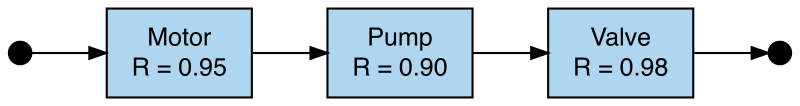
\includegraphics[width=2.67in,height=\textheight,keepaspectratio]{images/rbd-series.png}

}

\caption{Series RBD: Motor → Pump → Valve (all must work)}

\end{figure}%

\begin{Shaded}
\begin{Highlighting}[]
\NormalTok{R\_motor }\OtherTok{\textless{}{-}} \FloatTok{0.95}
\NormalTok{R\_pump  }\OtherTok{\textless{}{-}} \FloatTok{0.90}
\NormalTok{R\_valve }\OtherTok{\textless{}{-}} \FloatTok{0.98}

\NormalTok{R\_series }\OtherTok{\textless{}{-}}\NormalTok{ R\_motor }\SpecialCharTok{*}\NormalTok{ R\_pump }\SpecialCharTok{*}\NormalTok{ R\_valve}
\NormalTok{R\_series  }\CommentTok{\# \textasciitilde{}0.838}
\end{Highlighting}
\end{Shaded}

\begin{verbatim}
[1] 0.8379
\end{verbatim}

The system reliability is approximately 83.8\%, lower than any
individual component.

\begin{tcolorbox}[enhanced jigsaw, arc=.35mm, bottomrule=.15mm, bottomtitle=1mm, breakable, colback=white, colbacktitle=quarto-callout-note-color!10!white, colframe=quarto-callout-note-color-frame, coltitle=black, left=2mm, leftrule=.75mm, opacityback=0, opacitybacktitle=0.6, rightrule=.15mm, title=\textcolor{quarto-callout-note-color}{\faInfo}\hspace{0.5em}{Try It}, titlerule=0mm, toprule=.15mm, toptitle=1mm]

A conveyor belt system has 5 components in series with reliabilities
0.98, 0.96, 0.99, 0.94, and 0.97. Calculate the system reliability.

\begin{Shaded}
\begin{Highlighting}[]
\NormalTok{R\_components }\OtherTok{\textless{}{-}} \FunctionTok{c}\NormalTok{(}\FloatTok{0.98}\NormalTok{, }\FloatTok{0.96}\NormalTok{, }\FloatTok{0.99}\NormalTok{, }\FloatTok{0.94}\NormalTok{, }\FloatTok{0.97}\NormalTok{)}
\CommentTok{\# R\_series \textless{}{-} prod(R\_components)}
\end{Highlighting}
\end{Shaded}

Solution

\begin{Shaded}
\begin{Highlighting}[]
\NormalTok{R\_components }\OtherTok{\textless{}{-}} \FunctionTok{c}\NormalTok{(}\FloatTok{0.98}\NormalTok{, }\FloatTok{0.96}\NormalTok{, }\FloatTok{0.99}\NormalTok{, }\FloatTok{0.94}\NormalTok{, }\FloatTok{0.97}\NormalTok{)}
\NormalTok{R\_series }\OtherTok{\textless{}{-}} \FunctionTok{prod}\NormalTok{(R\_components)}
\NormalTok{R\_series  }\CommentTok{\# \textasciitilde{}0.845}
\end{Highlighting}
\end{Shaded}

\begin{verbatim}
[1] 0.8492432
\end{verbatim}

\end{tcolorbox}

\begin{tcolorbox}[enhanced jigsaw, arc=.35mm, bottomrule=.15mm, bottomtitle=1mm, breakable, colback=white, colbacktitle=quarto-callout-tip-color!10!white, colframe=quarto-callout-tip-color-frame, coltitle=black, left=2mm, leftrule=.75mm, opacityback=0, opacitybacktitle=0.6, rightrule=.15mm, title=\textcolor{quarto-callout-tip-color}{\faLightbulb}\hspace{0.5em}{Review}, titlerule=0mm, toprule=.15mm, toptitle=1mm]

In a series system, which component has the greatest influence on system
reliability?

Answer

The \textbf{least reliable} component. It is the bottleneck; improving
it produces the largest gain in system reliability.

\end{tcolorbox}

\section{Parallel Systems}\label{parallel-systems-1}

In a \textbf{parallel} system, only one component needs to function,
through \textbf{active redundancy} (all components operate
simultaneously). The system fails \emph{only} if all components fail at
the same time. Since component failures are assumed to be independent:

\[P(\text{all fail}) = \prod_{i=1}^{n}(1 - R_i)\]

\[R_{\text{sys}} = 1 - \prod_{i=1}^{n}(1 - R_i)\]

Adding parallel components always increases system reliability.

\subsection{Example: Backup Power
System}\label{example-backup-power-system}

A primary generator (R = 0.90) and a standby generator (R = 0.85);
either alone keeps the system running.

\begin{figure}[H]

{\centering 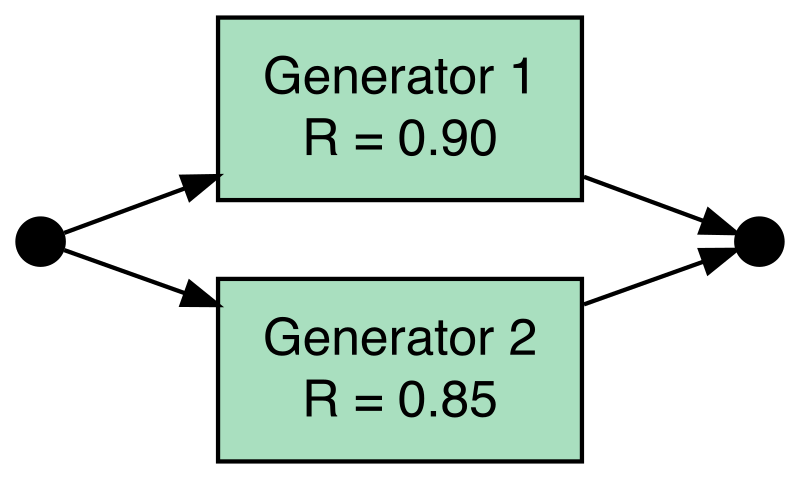
\includegraphics[width=2.67in,height=\textheight,keepaspectratio]{images/rbd-parallel.png}

}

\caption{Parallel RBD: Generator 1 and Generator 2 (either can work)}

\end{figure}%

\begin{Shaded}
\begin{Highlighting}[]
\NormalTok{R\_gen1 }\OtherTok{\textless{}{-}} \FloatTok{0.90}  \CommentTok{\# Generator 1}
\NormalTok{R\_gen2 }\OtherTok{\textless{}{-}} \FloatTok{0.85}  \CommentTok{\# Generator 2}

\NormalTok{R\_parallel }\OtherTok{\textless{}{-}} \DecValTok{1} \SpecialCharTok{{-}}\NormalTok{ (}\DecValTok{1} \SpecialCharTok{{-}}\NormalTok{ R\_gen1) }\SpecialCharTok{*}\NormalTok{ (}\DecValTok{1} \SpecialCharTok{{-}}\NormalTok{ R\_gen2)}
\NormalTok{R\_parallel  }\CommentTok{\# 0.985}
\end{Highlighting}
\end{Shaded}

\begin{verbatim}
[1] 0.985
\end{verbatim}

The parallel system reliability is 98.5\%, much higher than either
generator alone.

The benefit of redundancy grows with each additional component:

\begin{Shaded}
\begin{Highlighting}[]
\NormalTok{n\_vals }\OtherTok{\textless{}{-}} \DecValTok{1}\SpecialCharTok{:}\DecValTok{8}
\NormalTok{Rc     }\OtherTok{\textless{}{-}} \FloatTok{0.90}
\NormalTok{R\_par  }\OtherTok{\textless{}{-}} \DecValTok{1} \SpecialCharTok{{-}}\NormalTok{ (}\DecValTok{1} \SpecialCharTok{{-}}\NormalTok{ Rc)}\SpecialCharTok{\^{}}\NormalTok{n\_vals}

\FunctionTok{plot}\NormalTok{(n\_vals, R\_par, }\AttributeTok{type =} \StringTok{"b"}\NormalTok{, }\AttributeTok{col =} \StringTok{"steelblue"}\NormalTok{, }\AttributeTok{lwd =} \DecValTok{2}\NormalTok{, }\AttributeTok{pch =} \DecValTok{19}\NormalTok{,}
     \AttributeTok{xlab =} \StringTok{"Number of redundant components"}\NormalTok{,}
     \AttributeTok{ylab =} \StringTok{"System Reliability"}\NormalTok{,}
     \AttributeTok{main =} \StringTok{"Parallel System Reliability vs. Redundancy (R\_component = 0.90)"}\NormalTok{,}
     \AttributeTok{ylim =} \FunctionTok{c}\NormalTok{(}\DecValTok{0}\NormalTok{, }\DecValTok{1}\NormalTok{))}
\FunctionTok{abline}\NormalTok{(}\AttributeTok{h =}\NormalTok{ Rc, }\AttributeTok{col =} \StringTok{"gray50"}\NormalTok{, }\AttributeTok{lty =} \DecValTok{2}\NormalTok{)}
\FunctionTok{legend}\NormalTok{(}\StringTok{"bottomright"}\NormalTok{,}
       \AttributeTok{legend =} \FunctionTok{c}\NormalTok{(}\StringTok{"System reliability"}\NormalTok{, }\StringTok{"Single component (0.90)"}\NormalTok{),}
       \AttributeTok{col =} \FunctionTok{c}\NormalTok{(}\StringTok{"steelblue"}\NormalTok{, }\StringTok{"gray50"}\NormalTok{), }\AttributeTok{lty =} \FunctionTok{c}\NormalTok{(}\DecValTok{1}\NormalTok{, }\DecValTok{2}\NormalTok{), }\AttributeTok{pch =} \FunctionTok{c}\NormalTok{(}\DecValTok{19}\NormalTok{, }\ConstantTok{NA}\NormalTok{), }\AttributeTok{lwd =} \DecValTok{2}\NormalTok{)}
\end{Highlighting}
\end{Shaded}

\pandocbounded{
\includegraphics[keepaspectratio]{02-rbd_files/figure-pdf/unnamed-chunk-11-1.pdf}}

\begin{tcolorbox}[enhanced jigsaw, arc=.35mm, bottomrule=.15mm, bottomtitle=1mm, breakable, colback=white, colbacktitle=quarto-callout-note-color!10!white, colframe=quarto-callout-note-color-frame, coltitle=black, left=2mm, leftrule=.75mm, opacityback=0, opacitybacktitle=0.6, rightrule=.15mm, title=\textcolor{quarto-callout-note-color}{\faInfo}\hspace{0.5em}{Try It}, titlerule=0mm, toprule=.15mm, toptitle=1mm]

A critical pump station has 3 pumps in parallel. Each pump has
reliability 0.88. What is the system reliability?

\begin{Shaded}
\begin{Highlighting}[]
\NormalTok{R\_components }\OtherTok{\textless{}{-}} \FunctionTok{c}\NormalTok{(}\FloatTok{0.88}\NormalTok{, }\FloatTok{0.88}\NormalTok{, }\FloatTok{0.88}\NormalTok{)}
\CommentTok{\# R\_parallel \textless{}{-} 1 {-} prod(1 {-} R\_components)}
\end{Highlighting}
\end{Shaded}

Solution

\begin{Shaded}
\begin{Highlighting}[]
\NormalTok{R\_components }\OtherTok{\textless{}{-}} \FunctionTok{c}\NormalTok{(}\FloatTok{0.88}\NormalTok{, }\FloatTok{0.88}\NormalTok{, }\FloatTok{0.88}\NormalTok{)}
\NormalTok{R\_parallel }\OtherTok{\textless{}{-}} \DecValTok{1} \SpecialCharTok{{-}} \FunctionTok{prod}\NormalTok{(}\DecValTok{1} \SpecialCharTok{{-}}\NormalTok{ R\_components)}
\NormalTok{R\_parallel  }\CommentTok{\# \textasciitilde{}0.9983}
\end{Highlighting}
\end{Shaded}

\begin{verbatim}
[1] 0.998272
\end{verbatim}

\end{tcolorbox}

\section{Mixed Systems}\label{mixed-systems}

Most real systems combine series and parallel blocks. To analyze a
\textbf{mixed} system, decompose it into subsystems and apply series and
parallel rules step by step, working from the innermost blocks outward.

\subsection{Example: Safety System}\label{example-safety-system}

\begin{itemize}
\tightlist
\item
  \textbf{Subsystem A}: a sensor (R = 0.95) and a transmitter (R = 0.97)
  in series.
\item
  \textbf{Subsystem B}: two redundant actuators (each R = 0.90) in
  parallel.
\item
  Subsystems A and B in series (both must work).
\end{itemize}

\begin{figure}[H]

{\centering 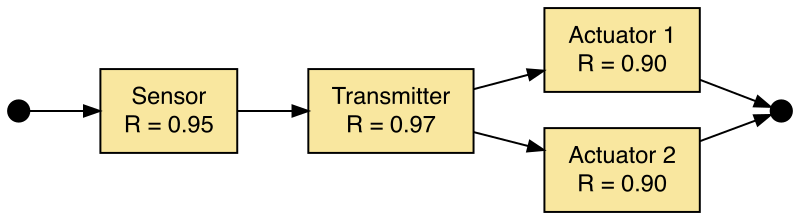
\includegraphics[width=2.67in,height=\textheight,keepaspectratio]{images/rbd-mixed.png}

}

\caption{Mixed RBD: Sensor--Transmitter in series, Actuators 1 \& 2 in
parallel}

\end{figure}%

\begin{Shaded}
\begin{Highlighting}[]
\CommentTok{\# Subsystem A (series)}
\NormalTok{R\_A }\OtherTok{\textless{}{-}} \FloatTok{0.95} \SpecialCharTok{*} \FloatTok{0.97}
\NormalTok{R\_A}
\end{Highlighting}
\end{Shaded}

\begin{verbatim}
[1] 0.9215
\end{verbatim}

\begin{Shaded}
\begin{Highlighting}[]
\CommentTok{\# Subsystem B (parallel)}
\NormalTok{R\_B }\OtherTok{\textless{}{-}} \DecValTok{1} \SpecialCharTok{{-}}\NormalTok{ (}\DecValTok{1} \SpecialCharTok{{-}} \FloatTok{0.90}\NormalTok{) }\SpecialCharTok{*}\NormalTok{ (}\DecValTok{1} \SpecialCharTok{{-}} \FloatTok{0.90}\NormalTok{)}
\NormalTok{R\_B}
\end{Highlighting}
\end{Shaded}

\begin{verbatim}
[1] 0.99
\end{verbatim}

\begin{Shaded}
\begin{Highlighting}[]
\CommentTok{\# Overall system (A and B in series)}
\NormalTok{R\_system }\OtherTok{\textless{}{-}}\NormalTok{ R\_A }\SpecialCharTok{*}\NormalTok{ R\_B}
\NormalTok{R\_system}
\end{Highlighting}
\end{Shaded}

\begin{verbatim}
[1] 0.912285
\end{verbatim}

\begin{tcolorbox}[enhanced jigsaw, arc=.35mm, bottomrule=.15mm, bottomtitle=1mm, breakable, colback=white, colbacktitle=quarto-callout-tip-color!10!white, colframe=quarto-callout-tip-color-frame, coltitle=black, left=2mm, leftrule=.75mm, opacityback=0, opacitybacktitle=0.6, rightrule=.15mm, title=\textcolor{quarto-callout-tip-color}{\faLightbulb}\hspace{0.5em}{Review}, titlerule=0mm, toprule=.15mm, toptitle=1mm]

A system has two subsystems in series. Subsystem 1 has two components in
parallel (each R = 0.85); Subsystem 2 is a single component with R =
0.92. What is the system reliability?

Answer

\(R_{\text{sub1}} = 1 - (1 - 0.85)^2 = 0.9775\).
\(R_{\text{sys}} = 0.9775 \times 0.92 \approx 0.899\).

\end{tcolorbox}

\section{k-out-of-n Systems}\label{k-out-of-n-systems}

A \textbf{k-out-of-n} system succeeds if at least \(k\) of its \(n\)
identical components function:

\begin{itemize}
\tightlist
\item
  \(k = n\): all must work → series.
\item
  \(k = 1\): at least one works → parallel.
\item
  \(1 < k < n\): voting or load-sharing system.
\end{itemize}

The reliability of a k-out-of-n system (identical components, each with
reliability \(p\)) follows the binomial distribution:

\[R_{k/n} = \sum_{i=k}^{n} \binom{n}{i} p^i (1-p)^{n-i} = 1 - \text{pbinom}(k-1,\, n,\, 1-p)\]

The compact R expression counts the probability that \emph{at least}
\(k\) components function: \texttt{pbinom(k-1,\ n,\ 1-p)} gives the
probability that \(k-1\) or fewer components work (i.e., the system
fails), and we subtract that from 1.

\subsection{Example: Flight Control
Computers}\label{example-flight-control-computers}

A 2-out-of-3 voter: at least 2 of 3 computers must agree. Each computer
has R = 0.99.

\begin{figure}[H]

{\centering 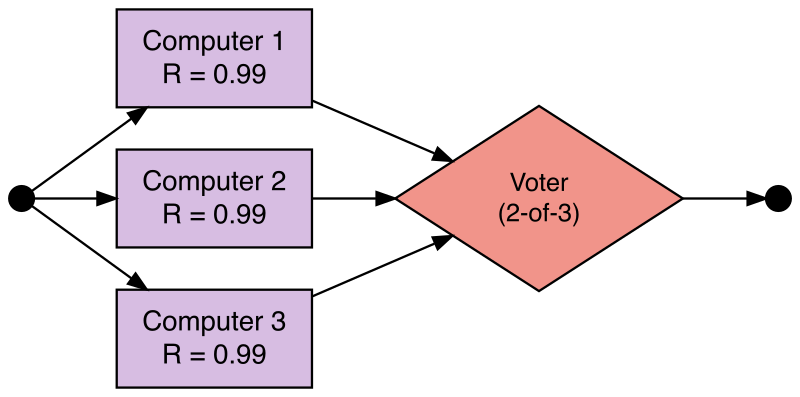
\includegraphics[width=2.67in,height=\textheight,keepaspectratio]{images/rbd-koon.png}

}

\caption{k-out-of-n RBD: 2-of-3 voting system with three computers}

\end{figure}%

\begin{Shaded}
\begin{Highlighting}[]
\NormalTok{n }\OtherTok{\textless{}{-}} \DecValTok{3}      \CommentTok{\# total components}
\NormalTok{k }\OtherTok{\textless{}{-}} \DecValTok{2}      \CommentTok{\# minimum required}
\NormalTok{p }\OtherTok{\textless{}{-}} \FloatTok{0.99}   \CommentTok{\# individual reliability}

\NormalTok{R\_voting }\OtherTok{\textless{}{-}} \DecValTok{1} \SpecialCharTok{{-}} \FunctionTok{pbinom}\NormalTok{(k }\SpecialCharTok{{-}} \DecValTok{1}\NormalTok{, n, }\DecValTok{1} \SpecialCharTok{{-}}\NormalTok{ p)}
\NormalTok{R\_voting  }\CommentTok{\# 0.9997}
\end{Highlighting}
\end{Shaded}

\begin{verbatim}
[1] 0.000298
\end{verbatim}

\begin{tcolorbox}[enhanced jigsaw, arc=.35mm, bottomrule=.15mm, bottomtitle=1mm, breakable, colback=white, colbacktitle=quarto-callout-note-color!10!white, colframe=quarto-callout-note-color-frame, coltitle=black, left=2mm, leftrule=.75mm, opacityback=0, opacitybacktitle=0.6, rightrule=.15mm, title=\textcolor{quarto-callout-note-color}{\faInfo}\hspace{0.5em}{Try It}, titlerule=0mm, toprule=.15mm, toptitle=1mm]

A 3-out-of-5 redundant sensor array. Each sensor has reliability p =
0.95. Calculate the system reliability.

\begin{Shaded}
\begin{Highlighting}[]
\NormalTok{n }\OtherTok{\textless{}{-}} \DecValTok{5}
\NormalTok{k }\OtherTok{\textless{}{-}} \DecValTok{3}
\NormalTok{p }\OtherTok{\textless{}{-}} \FloatTok{0.95}
\CommentTok{\# R\_sys \textless{}{-} 1 {-} pbinom(k {-} 1, n, 1 {-} p)}
\end{Highlighting}
\end{Shaded}

Solution

\begin{Shaded}
\begin{Highlighting}[]
\NormalTok{n }\OtherTok{\textless{}{-}} \DecValTok{5}
\NormalTok{k }\OtherTok{\textless{}{-}} \DecValTok{3}
\NormalTok{p }\OtherTok{\textless{}{-}} \FloatTok{0.95}
\NormalTok{R\_sys }\OtherTok{\textless{}{-}} \DecValTok{1} \SpecialCharTok{{-}} \FunctionTok{pbinom}\NormalTok{(k }\SpecialCharTok{{-}} \DecValTok{1}\NormalTok{, n, }\DecValTok{1} \SpecialCharTok{{-}}\NormalTok{ p)}
\NormalTok{R\_sys  }\CommentTok{\# \textasciitilde{}0.9988}
\end{Highlighting}
\end{Shaded}

\begin{verbatim}
[1] 0.001158125
\end{verbatim}

\end{tcolorbox}

\section{System MTTF}\label{system-mttf}

For a \textbf{series} system of components with constant failure rates,
the system failure rate equals the sum of component failure rates:

\[\lambda_{\text{sys}} = \sum_{i=1}^{n} \lambda_i \qquad \text{MTTF}_{\text{sys}} = \frac{1}{\lambda_{\text{sys}}}\]

For \(n\) identical parallel components each with failure rate
\(\lambda\):

\[\text{MTTF}_{\text{parallel}} = \frac{1}{\lambda}\left(1 + \frac{1}{2} + \frac{1}{3} + \cdots + \frac{1}{n}\right)\]

\subsection{Example: Two Pumps in
Parallel}\label{example-two-pumps-in-parallel}

\begin{Shaded}
\begin{Highlighting}[]
\NormalTok{lambda }\OtherTok{\textless{}{-}} \FloatTok{0.01}  \CommentTok{\# failures per hour}

\NormalTok{MTTF\_single   }\OtherTok{\textless{}{-}} \DecValTok{1} \SpecialCharTok{/}\NormalTok{ lambda}
\NormalTok{MTTF\_parallel }\OtherTok{\textless{}{-}}\NormalTok{ (}\DecValTok{1} \SpecialCharTok{/}\NormalTok{ lambda) }\SpecialCharTok{*}\NormalTok{ (}\DecValTok{1} \SpecialCharTok{+} \DecValTok{1}\SpecialCharTok{/}\DecValTok{2}\NormalTok{)}

\NormalTok{MTTF\_single    }\CommentTok{\# 100 hours}
\end{Highlighting}
\end{Shaded}

\begin{verbatim}
[1] 100
\end{verbatim}

\begin{Shaded}
\begin{Highlighting}[]
\NormalTok{MTTF\_parallel  }\CommentTok{\# 150 hours — 50\% longer with one spare}
\end{Highlighting}
\end{Shaded}

\begin{verbatim}
[1] 150
\end{verbatim}

\begin{tcolorbox}[enhanced jigsaw, arc=.35mm, bottomrule=.15mm, bottomtitle=1mm, breakable, colback=white, colbacktitle=quarto-callout-tip-color!10!white, colframe=quarto-callout-tip-color-frame, coltitle=black, left=2mm, leftrule=.75mm, opacityback=0, opacitybacktitle=0.6, rightrule=.15mm, title=\textcolor{quarto-callout-tip-color}{\faLightbulb}\hspace{0.5em}{Review}, titlerule=0mm, toprule=.15mm, toptitle=1mm]

Three components in series have failure rates 0.02, 0.03, and 0.05
failures/hour. What is the system MTTF?

Answer

\(\lambda_{\text{sys}} = 0.02 + 0.03 + 0.05 = 0.10\), so
\(\text{MTTF} = 1/0.10 = 10\) hours.

\end{tcolorbox}

\section{Common Cause Failure}\label{common-cause-failure}

All the analyses above assume that component failures are
\textbf{statistically independent}: if Component A fails, it tells us
nothing about Component B's probability of failing. In practice, this
assumption can break down.

\textbf{Common Cause Failure (CCF)} occurs when a single event
simultaneously causes multiple components to fail. Typical sources
include:

\begin{itemize}
\tightlist
\item
  A shared environment (vibration, temperature, contamination) that
  degrades all components together
\item
  A common design flaw or manufacturing batch defect
\item
  A maintenance error that affects multiple redundant units at once
\end{itemize}

CCF is especially dangerous because \textbf{redundancy does not protect
against it}: if both pumps in a parallel system can be destroyed by the
same flooding event, adding a third pump does not help.

\subsection{The Beta-Factor Model}\label{the-beta-factor-model}

The simplest CCF model splits each component's total failure rate
\(\lambda\) into two parts:

\[\lambda_{\text{ind}} = (1 - \beta_{\text{CCF}}) \cdot \lambda \qquad \text{(independent failures)}\]
\[\lambda_{\text{CCF}} = \beta_{\text{CCF}} \cdot \lambda \qquad \text{(common-cause failures)}\]

The \textbf{beta-factor} \(\beta_{\text{CCF}}\) is the fraction of
failures attributable to common causes. Typical values range from 0.01
(1\%) for well-separated, dissimilar components to 0.20 (20\%) for
closely coupled identical units.

System reliability for a two-component parallel system with CCF:

\[R_{\text{sys}} = \underbrace{\left[1 - (1 - R_{\text{ind}})^2\right]}_{\text{parallel, independent part}} \times \underbrace{e^{-\lambda_{\text{CCF}} \, t}}_{\text{common-cause part}}\]

\begin{Shaded}
\begin{Highlighting}[]
\NormalTok{lambda }\OtherTok{\textless{}{-}} \FloatTok{0.001}   \CommentTok{\# total component failure rate (per hour)}
\NormalTok{t      }\OtherTok{\textless{}{-}} \DecValTok{1000}    \CommentTok{\# mission time (hours)}

\NormalTok{beta\_vals }\OtherTok{\textless{}{-}} \FunctionTok{c}\NormalTok{(}\DecValTok{0}\NormalTok{, }\FloatTok{0.05}\NormalTok{, }\FloatTok{0.10}\NormalTok{, }\FloatTok{0.20}\NormalTok{)}

\NormalTok{results }\OtherTok{\textless{}{-}} \FunctionTok{sapply}\NormalTok{(beta\_vals, }\ControlFlowTok{function}\NormalTok{(b) \{}
\NormalTok{  R\_ind }\OtherTok{\textless{}{-}} \FunctionTok{exp}\NormalTok{(}\SpecialCharTok{{-}}\NormalTok{(}\DecValTok{1} \SpecialCharTok{{-}}\NormalTok{ b) }\SpecialCharTok{*}\NormalTok{ lambda }\SpecialCharTok{*}\NormalTok{ t)   }\CommentTok{\# independent reliability}
\NormalTok{  R\_ccf }\OtherTok{\textless{}{-}} \FunctionTok{exp}\NormalTok{(}\SpecialCharTok{{-}}\NormalTok{b }\SpecialCharTok{*}\NormalTok{ lambda }\SpecialCharTok{*}\NormalTok{ t)         }\CommentTok{\# common{-}cause reliability}
\NormalTok{  R\_sys }\OtherTok{\textless{}{-}}\NormalTok{ (}\DecValTok{1} \SpecialCharTok{{-}}\NormalTok{ (}\DecValTok{1} \SpecialCharTok{{-}}\NormalTok{ R\_ind)}\SpecialCharTok{\^{}}\DecValTok{2}\NormalTok{) }\SpecialCharTok{*}\NormalTok{ R\_ccf}
  \FunctionTok{round}\NormalTok{(R\_sys, }\DecValTok{4}\NormalTok{)}
\NormalTok{\})}

\FunctionTok{data.frame}\NormalTok{(}\AttributeTok{beta\_CCF =}\NormalTok{ beta\_vals, }\AttributeTok{R\_system =}\NormalTok{ results)}
\end{Highlighting}
\end{Shaded}

\begin{verbatim}
  beta_CCF R_system
1     0.00   0.6004
2     0.05   0.5935
3     0.10   0.5862
4     0.20   0.5705
\end{verbatim}

Even a modest \(\beta_{\text{CCF}} = 0.10\) visibly reduces the system
reliability that redundancy would otherwise provide.

\begin{tcolorbox}[enhanced jigsaw, arc=.35mm, bottomrule=.15mm, bottomtitle=1mm, breakable, colback=white, colbacktitle=quarto-callout-tip-color!10!white, colframe=quarto-callout-tip-color-frame, coltitle=black, left=2mm, leftrule=.75mm, opacityback=0, opacitybacktitle=0.6, rightrule=.15mm, title=\textcolor{quarto-callout-tip-color}{\faLightbulb}\hspace{0.5em}{Review}, titlerule=0mm, toprule=.15mm, toptitle=1mm]

Why doesn't adding more parallel components help when
\(\beta_{\text{CCF}}\) is large?

Answer

When \(\beta_{\text{CCF}}\) is large, a significant fraction of failures
are \textbf{common cause}, simultaneously affecting all components
regardless of how many there are. Adding more identical, coupled
components may even increase the common-cause failure rate if they share
the same environment or design flaw. Effective mitigation requires
\textbf{diversity} (different designs, manufacturers, or locations)
rather than simple redundancy.

\end{tcolorbox}

CCF data and beta-factor values for different equipment types are
tabulated in IEC 61508 (functional safety) and MIL-HDBK-217F (electronic
reliability). For nuclear applications, the NUREG/CR-5497 handbook
provides detailed CCF databases.

\section{Introduction to Fault Tree
Analysis}\label{introduction-to-fault-tree-analysis}

\textbf{Fault Tree Analysis (FTA)} (Vesely et al. 1981) is a top-down
approach that starts with an undesirable event (the \textbf{top event})
and works backward to identify combinations of component failures that
could cause it.

While an RBD asks ``What must work for the system to succeed?'', a fault
tree asks ``What can cause the system to fail?''

\subsection{Gates}\label{gates}

\begin{itemize}
\tightlist
\item
  \textbf{AND gate}: top event occurs only if \emph{all} inputs occur,
  corresponding to \textbf{parallel} RBD components (all must fail).
\item
  \textbf{OR gate}: top event occurs if \emph{any} input occurs,
  corresponding to \textbf{series} RBD components (any failure causes
  system failure).
\end{itemize}

\subsection{RBD---Fault Tree Duality}\label{rbdfault-tree-duality}

{\def\LTcaptype{none} % do not increment counter
\begin{longtable}[]{@{}
  >{\centering\arraybackslash}p{(\linewidth - 2\tabcolsep) * \real{0.5000}}
  >{\centering\arraybackslash}p{(\linewidth - 2\tabcolsep) * \real{0.5000}}@{}}
\toprule\noalign{}
\begin{minipage}[b]{\linewidth}\centering
RBD configuration
\end{minipage} & \begin{minipage}[b]{\linewidth}\centering
Fault tree gate for system failure
\end{minipage} \\
\midrule\noalign{}
\endhead
\bottomrule\noalign{}
\endlastfoot
Series (all must work) & OR gate (any failure causes system failure) \\
Parallel (any can work) & AND gate (all must fail for system failure) \\
\end{longtable}
}

\begin{figure}[H]

{\centering 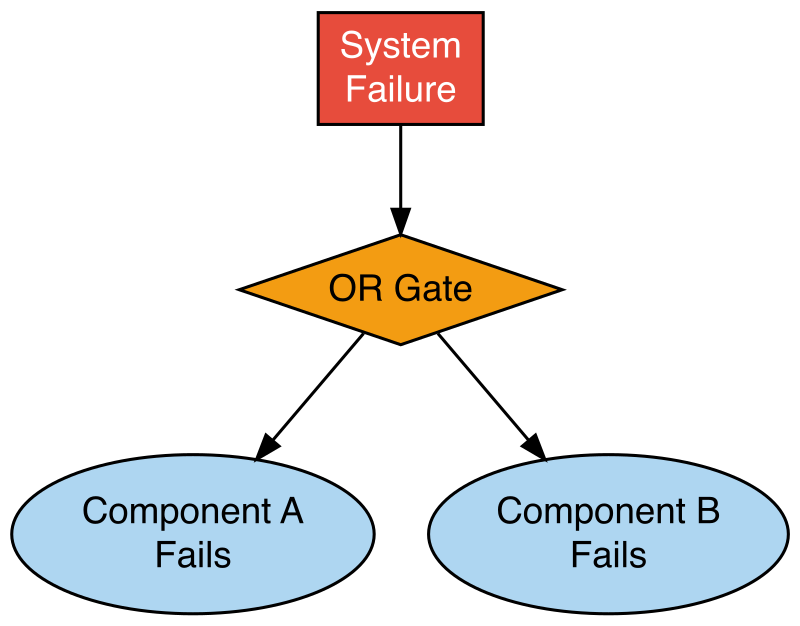
\includegraphics[width=2.67in,height=\textheight,keepaspectratio]{images/rbd-faulttree.png}

}

\caption{Fault Tree: OR gate --- system failure if Component A or B
fails}

\end{figure}%

This OR gate corresponds to a two-component series RBD: any single
failure causes system failure. For complex fault trees, the R package
\texttt{FaultTree} on CRAN provides computational support.

\begin{tcolorbox}[enhanced jigsaw, arc=.35mm, bottomrule=.15mm, bottomtitle=1mm, breakable, colback=white, colbacktitle=quarto-callout-tip-color!10!white, colframe=quarto-callout-tip-color-frame, coltitle=black, left=2mm, leftrule=.75mm, opacityback=0, opacitybacktitle=0.6, rightrule=.15mm, title=\textcolor{quarto-callout-tip-color}{\faLightbulb}\hspace{0.5em}{Review}, titlerule=0mm, toprule=.15mm, toptitle=1mm]

A fault tree has an AND gate combining two component failures. Which RBD
configuration does this correspond to?

Answer

\textbf{Parallel}: an AND gate means the system fails only if both
components fail simultaneously, which is exactly the parallel
(redundant) configuration.

\end{tcolorbox}

\section{Case Study: Industrial Cooling
System}\label{case-study-industrial-cooling-system}

An industrial cooling system has the following architecture:

\begin{enumerate}
\def\labelenumi{\arabic{enumi}.}
\tightlist
\item
  \textbf{Water supply subsystem}: two pumps in parallel (each R =
  0.92), followed by a filter in series (R = 0.99).
\item
  \textbf{Control subsystem}: a primary controller (R = 0.97) and a
  backup controller in parallel (R = 0.95).
\item
  Both subsystems must work (series at system level).
\end{enumerate}

\begin{Shaded}
\begin{Highlighting}[]
\CommentTok{\# Step 1 — Water supply subsystem}
\NormalTok{R\_pump\_parallel }\OtherTok{\textless{}{-}} \DecValTok{1} \SpecialCharTok{{-}}\NormalTok{ (}\DecValTok{1} \SpecialCharTok{{-}} \FloatTok{0.92}\NormalTok{)}\SpecialCharTok{\^{}}\DecValTok{2}
\NormalTok{R\_water }\OtherTok{\textless{}{-}}\NormalTok{ R\_pump\_parallel }\SpecialCharTok{*} \FloatTok{0.99}
\NormalTok{R\_water}
\end{Highlighting}
\end{Shaded}

\begin{verbatim}
[1] 0.983664
\end{verbatim}

\begin{Shaded}
\begin{Highlighting}[]
\CommentTok{\# Step 2 — Control subsystem}
\NormalTok{R\_control }\OtherTok{\textless{}{-}} \DecValTok{1} \SpecialCharTok{{-}}\NormalTok{ (}\DecValTok{1} \SpecialCharTok{{-}} \FloatTok{0.97}\NormalTok{) }\SpecialCharTok{*}\NormalTok{ (}\DecValTok{1} \SpecialCharTok{{-}} \FloatTok{0.95}\NormalTok{)}
\NormalTok{R\_control}
\end{Highlighting}
\end{Shaded}

\begin{verbatim}
[1] 0.9985
\end{verbatim}

\begin{Shaded}
\begin{Highlighting}[]
\CommentTok{\# Step 3 — Overall system (both subsystems in series)}
\NormalTok{R\_system }\OtherTok{\textless{}{-}}\NormalTok{ R\_water }\SpecialCharTok{*}\NormalTok{ R\_control}
\NormalTok{R\_system}
\end{Highlighting}
\end{Shaded}

\begin{verbatim}
[1] 0.9821885
\end{verbatim}

\begin{tcolorbox}[enhanced jigsaw, arc=.35mm, bottomrule=.15mm, bottomtitle=1mm, breakable, colback=white, colbacktitle=quarto-callout-note-color!10!white, colframe=quarto-callout-note-color-frame, coltitle=black, left=2mm, leftrule=.75mm, opacityback=0, opacitybacktitle=0.6, rightrule=.15mm, title=\textcolor{quarto-callout-note-color}{\faInfo}\hspace{0.5em}{Try It}, titlerule=0mm, toprule=.15mm, toptitle=1mm]

Modify the case study: the filter is upgraded to R = 0.999. Recalculate
the system reliability.

\begin{Shaded}
\begin{Highlighting}[]
\NormalTok{R\_pump1  }\OtherTok{\textless{}{-}} \FloatTok{0.92}
\NormalTok{R\_pump2  }\OtherTok{\textless{}{-}} \FloatTok{0.92}
\NormalTok{R\_filter }\OtherTok{\textless{}{-}} \FloatTok{0.999}   \CommentTok{\# upgraded from 0.99}
\NormalTok{R\_ctrl1  }\OtherTok{\textless{}{-}} \FloatTok{0.97}
\NormalTok{R\_ctrl2  }\OtherTok{\textless{}{-}} \FloatTok{0.95}
\end{Highlighting}
\end{Shaded}

Solution

\begin{Shaded}
\begin{Highlighting}[]
\NormalTok{R\_pump1  }\OtherTok{\textless{}{-}} \FloatTok{0.92}
\NormalTok{R\_pump2  }\OtherTok{\textless{}{-}} \FloatTok{0.92}
\NormalTok{R\_filter }\OtherTok{\textless{}{-}} \FloatTok{0.999}
\NormalTok{R\_ctrl1  }\OtherTok{\textless{}{-}} \FloatTok{0.97}
\NormalTok{R\_ctrl2  }\OtherTok{\textless{}{-}} \FloatTok{0.95}

\NormalTok{R\_pump\_parallel }\OtherTok{\textless{}{-}} \DecValTok{1} \SpecialCharTok{{-}}\NormalTok{ (}\DecValTok{1} \SpecialCharTok{{-}}\NormalTok{ R\_pump1) }\SpecialCharTok{*}\NormalTok{ (}\DecValTok{1} \SpecialCharTok{{-}}\NormalTok{ R\_pump2)}
\NormalTok{R\_water   }\OtherTok{\textless{}{-}}\NormalTok{ R\_pump\_parallel }\SpecialCharTok{*}\NormalTok{ R\_filter}
\NormalTok{R\_control }\OtherTok{\textless{}{-}} \DecValTok{1} \SpecialCharTok{{-}}\NormalTok{ (}\DecValTok{1} \SpecialCharTok{{-}}\NormalTok{ R\_ctrl1) }\SpecialCharTok{*}\NormalTok{ (}\DecValTok{1} \SpecialCharTok{{-}}\NormalTok{ R\_ctrl2)}
\NormalTok{R\_system  }\OtherTok{\textless{}{-}}\NormalTok{ R\_water }\SpecialCharTok{*}\NormalTok{ R\_control}
\NormalTok{R\_system  }\CommentTok{\# \textasciitilde{}0.985}
\end{Highlighting}
\end{Shaded}

\begin{verbatim}
[1] 0.9911175
\end{verbatim}

\end{tcolorbox}

\section{Summary}\label{summary-1}

\textbf{Key takeaways:}

\begin{itemize}
\tightlist
\item
  \textbf{Series}: \(R_{\text{sys}} = \prod R_i\), every component must
  work; reliability decreases with more components.
\item
  \textbf{Parallel}: \(R_{\text{sys}} = 1 - \prod(1-R_i)\), redundancy;
  only one component needs to work.
\item
  \textbf{Mixed}: decompose into subsystems, apply formulas step by
  step.
\item
  \textbf{k-out-of-n}: \texttt{1\ -\ pbinom(k-1,\ n,\ 1-p)} for
  voting/load-sharing systems.
\item
  \textbf{Series MTTF}: \(1/\sum\lambda_i\); \textbf{Parallel MTTF}:
  \((1/\lambda)\sum_{i=1}^{n}(1/i)\).
\item
  \textbf{Common Cause Failure}: redundancy requires \emph{diversity} to
  be effective; the \(\beta_{\text{CCF}}\) factor quantifies the
  fraction of failures caused by shared events, and adding more
  identical, coupled components does not protect against CCF.
\item
  \textbf{FTA duality}: series RBD ↔ OR gate; parallel RBD ↔ AND gate.
\end{itemize}

\bookmarksetup{startatroot}

\chapter{Life Data Analysis}\label{sec-lda}

\section{Introduction}\label{introduction-2}

\textbf{Life Data Analysis} is the study of how systems function over
time. Life data tells us how long a system will last, when it will
likely fail, and how often it will need maintenance. In reliability
engineering it is often called \textbf{Weibull analysis} because the
Weibull distribution is the dominant model (Abernethy 2004).

\section{Learning Objectives}\label{learning-objectives-2}

By the end of this chapter, you will be able to:

\begin{itemize}
\tightlist
\item
  Describe the purpose of Weibull analysis in reliability engineering.
\item
  Differentiate between types of data censoring: right-censored and
  interval-censored.
\item
  Differentiate between Weibull models: 2-parameter, 3-parameter, and
  Weibayes.
\item
  Apply Median Rank Regression (MRR) and Maximum Likelihood Estimation
  (MLE).
\item
  Compare Weibull and lognormal fits using goodness-of-fit statistics.
\item
  Determine how many failures are needed for reliable Weibull estimates.
\item
  Interpret results using probability plots and contour plots.
\end{itemize}

\section{Life Distributions}\label{life-distributions}

\subsection{The Weibull Distribution}\label{the-weibull-distribution}

The \textbf{Weibull distribution} is a flexible continuous probability
distribution widely used in life data analysis. Its flexibility comes
from a shape parameter \(\beta\) that allows it to mimic the normal,
exponential, and log-normal distributions.

\subsection{The Reliability (Survival)
Function}\label{the-reliability-survival-function}

The Weibull \textbf{reliability} (survival) function is:

\[R(t) = e^{-(t/\eta)^\beta}\]

where \(R(t)\) is the probability of \emph{surviving beyond} time \(t\),
\(\beta\) is the shape parameter, and \(\eta\) is the scale parameter.
The \textbf{CDF} (cumulative probability of failure by time \(t\)) is
its complement: \(F(t) = 1 - R(t)\).

The shape parameter \(\beta\) has a direct physical interpretation:

{\def\LTcaptype{none} % do not increment counter
\begin{longtable}[]{@{}cll@{}}
\toprule\noalign{}
\(\beta\) & Failure rate & Typical cause \\
\midrule\noalign{}
\endhead
\bottomrule\noalign{}
\endlastfoot
\(< 1\) & Decreasing & Infant mortality \\
\(= 1\) & Constant & Random failures (exponential) \\
\(> 1\) & Increasing & Wear-out (fatigue, corrosion, aging) \\
\end{longtable}
}

\begin{Shaded}
\begin{Highlighting}[]
\NormalTok{t    }\OtherTok{\textless{}{-}} \FunctionTok{seq}\NormalTok{(}\DecValTok{0}\NormalTok{, }\DecValTok{50}\NormalTok{, }\AttributeTok{by =} \FloatTok{0.1}\NormalTok{)}
\NormalTok{etas }\OtherTok{\textless{}{-}} \DecValTok{10}

\CommentTok{\# Plot CDFs for three values of beta}
\FunctionTok{plot}\NormalTok{(t, }\FunctionTok{pweibull}\NormalTok{(t, }\AttributeTok{shape =} \FloatTok{0.5}\NormalTok{, }\AttributeTok{scale =}\NormalTok{ etas), }\AttributeTok{type =} \StringTok{"l"}\NormalTok{, }\AttributeTok{col =} \StringTok{"blue"}\NormalTok{,  }\AttributeTok{lwd =} \DecValTok{2}\NormalTok{,}
     \AttributeTok{xlab =} \StringTok{"Time"}\NormalTok{, }\AttributeTok{ylab =} \StringTok{"Cumulative Probability F(t)"}\NormalTok{,}
     \AttributeTok{main =} \StringTok{"Weibull CDF for Different Shape Parameters (η = 10)"}\NormalTok{,}
     \AttributeTok{ylim =} \FunctionTok{c}\NormalTok{(}\DecValTok{0}\NormalTok{, }\DecValTok{1}\NormalTok{))}
\FunctionTok{lines}\NormalTok{(t, }\FunctionTok{pweibull}\NormalTok{(t, }\AttributeTok{shape =} \FloatTok{1.0}\NormalTok{, }\AttributeTok{scale =}\NormalTok{ etas), }\AttributeTok{col =} \StringTok{"red"}\NormalTok{,       }\AttributeTok{lwd =} \DecValTok{2}\NormalTok{)}
\FunctionTok{lines}\NormalTok{(t, }\FunctionTok{pweibull}\NormalTok{(t, }\AttributeTok{shape =} \FloatTok{3.0}\NormalTok{, }\AttributeTok{scale =}\NormalTok{ etas), }\AttributeTok{col =} \StringTok{"darkgreen"}\NormalTok{, }\AttributeTok{lwd =} \DecValTok{2}\NormalTok{)}
\FunctionTok{legend}\NormalTok{(}\StringTok{"topleft"}\NormalTok{,}
       \AttributeTok{legend =} \FunctionTok{c}\NormalTok{(}\StringTok{"β = 0.5 (decreasing rate)"}\NormalTok{, }\StringTok{"β = 1.0 (constant rate)"}\NormalTok{,}
                  \StringTok{"β = 3.0 (increasing rate)"}\NormalTok{),}
       \AttributeTok{col =} \FunctionTok{c}\NormalTok{(}\StringTok{"blue"}\NormalTok{, }\StringTok{"red"}\NormalTok{, }\StringTok{"darkgreen"}\NormalTok{), }\AttributeTok{lwd =} \DecValTok{2}\NormalTok{)}
\end{Highlighting}
\end{Shaded}

\pandocbounded{
\includegraphics[keepaspectratio]{03-lda_files/figure-pdf/unnamed-chunk-1-1.pdf}}

\textbf{Key property}: at \(t = \eta\),
\(F(\eta) = 1 - e^{-1} \approx 63.2\%\) for any value of \(\beta\). This
is why \(\eta\) is called the \textbf{characteristic life}.

\begin{tcolorbox}[enhanced jigsaw, arc=.35mm, bottomrule=.15mm, bottomtitle=1mm, breakable, colback=white, colbacktitle=quarto-callout-tip-color!10!white, colframe=quarto-callout-tip-color-frame, coltitle=black, left=2mm, leftrule=.75mm, opacityback=0, opacitybacktitle=0.6, rightrule=.15mm, title=\textcolor{quarto-callout-tip-color}{\faLightbulb}\hspace{0.5em}{Review}, titlerule=0mm, toprule=.15mm, toptitle=1mm]

Which value of \(\beta\) indicates an increasing failure rate?

Answer

\(\beta > 1\). A shape parameter greater than 1 indicates a wear-out
failure mode where the failure rate increases over time.

\end{tcolorbox}

\section{WeibullR}\label{weibullr}

The \texttt{WeibullR} package (Silkworth and Symynck 2022; Silkworth
2020) is the primary R tool for Weibull analysis.

\subsection{Getting Started}\label{getting-started}

\begin{Shaded}
\begin{Highlighting}[]
\FunctionTok{install.packages}\NormalTok{(}\StringTok{"WeibullR"}\NormalTok{)}
\end{Highlighting}
\end{Shaded}

\begin{Shaded}
\begin{Highlighting}[]
\FunctionTok{library}\NormalTok{(WeibullR)}
\end{Highlighting}
\end{Shaded}

\subsection{Fitting a Weibull Model}\label{fitting-a-weibull-model}

A factory has 5 machines that failed at times 30, 49, 82, 90, and 96.
Use \texttt{MLEw2p()} to fit a 2-parameter Weibull model using Maximum
Likelihood Estimation and display the probability plot.

\begin{Shaded}
\begin{Highlighting}[]
\NormalTok{failures }\OtherTok{\textless{}{-}} \FunctionTok{c}\NormalTok{(}\DecValTok{30}\NormalTok{, }\DecValTok{49}\NormalTok{, }\DecValTok{82}\NormalTok{, }\DecValTok{90}\NormalTok{, }\DecValTok{96}\NormalTok{)}
\NormalTok{fit }\OtherTok{\textless{}{-}} \FunctionTok{MLEw2p}\NormalTok{(failures, }\AttributeTok{bounds =} \ConstantTok{TRUE}\NormalTok{, }\AttributeTok{show =} \ConstantTok{TRUE}\NormalTok{)}
\end{Highlighting}
\end{Shaded}

\pandocbounded{
\includegraphics[keepaspectratio]{03-lda_files/figure-pdf/unnamed-chunk-4-1.pdf}}

\subsection{Reading the Probability
Plot}\label{reading-the-probability-plot}

The \textbf{Weibull probability plot} shows time on the horizontal axis
(log scale) and cumulative unreliability \(F(t)\) on the vertical axis
(log-log scale). This double-log transformation linearizes Weibull data;
the result is a straight line when the Weibull model fits.

\begin{itemize}
\tightlist
\item
  Read off \(F(t)\) at any time to get the probability of failure by
  that time.
\item
  Reliability at time \(t\) is \(R(t) = 1 - F(t)\).
\item
  \(\beta\) (shape) and \(\eta\) (scale) are shown in the legend.
\end{itemize}

\begin{tcolorbox}[enhanced jigsaw, arc=.35mm, bottomrule=.15mm, bottomtitle=1mm, breakable, colback=white, colbacktitle=quarto-callout-note-color!10!white, colframe=quarto-callout-note-color-frame, coltitle=black, left=2mm, leftrule=.75mm, opacityback=0, opacitybacktitle=0.6, rightrule=.15mm, title=\textcolor{quarto-callout-note-color}{\faInfo}\hspace{0.5em}{Try It}, titlerule=0mm, toprule=.15mm, toptitle=1mm]

A batch of industrial pumps failed at times (hours): 120, 205, 310, 445,
590, 780. Use \texttt{MLEw2p()} to fit a 2-parameter Weibull model.

\begin{Shaded}
\begin{Highlighting}[]
\NormalTok{failures }\OtherTok{\textless{}{-}} \FunctionTok{c}\NormalTok{(}\DecValTok{120}\NormalTok{, }\DecValTok{205}\NormalTok{, }\DecValTok{310}\NormalTok{, }\DecValTok{445}\NormalTok{, }\DecValTok{590}\NormalTok{, }\DecValTok{780}\NormalTok{)}
\CommentTok{\# fit \textless{}{-} MLEw2p(failures, show = TRUE)}
\end{Highlighting}
\end{Shaded}

Solution

\begin{Shaded}
\begin{Highlighting}[]
\NormalTok{failures }\OtherTok{\textless{}{-}} \FunctionTok{c}\NormalTok{(}\DecValTok{120}\NormalTok{, }\DecValTok{205}\NormalTok{, }\DecValTok{310}\NormalTok{, }\DecValTok{445}\NormalTok{, }\DecValTok{590}\NormalTok{, }\DecValTok{780}\NormalTok{)}
\NormalTok{fit }\OtherTok{\textless{}{-}} \FunctionTok{MLEw2p}\NormalTok{(failures, }\AttributeTok{show =} \ConstantTok{TRUE}\NormalTok{)}
\end{Highlighting}
\end{Shaded}

\pandocbounded{
\includegraphics[keepaspectratio]{03-lda_files/figure-pdf/unnamed-chunk-6-1.pdf}}

\end{tcolorbox}

\section{Data Censoring}\label{data-censoring}

In life data analysis, data is often \textbf{censored}: the exact time
to failure is not known for all units.

\subsection{Right-Censored Data
(Suspensions)}\label{right-censored-data-suspensions}

\textbf{Right censoring} occurs when a unit has operated for a period of
time without failing (a \textbf{suspension}). The unit was removed from
service before failing.

\begin{Shaded}
\begin{Highlighting}[]
\NormalTok{failures    }\OtherTok{\textless{}{-}} \FunctionTok{c}\NormalTok{(}\DecValTok{30}\NormalTok{, }\DecValTok{49}\NormalTok{, }\DecValTok{82}\NormalTok{, }\DecValTok{90}\NormalTok{, }\DecValTok{96}\NormalTok{)}
\NormalTok{suspensions }\OtherTok{\textless{}{-}} \FunctionTok{c}\NormalTok{(}\DecValTok{100}\NormalTok{, }\DecValTok{45}\NormalTok{, }\DecValTok{10}\NormalTok{)}
\NormalTok{fit }\OtherTok{\textless{}{-}} \FunctionTok{MLEw2p}\NormalTok{(failures, suspensions, }\AttributeTok{bounds =} \ConstantTok{TRUE}\NormalTok{, }\AttributeTok{show =} \ConstantTok{TRUE}\NormalTok{)}
\end{Highlighting}
\end{Shaded}

\pandocbounded{
\includegraphics[keepaspectratio]{03-lda_files/figure-pdf/unnamed-chunk-7-1.pdf}}

Adding suspensions changes the fit: the model accounts for units that
survived longer, adjusting \(\beta\) and \(\eta\) accordingly.

\begin{tcolorbox}[enhanced jigsaw, arc=.35mm, bottomrule=.15mm, bottomtitle=1mm, breakable, colback=white, colbacktitle=quarto-callout-note-color!10!white, colframe=quarto-callout-note-color-frame, coltitle=black, left=2mm, leftrule=.75mm, opacityback=0, opacitybacktitle=0.6, rightrule=.15mm, title=\textcolor{quarto-callout-note-color}{\faInfo}\hspace{0.5em}{Try It}, titlerule=0mm, toprule=.15mm, toptitle=1mm]

Four compressors failed at 50, 85, 130, and 200 hours. Two additional
units were removed at 250 hours without failing. Fit a Weibull model
with suspensions.

\begin{Shaded}
\begin{Highlighting}[]
\NormalTok{failures    }\OtherTok{\textless{}{-}} \FunctionTok{c}\NormalTok{(}\DecValTok{50}\NormalTok{, }\DecValTok{85}\NormalTok{, }\DecValTok{130}\NormalTok{, }\DecValTok{200}\NormalTok{)}
\NormalTok{suspensions }\OtherTok{\textless{}{-}} \FunctionTok{c}\NormalTok{(}\DecValTok{250}\NormalTok{, }\DecValTok{250}\NormalTok{)}
\CommentTok{\# fit \textless{}{-} MLEw2p(failures, suspensions, show = TRUE)}
\end{Highlighting}
\end{Shaded}

Solution

\begin{Shaded}
\begin{Highlighting}[]
\NormalTok{failures    }\OtherTok{\textless{}{-}} \FunctionTok{c}\NormalTok{(}\DecValTok{50}\NormalTok{, }\DecValTok{85}\NormalTok{, }\DecValTok{130}\NormalTok{, }\DecValTok{200}\NormalTok{)}
\NormalTok{suspensions }\OtherTok{\textless{}{-}} \FunctionTok{c}\NormalTok{(}\DecValTok{250}\NormalTok{, }\DecValTok{250}\NormalTok{)}
\NormalTok{fit }\OtherTok{\textless{}{-}} \FunctionTok{MLEw2p}\NormalTok{(failures, suspensions, }\AttributeTok{show =} \ConstantTok{TRUE}\NormalTok{)}
\end{Highlighting}
\end{Shaded}

\pandocbounded{
\includegraphics[keepaspectratio]{03-lda_files/figure-pdf/unnamed-chunk-9-1.pdf}}

\end{tcolorbox}

\subsection{Interval-Censored Data}\label{interval-censored-data}

\textbf{Interval censoring} occurs when failures are only detected
during periodic inspections; the exact failure time is unknown, but it
is known to have occurred within an interval.

\begin{Shaded}
\begin{Highlighting}[]
\NormalTok{inspection\_data }\OtherTok{\textless{}{-}} \FunctionTok{data.frame}\NormalTok{(}
  \AttributeTok{left  =} \FunctionTok{c}\NormalTok{(}\DecValTok{0}\NormalTok{, }\FloatTok{6.12}\NormalTok{, }\FloatTok{19.92}\NormalTok{, }\FloatTok{29.64}\NormalTok{, }\FloatTok{35.4}\NormalTok{, }\FloatTok{39.72}\NormalTok{, }\FloatTok{45.32}\NormalTok{, }\FloatTok{52.32}\NormalTok{),}
  \AttributeTok{right =} \FunctionTok{c}\NormalTok{(}\FloatTok{6.12}\NormalTok{, }\FloatTok{19.92}\NormalTok{, }\FloatTok{29.64}\NormalTok{, }\FloatTok{35.4}\NormalTok{, }\FloatTok{39.72}\NormalTok{, }\FloatTok{45.32}\NormalTok{, }\FloatTok{52.32}\NormalTok{, }\FloatTok{63.48}\NormalTok{),}
  \AttributeTok{qty   =} \FunctionTok{c}\NormalTok{(}\DecValTok{5}\NormalTok{, }\DecValTok{16}\NormalTok{, }\DecValTok{12}\NormalTok{, }\DecValTok{18}\NormalTok{, }\DecValTok{18}\NormalTok{, }\DecValTok{2}\NormalTok{, }\DecValTok{6}\NormalTok{, }\DecValTok{17}\NormalTok{)}
\NormalTok{)}
\NormalTok{suspensions }\OtherTok{\textless{}{-}} \FunctionTok{data.frame}\NormalTok{(}\AttributeTok{time =} \FloatTok{63.48}\NormalTok{, }\AttributeTok{event =} \DecValTok{0}\NormalTok{, }\AttributeTok{qty =} \DecValTok{73}\NormalTok{)}

\NormalTok{obj1 }\OtherTok{\textless{}{-}} \FunctionTok{wblr}\NormalTok{(suspensions, }\AttributeTok{interval =}\NormalTok{ inspection\_data)}
\NormalTok{obj1 }\OtherTok{\textless{}{-}} \FunctionTok{wblr.fit}\NormalTok{(obj1, }\AttributeTok{method.fit =} \StringTok{"mle"}\NormalTok{, }\AttributeTok{col =} \StringTok{"red"}\NormalTok{)}
\NormalTok{obj1 }\OtherTok{\textless{}{-}} \FunctionTok{wblr.conf}\NormalTok{(obj1, }\AttributeTok{method.conf =} \StringTok{"fm"}\NormalTok{, }\AttributeTok{lty =} \DecValTok{2}\NormalTok{)}
\FunctionTok{plot}\NormalTok{(obj1)}
\end{Highlighting}
\end{Shaded}

\pandocbounded{
\includegraphics[keepaspectratio]{03-lda_files/figure-pdf/unnamed-chunk-10-1.pdf}}

Black horizontal lines represent the inspection intervals; the solid red
line is the model fit; dashed red lines are confidence bounds.

\subsection{Grouped Data}\label{grouped-data}

Life data is often collected in groups. The \texttt{qty} column in the
inspection data above indicates how many units failed in each interval:
5 failed between time 0 and 6.12, 16 between 6.12 and 19.92, and so on.

\begin{tcolorbox}[enhanced jigsaw, arc=.35mm, bottomrule=.15mm, bottomtitle=1mm, breakable, colback=white, colbacktitle=quarto-callout-tip-color!10!white, colframe=quarto-callout-tip-color-frame, coltitle=black, left=2mm, leftrule=.75mm, opacityback=0, opacitybacktitle=0.6, rightrule=.15mm, title=\textcolor{quarto-callout-tip-color}{\faLightbulb}\hspace{0.5em}{Review}, titlerule=0mm, toprule=.15mm, toptitle=1mm]

In the interval-censored example above, how many total failures
occurred?

Answer

\(5 + 16 + 12 + 18 + 18 + 2 + 6 + 17 = 94\) failures. The 73 suspensions
were units that did not fail by the last inspection time (63.48). Total
units in the dataset: \(94 + 73 = 167\).

\end{tcolorbox}

\section{Parameter Estimation
Methods}\label{parameter-estimation-methods}

\subsection{MRR vs MLE}\label{mrr-vs-mle}

\textbf{Median Rank Regression (MRR)} estimates parameters by minimizing
the sum of squared errors between observed and predicted values (least
squares).

\textbf{Maximum Likelihood Estimation (MLE)} finds the parameters that
make the observed data most probable: it maximizes the likelihood
function.

Comparing both methods on the same data:

\begin{Shaded}
\begin{Highlighting}[]
\NormalTok{failures    }\OtherTok{\textless{}{-}} \FunctionTok{c}\NormalTok{(}\DecValTok{30}\NormalTok{, }\DecValTok{49}\NormalTok{, }\DecValTok{82}\NormalTok{, }\DecValTok{90}\NormalTok{, }\DecValTok{96}\NormalTok{)}
\NormalTok{suspensions }\OtherTok{\textless{}{-}} \FunctionTok{c}\NormalTok{(}\DecValTok{100}\NormalTok{, }\DecValTok{45}\NormalTok{, }\DecValTok{10}\NormalTok{)}

\NormalTok{MRRfit }\OtherTok{\textless{}{-}} \FunctionTok{wblr.fit}\NormalTok{(}\FunctionTok{wblr}\NormalTok{(failures, suspensions, }\AttributeTok{col =} \StringTok{"blue"}\NormalTok{), }\AttributeTok{method.fit =} \StringTok{"rr"}\NormalTok{)}
\NormalTok{MLEfit }\OtherTok{\textless{}{-}} \FunctionTok{wblr.fit}\NormalTok{(}\FunctionTok{wblr}\NormalTok{(failures, suspensions, }\AttributeTok{col =} \StringTok{"red"}\NormalTok{),  }\AttributeTok{method.fit =} \StringTok{"mle"}\NormalTok{)}
\FunctionTok{plot.wblr}\NormalTok{(}\FunctionTok{list}\NormalTok{(MRRfit, MLEfit))}
\end{Highlighting}
\end{Shaded}

\pandocbounded{
\includegraphics[keepaspectratio]{03-lda_files/figure-pdf/unnamed-chunk-11-1.pdf}}

Both methods fit the same data. Slight differences in \(\beta\) and
\(\eta\) are visible; the better fit can be determined objectively using
the Anderson-Darling statistic. In practice, \textbf{MLE is preferred
for small samples and censored data} (it uses all the information in the
likelihood); \textbf{MRR is adequate for larger, complete datasets} and
is computationally simpler.

\section{Goodness of Fit}\label{goodness-of-fit}

The \textbf{Anderson-Darling (AD) statistic} measures how closely the
fitted CDF matches the empirical distribution. A \textbf{lower AD} value
indicates a better fit:

{\def\LTcaptype{none} % do not increment counter
\begin{longtable}[]{@{}ll@{}}
\toprule\noalign{}
AD Value & Interpretation \\
\midrule\noalign{}
\endhead
\bottomrule\noalign{}
\endlastfoot
\textless{} 0.3 & Good fit \\
0.3 -- 0.6 & Acceptable fit \\
\textgreater{} 0.6 & Poor fit \\
\end{longtable}
}

WeibullR displays the AD statistic in the plot legend. Use it to compare
fitting methods or distributions.

\begin{tcolorbox}[enhanced jigsaw, arc=.35mm, bottomrule=.15mm, bottomtitle=1mm, breakable, colback=white, colbacktitle=quarto-callout-note-color!10!white, colframe=quarto-callout-note-color-frame, coltitle=black, left=2mm, leftrule=.75mm, opacityback=0, opacitybacktitle=0.6, rightrule=.15mm, title=\textcolor{quarto-callout-note-color}{\faInfo}\hspace{0.5em}{Try It}, titlerule=0mm, toprule=.15mm, toptitle=1mm]

Fit the following failure data with both MRR and MLE, then compare their
AD statistics on a combined probability plot.

\begin{Shaded}
\begin{Highlighting}[]
\NormalTok{failures }\OtherTok{\textless{}{-}} \FunctionTok{c}\NormalTok{(}\DecValTok{15}\NormalTok{, }\DecValTok{28}\NormalTok{, }\DecValTok{44}\NormalTok{, }\DecValTok{61}\NormalTok{, }\DecValTok{83}\NormalTok{, }\DecValTok{110}\NormalTok{, }\DecValTok{145}\NormalTok{)}
\end{Highlighting}
\end{Shaded}

Solution

\begin{Shaded}
\begin{Highlighting}[]
\NormalTok{failures }\OtherTok{\textless{}{-}} \FunctionTok{c}\NormalTok{(}\DecValTok{15}\NormalTok{, }\DecValTok{28}\NormalTok{, }\DecValTok{44}\NormalTok{, }\DecValTok{61}\NormalTok{, }\DecValTok{83}\NormalTok{, }\DecValTok{110}\NormalTok{, }\DecValTok{145}\NormalTok{)}
\NormalTok{obj\_mrr }\OtherTok{\textless{}{-}} \FunctionTok{wblr.fit}\NormalTok{(}\FunctionTok{wblr}\NormalTok{(failures, }\AttributeTok{col =} \StringTok{"blue"}\NormalTok{), }\AttributeTok{method.fit =} \StringTok{"rr"}\NormalTok{)}
\NormalTok{obj\_mle }\OtherTok{\textless{}{-}} \FunctionTok{wblr.fit}\NormalTok{(}\FunctionTok{wblr}\NormalTok{(failures, }\AttributeTok{col =} \StringTok{"red"}\NormalTok{),  }\AttributeTok{method.fit =} \StringTok{"mle"}\NormalTok{)}
\FunctionTok{plot.wblr}\NormalTok{(}\FunctionTok{list}\NormalTok{(obj\_mrr, obj\_mle))}
\end{Highlighting}
\end{Shaded}

\pandocbounded{
\includegraphics[keepaspectratio]{03-lda_files/figure-pdf/unnamed-chunk-13-1.pdf}}

\end{tcolorbox}

\section{Choosing a Distribution}\label{choosing-a-distribution}

The Weibull distribution is the default in reliability engineering, but
it is not always the best fit. The \textbf{lognormal} distribution often
fits failure data driven by fatigue crack growth, corrosion, or
cumulative damage, mechanisms where the logarithm of time-to-failure is
normally distributed.

{\def\LTcaptype{none} % do not increment counter
\begin{longtable}[]{@{}
  >{\raggedright\arraybackslash}p{(\linewidth - 2\tabcolsep) * \real{0.5000}}
  >{\raggedright\arraybackslash}p{(\linewidth - 2\tabcolsep) * \real{0.5000}}@{}}
\toprule\noalign{}
\begin{minipage}[b]{\linewidth}\raggedright
Distribution
\end{minipage} & \begin{minipage}[b]{\linewidth}\raggedright
When it tends to fit best
\end{minipage} \\
\midrule\noalign{}
\endhead
\bottomrule\noalign{}
\endlastfoot
Weibull & Wear-out, mechanical fatigue, early-life failures \\
Lognormal & Corrosion, fatigue crack propagation, electronic
degradation \\
\end{longtable}
}

\texttt{wblr.fit()} supports both via the \texttt{dist} argument. The
goodness-of-fit metric in the plot legend (\(r^2\) for rank regression)
is the tiebreaker: \textbf{higher \(r^2\) indicates a better fit}:

\begin{Shaded}
\begin{Highlighting}[]
\NormalTok{failures    }\OtherTok{\textless{}{-}} \FunctionTok{c}\NormalTok{(}\DecValTok{30}\NormalTok{, }\DecValTok{49}\NormalTok{, }\DecValTok{82}\NormalTok{, }\DecValTok{90}\NormalTok{, }\DecValTok{96}\NormalTok{)}
\NormalTok{suspensions }\OtherTok{\textless{}{-}} \FunctionTok{c}\NormalTok{(}\DecValTok{100}\NormalTok{, }\DecValTok{45}\NormalTok{, }\DecValTok{10}\NormalTok{)}

\NormalTok{obj\_wb }\OtherTok{\textless{}{-}} \FunctionTok{wblr.fit}\NormalTok{(}\FunctionTok{wblr}\NormalTok{(failures, suspensions, }\AttributeTok{col =} \StringTok{"blue"}\NormalTok{),}
                   \AttributeTok{method.fit =} \StringTok{"rr"}\NormalTok{)}
\NormalTok{obj\_ln }\OtherTok{\textless{}{-}} \FunctionTok{wblr.fit}\NormalTok{(}\FunctionTok{wblr}\NormalTok{(failures, suspensions, }\AttributeTok{col =} \StringTok{"red"}\NormalTok{),}
                   \AttributeTok{method.fit =} \StringTok{"rr"}\NormalTok{, }\AttributeTok{dist =} \StringTok{"lognormal"}\NormalTok{)}

\FunctionTok{plot.wblr}\NormalTok{(}\FunctionTok{list}\NormalTok{(obj\_wb, obj\_ln),}
          \AttributeTok{main =} \StringTok{"Weibull vs. Lognormal: Goodness{-}of{-}Fit Comparison"}\NormalTok{)}
\end{Highlighting}
\end{Shaded}

\pandocbounded{
\includegraphics[keepaspectratio]{03-lda_files/figure-pdf/unnamed-chunk-14-1.pdf}}

For this dataset, Weibull achieves \(r^2 \approx 0.953\) vs.~lognormal
at \(r^2 \approx 0.914\); Weibull fits better. The choice should be
driven by the data, not by habit.

\begin{tcolorbox}[enhanced jigsaw, arc=.35mm, bottomrule=.15mm, bottomtitle=1mm, breakable, colback=white, colbacktitle=quarto-callout-note-color!10!white, colframe=quarto-callout-note-color-frame, coltitle=black, left=2mm, leftrule=.75mm, opacityback=0, opacitybacktitle=0.6, rightrule=.15mm, title=\textcolor{quarto-callout-note-color}{\faInfo}\hspace{0.5em}{Try It}, titlerule=0mm, toprule=.15mm, toptitle=1mm]

Fit the 3-parameter Weibull failure dataset below with both Weibull and
lognormal distributions. Which fits better?

\begin{Shaded}
\begin{Highlighting}[]
\NormalTok{failures\_3p }\OtherTok{\textless{}{-}} \FunctionTok{c}\NormalTok{(}\FloatTok{3.47}\NormalTok{, }\FloatTok{3.73}\NormalTok{, }\FloatTok{4.05}\NormalTok{, }\FloatTok{4.63}\NormalTok{, }\FloatTok{4.82}\NormalTok{, }\FloatTok{5.85}\NormalTok{, }\FloatTok{5.89}\NormalTok{, }\FloatTok{5.89}\NormalTok{,}
                 \FloatTok{8.17}\NormalTok{, }\FloatTok{10.03}\NormalTok{, }\FloatTok{10.06}\NormalTok{, }\FloatTok{10.50}\NormalTok{, }\FloatTok{11.11}\NormalTok{, }\FloatTok{11.87}\NormalTok{, }\FloatTok{12.21}\NormalTok{)}
\CommentTok{\# obj\_wb \textless{}{-} wblr.fit(wblr(failures\_3p, col = "blue"), method.fit = "rr")}
\CommentTok{\# obj\_ln \textless{}{-} wblr.fit(wblr(failures\_3p, col = "red"),}
\CommentTok{\#                    method.fit = "rr", dist = "lognormal")}
\CommentTok{\# plot.wblr(list(obj\_wb, obj\_ln))}
\end{Highlighting}
\end{Shaded}

Solution

\begin{Shaded}
\begin{Highlighting}[]
\NormalTok{failures\_3p }\OtherTok{\textless{}{-}} \FunctionTok{c}\NormalTok{(}\FloatTok{3.47}\NormalTok{, }\FloatTok{3.73}\NormalTok{, }\FloatTok{4.05}\NormalTok{, }\FloatTok{4.63}\NormalTok{, }\FloatTok{4.82}\NormalTok{, }\FloatTok{5.85}\NormalTok{, }\FloatTok{5.89}\NormalTok{, }\FloatTok{5.89}\NormalTok{,}
                 \FloatTok{8.17}\NormalTok{, }\FloatTok{10.03}\NormalTok{, }\FloatTok{10.06}\NormalTok{, }\FloatTok{10.50}\NormalTok{, }\FloatTok{11.11}\NormalTok{, }\FloatTok{11.87}\NormalTok{, }\FloatTok{12.21}\NormalTok{)}
\NormalTok{obj\_wb }\OtherTok{\textless{}{-}} \FunctionTok{wblr.fit}\NormalTok{(}\FunctionTok{wblr}\NormalTok{(failures\_3p, }\AttributeTok{col =} \StringTok{"blue"}\NormalTok{), }\AttributeTok{method.fit =} \StringTok{"rr"}\NormalTok{)}
\NormalTok{obj\_ln }\OtherTok{\textless{}{-}} \FunctionTok{wblr.fit}\NormalTok{(}\FunctionTok{wblr}\NormalTok{(failures\_3p, }\AttributeTok{col =} \StringTok{"red"}\NormalTok{),}
                   \AttributeTok{method.fit =} \StringTok{"rr"}\NormalTok{, }\AttributeTok{dist =} \StringTok{"lognormal"}\NormalTok{)}
\FunctionTok{plot.wblr}\NormalTok{(}\FunctionTok{list}\NormalTok{(obj\_wb, obj\_ln),}
          \AttributeTok{main =} \StringTok{"Weibull vs. Lognormal"}\NormalTok{)}
\end{Highlighting}
\end{Shaded}

\pandocbounded{
\includegraphics[keepaspectratio]{03-lda_files/figure-pdf/unnamed-chunk-16-1.pdf}}

Compare the \(r^2\) values in the legend. For this dataset the lognormal
often achieves a slightly higher \(r^2\), suggesting cumulative-damage
behavior, where the logarithm of time-to-failure is approximately
normally distributed.

\end{tcolorbox}

\section{Sample Size Considerations}\label{sample-size-considerations}

Weibull parameter estimates are most reliable when based on at least
10--15 \textbf{observed failures}. With fewer failures, uncertainty
grows substantially: confidence bounds widen, \(r^2\) loses
discriminating power, and estimated \(\beta\) and \(\eta\) can deviate
significantly from the true values.

The following code simulates datasets of different sizes from the same
Weibull (\(\beta = 2\), \(\eta = 100\)) and fits each, showing how
confidence bounds tighten as sample size increases:

\begin{Shaded}
\begin{Highlighting}[]
\FunctionTok{set.seed}\NormalTok{(}\DecValTok{42}\NormalTok{)}
\NormalTok{eta\_true }\OtherTok{\textless{}{-}} \DecValTok{100}\NormalTok{; beta\_true }\OtherTok{\textless{}{-}} \DecValTok{2}

\FunctionTok{par}\NormalTok{(}\AttributeTok{mfrow =} \FunctionTok{c}\NormalTok{(}\DecValTok{1}\NormalTok{, }\DecValTok{3}\NormalTok{))}
\ControlFlowTok{for}\NormalTok{ (n }\ControlFlowTok{in} \FunctionTok{c}\NormalTok{(}\DecValTok{5}\NormalTok{, }\DecValTok{15}\NormalTok{, }\DecValTok{30}\NormalTok{)) \{}
\NormalTok{  f   }\OtherTok{\textless{}{-}} \FunctionTok{sort}\NormalTok{(}\FunctionTok{rweibull}\NormalTok{(n, }\AttributeTok{shape =}\NormalTok{ beta\_true, }\AttributeTok{scale =}\NormalTok{ eta\_true))}
\NormalTok{  obj }\OtherTok{\textless{}{-}} \FunctionTok{wblr.conf}\NormalTok{(}\FunctionTok{wblr.fit}\NormalTok{(}\FunctionTok{wblr}\NormalTok{(f, }\AttributeTok{col =} \StringTok{"blue"}\NormalTok{), }\AttributeTok{method.fit =} \StringTok{"mle"}\NormalTok{),}
                   \AttributeTok{method.conf =} \StringTok{"fm"}\NormalTok{)}
  \FunctionTok{plot}\NormalTok{(obj, }\AttributeTok{main =} \FunctionTok{paste0}\NormalTok{(n, }\StringTok{" failures"}\NormalTok{))}
\NormalTok{\}}
\end{Highlighting}
\end{Shaded}

\pandocbounded{
\includegraphics[keepaspectratio]{03-lda_files/figure-pdf/unnamed-chunk-17-1.pdf}}

\begin{Shaded}
\begin{Highlighting}[]
\FunctionTok{par}\NormalTok{(}\AttributeTok{mfrow =} \FunctionTok{c}\NormalTok{(}\DecValTok{1}\NormalTok{, }\DecValTok{1}\NormalTok{))}
\end{Highlighting}
\end{Shaded}

With only 5 failures the confidence bounds span most of the probability
axis. At 30 failures they are narrow enough for confident
decision-making.

\textbf{Practical guidance:}

{\def\LTcaptype{none} % do not increment counter
\begin{longtable}[]{@{}
  >{\raggedright\arraybackslash}p{(\linewidth - 2\tabcolsep) * \real{0.5000}}
  >{\raggedright\arraybackslash}p{(\linewidth - 2\tabcolsep) * \real{0.5000}}@{}}
\toprule\noalign{}
\begin{minipage}[b]{\linewidth}\raggedright
Failures observed
\end{minipage} & \begin{minipage}[b]{\linewidth}\raggedright
Guidance
\end{minipage} \\
\midrule\noalign{}
\endhead
\bottomrule\noalign{}
\endlastfoot
\(< 5\) & Estimates unreliable; use Weibayes (fix \(\beta\) from prior
knowledge) \\
5--10 & Usable with caution; widen safety margins \\
10--20 & Acceptable for most engineering decisions \\
\(> 20\) & Reliable estimates; confidence bounds are tight \\
\end{longtable}
}

When fewer than 5 failures are available, the Weibayes model (next
section) provides a structured way to incorporate prior knowledge about
\(\beta\).

\section{Other Weibull Models}\label{other-weibull-models}

\subsection{The Weibayes Model}\label{the-weibayes-model}

A \textbf{Weibayes} (one-parameter Weibull) has a fixed \(\beta\) based
on prior knowledge or experience. This is appropriate when failure data
are scarce.

\begin{Shaded}
\begin{Highlighting}[]
\NormalTok{failures    }\OtherTok{\textless{}{-}} \FunctionTok{c}\NormalTok{(}\DecValTok{30}\NormalTok{, }\DecValTok{49}\NormalTok{, }\DecValTok{82}\NormalTok{, }\DecValTok{90}\NormalTok{, }\DecValTok{96}\NormalTok{)}
\NormalTok{suspensions }\OtherTok{\textless{}{-}} \FunctionTok{c}\NormalTok{(}\DecValTok{100}\NormalTok{, }\DecValTok{45}\NormalTok{, }\DecValTok{10}\NormalTok{)}

\NormalTok{obj }\OtherTok{\textless{}{-}} \FunctionTok{wblr.fit}\NormalTok{(}\FunctionTok{wblr}\NormalTok{(failures, suspensions, }\AttributeTok{col =} \StringTok{"blue"}\NormalTok{),}
                \AttributeTok{method.fit =} \StringTok{"weibayes"}\NormalTok{, }\AttributeTok{weibayes.beta =} \DecValTok{2}\NormalTok{)}
\FunctionTok{plot}\NormalTok{(obj)}
\end{Highlighting}
\end{Shaded}

\pandocbounded{
\includegraphics[keepaspectratio]{03-lda_files/figure-pdf/unnamed-chunk-18-1.pdf}}

Confidence bounds are not shown for Weibayes because \(\beta\) is fixed
by assumption.

\subsection{The 3-Parameter Weibull}\label{the-3-parameter-weibull}

The \textbf{3-parameter Weibull} adds a failure-free period \(t_0\), the
time before which no failures can occur:

\[R(t) = e^{-((t - t_0)/\eta)^\beta}\]

This is appropriate for components that must age, wear, or fatigue
before they can fail.

\begin{Shaded}
\begin{Highlighting}[]
\NormalTok{failures\_3p }\OtherTok{\textless{}{-}} \FunctionTok{c}\NormalTok{(}
  \FloatTok{3.46623}\NormalTok{,  }\FloatTok{3.73271}\NormalTok{,  }\FloatTok{4.05300}\NormalTok{,  }\FloatTok{4.62870}\NormalTok{,  }\FloatTok{4.81570}\NormalTok{,}
  \FloatTok{5.84517}\NormalTok{,  }\FloatTok{5.88831}\NormalTok{,  }\FloatTok{5.89297}\NormalTok{,  }\FloatTok{8.16836}\NormalTok{, }\FloatTok{10.02799}\NormalTok{,}
 \FloatTok{10.06062}\NormalTok{, }\FloatTok{10.49785}\NormalTok{, }\FloatTok{11.11493}\NormalTok{, }\FloatTok{11.87369}\NormalTok{, }\FloatTok{12.21122}\NormalTok{,}
 \FloatTok{12.51854}\NormalTok{, }\FloatTok{12.91357}\NormalTok{, }\FloatTok{18.04246}\NormalTok{, }\FloatTok{18.20712}\NormalTok{, }\FloatTok{19.57305}\NormalTok{,}
 \FloatTok{21.20873}\NormalTok{, }\FloatTok{30.03917}\NormalTok{, }\FloatTok{34.88001}\NormalTok{, }\FloatTok{36.87355}\NormalTok{, }\FloatTok{53.91168}
\NormalTok{)}

\NormalTok{fit\_3p }\OtherTok{\textless{}{-}} \FunctionTok{wblr.conf}\NormalTok{(}\FunctionTok{wblr.fit}\NormalTok{(}\FunctionTok{wblr}\NormalTok{(failures\_3p), }\AttributeTok{dist =} \StringTok{"weibull3p"}\NormalTok{), }\AttributeTok{col =} \StringTok{"darkgreen"}\NormalTok{)}
\FunctionTok{plot}\NormalTok{(fit\_3p)}
\end{Highlighting}
\end{Shaded}

\pandocbounded{
\includegraphics[keepaspectratio]{03-lda_files/figure-pdf/unnamed-chunk-19-1.pdf}}

The failure-free period is approximately 3.3 time units, visible as the
curve flattening at low probabilities.

\section{Multi-Plots}\label{multi-plots}

Multi-plots overlay multiple Weibull fits on one chart, making
comparisons easy.

\begin{Shaded}
\begin{Highlighting}[]
\NormalTok{failures    }\OtherTok{\textless{}{-}} \FunctionTok{c}\NormalTok{(}\DecValTok{30}\NormalTok{, }\DecValTok{49}\NormalTok{, }\DecValTok{82}\NormalTok{, }\DecValTok{90}\NormalTok{, }\DecValTok{96}\NormalTok{)}
\NormalTok{suspensions }\OtherTok{\textless{}{-}} \FunctionTok{c}\NormalTok{(}\DecValTok{100}\NormalTok{, }\DecValTok{45}\NormalTok{, }\DecValTok{10}\NormalTok{)}

\NormalTok{obj1 }\OtherTok{\textless{}{-}} \FunctionTok{wblr.fit}\NormalTok{(}\FunctionTok{wblr}\NormalTok{(failures),             }\AttributeTok{col =} \StringTok{"red"}\NormalTok{)}
\NormalTok{obj2 }\OtherTok{\textless{}{-}} \FunctionTok{wblr.fit}\NormalTok{(}\FunctionTok{wblr}\NormalTok{(failures, suspensions), }\AttributeTok{col =} \StringTok{"purple"}\NormalTok{)}

\FunctionTok{plot.wblr}\NormalTok{(}\FunctionTok{list}\NormalTok{(obj1, obj2))}
\end{Highlighting}
\end{Shaded}

\pandocbounded{
\includegraphics[keepaspectratio]{03-lda_files/figure-pdf/unnamed-chunk-20-1.pdf}}

The red model (without suspensions) has a higher beta and lower eta than
the purple model (with suspensions). Adding suspensions shifts the
fitted distribution to account for units that survived longer than the
observed failures.

\section{Competing Failure Modes}\label{competing-failure-modes}

When a component can fail in several distinct ways (corrosion, fatigue,
overload), fitting a single Weibull to the combined data produces a poor
fit because each mode has its own distribution.

The approach: fit a separate Weibull to each failure mode, treating
failures from other modes as suspensions.

\begin{Shaded}
\begin{Highlighting}[]
\FunctionTok{set.seed}\NormalTok{(}\DecValTok{123}\NormalTok{)}
\NormalTok{data }\OtherTok{\textless{}{-}} \FunctionTok{data.frame}\NormalTok{(}
  \AttributeTok{time =} \FunctionTok{c}\NormalTok{(}
    \FunctionTok{rweibull}\NormalTok{(}\DecValTok{5}\NormalTok{,   }\FloatTok{0.5}\NormalTok{, }\DecValTok{20}\NormalTok{),   }\CommentTok{\# Failure Mode A}
    \FunctionTok{rweibull}\NormalTok{(}\DecValTok{10}\NormalTok{,  }\DecValTok{1}\NormalTok{,   }\DecValTok{10}\NormalTok{),   }\CommentTok{\# Failure Mode B}
    \FunctionTok{rweibull}\NormalTok{(}\DecValTok{5}\NormalTok{,   }\DecValTok{2}\NormalTok{,    }\DecValTok{5}\NormalTok{),   }\CommentTok{\# Failure Mode C}
    \FunctionTok{rweibull}\NormalTok{(}\DecValTok{100}\NormalTok{, }\DecValTok{2}\NormalTok{,   }\DecValTok{10}\NormalTok{)    }\CommentTok{\# Suspensions}
\NormalTok{  ),}
  \AttributeTok{event =} \FunctionTok{c}\NormalTok{(}\FunctionTok{rep}\NormalTok{(}\DecValTok{1}\NormalTok{, }\DecValTok{20}\NormalTok{), }\FunctionTok{rep}\NormalTok{(}\DecValTok{0}\NormalTok{, }\DecValTok{100}\NormalTok{)),}
  \AttributeTok{failure\_mode =} \FunctionTok{c}\NormalTok{(}\FunctionTok{rep}\NormalTok{(}\StringTok{"A"}\NormalTok{, }\DecValTok{5}\NormalTok{), }\FunctionTok{rep}\NormalTok{(}\StringTok{"B"}\NormalTok{, }\DecValTok{10}\NormalTok{), }\FunctionTok{rep}\NormalTok{(}\StringTok{"C"}\NormalTok{, }\DecValTok{5}\NormalTok{), }\FunctionTok{rep}\NormalTok{(}\StringTok{""}\NormalTok{, }\DecValTok{100}\NormalTok{))}
\NormalTok{)}

\CommentTok{\# Separate dataset per failure mode (others treated as suspensions)}
\NormalTok{dat1 }\OtherTok{\textless{}{-}}\NormalTok{ dat2 }\OtherTok{\textless{}{-}}\NormalTok{ dat3 }\OtherTok{\textless{}{-}}\NormalTok{ data}
\NormalTok{dat1}\SpecialCharTok{$}\NormalTok{event[dat1}\SpecialCharTok{$}\NormalTok{failure\_mode }\SpecialCharTok{!=} \StringTok{"A"}\NormalTok{] }\OtherTok{\textless{}{-}} \DecValTok{0}
\NormalTok{dat2}\SpecialCharTok{$}\NormalTok{event[dat2}\SpecialCharTok{$}\NormalTok{failure\_mode }\SpecialCharTok{!=} \StringTok{"B"}\NormalTok{] }\OtherTok{\textless{}{-}} \DecValTok{0}
\NormalTok{dat3}\SpecialCharTok{$}\NormalTok{event[dat3}\SpecialCharTok{$}\NormalTok{failure\_mode }\SpecialCharTok{!=} \StringTok{"C"}\NormalTok{] }\OtherTok{\textless{}{-}} \DecValTok{0}

\NormalTok{obj1 }\OtherTok{\textless{}{-}} \FunctionTok{wblr.fit}\NormalTok{(}\FunctionTok{wblr}\NormalTok{(dat1, }\AttributeTok{col =} \StringTok{"blue"}\NormalTok{))}
\NormalTok{obj2 }\OtherTok{\textless{}{-}} \FunctionTok{wblr.fit}\NormalTok{(}\FunctionTok{wblr}\NormalTok{(dat2, }\AttributeTok{col =} \StringTok{"red"}\NormalTok{))}
\NormalTok{obj3 }\OtherTok{\textless{}{-}} \FunctionTok{wblr.fit}\NormalTok{(}\FunctionTok{wblr}\NormalTok{(dat3, }\AttributeTok{col =} \StringTok{"orange"}\NormalTok{))}
\FunctionTok{plot.wblr}\NormalTok{(}\FunctionTok{list}\NormalTok{(obj1, obj2, obj3), }\AttributeTok{is.plot.legend =} \ConstantTok{FALSE}\NormalTok{)}
\end{Highlighting}
\end{Shaded}

\pandocbounded{
\includegraphics[keepaspectratio]{03-lda_files/figure-pdf/unnamed-chunk-21-1.pdf}}

Each failure mode has a distinct \(\beta\): Mode A (\(\beta < 1\),
decreasing rate, infant mortality), Mode B (\(\beta \approx 1\),
random), Mode C (\(\beta > 1\), wear-out).

\section{Contour Plots}\label{contour-plots}

A \textbf{contour plot} shows the joint confidence region for \(\beta\)
and \(\eta\). Overlapping contours indicate that two distributions are
not significantly different at the chosen confidence level.

\begin{Shaded}
\begin{Highlighting}[]
\NormalTok{failures }\OtherTok{\textless{}{-}} \FunctionTok{c}\NormalTok{(}\DecValTok{30}\NormalTok{, }\DecValTok{49}\NormalTok{, }\DecValTok{82}\NormalTok{, }\DecValTok{90}\NormalTok{, }\DecValTok{96}\NormalTok{)}
\NormalTok{obj }\OtherTok{\textless{}{-}} \FunctionTok{wblr.conf}\NormalTok{(}
  \FunctionTok{wblr.fit}\NormalTok{(}\FunctionTok{wblr}\NormalTok{(failures, }\AttributeTok{col =} \StringTok{"blue"}\NormalTok{), }\AttributeTok{method.fit =} \StringTok{"mle"}\NormalTok{),}
  \AttributeTok{method.conf =} \StringTok{"lrb"}
\NormalTok{)}
\FunctionTok{plot\_contour}\NormalTok{(obj, }\AttributeTok{CL =} \FloatTok{0.9}\NormalTok{)}
\end{Highlighting}
\end{Shaded}

\pandocbounded{
\includegraphics[keepaspectratio]{03-lda_files/figure-pdf/unnamed-chunk-22-1.pdf}}

\subsection{Comparing Contour Plots}\label{comparing-contour-plots}

\begin{Shaded}
\begin{Highlighting}[]
\NormalTok{obj1 }\OtherTok{\textless{}{-}} \FunctionTok{wblr.conf}\NormalTok{(}
  \FunctionTok{wblr.fit}\NormalTok{(}\FunctionTok{wblr}\NormalTok{(dat1, }\AttributeTok{col =} \StringTok{"blue"}\NormalTok{),   }\AttributeTok{method.fit =} \StringTok{"mle"}\NormalTok{),}
  \AttributeTok{method.conf =} \StringTok{"lrb"}
\NormalTok{)}
\NormalTok{obj2 }\OtherTok{\textless{}{-}} \FunctionTok{wblr.conf}\NormalTok{(}
  \FunctionTok{wblr.fit}\NormalTok{(}\FunctionTok{wblr}\NormalTok{(dat2, }\AttributeTok{col =} \StringTok{"red"}\NormalTok{),    }\AttributeTok{method.fit =} \StringTok{"mle"}\NormalTok{),}
  \AttributeTok{method.conf =} \StringTok{"lrb"}
\NormalTok{)}
\NormalTok{obj3 }\OtherTok{\textless{}{-}} \FunctionTok{wblr.conf}\NormalTok{(}
  \FunctionTok{wblr.fit}\NormalTok{(}\FunctionTok{wblr}\NormalTok{(dat3, }\AttributeTok{col =} \StringTok{"orange"}\NormalTok{), }\AttributeTok{method.fit =} \StringTok{"mle"}\NormalTok{),}
  \AttributeTok{method.conf =} \StringTok{"lrb"}
\NormalTok{)}
\FunctionTok{plot\_contour}\NormalTok{(}\FunctionTok{list}\NormalTok{(obj1, obj2, obj3), }\AttributeTok{CL =} \FloatTok{0.9}\NormalTok{, }\AttributeTok{xlim =} \FunctionTok{c}\NormalTok{(}\DecValTok{1}\NormalTok{, }\DecValTok{1500}\NormalTok{))}
\end{Highlighting}
\end{Shaded}

\pandocbounded{
\includegraphics[keepaspectratio]{03-lda_files/figure-pdf/unnamed-chunk-23-1.pdf}}

Overlapping contours at 90\% confidence level indicate that the three
failure modes are not statistically distinguishable at this confidence
level.

\section{Summary}\label{summary-2}

\textbf{Key takeaways:}

\begin{itemize}
\tightlist
\item
  The Weibull CDF: \(R(t) = e^{-(t/\eta)^\beta}\).
\item
  \(\beta < 1\): decreasing rate (infant mortality); \(\beta = 1\):
  constant (exponential); \(\beta > 1\): increasing (wear-out).
\item
  At \(t = \eta\): \(F(\eta) = 63.2\%\) for any \(\beta\).
\item
  Suspensions are units that did not fail; always include them in the
  analysis.
\item
  MRR and MLE often give slightly different fits; use the AD statistic
  to choose.
\item
  Weibayes is appropriate for scarce data with prior knowledge of
  \(\beta\).
\item
  3-parameter Weibull handles failure-free periods.
\item
  Multi-plots and contour plots are powerful tools for comparing
  distributions.
\end{itemize}

\bookmarksetup{startatroot}

\chapter{Reliability Growth Analysis}\label{sec-rt}

\section{Introduction}\label{introduction-3}

\textbf{Reliability Growth Analysis (RGA)} monitors and improves
reliability over time by analyzing failure data collected during
testing. It identifies trends in the failure rate, confirming whether
corrective actions are having the intended effect.

\section{Learning Objectives}\label{learning-objectives-3}

By the end of this chapter, you will be able to:

\begin{itemize}
\tightlist
\item
  Define key reliability growth concepts: Crow-AMSAA and Duane models.
\item
  Use \texttt{rdt()} to plan a reliability demonstration test (required
  test time and sample size).
\item
  Fit reliability growth models using R.
\item
  Apply the Duane model to assess reliability growth on a log-log plot.
\item
  Apply the Crow-AMSAA model and interpret its shape parameter
  \(\beta\).
\item
  Use piecewise NHPP models to detect design changes during testing.
\item
  Forecast future failures from a fitted growth model using
  \texttt{predict\_rga()} and visualize the result.
\item
  Interpret reliability growth plots and make decisions from the
  results.
\end{itemize}

\section{Reliability Growth Analysis}\label{reliability-growth-analysis}

The \texttt{ReliaGrowR} package (Govan 2024) provides functions for
reliability growth analysis in R.

\begin{Shaded}
\begin{Highlighting}[]
\FunctionTok{library}\NormalTok{(ReliaGrowR)}
\end{Highlighting}
\end{Shaded}

\section{Test Planning}\label{test-planning}

Before analyzing test data, it helps to answer two design questions:
\emph{How long must we test?} and \emph{How many failures should we
expect?} ReliaGrowR provides tools for both.

\subsection{\texorpdfstring{Reliability Demonstration Tests:
\texttt{rdt()}}{Reliability Demonstration Tests: rdt()}}\label{reliability-demonstration-tests-rdt}

A \textbf{Reliability Demonstration Test (RDT)} is a pass/fail test
designed to demonstrate that a product meets a reliability target at a
specified confidence level. \texttt{rdt()} calculates the required test
time given the sample size (or vice versa).

\begin{Shaded}
\begin{Highlighting}[]
\CommentTok{\# How long must we test 10 units to demonstrate R(1000 hrs) \textgreater{}= 0.90}
\CommentTok{\# at 80\% confidence? Assume Weibull shape beta = 2, zero allowable failures.}
\NormalTok{plan }\OtherTok{\textless{}{-}} \FunctionTok{rdt}\NormalTok{(}
  \AttributeTok{target       =} \FloatTok{0.90}\NormalTok{,   }\CommentTok{\# target reliability}
  \AttributeTok{mission\_time =} \DecValTok{1000}\NormalTok{,   }\CommentTok{\# mission time (hours)}
  \AttributeTok{conf\_level   =} \FloatTok{0.80}\NormalTok{,   }\CommentTok{\# confidence level}
  \AttributeTok{beta         =} \DecValTok{2}\NormalTok{,      }\CommentTok{\# assumed Weibull shape parameter}
  \AttributeTok{n            =} \DecValTok{10}      \CommentTok{\# number of test units}
\NormalTok{)}
\FunctionTok{print}\NormalTok{(plan)}
\end{Highlighting}
\end{Shaded}

\begin{verbatim}
Reliability Demonstration Test (RDT) Plan
-----------------------------------------
Distribution:  Weibull 
Weibull Shape Parameter (Beta):  2 
Allowed Failures (f):  0 
Target Reliability:  0.9 
Mission Time:  1000 
Input Sample Size (n):  10 
Required Test Time (T):  1235.94 
\end{verbatim}

Each unit must be tested for approximately 1,236 hours without failure.
If the test passes, we have demonstrated \(R(1000) \geq 0.90\) with 80\%
confidence.

\begin{tcolorbox}[enhanced jigsaw, arc=.35mm, bottomrule=.15mm, bottomtitle=1mm, breakable, colback=white, colbacktitle=quarto-callout-note-color!10!white, colframe=quarto-callout-note-color-frame, coltitle=black, left=2mm, leftrule=.75mm, opacityback=0, opacitybacktitle=0.6, rightrule=.15mm, title=\textcolor{quarto-callout-note-color}{\faInfo}\hspace{0.5em}{Try It}, titlerule=0mm, toprule=.15mm, toptitle=1mm]

Compare the required test time for sample sizes of 5, 10, and 20 units
(keep all other parameters the same). What is the trade-off?

\begin{Shaded}
\begin{Highlighting}[]
\CommentTok{\# Vary n to see the effect on required test time}
\ControlFlowTok{for}\NormalTok{ (n }\ControlFlowTok{in} \FunctionTok{c}\NormalTok{(}\DecValTok{5}\NormalTok{, }\DecValTok{10}\NormalTok{, }\DecValTok{20}\NormalTok{)) \{}
  \CommentTok{\# plan \textless{}{-} rdt(target = 0.90, mission\_time = 1000, conf\_level = 0.80,}
  \CommentTok{\#             beta = 2, n = n)}
  \CommentTok{\# print(plan)}
\NormalTok{\}}
\end{Highlighting}
\end{Shaded}

Solution

\begin{Shaded}
\begin{Highlighting}[]
\ControlFlowTok{for}\NormalTok{ (n }\ControlFlowTok{in} \FunctionTok{c}\NormalTok{(}\DecValTok{5}\NormalTok{, }\DecValTok{10}\NormalTok{, }\DecValTok{20}\NormalTok{)) \{}
\NormalTok{  plan }\OtherTok{\textless{}{-}} \FunctionTok{rdt}\NormalTok{(}\AttributeTok{target =} \FloatTok{0.90}\NormalTok{, }\AttributeTok{mission\_time =} \DecValTok{1000}\NormalTok{, }\AttributeTok{conf\_level =} \FloatTok{0.80}\NormalTok{,}
              \AttributeTok{beta =} \DecValTok{2}\NormalTok{, }\AttributeTok{n =}\NormalTok{ n)}
  \FunctionTok{print}\NormalTok{(plan)}
\NormalTok{\}}
\end{Highlighting}
\end{Shaded}

\begin{verbatim}
Reliability Demonstration Test (RDT) Plan
-----------------------------------------
Distribution:  Weibull 
Weibull Shape Parameter (Beta):  2 
Allowed Failures (f):  0 
Target Reliability:  0.9 
Mission Time:  1000 
Input Sample Size (n):  5 
Required Test Time (T):  1747.89 
Reliability Demonstration Test (RDT) Plan
-----------------------------------------
Distribution:  Weibull 
Weibull Shape Parameter (Beta):  2 
Allowed Failures (f):  0 
Target Reliability:  0.9 
Mission Time:  1000 
Input Sample Size (n):  10 
Required Test Time (T):  1235.94 
Reliability Demonstration Test (RDT) Plan
-----------------------------------------
Distribution:  Weibull 
Weibull Shape Parameter (Beta):  2 
Allowed Failures (f):  0 
Target Reliability:  0.9 
Mission Time:  1000 
Input Sample Size (n):  20 
Required Test Time (T):  873.94 
\end{verbatim}

More test units means shorter required test time per unit, but total
test effort (n × T) stays roughly constant. Larger fleets reduce
calendar time at the cost of more physical units.

\end{tcolorbox}

\section{The Duane Model}\label{the-duane-model}

The \textbf{Duane Model} (Duane 1964) is one of the earliest and most
widely used models for reliability growth. It is a log-log plot of
cumulative MTBF vs cumulative time, where the MTBF is the total
operating time divided by the number of failures up to that time.

\[\text{CMTBF}(t) = K \cdot t^{\beta - 1}\]

where \(K > 0\) is a scale parameter estimated from the data and
\(\beta\) is the growth slope. The slope of the line on the log-log plot
indicates the rate of reliability growth:

{\def\LTcaptype{none} % do not increment counter
\begin{longtable}[]{@{}cl@{}}
\toprule\noalign{}
Slope (\(\beta\)) & Meaning \\
\midrule\noalign{}
\endhead
\bottomrule\noalign{}
\endlastfoot
\(> 1\) & Reliability improving (failure rate decreasing) \\
\(= 1\) & No change (stable) \\
\(< 1\) & Reliability worsening (failure rate increasing) \\
\end{longtable}
}

Plotting the Duane model for three beta values:

\begin{Shaded}
\begin{Highlighting}[]
\NormalTok{t }\OtherTok{\textless{}{-}} \FunctionTok{seq}\NormalTok{(}\DecValTok{1}\NormalTok{, }\DecValTok{100}\NormalTok{, }\AttributeTok{by =} \FloatTok{0.1}\NormalTok{)}

\CommentTok{\# Three scenarios}
\FunctionTok{plot}\NormalTok{(}\FunctionTok{log}\NormalTok{(t), }\FunctionTok{log}\NormalTok{(}\FloatTok{0.1} \SpecialCharTok{*}\NormalTok{ t}\SpecialCharTok{\^{}}\NormalTok{(}\FloatTok{1.5} \SpecialCharTok{{-}} \DecValTok{1}\NormalTok{)), }\AttributeTok{type =} \StringTok{"l"}\NormalTok{, }\AttributeTok{col =} \StringTok{"blue"}\NormalTok{, }\AttributeTok{lwd =} \DecValTok{2}\NormalTok{,}
     \AttributeTok{xlab =} \StringTok{"log(Cumulative Time)"}\NormalTok{, }\AttributeTok{ylab =} \StringTok{"log(Cumulative MTBF)"}\NormalTok{,}
     \AttributeTok{main =} \StringTok{"Duane Plot: Three Reliability Growth Scenarios"}\NormalTok{,}
     \AttributeTok{ylim =} \FunctionTok{c}\NormalTok{(}\SpecialCharTok{{-}}\DecValTok{4}\NormalTok{, }\DecValTok{1}\NormalTok{))}
\FunctionTok{lines}\NormalTok{(}\FunctionTok{log}\NormalTok{(t), }\FunctionTok{log}\NormalTok{(}\FloatTok{0.1} \SpecialCharTok{*}\NormalTok{ t}\SpecialCharTok{\^{}}\NormalTok{(}\FloatTok{1.0} \SpecialCharTok{{-}} \DecValTok{1}\NormalTok{)), }\AttributeTok{col =} \StringTok{"red"}\NormalTok{,       }\AttributeTok{lwd =} \DecValTok{2}\NormalTok{)}
\FunctionTok{lines}\NormalTok{(}\FunctionTok{log}\NormalTok{(t), }\FunctionTok{log}\NormalTok{(}\FloatTok{0.1} \SpecialCharTok{*}\NormalTok{ t}\SpecialCharTok{\^{}}\NormalTok{(}\FloatTok{0.6} \SpecialCharTok{{-}} \DecValTok{1}\NormalTok{)), }\AttributeTok{col =} \StringTok{"darkgreen"}\NormalTok{, }\AttributeTok{lwd =} \DecValTok{2}\NormalTok{)}
\FunctionTok{legend}\NormalTok{(}\StringTok{"topleft"}\NormalTok{,}
       \AttributeTok{legend =} \FunctionTok{c}\NormalTok{(}\StringTok{"β = 1.5 (improving)"}\NormalTok{, }\StringTok{"β = 1.0 (stable)"}\NormalTok{, }\StringTok{"β = 0.6 (worsening)"}\NormalTok{),}
       \AttributeTok{col =} \FunctionTok{c}\NormalTok{(}\StringTok{"blue"}\NormalTok{, }\StringTok{"red"}\NormalTok{, }\StringTok{"darkgreen"}\NormalTok{), }\AttributeTok{lwd =} \DecValTok{2}\NormalTok{)}
\end{Highlighting}
\end{Shaded}

\pandocbounded{
\includegraphics[keepaspectratio]{04-rt_files/figure-pdf/unnamed-chunk-5-1.pdf}}

\subsection{Fitting with ReliaGrowR}\label{fitting-with-reliagrowr}

\begin{Shaded}
\begin{Highlighting}[]
\NormalTok{times    }\OtherTok{\textless{}{-}} \FunctionTok{c}\NormalTok{(}\DecValTok{100}\NormalTok{, }\DecValTok{200}\NormalTok{, }\DecValTok{300}\NormalTok{, }\DecValTok{400}\NormalTok{, }\DecValTok{500}\NormalTok{)}
\NormalTok{failures }\OtherTok{\textless{}{-}} \FunctionTok{c}\NormalTok{(}\DecValTok{1}\NormalTok{, }\DecValTok{2}\NormalTok{, }\DecValTok{1}\NormalTok{, }\DecValTok{3}\NormalTok{, }\DecValTok{2}\NormalTok{)}

\NormalTok{fit }\OtherTok{\textless{}{-}} \FunctionTok{duane}\NormalTok{(times, failures)}
\FunctionTok{plot}\NormalTok{(fit, }\AttributeTok{main =} \StringTok{"Duane Model Example"}\NormalTok{,}
     \AttributeTok{xlab =} \StringTok{"Cumulative Time"}\NormalTok{, }\AttributeTok{ylab =} \StringTok{"Cumulative MTBF"}\NormalTok{)}
\end{Highlighting}
\end{Shaded}

\pandocbounded{
\includegraphics[keepaspectratio]{04-rt_files/figure-pdf/unnamed-chunk-6-1.pdf}}

\begin{tcolorbox}[enhanced jigsaw, arc=.35mm, bottomrule=.15mm, bottomtitle=1mm, breakable, colback=white, colbacktitle=quarto-callout-note-color!10!white, colframe=quarto-callout-note-color-frame, coltitle=black, left=2mm, leftrule=.75mm, opacityback=0, opacitybacktitle=0.6, rightrule=.15mm, title=\textcolor{quarto-callout-note-color}{\faInfo}\hspace{0.5em}{Try It}, titlerule=0mm, toprule=.15mm, toptitle=1mm]

A new system was tested and the following cumulative failure counts were
recorded. Fit a Duane model and plot the result.

\begin{Shaded}
\begin{Highlighting}[]
\NormalTok{times    }\OtherTok{\textless{}{-}} \FunctionTok{c}\NormalTok{(}\DecValTok{200}\NormalTok{, }\DecValTok{450}\NormalTok{, }\DecValTok{750}\NormalTok{, }\DecValTok{1100}\NormalTok{, }\DecValTok{1500}\NormalTok{, }\DecValTok{2000}\NormalTok{)}
\NormalTok{failures }\OtherTok{\textless{}{-}} \FunctionTok{c}\NormalTok{(}\DecValTok{3}\NormalTok{, }\DecValTok{2}\NormalTok{, }\DecValTok{2}\NormalTok{, }\DecValTok{1}\NormalTok{, }\DecValTok{1}\NormalTok{, }\DecValTok{1}\NormalTok{)}
\CommentTok{\# fit \textless{}{-} duane(times, failures)}
\CommentTok{\# plot(fit)}
\end{Highlighting}
\end{Shaded}

Solution

\begin{Shaded}
\begin{Highlighting}[]
\NormalTok{times    }\OtherTok{\textless{}{-}} \FunctionTok{c}\NormalTok{(}\DecValTok{200}\NormalTok{, }\DecValTok{450}\NormalTok{, }\DecValTok{750}\NormalTok{, }\DecValTok{1100}\NormalTok{, }\DecValTok{1500}\NormalTok{, }\DecValTok{2000}\NormalTok{)}
\NormalTok{failures }\OtherTok{\textless{}{-}} \FunctionTok{c}\NormalTok{(}\DecValTok{3}\NormalTok{, }\DecValTok{2}\NormalTok{, }\DecValTok{2}\NormalTok{, }\DecValTok{1}\NormalTok{, }\DecValTok{1}\NormalTok{, }\DecValTok{1}\NormalTok{)}
\NormalTok{fit }\OtherTok{\textless{}{-}} \FunctionTok{duane}\NormalTok{(times, failures)}
\FunctionTok{plot}\NormalTok{(fit, }\AttributeTok{main =} \StringTok{"Duane Reliability Growth Plot"}\NormalTok{,}
     \AttributeTok{xlab =} \StringTok{"Cumulative Test Time"}\NormalTok{, }\AttributeTok{ylab =} \StringTok{"Cumulative MTBF"}\NormalTok{)}
\end{Highlighting}
\end{Shaded}

\pandocbounded{
\includegraphics[keepaspectratio]{04-rt_files/figure-pdf/unnamed-chunk-8-1.pdf}}

\end{tcolorbox}

\begin{tcolorbox}[enhanced jigsaw, arc=.35mm, bottomrule=.15mm, bottomtitle=1mm, breakable, colback=white, colbacktitle=quarto-callout-tip-color!10!white, colframe=quarto-callout-tip-color-frame, coltitle=black, left=2mm, leftrule=.75mm, opacityback=0, opacitybacktitle=0.6, rightrule=.15mm, title=\textcolor{quarto-callout-tip-color}{\faLightbulb}\hspace{0.5em}{Review}, titlerule=0mm, toprule=.15mm, toptitle=1mm]

What does a Duane plot with a slope greater than 1 indicate?

Answer

The system's reliability is \textbf{improving}: the failure rate is
decreasing over time.

\end{tcolorbox}

\section{The Crow-AMSAA Model}\label{the-crow-amsaa-model}

The \textbf{Crow-AMSAA Model} (Crow 1975) models cumulative failures vs
cumulative time using a Non-Homogeneous Poisson Process (NHPP):

\[N(t) = \lambda_0 \cdot t^{\beta}\]

where \(\lambda_0 > 0\) is the scale parameter and \(\beta\) is the
shape parameter.

The shape parameter \(\beta\) interpretation:

{\def\LTcaptype{none} % do not increment counter
\begin{longtable}[]{@{}cl@{}}
\toprule\noalign{}
\(\beta\) & Meaning \\
\midrule\noalign{}
\endhead
\bottomrule\noalign{}
\endlastfoot
\(> 1\) & Failures increasing (reliability worsening) \\
\(= 1\) & Constant rate (stable) \\
\(< 1\) & Failures decreasing (reliability improving) \\
\end{longtable}
}

\begin{tcolorbox}[enhanced jigsaw, arc=.35mm, bottomrule=.15mm, bottomtitle=1mm, breakable, colback=white, colbacktitle=quarto-callout-warning-color!10!white, colframe=quarto-callout-warning-color-frame, coltitle=black, left=2mm, leftrule=.75mm, opacityback=0, opacitybacktitle=0.6, rightrule=.15mm, title=\textcolor{quarto-callout-warning-color}{\faExclamationTriangle}\hspace{0.5em}{β Interpretation is Reversed Between Models}, titlerule=0mm, toprule=.15mm, toptitle=1mm]

The Crow-AMSAA \(\beta\) means the \textbf{opposite} of the Duane
\(\beta\):

\begin{itemize}
\tightlist
\item
  \textbf{Duane}: \(\beta > 1\) = reliability \emph{improving} (MTBF is
  rising).
\item
  \textbf{Crow-AMSAA}: \(\beta > 1\) = reliability \emph{worsening}
  (cumulative failures are accelerating).
\end{itemize}

This reversal occurs because Duane plots MTBF (higher is better), while
Crow-AMSAA plots cumulative failures (a lower slope means fewer
failures, so \emph{improving}). Always check which model produced your
\(\beta\) before interpreting the result.

\end{tcolorbox}

\begin{Shaded}
\begin{Highlighting}[]
\NormalTok{t }\OtherTok{\textless{}{-}} \FunctionTok{seq}\NormalTok{(}\FloatTok{0.1}\NormalTok{, }\DecValTok{100}\NormalTok{, }\AttributeTok{by =} \FloatTok{0.1}\NormalTok{)}

\CommentTok{\# Three beta scenarios for cumulative failures}
\FunctionTok{plot}\NormalTok{(t, }\FloatTok{0.5} \SpecialCharTok{*}\NormalTok{ t}\SpecialCharTok{\^{}}\FloatTok{0.6}\NormalTok{, }\AttributeTok{type =} \StringTok{"l"}\NormalTok{, }\AttributeTok{col =} \StringTok{"blue"}\NormalTok{, }\AttributeTok{lwd =} \DecValTok{2}\NormalTok{,}
     \AttributeTok{xlab =} \StringTok{"Cumulative Time"}\NormalTok{, }\AttributeTok{ylab =} \StringTok{"Cumulative Failures"}\NormalTok{,}
     \AttributeTok{main =} \StringTok{"Crow{-}AMSAA: Three Reliability Scenarios"}\NormalTok{,}
     \AttributeTok{ylim =} \FunctionTok{c}\NormalTok{(}\DecValTok{0}\NormalTok{, }\DecValTok{20}\NormalTok{))}
\FunctionTok{lines}\NormalTok{(t, }\FloatTok{0.5} \SpecialCharTok{*}\NormalTok{ t}\SpecialCharTok{\^{}}\FloatTok{1.0}\NormalTok{, }\AttributeTok{col =} \StringTok{"red"}\NormalTok{,       }\AttributeTok{lwd =} \DecValTok{2}\NormalTok{)}
\FunctionTok{lines}\NormalTok{(t, }\FloatTok{0.5} \SpecialCharTok{*}\NormalTok{ t}\SpecialCharTok{\^{}}\FloatTok{1.5}\NormalTok{, }\AttributeTok{col =} \StringTok{"darkgreen"}\NormalTok{, }\AttributeTok{lwd =} \DecValTok{2}\NormalTok{)}
\FunctionTok{legend}\NormalTok{(}\StringTok{"topleft"}\NormalTok{,}
       \AttributeTok{legend =} \FunctionTok{c}\NormalTok{(}\StringTok{"β = 0.6 (improving)"}\NormalTok{, }\StringTok{"β = 1.0 (stable)"}\NormalTok{, }\StringTok{"β = 1.5 (worsening)"}\NormalTok{),}
       \AttributeTok{col =} \FunctionTok{c}\NormalTok{(}\StringTok{"blue"}\NormalTok{, }\StringTok{"red"}\NormalTok{, }\StringTok{"darkgreen"}\NormalTok{), }\AttributeTok{lwd =} \DecValTok{2}\NormalTok{)}
\end{Highlighting}
\end{Shaded}

\pandocbounded{
\includegraphics[keepaspectratio]{04-rt_files/figure-pdf/unnamed-chunk-9-1.pdf}}

\subsection{Fitting with ReliaGrowR}\label{fitting-with-reliagrowr-1}

\begin{Shaded}
\begin{Highlighting}[]
\NormalTok{result }\OtherTok{\textless{}{-}} \FunctionTok{rga}\NormalTok{(times, failures)}
\FunctionTok{plot}\NormalTok{(result, }\AttributeTok{main =} \StringTok{"Crow{-}AMSAA Model Example"}\NormalTok{,}
     \AttributeTok{xlab =} \StringTok{"Cumulative Time"}\NormalTok{, }\AttributeTok{ylab =} \StringTok{"Cumulative Failures"}\NormalTok{)}
\end{Highlighting}
\end{Shaded}

\pandocbounded{
\includegraphics[keepaspectratio]{04-rt_files/figure-pdf/unnamed-chunk-10-1.pdf}}

\begin{tcolorbox}[enhanced jigsaw, arc=.35mm, bottomrule=.15mm, bottomtitle=1mm, breakable, colback=white, colbacktitle=quarto-callout-note-color!10!white, colframe=quarto-callout-note-color-frame, coltitle=black, left=2mm, leftrule=.75mm, opacityback=0, opacitybacktitle=0.6, rightrule=.15mm, title=\textcolor{quarto-callout-note-color}{\faInfo}\hspace{0.5em}{Try It}, titlerule=0mm, toprule=.15mm, toptitle=1mm]

A development test recorded these cumulative failure counts. Use
\texttt{rga()} with \texttt{model\_type\ =\ "Crow-AMSAA"} to fit the
model.

\begin{Shaded}
\begin{Highlighting}[]
\NormalTok{times    }\OtherTok{\textless{}{-}} \FunctionTok{c}\NormalTok{(}\DecValTok{50}\NormalTok{, }\DecValTok{120}\NormalTok{, }\DecValTok{220}\NormalTok{, }\DecValTok{360}\NormalTok{, }\DecValTok{530}\NormalTok{, }\DecValTok{740}\NormalTok{, }\DecValTok{1000}\NormalTok{)}
\NormalTok{failures }\OtherTok{\textless{}{-}} \FunctionTok{c}\NormalTok{(}\DecValTok{4}\NormalTok{, }\DecValTok{3}\NormalTok{, }\DecValTok{3}\NormalTok{, }\DecValTok{2}\NormalTok{, }\DecValTok{2}\NormalTok{, }\DecValTok{1}\NormalTok{, }\DecValTok{1}\NormalTok{)}
\CommentTok{\# fit \textless{}{-} rga(times, failures, model\_type = "Crow{-}AMSAA")}
\CommentTok{\# plot(fit)}
\end{Highlighting}
\end{Shaded}

Solution

\begin{Shaded}
\begin{Highlighting}[]
\NormalTok{times    }\OtherTok{\textless{}{-}} \FunctionTok{c}\NormalTok{(}\DecValTok{50}\NormalTok{, }\DecValTok{120}\NormalTok{, }\DecValTok{220}\NormalTok{, }\DecValTok{360}\NormalTok{, }\DecValTok{530}\NormalTok{, }\DecValTok{740}\NormalTok{, }\DecValTok{1000}\NormalTok{)}
\NormalTok{failures }\OtherTok{\textless{}{-}} \FunctionTok{c}\NormalTok{(}\DecValTok{4}\NormalTok{, }\DecValTok{3}\NormalTok{, }\DecValTok{3}\NormalTok{, }\DecValTok{2}\NormalTok{, }\DecValTok{2}\NormalTok{, }\DecValTok{1}\NormalTok{, }\DecValTok{1}\NormalTok{)}
\NormalTok{fit }\OtherTok{\textless{}{-}} \FunctionTok{rga}\NormalTok{(times, failures, }\AttributeTok{model\_type =} \StringTok{"Crow{-}AMSAA"}\NormalTok{)}
\FunctionTok{plot}\NormalTok{(fit, }\AttributeTok{main =} \StringTok{"Crow{-}AMSAA Reliability Growth"}\NormalTok{,}
     \AttributeTok{xlab =} \StringTok{"Cumulative Test Time"}\NormalTok{, }\AttributeTok{ylab =} \StringTok{"Cumulative Failures"}\NormalTok{)}
\end{Highlighting}
\end{Shaded}

\pandocbounded{
\includegraphics[keepaspectratio]{04-rt_files/figure-pdf/unnamed-chunk-12-1.pdf}}

\end{tcolorbox}

\subsection{The Piecewise NHPP Model}\label{the-piecewise-nhpp-model}

The \textbf{Piecewise NHPP} fits a separate Power Law to each segment of
the time axis, separated by breakpoints. This is useful when a design
change occurs during testing.

\[N_i(t) = N(t_{i-1}) + \lambda_i (t - t_{i-1})^{\beta_i}, \quad t_{i-1} < t \leq t_i\]

\begin{Shaded}
\begin{Highlighting}[]
\NormalTok{times    }\OtherTok{\textless{}{-}} \FunctionTok{c}\NormalTok{(}\DecValTok{25}\NormalTok{, }\DecValTok{55}\NormalTok{, }\DecValTok{97}\NormalTok{, }\DecValTok{146}\NormalTok{, }\DecValTok{201}\NormalTok{, }\DecValTok{268}\NormalTok{, }\DecValTok{341}\NormalTok{, }\DecValTok{423}\NormalTok{, }\DecValTok{513}\NormalTok{, }\DecValTok{609}\NormalTok{, }\DecValTok{710}\NormalTok{, }\DecValTok{820}\NormalTok{, }\DecValTok{940}\NormalTok{, }\DecValTok{1072}\NormalTok{, }\DecValTok{1217}\NormalTok{)}
\NormalTok{failures }\OtherTok{\textless{}{-}} \FunctionTok{c}\NormalTok{(}\DecValTok{1}\NormalTok{, }\DecValTok{1}\NormalTok{, }\DecValTok{2}\NormalTok{, }\DecValTok{4}\NormalTok{, }\DecValTok{4}\NormalTok{, }\DecValTok{1}\NormalTok{, }\DecValTok{1}\NormalTok{, }\DecValTok{2}\NormalTok{, }\DecValTok{1}\NormalTok{, }\DecValTok{4}\NormalTok{, }\DecValTok{1}\NormalTok{, }\DecValTok{1}\NormalTok{, }\DecValTok{3}\NormalTok{, }\DecValTok{3}\NormalTok{, }\DecValTok{4}\NormalTok{)}
\NormalTok{breaks   }\OtherTok{\textless{}{-}} \DecValTok{500}

\NormalTok{result }\OtherTok{\textless{}{-}} \FunctionTok{rga}\NormalTok{(times, failures, }\AttributeTok{model\_type =} \StringTok{"Piecewise NHPP"}\NormalTok{, }\AttributeTok{breaks =}\NormalTok{ breaks)}
\FunctionTok{plot}\NormalTok{(result, }\AttributeTok{main =} \StringTok{"Piecewise NHPP Model"}\NormalTok{,}
     \AttributeTok{xlab =} \StringTok{"Cumulative Time"}\NormalTok{, }\AttributeTok{ylab =} \StringTok{"Cumulative Failures"}\NormalTok{)}
\end{Highlighting}
\end{Shaded}

\pandocbounded{
\includegraphics[keepaspectratio]{04-rt_files/figure-pdf/unnamed-chunk-13-1.pdf}}

The two segments have different slopes; the first segment (pre-change)
has a higher slope than the second (post-change), confirming the design
change reduced the failure rate.

\subsection{Change Point Detection}\label{change-point-detection}

Without a known breakpoint, \texttt{rga()} can detect the change point
automatically:

\begin{Shaded}
\begin{Highlighting}[]
\NormalTok{result\_auto }\OtherTok{\textless{}{-}} \FunctionTok{rga}\NormalTok{(times, failures, }\AttributeTok{model\_type =} \StringTok{"Piecewise NHPP"}\NormalTok{)}
\FunctionTok{plot}\NormalTok{(result\_auto, }\AttributeTok{main =} \StringTok{"Piecewise NHPP with Change Point Detection"}\NormalTok{,}
     \AttributeTok{xlab =} \StringTok{"Cumulative Time"}\NormalTok{, }\AttributeTok{ylab =} \StringTok{"Cumulative Failures"}\NormalTok{)}
\end{Highlighting}
\end{Shaded}

\pandocbounded{
\includegraphics[keepaspectratio]{04-rt_files/figure-pdf/unnamed-chunk-14-1.pdf}}

The automatically detected change point is near time 500, consistent
with the known design change.

\section{\texorpdfstring{Forecasting Growth:
\texttt{predict\_rga()}}{Forecasting Growth: predict\_rga()}}\label{forecasting-growth-predict_rga}

Once a growth test is underway, \texttt{predict\_rga()} projects
cumulative failures beyond the current endpoint, useful for deciding
whether to continue testing or whether a reliability target will be met
by a program deadline.

\begin{Shaded}
\begin{Highlighting}[]
\NormalTok{times    }\OtherTok{\textless{}{-}} \FunctionTok{c}\NormalTok{(}\DecValTok{100}\NormalTok{, }\DecValTok{200}\NormalTok{, }\DecValTok{300}\NormalTok{, }\DecValTok{400}\NormalTok{, }\DecValTok{500}\NormalTok{)}
\NormalTok{failures }\OtherTok{\textless{}{-}} \FunctionTok{c}\NormalTok{(}\DecValTok{1}\NormalTok{, }\DecValTok{2}\NormalTok{, }\DecValTok{1}\NormalTok{, }\DecValTok{3}\NormalTok{, }\DecValTok{2}\NormalTok{)}

\NormalTok{fit  }\OtherTok{\textless{}{-}} \FunctionTok{rga}\NormalTok{(times, failures)}
\NormalTok{pred }\OtherTok{\textless{}{-}} \FunctionTok{predict\_rga}\NormalTok{(fit, }\AttributeTok{times =} \FunctionTok{seq}\NormalTok{(}\DecValTok{600}\NormalTok{, }\DecValTok{1000}\NormalTok{, }\AttributeTok{by =} \DecValTok{100}\NormalTok{))}
\FunctionTok{print}\NormalTok{(pred)}
\end{Highlighting}
\end{Shaded}

\begin{verbatim}
Reliability Growth Forecast (Crow-AMSAA) 
----------------------------------------- 
 Time Cum.Failures Lower (95%) Upper (95%)
  600          4.5         3.7         5.3
  700          5.0         4.2         6.1
  800          5.6         4.6         6.8
  900          6.2         5.0         7.6
 1000          6.7         5.4         8.3
\end{verbatim}

\begin{Shaded}
\begin{Highlighting}[]
\FunctionTok{plot}\NormalTok{(pred, }\AttributeTok{main =} \StringTok{"Crow{-}AMSAA Forecast (600–1000 hrs)"}\NormalTok{,}
     \AttributeTok{xlab =} \StringTok{"Cumulative Time"}\NormalTok{, }\AttributeTok{ylab =} \StringTok{"Cumulative Failures"}\NormalTok{)}
\end{Highlighting}
\end{Shaded}

\pandocbounded{
\includegraphics[keepaspectratio]{04-rt_files/figure-pdf/unnamed-chunk-16-1.pdf}}

The confidence band reflects the uncertainty in the Crow-AMSAA parameter
estimates. A narrow band indicates the growth trend is well
characterized; a wide band suggests more test time is needed.

\begin{tcolorbox}[enhanced jigsaw, arc=.35mm, bottomrule=.15mm, bottomtitle=1mm, breakable, colback=white, colbacktitle=quarto-callout-tip-color!10!white, colframe=quarto-callout-tip-color-frame, coltitle=black, left=2mm, leftrule=.75mm, opacityback=0, opacitybacktitle=0.6, rightrule=.15mm, title=\textcolor{quarto-callout-tip-color}{\faLightbulb}\hspace{0.5em}{Review}, titlerule=0mm, toprule=.15mm, toptitle=1mm]

The fitted model gives \(\hat{\beta} < 1\). Is the system still
improving at time 1,000?

Answer

Yes, for the Crow-AMSAA model, \(\beta < 1\) means the cumulative
failure rate is \textbf{decreasing} (the growth curve is concave), so
reliability is still improving at time 1,000. Testing should continue
until \(\beta\) stabilizes near the growth target.

\end{tcolorbox}

\section{Summary}\label{summary-3}

\textbf{Key takeaways:}

\begin{itemize}
\tightlist
\item
  \textbf{Duane model}: log-log of MTBF vs time; positive slope
  (\(\beta > 1\)) = improving.
\item
  \textbf{Crow-AMSAA}: log of cumulative failures vs time; concave
  downward = improving (\(\beta < 1\)).
\item
  \textbf{Piecewise NHPP}: fits multiple segments; use when a known
  change occurs during testing.
\item
  \textbf{Forecasting}: \texttt{predict\_rga()} projects cumulative
  failures with confidence bounds beyond the current test endpoint.
\item
  For accelerated life testing (Arrhenius, Power Law, relationship
  plots), see Chapter~\ref{sec-alt}.
\end{itemize}

\bookmarksetup{startatroot}

\chapter{Accelerated Life Testing}\label{sec-alt}

\section{Introduction}\label{introduction-4}

\textbf{Accelerated Life Testing (ALT)} (Meeker and Escobar 1998; Nelson
1990) subjects products to elevated stress levels: temperature, voltage,
mechanical load, humidity; to induce failures more quickly than would
occur under normal operating conditions. The acceleration relationship
is then used to translate accelerated-test results into normal-use life
predictions.

This approach is essential when products are designed for long service
lives (years or decades), making it impractical to wait for failures at
use conditions. ALT compresses that time by running tests at higher
stress, then mathematically projecting back to the use environment.

\section{Learning Objectives}\label{learning-objectives-4}

By the end of this chapter, you will be able to:

\begin{itemize}
\tightlist
\item
  Explain the purpose of accelerated life testing and the role of the
  Acceleration Factor.
\item
  Apply the Arrhenius model for temperature-accelerated tests.
\item
  Apply the Power Law model for non-thermal stress acceleration.
\item
  Fit ALT models using the \texttt{WeibullR.ALT} package.
\item
  Interpret probability plots and relationship plots from ALT analyses.
\item
  Use parallelization to constrain the shape parameter across stress
  levels.
\end{itemize}

\section{The Acceleration Factor}\label{the-acceleration-factor}

The \textbf{Acceleration Factor (AF)} quantifies how much faster a
product fails under elevated stress compared to use conditions:

\[\text{Life at use conditions} = AF \times \text{Life at stress conditions}\]

The impact of AF on expected test life:

\begin{Shaded}
\begin{Highlighting}[]
\FunctionTok{library}\NormalTok{(WeibullR.ALT)}
\end{Highlighting}
\end{Shaded}

\begin{Shaded}
\begin{Highlighting}[]
\NormalTok{AF\_vals }\OtherTok{\textless{}{-}} \FunctionTok{seq}\NormalTok{(}\DecValTok{1}\NormalTok{, }\DecValTok{10}\NormalTok{, }\AttributeTok{by =} \FloatTok{0.1}\NormalTok{)}
\NormalTok{life\_normal }\OtherTok{\textless{}{-}} \DecValTok{10000}  \CommentTok{\# assumed normal{-}use life}

\FunctionTok{plot}\NormalTok{(AF\_vals, life\_normal }\SpecialCharTok{/}\NormalTok{ AF\_vals, }\AttributeTok{type =} \StringTok{"l"}\NormalTok{, }\AttributeTok{col =} \StringTok{"blue"}\NormalTok{, }\AttributeTok{lwd =} \DecValTok{2}\NormalTok{,}
     \AttributeTok{xlab =} \StringTok{"Acceleration Factor (AF)"}\NormalTok{,}
     \AttributeTok{ylab =} \StringTok{"Expected Life at Stress Conditions"}\NormalTok{,}
     \AttributeTok{main =} \StringTok{"Effect of Acceleration Factor on Test Life"}\NormalTok{)}
\FunctionTok{abline}\NormalTok{(}\AttributeTok{h =}\NormalTok{ life\_normal }\SpecialCharTok{/} \FunctionTok{c}\NormalTok{(}\DecValTok{2}\NormalTok{, }\DecValTok{5}\NormalTok{, }\DecValTok{10}\NormalTok{), }\AttributeTok{col =} \StringTok{"gray70"}\NormalTok{, }\AttributeTok{lty =} \DecValTok{2}\NormalTok{)}
\end{Highlighting}
\end{Shaded}

\pandocbounded{
\includegraphics[keepaspectratio]{05-alt_files/figure-pdf/unnamed-chunk-2-1.pdf}}

An AF of 5 means the product fails five times faster under test stress:
a 10,000-hour life in the field becomes a 2,000-hour test.

\section{The Arrhenius Model}\label{the-arrhenius-model}

The \textbf{Arrhenius Model} describes the relationship between
temperature and reaction rate, which maps directly to material
degradation and failure:

\[AF = \exp\left(\frac{E_a}{k}\left(\frac{1}{T_{\text{use}}} - \frac{1}{T_{\text{stress}}}\right)\right)\]

Where: - \(E_a\) = activation energy in eV (electron volts) - \(k\) =
Boltzmann constant (\(8.617 \times 10^{-5}\) eV/K) - \(T_{\text{use}}\),
\(T_{\text{stress}}\) = temperatures in Kelvin

Higher activation energies mean the failure mechanism is more sensitive
to temperature; a small temperature increase produces a large change in
failure rate.

\begin{tcolorbox}[enhanced jigsaw, arc=.35mm, bottomrule=.15mm, bottomtitle=1mm, breakable, colback=white, colbacktitle=quarto-callout-note-color!10!white, colframe=quarto-callout-note-color-frame, coltitle=black, left=2mm, leftrule=.75mm, opacityback=0, opacitybacktitle=0.6, rightrule=.15mm, title=\textcolor{quarto-callout-note-color}{\faInfo}\hspace{0.5em}{Choosing Activation Energy}, titlerule=0mm, toprule=.15mm, toptitle=1mm]

\(E_a\) is typically drawn from published literature values for the
specific failure mechanism, or estimated from pilot tests at multiple
temperatures. Representative ranges:

{\def\LTcaptype{none} % do not increment counter
\begin{longtable}[]{@{}lc@{}}
\toprule\noalign{}
Failure mechanism & Typical \(E_a\) (eV) \\
\midrule\noalign{}
\endhead
\bottomrule\noalign{}
\endlastfoot
Corrosion / electromigration & 0.5 -- 1.0 \\
Electrical insulation degradation & 0.4 -- 1.5 \\
Semiconductor oxide breakdown & 0.3 -- 0.7 \\
Thermal fatigue (solder) & 0.2 -- 0.5 \\
\end{longtable}
}

If \(E_a\) is unknown, use a sensitivity analysis across a plausible
range before drawing conclusions.

\end{tcolorbox}

\subsection{WeibullR.ALT: Arrhenius-Lognormal
Example}\label{weibullr.alt-arrhenius-lognormal-example}

The \texttt{WeibullR.ALT} package (Silkworth 2022) extends WeibullR with
ALT models. Data: Class B insulation tested at three oven temperatures
(170, 190, 220°C), from Nelson (1990) Table 4.1.

\begin{Shaded}
\begin{Highlighting}[]
\NormalTok{t41    }\OtherTok{\textless{}{-}} \FunctionTok{NelsonData}\NormalTok{(}\StringTok{"table4.1"}\NormalTok{)}
\NormalTok{set170 }\OtherTok{\textless{}{-}} \FunctionTok{alt.data}\NormalTok{(t41}\SpecialCharTok{$}\NormalTok{C170f, }\AttributeTok{s =}\NormalTok{ t41}\SpecialCharTok{$}\NormalTok{C170s, }\AttributeTok{stress =} \DecValTok{170}\NormalTok{)}
\NormalTok{set190 }\OtherTok{\textless{}{-}} \FunctionTok{alt.data}\NormalTok{(t41}\SpecialCharTok{$}\NormalTok{C190f, }\AttributeTok{s =}\NormalTok{ t41}\SpecialCharTok{$}\NormalTok{C190s, }\AttributeTok{stress =} \DecValTok{190}\NormalTok{)}
\NormalTok{set220 }\OtherTok{\textless{}{-}} \FunctionTok{alt.data}\NormalTok{(t41}\SpecialCharTok{$}\NormalTok{C220f, }\AttributeTok{s =}\NormalTok{ t41}\SpecialCharTok{$}\NormalTok{C220s, }\AttributeTok{stress =} \DecValTok{220}\NormalTok{)}

\NormalTok{arrobj }\OtherTok{\textless{}{-}} \FunctionTok{alt.make}\NormalTok{(}\FunctionTok{list}\NormalTok{(set170, set190, set220),}
                   \AttributeTok{dist =} \StringTok{"lognormal"}\NormalTok{, }\AttributeTok{alt.model =} \StringTok{"arrhenius"}\NormalTok{,}
                   \AttributeTok{method.fit =} \StringTok{"mle"}\NormalTok{, }\AttributeTok{view\_dist\_fits =} \ConstantTok{FALSE}\NormalTok{)}
\end{Highlighting}
\end{Shaded}

The fitted curves shift left as temperature increases; higher
temperature leads to shorter life.

Calculating the AF at 220°C vs 170°C with \(E_a = 1.0\) eV:

\begin{Shaded}
\begin{Highlighting}[]
\NormalTok{E\_a      }\OtherTok{\textless{}{-}} \FloatTok{1.0}
\NormalTok{k        }\OtherTok{\textless{}{-}} \FloatTok{8.617e{-}5}
\NormalTok{T\_use    }\OtherTok{\textless{}{-}} \DecValTok{170} \SpecialCharTok{+} \DecValTok{273}  \CommentTok{\# 443 K}
\NormalTok{T\_stress }\OtherTok{\textless{}{-}} \DecValTok{220} \SpecialCharTok{+} \DecValTok{273}  \CommentTok{\# 493 K}

\NormalTok{AF }\OtherTok{\textless{}{-}} \FunctionTok{exp}\NormalTok{(E\_a }\SpecialCharTok{/}\NormalTok{ k }\SpecialCharTok{*}\NormalTok{ (}\DecValTok{1} \SpecialCharTok{/}\NormalTok{ T\_use }\SpecialCharTok{{-}} \DecValTok{1} \SpecialCharTok{/}\NormalTok{ T\_stress))}
\FunctionTok{cat}\NormalTok{(}\StringTok{"Acceleration Factor at 220°C vs 170°C:"}\NormalTok{, }\FunctionTok{round}\NormalTok{(AF, }\DecValTok{1}\NormalTok{), }\StringTok{"}\SpecialCharTok{\textbackslash{}n}\StringTok{"}\NormalTok{)}
\end{Highlighting}
\end{Shaded}

\begin{verbatim}
Acceleration Factor at 220<U+00B0>C vs 170<U+00B0>C: 14.3 
\end{verbatim}

As printed above, the insulation degrades approximately 14 times faster
at 220°C than at 170°C, a substantial acceleration that compresses a
multi-year test into a much shorter duration.

\begin{tcolorbox}[enhanced jigsaw, arc=.35mm, bottomrule=.15mm, bottomtitle=1mm, breakable, colback=white, colbacktitle=quarto-callout-note-color!10!white, colframe=quarto-callout-note-color-frame, coltitle=black, left=2mm, leftrule=.75mm, opacityback=0, opacitybacktitle=0.6, rightrule=.15mm, title=\textcolor{quarto-callout-note-color}{\faInfo}\hspace{0.5em}{Try It}, titlerule=0mm, toprule=.15mm, toptitle=1mm]

A component is tested at 85°C to accelerate failures. The use
temperature is 25°C. The activation energy is 0.65 eV. Compute the AF.

\begin{Shaded}
\begin{Highlighting}[]
\NormalTok{E\_a      }\OtherTok{\textless{}{-}} \FloatTok{0.65}
\NormalTok{k        }\OtherTok{\textless{}{-}} \FloatTok{8.617e{-}5}
\NormalTok{T\_use    }\OtherTok{\textless{}{-}} \DecValTok{25} \SpecialCharTok{+} \FloatTok{273.15}
\NormalTok{T\_stress }\OtherTok{\textless{}{-}} \DecValTok{85} \SpecialCharTok{+} \FloatTok{273.15}
\CommentTok{\# AF = exp((E\_a / k) * (1/T\_use {-} 1/T\_stress))}
\end{Highlighting}
\end{Shaded}

Solution

\begin{Shaded}
\begin{Highlighting}[]
\NormalTok{E\_a      }\OtherTok{\textless{}{-}} \FloatTok{0.65}
\NormalTok{k        }\OtherTok{\textless{}{-}} \FloatTok{8.617e{-}5}
\NormalTok{T\_use    }\OtherTok{\textless{}{-}} \DecValTok{25} \SpecialCharTok{+} \FloatTok{273.15}
\NormalTok{T\_stress }\OtherTok{\textless{}{-}} \DecValTok{85} \SpecialCharTok{+} \FloatTok{273.15}
\NormalTok{AF }\OtherTok{\textless{}{-}} \FunctionTok{exp}\NormalTok{((E\_a }\SpecialCharTok{/}\NormalTok{ k) }\SpecialCharTok{*}\NormalTok{ (}\DecValTok{1} \SpecialCharTok{/}\NormalTok{ T\_use }\SpecialCharTok{{-}} \DecValTok{1} \SpecialCharTok{/}\NormalTok{ T\_stress))}
\FunctionTok{cat}\NormalTok{(}\StringTok{"Acceleration Factor:"}\NormalTok{, }\FunctionTok{round}\NormalTok{(AF, }\DecValTok{1}\NormalTok{), }\StringTok{"}\SpecialCharTok{\textbackslash{}n}\StringTok{"}\NormalTok{)}
\end{Highlighting}
\end{Shaded}

\begin{verbatim}
Acceleration Factor: 69.3 
\end{verbatim}

\end{tcolorbox}

\section{The Power Law Model}\label{the-power-law-model}

The \textbf{Power Law Model} describes how a product's life is affected
by non-thermal stresses (voltage, mechanical load, pressure):

\[AF = \left(\frac{S_{\text{stress}}}{S_{\text{use}}}\right)^{n}\]

Where \(n\) is the \textbf{stress exponent}, the sensitivity of the
failure mechanism to the applied stress. Typical values range from 1--3
for low-sensitivity mechanisms to 4--8 for voltage-driven dielectric
breakdown. \(n\) is estimated from the ALT data by fitting the model at
multiple stress levels.

\subsection{WeibullR.ALT: Power Law
Example}\label{weibullr.alt-power-law-example}

Data: electrical insulating fluids tested at 7 voltage levels (26--38
kV).

\begin{Shaded}
\begin{Highlighting}[]
\NormalTok{data\_nelson }\OtherTok{\textless{}{-}} \FunctionTok{NelsonData}\NormalTok{(}\StringTok{"table3.1"}\NormalTok{)}

\NormalTok{data26 }\OtherTok{\textless{}{-}} \FunctionTok{alt.data}\NormalTok{(data\_nelson}\SpecialCharTok{$}\NormalTok{kV26, }\AttributeTok{stress =} \DecValTok{26}\NormalTok{)}
\NormalTok{data28 }\OtherTok{\textless{}{-}} \FunctionTok{alt.data}\NormalTok{(data\_nelson}\SpecialCharTok{$}\NormalTok{kV28, }\AttributeTok{stress =} \DecValTok{28}\NormalTok{)}
\NormalTok{data30 }\OtherTok{\textless{}{-}} \FunctionTok{alt.data}\NormalTok{(data\_nelson}\SpecialCharTok{$}\NormalTok{kV30, }\AttributeTok{stress =} \DecValTok{30}\NormalTok{)}
\NormalTok{data32 }\OtherTok{\textless{}{-}} \FunctionTok{alt.data}\NormalTok{(data\_nelson}\SpecialCharTok{$}\NormalTok{kV32, }\AttributeTok{stress =} \DecValTok{32}\NormalTok{)}
\NormalTok{data34 }\OtherTok{\textless{}{-}} \FunctionTok{alt.data}\NormalTok{(data\_nelson}\SpecialCharTok{$}\NormalTok{kV34, }\AttributeTok{stress =} \DecValTok{34}\NormalTok{)}
\NormalTok{data36 }\OtherTok{\textless{}{-}} \FunctionTok{alt.data}\NormalTok{(data\_nelson}\SpecialCharTok{$}\NormalTok{kV36, }\AttributeTok{stress =} \DecValTok{36}\NormalTok{)}
\NormalTok{data38 }\OtherTok{\textless{}{-}} \FunctionTok{alt.data}\NormalTok{(data\_nelson}\SpecialCharTok{$}\NormalTok{kV38, }\AttributeTok{stress =} \DecValTok{38}\NormalTok{)}

\NormalTok{pwrobj }\OtherTok{\textless{}{-}} \FunctionTok{alt.make}\NormalTok{(}\FunctionTok{list}\NormalTok{(data26, data28, data30, data32, data34, data36, data38),}
                   \AttributeTok{dist =} \StringTok{"weibull"}\NormalTok{, }\AttributeTok{alt.model =} \StringTok{"power"}\NormalTok{)}
\end{Highlighting}
\end{Shaded}

\pandocbounded{
\includegraphics[keepaspectratio]{05-alt_files/figure-pdf/unnamed-chunk-7-1.pdf}}

Curves shift left as voltage increases; higher voltage stress leads to
shorter life.

\section{Multiple Stress Factors}\label{multiple-stress-factors}

The \textbf{Eyring Model} extends the Arrhenius approach to account for
multiple stress factors (temperature, voltage, humidity):

\[\text{Life}(S) = A \cdot \exp\left(\frac{B}{S} + C \cdot S\right)\]

The formula above assumes a single primary stress \(S\). For truly
multiple independent stresses (e.g., temperature \emph{and} humidity
\emph{and} voltage), additional terms are added to the exponent. The
\texttt{WeibullR.ALT} package supports the Eyring model via
\texttt{alt.make(...,\ alt.model\ =\ "eyring")}. See the package
documentation for examples.

\section{Parallelization}\label{parallelization}

\textbf{Parallelization} constrains the shape parameter (slope) to be
equal across all stress levels, simplifying the analysis:

\begin{Shaded}
\begin{Highlighting}[]
\NormalTok{prlobj }\OtherTok{\textless{}{-}} \FunctionTok{alt.parallel}\NormalTok{(arrobj)}
\end{Highlighting}
\end{Shaded}

\pandocbounded{
\includegraphics[keepaspectratio]{05-alt_files/figure-pdf/unnamed-chunk-8-1.pdf}}

\begin{Shaded}
\begin{Highlighting}[]
\NormalTok{expobj }\OtherTok{\textless{}{-}} \FunctionTok{alt.parallel}\NormalTok{(pwrobj)}
\end{Highlighting}
\end{Shaded}

\pandocbounded{
\includegraphics[keepaspectratio]{05-alt_files/figure-pdf/unnamed-chunk-8-2.pdf}}

With parallel slopes, the relationship between stress and life can be
characterized by a single line (the relationship plot).

\section{Relationship Plots}\label{relationship-plots}

The \textbf{relationship plot} shows how life changes as stress
increases (log-linear, stress on x-axis, log-life on y-axis). The slope
characterizes the sensitivity of life to stress:

\begin{itemize}
\tightlist
\item
  \textbf{Negative slope}: higher stress → shorter life (typical).
\item
  \textbf{Flat slope}: stress has little effect.
\item
  \textbf{Positive slope}: higher stress → longer life (rare).
\end{itemize}

\begin{Shaded}
\begin{Highlighting}[]
\NormalTok{lnrobj }\OtherTok{\textless{}{-}} \FunctionTok{alt.fit}\NormalTok{(prlobj)}
\FunctionTok{plot}\NormalTok{(lnrobj, }\AttributeTok{suppress.dev.new =} \ConstantTok{TRUE}\NormalTok{)}
\end{Highlighting}
\end{Shaded}

\pandocbounded{
\includegraphics[keepaspectratio]{05-alt_files/figure-pdf/unnamed-chunk-9-1.pdf}}

Each line corresponds to a different probability of failure (e.g., P10 =
10\% failure probability, P63.2 = 63.2\% failure probability =
characteristic life).

\begin{Shaded}
\begin{Highlighting}[]
\NormalTok{lnrobj2 }\OtherTok{\textless{}{-}} \FunctionTok{alt.fit}\NormalTok{(expobj)}
\FunctionTok{plot}\NormalTok{(lnrobj2, }\AttributeTok{suppress.dev.new =} \ConstantTok{TRUE}\NormalTok{)}
\end{Highlighting}
\end{Shaded}

\pandocbounded{
\includegraphics[keepaspectratio]{05-alt_files/figure-pdf/unnamed-chunk-10-1.pdf}}

Both relationship plots confirm a negative slope; higher stress leads to
shorter life in both datasets.

\begin{tcolorbox}[enhanced jigsaw, arc=.35mm, bottomrule=.15mm, bottomtitle=1mm, breakable, colback=white, colbacktitle=quarto-callout-tip-color!10!white, colframe=quarto-callout-tip-color-frame, coltitle=black, left=2mm, leftrule=.75mm, opacityback=0, opacitybacktitle=0.6, rightrule=.15mm, title=\textcolor{quarto-callout-tip-color}{\faLightbulb}\hspace{0.5em}{Review}, titlerule=0mm, toprule=.15mm, toptitle=1mm]

What does a negative slope in a relationship plot indicate?

Answer

Higher stress leads to \textbf{shorter life}. This is the typical
finding in ALT; stress accelerates the failure mechanism.

\end{tcolorbox}

\section{Important Limitations of
ALT}\label{important-limitations-of-alt}

\begin{tcolorbox}[enhanced jigsaw, arc=.35mm, bottomrule=.15mm, bottomtitle=1mm, breakable, colback=white, colbacktitle=quarto-callout-important-color!10!white, colframe=quarto-callout-important-color-frame, coltitle=black, left=2mm, leftrule=.75mm, opacityback=0, opacitybacktitle=0.6, rightrule=.15mm, title=\textcolor{quarto-callout-important-color}{\faExclamation}\hspace{0.5em}{When ALT Predictions May Be Invalid}, titlerule=0mm, toprule=.15mm, toptitle=1mm]

ALT is a powerful tool, but it rests on a critical assumption:
\textbf{the same failure mechanism operates at elevated stress as at use
conditions}. If high stress activates a different failure mode, one that
would not appear during normal operation, the accelerated results will
not transfer to real-world life predictions.

Common pitfalls:

\begin{itemize}
\tightlist
\item
  \textbf{New failure modes at high stress}, e.g., thermal cracking from
  extreme temperature that would never occur at use temperature.
\item
  \textbf{Mechanism change}, e.g., ductile failure at low stress
  transitions to brittle fracture at high stress; the Weibull shape and
  the AF model no longer apply.
\item
  \textbf{Unknown activation energy or stress exponent}: small errors in
  \(E_a\) or \(n\) produce large errors in predicted AF; always perform
  a sensitivity analysis.
\end{itemize}

When in doubt: run tests at the \emph{lowest} stress level possible that
still produces observable failures in a reasonable time, and verify that
failures look the same as field failures.

\end{tcolorbox}

\section{Summary}\label{summary-4}

\textbf{Key takeaways:}

\begin{itemize}
\tightlist
\item
  \textbf{Acceleration Factor}:
  \(\text{Life}_{\text{use}} = AF \times \text{Life}_{\text{stress}}\).
\item
  \textbf{Arrhenius}: temperature-based acceleration;
  \(AF = \exp(E_a/k \cdot (1/T_{\text{use}} - 1/T_{\text{stress}}))\).
\item
  \textbf{Power Law}: non-thermal stress acceleration;
  \(AF = (S_{\text{stress}}/S_{\text{use}})^n\).
\item
  \textbf{Parallelization}: constrains slope to be equal across stress
  levels; required before fitting the relationship.
\item
  \textbf{Relationship plots}: visualize life vs stress; negative slope
  = higher stress → shorter life.
\item
  Use \texttt{alt.data()} → \texttt{alt.make()} →
  \texttt{alt.parallel()} → \texttt{alt.fit()} for the full workflow.
\end{itemize}

\bookmarksetup{startatroot}

\chapter{Repairable Systems Analysis}\label{sec-rs}

\section{Introduction}\label{introduction-5}

Unlike life data analysis (Chapter~\ref{sec-lda}), which focuses on the
\emph{time to first failure} of non-repairable components,
\textbf{Repairable Systems Analysis} (Ascher and Feingold 1984; Meeker
and Escobar 1998) models the entire sequence of recurring failures on a
single system or fleet. This chapter covers the foundational theory and
the \texttt{ReliaGrowR} tools for fitting models, computing fleet-level
exposure, and estimating the Mean Cumulative Function.

\section{Learning Objectives}\label{learning-objectives-5}

By the end of this chapter, you will be able to:

\begin{itemize}
\tightlist
\item
  Define the distinction between repairable and non-repairable systems.
\item
  Explain the Homogeneous Poisson Process (HPP) and Non-Homogeneous
  Poisson Process (NHPP).
\item
  Describe the Power Law Process and its parameters.
\item
  Compute fleet-level exposure using \texttt{exposure()}.
\item
  Estimate the Mean Cumulative Function (MCF) using \texttt{mcf()}.
\item
  Fit and interpret the Crow-AMSAA model using \texttt{nhpp()} from
  ReliaGrowR.
\item
  Apply the Piecewise NHPP model to detect changes in failure behavior.
\item
  Forecast future failure counts from a fitted Power Law model.
\end{itemize}

The \texttt{ReliaGrowR} package (Govan 2024) provides functions for
repairable systems analysis in R.

\begin{Shaded}
\begin{Highlighting}[]
\FunctionTok{library}\NormalTok{(ReliaGrowR)}
\end{Highlighting}
\end{Shaded}

\section{Repairable vs Non-Repairable
Systems}\label{repairable-vs-non-repairable-systems}

A \textbf{non-repairable system} is discarded after failure and replaced
with a new, statistically identical unit. The unit of analysis is the
\emph{time to first failure}. Weibull analysis applies.

A \textbf{repairable system} is restored to service after each failure
and continues accumulating operating time. The unit of analysis is the
\emph{sequence of inter-failure times} or cumulative failure counts over
the system's life.

Two repair assumptions are common:

{\def\LTcaptype{none} % do not increment counter
\begin{longtable}[]{@{}
  >{\raggedright\arraybackslash}p{(\linewidth - 4\tabcolsep) * \real{0.3333}}
  >{\raggedright\arraybackslash}p{(\linewidth - 4\tabcolsep) * \real{0.3333}}
  >{\raggedright\arraybackslash}p{(\linewidth - 4\tabcolsep) * \real{0.3333}}@{}}
\toprule\noalign{}
\begin{minipage}[b]{\linewidth}\raggedright
Repair type
\end{minipage} & \begin{minipage}[b]{\linewidth}\raggedright
Description
\end{minipage} & \begin{minipage}[b]{\linewidth}\raggedright
Model
\end{minipage} \\
\midrule\noalign{}
\endhead
\bottomrule\noalign{}
\endlastfoot
Perfect repair & As-good-as-new after each repair & Renewal process \\
Minimal repair & As-bad-as-old, failure fixed, nothing else changed &
NHPP \\
\end{longtable}
}

Most field maintenance data best fits the \textbf{minimal repair}
assumption, making NHPP the standard framework.

The \textbf{recurrence rate} (intensity function) \(\rho(t)\) is the
instantaneous rate of failure occurrence at time \(t\):

\[\rho(t) = \frac{d\,E[N(t)]}{dt}\]

\section{Failure Processes: HPP and
NHPP}\label{failure-processes-hpp-and-nhpp}

\subsection{Homogeneous Poisson Process
(HPP)}\label{homogeneous-poisson-process-hpp}

The \textbf{HPP} assumes a \emph{constant} failure rate \(\lambda\)
throughout the system's life:

\[E[N(t)] = \lambda t \qquad \rho(t) = \lambda \qquad \text{MTBF} = 1/\lambda\]

The HPP is appropriate when failures occur at random with no trend.

\subsection{Non-Homogeneous Poisson Process
(NHPP)}\label{non-homogeneous-poisson-process-nhpp}

The \textbf{NHPP} allows the intensity function to change with time:

\[\rho(t) = \frac{d\Lambda(t)}{dt}\]

When \(\rho(t)\) increases, the system is deteriorating; when it
decreases, the system is improving.

\begin{Shaded}
\begin{Highlighting}[]
\NormalTok{t }\OtherTok{\textless{}{-}} \FunctionTok{seq}\NormalTok{(}\DecValTok{1}\NormalTok{, }\DecValTok{100}\NormalTok{, }\AttributeTok{by =} \DecValTok{1}\NormalTok{)}

\CommentTok{\# HPP (constant rate)}
\NormalTok{hpp\_intensity  }\OtherTok{\textless{}{-}} \FunctionTok{rep}\NormalTok{(}\FloatTok{0.05}\NormalTok{, }\FunctionTok{length}\NormalTok{(t))}

\CommentTok{\# NHPP Power Law scenarios}
\NormalTok{nhpp\_improving  }\OtherTok{\textless{}{-}} \FloatTok{0.01} \SpecialCharTok{*} \FloatTok{0.7} \SpecialCharTok{*}\NormalTok{ t}\SpecialCharTok{\^{}}\NormalTok{(}\FloatTok{0.7} \SpecialCharTok{{-}} \DecValTok{1}\NormalTok{)   }\CommentTok{\# beta = 0.7}
\NormalTok{nhpp\_stable     }\OtherTok{\textless{}{-}} \FloatTok{0.05} \SpecialCharTok{*} \FloatTok{1.0} \SpecialCharTok{*}\NormalTok{ t}\SpecialCharTok{\^{}}\NormalTok{(}\FloatTok{1.0} \SpecialCharTok{{-}} \DecValTok{1}\NormalTok{)   }\CommentTok{\# beta = 1.0}
\NormalTok{nhpp\_worsening  }\OtherTok{\textless{}{-}} \FloatTok{0.002} \SpecialCharTok{*} \FloatTok{1.5} \SpecialCharTok{*}\NormalTok{ t}\SpecialCharTok{\^{}}\NormalTok{(}\FloatTok{1.5} \SpecialCharTok{{-}} \DecValTok{1}\NormalTok{)  }\CommentTok{\# beta = 1.5}

\NormalTok{ylim\_max }\OtherTok{\textless{}{-}} \FunctionTok{max}\NormalTok{(}\FunctionTok{c}\NormalTok{(hpp\_intensity, nhpp\_improving, nhpp\_stable, nhpp\_worsening)) }\SpecialCharTok{*} \FloatTok{1.1}

\FunctionTok{plot}\NormalTok{(t, nhpp\_improving, }\AttributeTok{type =} \StringTok{"l"}\NormalTok{, }\AttributeTok{col =} \StringTok{"blue"}\NormalTok{, }\AttributeTok{lwd =} \DecValTok{2}\NormalTok{,}
     \AttributeTok{ylim =} \FunctionTok{c}\NormalTok{(}\DecValTok{0}\NormalTok{, ylim\_max),}
     \AttributeTok{xlab =} \StringTok{"Time"}\NormalTok{, }\AttributeTok{ylab =} \StringTok{"Intensity ρ(t)"}\NormalTok{,}
     \AttributeTok{main =} \StringTok{"NHPP Power Law Intensity Functions"}\NormalTok{)}
\FunctionTok{lines}\NormalTok{(t, nhpp\_stable,    }\AttributeTok{col =} \StringTok{"red"}\NormalTok{,       }\AttributeTok{lwd =} \DecValTok{2}\NormalTok{)}
\FunctionTok{lines}\NormalTok{(t, nhpp\_worsening, }\AttributeTok{col =} \StringTok{"darkgreen"}\NormalTok{, }\AttributeTok{lwd =} \DecValTok{2}\NormalTok{)}
\FunctionTok{abline}\NormalTok{(}\AttributeTok{h =} \FloatTok{0.05}\NormalTok{, }\AttributeTok{col =} \StringTok{"gray50"}\NormalTok{, }\AttributeTok{lwd =} \DecValTok{2}\NormalTok{, }\AttributeTok{lty =} \DecValTok{2}\NormalTok{)}
\FunctionTok{legend}\NormalTok{(}\StringTok{"topright"}\NormalTok{,}
       \AttributeTok{legend =} \FunctionTok{c}\NormalTok{(}\StringTok{"β = 0.7 (improving)"}\NormalTok{, }\StringTok{"β = 1.0 (stable / HPP)"}\NormalTok{,}
                  \StringTok{"β = 1.5 (worsening)"}\NormalTok{, }\StringTok{"HPP reference λ = 0.05"}\NormalTok{),}
       \AttributeTok{col =} \FunctionTok{c}\NormalTok{(}\StringTok{"blue"}\NormalTok{, }\StringTok{"red"}\NormalTok{, }\StringTok{"darkgreen"}\NormalTok{, }\StringTok{"gray50"}\NormalTok{),}
       \AttributeTok{lwd =} \DecValTok{2}\NormalTok{, }\AttributeTok{lty =} \FunctionTok{c}\NormalTok{(}\DecValTok{1}\NormalTok{, }\DecValTok{1}\NormalTok{, }\DecValTok{1}\NormalTok{, }\DecValTok{2}\NormalTok{))}
\end{Highlighting}
\end{Shaded}

\pandocbounded{
\includegraphics[keepaspectratio]{06-rs_files/figure-pdf/unnamed-chunk-2-1.pdf}}

\section{The Power Law Process}\label{the-power-law-process}

The \textbf{Power Law Process} is the most widely used NHPP for
repairable systems:

\[E[N(t)] = \lambda t^{\beta} \qquad \rho(t) = \lambda \beta t^{\beta-1}\]

\textbf{Parameter interpretation:}

\begin{itemize}
\tightlist
\item
  \(\lambda > 0\), scale parameter; overall magnitude of the failure
  rate.
\item
  \(\beta < 1\): decreasing intensity (system improving).
\item
  \(\beta = 1\): constant intensity = HPP.
\item
  \(\beta > 1\): increasing intensity (system deteriorating).
\end{itemize}

The \textbf{instantaneous MTBF} at time \(t\):

\[\text{MTBF}(t) = \frac{1}{\rho(t)} = \frac{1}{\lambda\beta\,t^{\beta-1}}\]

Maximum likelihood estimates given \(n\) failures at times
\(t_1 < \cdots < t_n\) over total time \(T\):

\[\hat{\beta} = \frac{n}{\displaystyle\sum_{i=1}^{n} \ln(T/t_i)} \qquad \hat{\lambda} = \frac{n}{T^{\hat{\beta}}}\]

\begin{tcolorbox}[enhanced jigsaw, arc=.35mm, bottomrule=.15mm, bottomtitle=1mm, breakable, colback=white, colbacktitle=quarto-callout-tip-color!10!white, colframe=quarto-callout-tip-color-frame, coltitle=black, left=2mm, leftrule=.75mm, opacityback=0, opacitybacktitle=0.6, rightrule=.15mm, title=\textcolor{quarto-callout-tip-color}{\faLightbulb}\hspace{0.5em}{Review}, titlerule=0mm, toprule=.15mm, toptitle=1mm]

A repairable system is observed to have an increasing failure rate over
time. Which model is most appropriate?

Answer

\textbf{NHPP Power Law with \(\beta > 1\)}. An increasing intensity
function is characteristic of a deteriorating system. HPP (constant
rate) cannot capture this trend.

\end{tcolorbox}

\section{Exposure Analysis}\label{exposure-analysis}

When analyzing a \emph{fleet}, individual units enter and leave
observation at different times. \textbf{Exposure} is the total operating
time accumulated across all units currently at risk.

The \texttt{exposure()} function computes: - \textbf{Cumulative
exposure}: total system-time at risk up to each event time. -
\textbf{Number at risk}: how many units were under observation at each
time. - \textbf{Event rate}: cumulative events divided by cumulative
exposure.

\begin{Shaded}
\begin{Highlighting}[]
\NormalTok{pump\_data }\OtherTok{\textless{}{-}} \FunctionTok{data.frame}\NormalTok{(}
  \AttributeTok{id    =} \FunctionTok{c}\NormalTok{(}\DecValTok{1}\NormalTok{, }\DecValTok{1}\NormalTok{, }\DecValTok{1}\NormalTok{,  }\DecValTok{2}\NormalTok{, }\DecValTok{2}\NormalTok{, }\DecValTok{2}\NormalTok{,  }\DecValTok{3}\NormalTok{, }\DecValTok{3}\NormalTok{,  }\DecValTok{4}\NormalTok{, }\DecValTok{4}\NormalTok{, }\DecValTok{4}\NormalTok{, }\DecValTok{4}\NormalTok{,  }\DecValTok{5}\NormalTok{, }\DecValTok{5}\NormalTok{),}
  \AttributeTok{time  =} \FunctionTok{c}\NormalTok{(}\DecValTok{310}\NormalTok{, }\DecValTok{850}\NormalTok{, }\DecValTok{1620}\NormalTok{,  }\DecValTok{420}\NormalTok{, }\DecValTok{1050}\NormalTok{, }\DecValTok{2100}\NormalTok{,  }\DecValTok{580}\NormalTok{, }\DecValTok{1890}\NormalTok{,  }\DecValTok{240}\NormalTok{, }\DecValTok{710}\NormalTok{, }\DecValTok{1380}\NormalTok{, }\DecValTok{2400}\NormalTok{,  }\DecValTok{530}\NormalTok{, }\DecValTok{1740}\NormalTok{),}
  \AttributeTok{event =} \FunctionTok{c}\NormalTok{(}\DecValTok{1}\NormalTok{, }\DecValTok{1}\NormalTok{, }\DecValTok{1}\NormalTok{,   }\DecValTok{1}\NormalTok{, }\DecValTok{1}\NormalTok{, }\DecValTok{1}\NormalTok{,   }\DecValTok{1}\NormalTok{, }\DecValTok{1}\NormalTok{,   }\DecValTok{1}\NormalTok{, }\DecValTok{1}\NormalTok{, }\DecValTok{1}\NormalTok{, }\DecValTok{1}\NormalTok{,   }\DecValTok{1}\NormalTok{, }\DecValTok{1}\NormalTok{)}
\NormalTok{)}

\NormalTok{exp\_result }\OtherTok{\textless{}{-}} \FunctionTok{exposure}\NormalTok{(}\AttributeTok{id =}\NormalTok{ pump\_data}\SpecialCharTok{$}\NormalTok{id, }\AttributeTok{time =}\NormalTok{ pump\_data}\SpecialCharTok{$}\NormalTok{time,}
                       \AttributeTok{event =}\NormalTok{ pump\_data}\SpecialCharTok{$}\NormalTok{event)}
\FunctionTok{plot}\NormalTok{(exp\_result)}
\end{Highlighting}
\end{Shaded}

\pandocbounded{
\includegraphics[keepaspectratio]{06-rs_files/figure-pdf/unnamed-chunk-3-1.pdf}}

\texttt{exp\_result} is a data frame containing three columns:
\texttt{cum\_exposure} (total system-time accumulated across all units
at risk), \texttt{n\_risk} (number of units under observation at each
time), and \texttt{event\_rate} (cumulative events divided by cumulative
exposure). The exposure plot shows how total observed system-time
accumulates and how the fleet-wide event rate behaves over time.

\begin{tcolorbox}[enhanced jigsaw, arc=.35mm, bottomrule=.15mm, bottomtitle=1mm, breakable, colback=white, colbacktitle=quarto-callout-tip-color!10!white, colframe=quarto-callout-tip-color-frame, coltitle=black, left=2mm, leftrule=.75mm, opacityback=0, opacitybacktitle=0.6, rightrule=.15mm, title=\textcolor{quarto-callout-tip-color}{\faLightbulb}\hspace{0.5em}{Review}, titlerule=0mm, toprule=.15mm, toptitle=1mm]

Why is it important to account for exposure when comparing failure rates
across systems with different observation periods?

Answer

Without normalizing by exposure, a system observed for twice as long
will appear to have twice as many failures even if its underlying rate
is identical. Exposure provides the denominator, failures per unit time,
so rates can be compared fairly.

\end{tcolorbox}

\section{Mean Cumulative Function}\label{mean-cumulative-function}

The \textbf{Mean Cumulative Function (MCF)} is a non-parametric estimate
of the expected cumulative number of failures \emph{per system} as a
function of time. It makes no distributional assumptions and handles
systems with different observation periods.

The \textbf{Nelson-Aalen estimator} is a non-parametric method that
requires no distributional assumption and naturally handles systems with
different observation lengths (administrative censoring):

\[\hat{M}(t) = \sum_{t_j \leq t} \frac{d_j}{n_j}\]

where \(d_j\) is the number of failures at time \(t_j\) and \(n_j\) is
the number of systems at risk at \(t_j\).

Pass \texttt{end\_time} to \texttt{mcf()} when systems were observed
beyond their last recorded failure; otherwise the risk set is deflated
too early, inflating the rate estimate.

\begin{Shaded}
\begin{Highlighting}[]
\NormalTok{end\_times  }\OtherTok{\textless{}{-}} \FunctionTok{c}\NormalTok{(}\StringTok{"1"} \OtherTok{=} \DecValTok{3000}\NormalTok{, }\StringTok{"2"} \OtherTok{=} \DecValTok{3000}\NormalTok{, }\StringTok{"3"} \OtherTok{=} \DecValTok{3000}\NormalTok{, }\StringTok{"4"} \OtherTok{=} \DecValTok{3000}\NormalTok{, }\StringTok{"5"} \OtherTok{=} \DecValTok{3000}\NormalTok{)}

\NormalTok{mcf\_result }\OtherTok{\textless{}{-}} \FunctionTok{mcf}\NormalTok{(}\AttributeTok{id =}\NormalTok{ pump\_data}\SpecialCharTok{$}\NormalTok{id, }\AttributeTok{time =}\NormalTok{ pump\_data}\SpecialCharTok{$}\NormalTok{time,}
                  \AttributeTok{event =}\NormalTok{ pump\_data}\SpecialCharTok{$}\NormalTok{event,}
                  \AttributeTok{end\_time =}\NormalTok{ end\_times)}
\FunctionTok{plot}\NormalTok{(mcf\_result,}
     \AttributeTok{main =} \StringTok{"Mean Cumulative Function: Industrial Pump Fleet"}\NormalTok{,}
     \AttributeTok{xlab =} \StringTok{"Operating Hours"}\NormalTok{,}
     \AttributeTok{ylab =} \StringTok{"Expected Cumulative Failures per System"}\NormalTok{)}
\end{Highlighting}
\end{Shaded}

\pandocbounded{
\includegraphics[keepaspectratio]{06-rs_files/figure-pdf/unnamed-chunk-4-1.pdf}}

The slope of the MCF reveals the recurrence trend: steepening =
increasing failure rate; flattening = improving.

\begin{tcolorbox}[enhanced jigsaw, arc=.35mm, bottomrule=.15mm, bottomtitle=1mm, breakable, colback=white, colbacktitle=quarto-callout-note-color!10!white, colframe=quarto-callout-note-color-frame, coltitle=black, left=2mm, leftrule=.75mm, opacityback=0, opacitybacktitle=0.6, rightrule=.15mm, title=\textcolor{quarto-callout-note-color}{\faInfo}\hspace{0.5em}{Try It}, titlerule=0mm, toprule=.15mm, toptitle=1mm]

Three systems were observed with the following failure times. Each was
observed until hour 2000. Compute and plot the MCF.

\begin{Shaded}
\begin{Highlighting}[]
\NormalTok{id    }\OtherTok{\textless{}{-}} \FunctionTok{c}\NormalTok{(}\FunctionTok{rep}\NormalTok{(}\StringTok{"1"}\NormalTok{, }\DecValTok{3}\NormalTok{), }\FunctionTok{rep}\NormalTok{(}\StringTok{"2"}\NormalTok{, }\DecValTok{4}\NormalTok{), }\FunctionTok{rep}\NormalTok{(}\StringTok{"3"}\NormalTok{, }\DecValTok{2}\NormalTok{))}
\NormalTok{time  }\OtherTok{\textless{}{-}} \FunctionTok{c}\NormalTok{(}\DecValTok{400}\NormalTok{, }\DecValTok{900}\NormalTok{, }\DecValTok{1500}\NormalTok{,   }\DecValTok{300}\NormalTok{, }\DecValTok{700}\NormalTok{, }\DecValTok{1200}\NormalTok{, }\DecValTok{1800}\NormalTok{,   }\DecValTok{600}\NormalTok{, }\DecValTok{1400}\NormalTok{)}
\NormalTok{event }\OtherTok{\textless{}{-}} \FunctionTok{rep}\NormalTok{(}\DecValTok{1}\NormalTok{, }\DecValTok{9}\NormalTok{)}
\NormalTok{end\_times2 }\OtherTok{\textless{}{-}} \FunctionTok{c}\NormalTok{(}\StringTok{"1"} \OtherTok{=} \DecValTok{2000}\NormalTok{, }\StringTok{"2"} \OtherTok{=} \DecValTok{2000}\NormalTok{, }\StringTok{"3"} \OtherTok{=} \DecValTok{2000}\NormalTok{)}
\CommentTok{\# fit \textless{}{-} mcf(id, time, event, end\_time = end\_times2)}
\CommentTok{\# plot(fit)}
\end{Highlighting}
\end{Shaded}

Solution

\begin{Shaded}
\begin{Highlighting}[]
\NormalTok{id    }\OtherTok{\textless{}{-}} \FunctionTok{c}\NormalTok{(}\FunctionTok{rep}\NormalTok{(}\StringTok{"1"}\NormalTok{, }\DecValTok{3}\NormalTok{), }\FunctionTok{rep}\NormalTok{(}\StringTok{"2"}\NormalTok{, }\DecValTok{4}\NormalTok{), }\FunctionTok{rep}\NormalTok{(}\StringTok{"3"}\NormalTok{, }\DecValTok{2}\NormalTok{))}
\NormalTok{time  }\OtherTok{\textless{}{-}} \FunctionTok{c}\NormalTok{(}\DecValTok{400}\NormalTok{, }\DecValTok{900}\NormalTok{, }\DecValTok{1500}\NormalTok{,   }\DecValTok{300}\NormalTok{, }\DecValTok{700}\NormalTok{, }\DecValTok{1200}\NormalTok{, }\DecValTok{1800}\NormalTok{,   }\DecValTok{600}\NormalTok{, }\DecValTok{1400}\NormalTok{)}
\NormalTok{event }\OtherTok{\textless{}{-}} \FunctionTok{rep}\NormalTok{(}\DecValTok{1}\NormalTok{, }\DecValTok{9}\NormalTok{)}
\NormalTok{end\_times2 }\OtherTok{\textless{}{-}} \FunctionTok{c}\NormalTok{(}\StringTok{"1"} \OtherTok{=} \DecValTok{2000}\NormalTok{, }\StringTok{"2"} \OtherTok{=} \DecValTok{2000}\NormalTok{, }\StringTok{"3"} \OtherTok{=} \DecValTok{2000}\NormalTok{)}
\NormalTok{fit }\OtherTok{\textless{}{-}} \FunctionTok{mcf}\NormalTok{(}\AttributeTok{id =}\NormalTok{ id, }\AttributeTok{time =}\NormalTok{ time, }\AttributeTok{event =}\NormalTok{ event, }\AttributeTok{end\_time =}\NormalTok{ end\_times2)}
\FunctionTok{plot}\NormalTok{(fit, }\AttributeTok{main =} \StringTok{"MCF Example"}\NormalTok{, }\AttributeTok{xlab =} \StringTok{"Time (hours)"}\NormalTok{, }\AttributeTok{ylab =} \StringTok{"MCF"}\NormalTok{)}
\end{Highlighting}
\end{Shaded}

\pandocbounded{
\includegraphics[keepaspectratio]{06-rs_files/figure-pdf/unnamed-chunk-6-1.pdf}}

\end{tcolorbox}

\section{NHPP Analysis with nhpp()}\label{nhpp-analysis-with-nhpp}

The \texttt{nhpp()} function fits the Power Law Process (Crow-AMSAA
model) (Crow 1975) to individual failure event data by maximum
likelihood, returning estimates of \(\lambda\) and \(\beta\).

A curve that bends downward (concave) indicates \(\hat{\beta} < 1\), an
improving system. Upward bending (convex) indicates \(\hat{\beta} > 1\),
a deteriorating system.

\begin{Shaded}
\begin{Highlighting}[]
\CommentTok{\# pump\_data defined above in the Exposure section}
\NormalTok{failure\_times }\OtherTok{\textless{}{-}} \FunctionTok{sort}\NormalTok{(pump\_data}\SpecialCharTok{$}\NormalTok{time[pump\_data}\SpecialCharTok{$}\NormalTok{event }\SpecialCharTok{==} \DecValTok{1}\NormalTok{])}

\NormalTok{fit }\OtherTok{\textless{}{-}} \FunctionTok{nhpp}\NormalTok{(}\AttributeTok{time =}\NormalTok{ failure\_times, }\AttributeTok{event =} \FunctionTok{rep}\NormalTok{(}\DecValTok{1}\NormalTok{, }\FunctionTok{length}\NormalTok{(failure\_times)))}
\FunctionTok{plot}\NormalTok{(fit,}
     \AttributeTok{main =} \StringTok{"Crow{-}AMSAA Model: Industrial Pump Fleet"}\NormalTok{,}
     \AttributeTok{xlab =} \StringTok{"Operating Hours"}\NormalTok{,}
     \AttributeTok{ylab =} \StringTok{"Cumulative Failures"}\NormalTok{)}
\end{Highlighting}
\end{Shaded}

\pandocbounded{
\includegraphics[keepaspectratio]{06-rs_files/figure-pdf/unnamed-chunk-7-1.pdf}}

The concave curve and \(\hat{\beta} < 1\) indicate the pump fleet's
failure rate is decreasing, a favorable operating regime.

\begin{tcolorbox}[enhanced jigsaw, arc=.35mm, bottomrule=.15mm, bottomtitle=1mm, breakable, colback=white, colbacktitle=quarto-callout-note-color!10!white, colframe=quarto-callout-note-color-frame, coltitle=black, left=2mm, leftrule=.75mm, opacityback=0, opacitybacktitle=0.6, rightrule=.15mm, title=\textcolor{quarto-callout-note-color}{\faInfo}\hspace{0.5em}{Try It}, titlerule=0mm, toprule=.15mm, toptitle=1mm]

A compressor fleet recorded individual failure times across five
systems. Fit a Power Law model using \texttt{nhpp()} with
\texttt{method\ =\ "LS"}.

\begin{Shaded}
\begin{Highlighting}[]
\NormalTok{comp\_times }\OtherTok{\textless{}{-}} \FunctionTok{c}\NormalTok{(}\DecValTok{250}\NormalTok{, }\DecValTok{800}\NormalTok{, }\DecValTok{1400}\NormalTok{, }\DecValTok{550}\NormalTok{, }\DecValTok{1100}\NormalTok{, }\DecValTok{1900}\NormalTok{, }\DecValTok{700}\NormalTok{, }\DecValTok{1350}\NormalTok{, }\DecValTok{420}\NormalTok{, }\DecValTok{1050}\NormalTok{, }\DecValTok{1800}\NormalTok{)}
\CommentTok{\# fit \textless{}{-} nhpp(time = comp\_times, event = rep(1, length(comp\_times)), method = "LS")}
\CommentTok{\# plot(fit)}
\end{Highlighting}
\end{Shaded}

Solution

\begin{Shaded}
\begin{Highlighting}[]
\NormalTok{comp\_times }\OtherTok{\textless{}{-}} \FunctionTok{c}\NormalTok{(}\DecValTok{250}\NormalTok{, }\DecValTok{800}\NormalTok{, }\DecValTok{1400}\NormalTok{, }\DecValTok{550}\NormalTok{, }\DecValTok{1100}\NormalTok{, }\DecValTok{1900}\NormalTok{, }\DecValTok{700}\NormalTok{, }\DecValTok{1350}\NormalTok{, }\DecValTok{420}\NormalTok{, }\DecValTok{1050}\NormalTok{, }\DecValTok{1800}\NormalTok{)}
\NormalTok{fit }\OtherTok{\textless{}{-}} \FunctionTok{nhpp}\NormalTok{(}\AttributeTok{time =} \FunctionTok{sort}\NormalTok{(comp\_times),}
            \AttributeTok{event =} \FunctionTok{rep}\NormalTok{(}\DecValTok{1}\NormalTok{, }\FunctionTok{length}\NormalTok{(comp\_times)), }\AttributeTok{method =} \StringTok{"LS"}\NormalTok{)}
\FunctionTok{plot}\NormalTok{(fit, }\AttributeTok{main =} \StringTok{"Crow{-}AMSAA: Compressor Fleet"}\NormalTok{,}
     \AttributeTok{xlab =} \StringTok{"Operating Hours"}\NormalTok{, }\AttributeTok{ylab =} \StringTok{"Cumulative Failures"}\NormalTok{)}
\end{Highlighting}
\end{Shaded}

\pandocbounded{
\includegraphics[keepaspectratio]{06-rs_files/figure-pdf/unnamed-chunk-9-1.pdf}}

\end{tcolorbox}

\section{Piecewise NHPP}\label{piecewise-nhpp}

The \textbf{Piecewise NHPP} (Guo et al. 2010) fits a separate Power Law
to each segment of the time axis, allowing for structural changes in
failure behavior (overhauls, design modifications, operational changes):

\[E[N(t)] = \begin{cases} \lambda_1 t^{\beta_1} & 0 < t \leq \tau \\ E[N(\tau)] + \lambda_2(t-\tau)^{\beta_2} & t > \tau \end{cases}\]

Pass a breakpoint estimate via the \texttt{breaks} argument. The
\texttt{segmented} algorithm then optimizes the breakpoint location from
the data.

\begin{Shaded}
\begin{Highlighting}[]
\NormalTok{times2    }\OtherTok{\textless{}{-}} \FunctionTok{c}\NormalTok{(}\DecValTok{500}\NormalTok{, }\DecValTok{1200}\NormalTok{, }\DecValTok{2100}\NormalTok{, }\DecValTok{3300}\NormalTok{, }\DecValTok{4800}\NormalTok{, }\DecValTok{6500}\NormalTok{, }\DecValTok{8400}\NormalTok{, }\DecValTok{9200}\NormalTok{, }\DecValTok{10100}\NormalTok{, }\DecValTok{11300}\NormalTok{,}
               \DecValTok{12800}\NormalTok{, }\DecValTok{14500}\NormalTok{, }\DecValTok{16400}\NormalTok{, }\DecValTok{18500}\NormalTok{, }\DecValTok{20800}\NormalTok{)}
\NormalTok{failures2 }\OtherTok{\textless{}{-}} \FunctionTok{c}\NormalTok{(}\DecValTok{3}\NormalTok{, }\DecValTok{4}\NormalTok{, }\DecValTok{4}\NormalTok{, }\DecValTok{5}\NormalTok{, }\DecValTok{6}\NormalTok{, }\DecValTok{6}\NormalTok{, }\DecValTok{5}\NormalTok{, }\DecValTok{3}\NormalTok{, }\DecValTok{3}\NormalTok{, }\DecValTok{2}\NormalTok{, }\DecValTok{2}\NormalTok{, }\DecValTok{2}\NormalTok{, }\DecValTok{2}\NormalTok{, }\DecValTok{1}\NormalTok{, }\DecValTok{1}\NormalTok{)}

\NormalTok{fit\_pw }\OtherTok{\textless{}{-}} \FunctionTok{nhpp}\NormalTok{(}\AttributeTok{time =}\NormalTok{ times2, }\AttributeTok{event =}\NormalTok{ failures2, }\AttributeTok{breaks =} \DecValTok{8000}\NormalTok{, }\AttributeTok{method =} \StringTok{"LS"}\NormalTok{)}
\FunctionTok{plot}\NormalTok{(fit\_pw,}
     \AttributeTok{main =} \StringTok{"Piecewise NHPP: Fleet Overhaul at Hour 8000"}\NormalTok{,}
     \AttributeTok{xlab =} \StringTok{"Cumulative Operating Hours"}\NormalTok{,}
     \AttributeTok{ylab =} \StringTok{"Cumulative Failures"}\NormalTok{)}
\end{Highlighting}
\end{Shaded}

\pandocbounded{
\includegraphics[keepaspectratio]{06-rs_files/figure-pdf/unnamed-chunk-10-1.pdf}}

The first segment (pre-overhaul, steeper slope) gives way to a flatter
or downward-bending second segment, confirming the overhaul reduced the
failure rate. The fitted breakpoint may differ slightly from the input
value; here it is estimated near hour 9,820.

\begin{tcolorbox}[enhanced jigsaw, arc=.35mm, bottomrule=.15mm, bottomtitle=1mm, breakable, colback=white, colbacktitle=quarto-callout-tip-color!10!white, colframe=quarto-callout-tip-color-frame, coltitle=black, left=2mm, leftrule=.75mm, opacityback=0, opacitybacktitle=0.6, rightrule=.15mm, title=\textcolor{quarto-callout-tip-color}{\faLightbulb}\hspace{0.5em}{Review}, titlerule=0mm, toprule=.15mm, toptitle=1mm]

What is the primary reason to use a Piecewise NHPP instead of a single
Crow-AMSAA model?

Answer

To account for a \textbf{known or suspected structural change} in the
failure process (overhaul, design change, operational change). A
piecewise model fits each segment independently, capturing the change in
failure behavior.

\end{tcolorbox}

\section{Interpreting Results and Predicting Future
Failures}\label{interpreting-results-and-predicting-future-failures}

\subsection{\texorpdfstring{Reading
\(\hat{\beta}\)}{Reading \textbackslash hat\{\textbackslash beta\}}}\label{reading-hatbeta}

{\def\LTcaptype{none} % do not increment counter
\begin{longtable}[]{@{}
  >{\centering\arraybackslash}p{(\linewidth - 4\tabcolsep) * \real{0.4545}}
  >{\raggedright\arraybackslash}p{(\linewidth - 4\tabcolsep) * \real{0.2727}}
  >{\raggedright\arraybackslash}p{(\linewidth - 4\tabcolsep) * \real{0.2727}}@{}}
\toprule\noalign{}
\begin{minipage}[b]{\linewidth}\centering
\(\hat{\beta}\)
\end{minipage} & \begin{minipage}[b]{\linewidth}\raggedright
Interpretation
\end{minipage} & \begin{minipage}[b]{\linewidth}\raggedright
Typical cause
\end{minipage} \\
\midrule\noalign{}
\endhead
\bottomrule\noalign{}
\endlastfoot
\(< 1\) & Decreasing failure rate & Effective maintenance, infant
mortality resolved \\
\(= 1\) & Constant failure rate & Random external shocks \\
\(> 1\) & Increasing failure rate & Wear-out, accumulating damage,
aging \\
\end{longtable}
}

\subsection{Cumulative vs Instantaneous
MTBF}\label{cumulative-vs-instantaneous-mtbf}

\begin{itemize}
\tightlist
\item
  \textbf{Cumulative MTBF} = \(T / N(T)\), the historical average over
  all observed failures.
\item
  \textbf{Instantaneous MTBF} at time \(t\) =
  \(1/\rho(t) = 1/(\hat{\lambda}\hat{\beta}\,t^{\hat{\beta}-1})\), the
  expected time to the \emph{next} failure.
\end{itemize}

For \(\hat{\beta} > 1\) (aging system), the instantaneous MTBF falls
\emph{below} the cumulative average at late times; the system's
near-term reliability is worse than its history suggests.

\subsection{Predicting Future
Failures}\label{predicting-future-failures}

Expected additional failures from current time \(T\) to a future time
\(T + \Delta t\):

\[E[\Delta N] = \hat{\lambda}(T + \Delta t)^{\hat{\beta}} - \hat{\lambda}\, T^{\hat{\beta}}\]

\begin{Shaded}
\begin{Highlighting}[]
\NormalTok{lambda    }\OtherTok{\textless{}{-}} \FloatTok{0.0003}
\NormalTok{beta      }\OtherTok{\textless{}{-}} \FloatTok{0.85}
\NormalTok{T\_current }\OtherTok{\textless{}{-}} \DecValTok{15000}
\NormalTok{T\_future  }\OtherTok{\textless{}{-}} \DecValTok{17000}

\NormalTok{expected\_add }\OtherTok{\textless{}{-}}\NormalTok{ lambda }\SpecialCharTok{*}\NormalTok{ T\_future}\SpecialCharTok{\^{}}\NormalTok{beta }\SpecialCharTok{{-}}\NormalTok{ lambda }\SpecialCharTok{*}\NormalTok{ T\_current}\SpecialCharTok{\^{}}\NormalTok{beta}
\FunctionTok{cat}\NormalTok{(}\StringTok{"Expected additional failures:"}\NormalTok{, }\FunctionTok{round}\NormalTok{(expected\_add, }\DecValTok{2}\NormalTok{), }\StringTok{"}\SpecialCharTok{\textbackslash{}n}\StringTok{"}\NormalTok{)}
\end{Highlighting}
\end{Shaded}

\begin{verbatim}
Expected additional failures: 0.12 
\end{verbatim}

\begin{tcolorbox}[enhanced jigsaw, arc=.35mm, bottomrule=.15mm, bottomtitle=1mm, breakable, colback=white, colbacktitle=quarto-callout-note-color!10!white, colframe=quarto-callout-note-color-frame, coltitle=black, left=2mm, leftrule=.75mm, opacityback=0, opacitybacktitle=0.6, rightrule=.15mm, title=\textcolor{quarto-callout-note-color}{\faInfo}\hspace{0.5em}{Try It}, titlerule=0mm, toprule=.15mm, toptitle=1mm]

A system has been operating for 5,000 hours. A Power Law fit yielded
\(\lambda = 0.0005\) and \(\beta = 1.2\). Calculate the expected
additional failures in the next 1,000 hours.

\begin{Shaded}
\begin{Highlighting}[]
\NormalTok{lambda    }\OtherTok{\textless{}{-}} \FloatTok{0.0005}
\NormalTok{beta      }\OtherTok{\textless{}{-}} \FloatTok{1.2}
\NormalTok{T\_current }\OtherTok{\textless{}{-}} \DecValTok{5000}
\NormalTok{T\_future  }\OtherTok{\textless{}{-}} \DecValTok{6000}
\CommentTok{\# E[ΔN] = lambda * T\_future\^{}beta {-} lambda * T\_current\^{}beta}
\end{Highlighting}
\end{Shaded}

Solution

\begin{Shaded}
\begin{Highlighting}[]
\NormalTok{lambda    }\OtherTok{\textless{}{-}} \FloatTok{0.0005}
\NormalTok{beta      }\OtherTok{\textless{}{-}} \FloatTok{1.2}
\NormalTok{T\_current }\OtherTok{\textless{}{-}} \DecValTok{5000}
\NormalTok{T\_future  }\OtherTok{\textless{}{-}} \DecValTok{6000}
\NormalTok{expected\_failures }\OtherTok{\textless{}{-}}\NormalTok{ lambda }\SpecialCharTok{*}\NormalTok{ T\_future}\SpecialCharTok{\^{}}\NormalTok{beta }\SpecialCharTok{{-}}\NormalTok{ lambda }\SpecialCharTok{*}\NormalTok{ T\_current}\SpecialCharTok{\^{}}\NormalTok{beta}
\FunctionTok{cat}\NormalTok{(}\StringTok{"Expected additional failures:"}\NormalTok{, }\FunctionTok{round}\NormalTok{(expected\_failures, }\DecValTok{2}\NormalTok{), }\StringTok{"}\SpecialCharTok{\textbackslash{}n}\StringTok{"}\NormalTok{)}
\end{Highlighting}
\end{Shaded}

\begin{verbatim}
Expected additional failures: 3.36 
\end{verbatim}

\end{tcolorbox}

\begin{tcolorbox}[enhanced jigsaw, arc=.35mm, bottomrule=.15mm, bottomtitle=1mm, breakable, colback=white, colbacktitle=quarto-callout-tip-color!10!white, colframe=quarto-callout-tip-color-frame, coltitle=black, left=2mm, leftrule=.75mm, opacityback=0, opacitybacktitle=0.6, rightrule=.15mm, title=\textcolor{quarto-callout-tip-color}{\faLightbulb}\hspace{0.5em}{Review}, titlerule=0mm, toprule=.15mm, toptitle=1mm]

A system has a fitted Power Law model with \(\beta = 1.35\). What is the
operational implication?

Answer

The failure rate is \textbf{increasing}; wear-out or aging is occurring.
The system may be approaching a major overhaul threshold. The
instantaneous MTBF is below the cumulative historical average.

\end{tcolorbox}

\section{Summary}\label{summary-5}

\textbf{Key takeaways:}

\begin{itemize}
\tightlist
\item
  Repairable systems analysis models the \emph{sequence} of recurring
  failures, not just the first failure.
\item
  The \textbf{Power Law Process} (\(E[N(t)] = \lambda t^\beta\)) is the
  standard NHPP for repairable systems.
\item
  \(\hat{\beta}\) determines whether the failure rate is improving
  (\(< 1\)), stable (\(= 1\)), or worsening (\(> 1\)).
\item
  \texttt{exposure()} computes fleet-level operating time at risk.
\item
  \texttt{mcf()} estimates cumulative failures per system
  non-parametrically (no distributional assumption).
\item
  \texttt{nhpp()} fits the Crow-AMSAA model from individual failure
  times; add \texttt{breaks} for piecewise fitting.
\item
  Future failure counts:
  \(E[\Delta N] = \hat{\lambda}(T + \Delta t)^{\hat{\beta}} - \hat{\lambda}\,T^{\hat{\beta}}\).
\end{itemize}

\bookmarksetup{startatroot}

\chapter{Interactive Plots with ReliaPlotR}\label{sec-reliaplotr}

\begin{tcolorbox}[enhanced jigsaw, arc=.35mm, bottomrule=.15mm, bottomtitle=1mm, breakable, colback=white, colbacktitle=quarto-callout-note-color!10!white, colframe=quarto-callout-note-color-frame, coltitle=black, left=2mm, leftrule=.75mm, opacityback=0, opacitybacktitle=0.6, rightrule=.15mm, title=\textcolor{quarto-callout-note-color}{\faInfo}\hspace{0.5em}{HTML-Only Content}, titlerule=0mm, toprule=.15mm, toptitle=1mm]

This chapter produces interactive \textbf{plotly} charts that require a
web browser. In this PDF/EPUB version the code is shown without output.
View the \href{https://paulgovan.github.io/ReliaLearnR/}{online version}
for the live interactive plots.

\end{tcolorbox}

\section{Introduction}\label{introduction-6}

The previous chapters produce static base-R plots. \textbf{ReliaPlotR}
(Govan 2023a) is a companion package that turns those same fitted model
objects into \emph{interactive} plotly charts, with hover tooltips,
zoom/pan controls, and built-in download buttons, without requiring you
to change how you fit your models.

The API follows a single convention: pass the fitted object from
\texttt{WeibullR}, \texttt{ReliaGrowR}, or \texttt{WeibullR.ALT}
directly to the corresponding \texttt{plotly\_*} function. The complete
function map:

{\def\LTcaptype{none} % do not increment counter
\begin{longtable}[]{@{}
  >{\raggedright\arraybackslash}p{(\linewidth - 6\tabcolsep) * \real{0.2143}}
  >{\raggedright\arraybackslash}p{(\linewidth - 6\tabcolsep) * \real{0.2143}}
  >{\raggedright\arraybackslash}p{(\linewidth - 6\tabcolsep) * \real{0.2143}}
  >{\centering\arraybackslash}p{(\linewidth - 6\tabcolsep) * \real{0.3571}}@{}}
\toprule\noalign{}
\begin{minipage}[b]{\linewidth}\raggedright
Function
\end{minipage} & \begin{minipage}[b]{\linewidth}\raggedright
Input object
\end{minipage} & \begin{minipage}[b]{\linewidth}\raggedright
Source package
\end{minipage} & \begin{minipage}[b]{\linewidth}\centering
Chapter
\end{minipage} \\
\midrule\noalign{}
\endhead
\bottomrule\noalign{}
\endlastfoot
\texttt{plotly\_wblr()} & \texttt{wblr} & WeibullR &
Chapter~\ref{sec-lda} \\
\texttt{plotly\_contour()} & \texttt{wblr} (with \texttt{lrb} bounds) &
WeibullR & Chapter~\ref{sec-lda} \\
\texttt{plotly\_duane()} & \texttt{duane} & ReliaGrowR &
Chapter~\ref{sec-rt} \\
\texttt{plotly\_rga()} & \texttt{rga} & ReliaGrowR &
Chapter~\ref{sec-rt} \\
\texttt{plotly\_alt()} & \texttt{alt.parallel} & WeibullR.ALT &
Chapter~\ref{sec-alt} \\
\texttt{plotly\_rel()} & \texttt{alt.fit} & WeibullR.ALT &
Chapter~\ref{sec-alt} \\
\texttt{plotly\_nhpp()} & \texttt{nhpp} & ReliaGrowR &
Chapter~\ref{sec-rs} \\
\texttt{plotly\_mcf()} & \texttt{mcf} & ReliaGrowR &
Chapter~\ref{sec-rs} \\
\texttt{plotly\_exposure()} & \texttt{exposure} & ReliaGrowR &
Chapter~\ref{sec-rs} \\
\end{longtable}
}

\section{Installation}\label{installation-1}

\begin{Shaded}
\begin{Highlighting}[]
\FunctionTok{install.packages}\NormalTok{(}\StringTok{"ReliaPlotR"}\NormalTok{)}
\end{Highlighting}
\end{Shaded}

\begin{Shaded}
\begin{Highlighting}[]
\FunctionTok{library}\NormalTok{(ReliaPlotR)}
\FunctionTok{library}\NormalTok{(WeibullR)}
\FunctionTok{library}\NormalTok{(ReliaGrowR)}
\FunctionTok{library}\NormalTok{(WeibullR.ALT)}
\end{Highlighting}
\end{Shaded}

ReliaPlotR is available on CRAN:
\url{https://CRAN.R-project.org/package=ReliaPlotR}

\section{Life Data Analysis Plots}\label{life-data-analysis-plots}

These functions accept the \texttt{wblr} objects produced by
\texttt{WeibullR}, exactly as shown in Chapter~\ref{sec-lda}. No
reformatting needed.

\subsection{\texorpdfstring{Weibull Probability Plot:
\texttt{plotly\_wblr()}}{Weibull Probability Plot: plotly\_wblr()}}\label{weibull-probability-plot-plotly_wblr}

Pass any fitted \texttt{wblr} object (or a list of objects for
overlays):

\begin{Shaded}
\begin{Highlighting}[]
\NormalTok{failures }\OtherTok{\textless{}{-}} \FunctionTok{c}\NormalTok{(}\DecValTok{30}\NormalTok{, }\DecValTok{49}\NormalTok{, }\DecValTok{82}\NormalTok{, }\DecValTok{90}\NormalTok{, }\DecValTok{96}\NormalTok{)}
\NormalTok{obj }\OtherTok{\textless{}{-}} \FunctionTok{wblr.conf}\NormalTok{(}\FunctionTok{wblr.fit}\NormalTok{(}\FunctionTok{wblr}\NormalTok{(failures)))}
\FunctionTok{plotly\_wblr}\NormalTok{(obj, }\AttributeTok{fitCol =} \StringTok{"blue"}\NormalTok{, }\AttributeTok{confCol =} \StringTok{"blue"}\NormalTok{,}
            \AttributeTok{main =} \StringTok{"Weibull Probability Plot"}\NormalTok{)}
\end{Highlighting}
\end{Shaded}

Hover over any point to read off its exact time and cumulative
probability. The results table (β, η, Anderson-Darling) appears in the
lower right.

Including suspensions:

\begin{Shaded}
\begin{Highlighting}[]
\NormalTok{suspensions }\OtherTok{\textless{}{-}} \FunctionTok{c}\NormalTok{(}\DecValTok{100}\NormalTok{, }\DecValTok{45}\NormalTok{, }\DecValTok{10}\NormalTok{)}
\NormalTok{obj\_susp }\OtherTok{\textless{}{-}} \FunctionTok{wblr.conf}\NormalTok{(}\FunctionTok{wblr.fit}\NormalTok{(}\FunctionTok{wblr}\NormalTok{(failures, suspensions)))}
\FunctionTok{plotly\_wblr}\NormalTok{(obj\_susp, }\AttributeTok{susp =}\NormalTok{ suspensions,}
            \AttributeTok{fitCol =} \StringTok{"red"}\NormalTok{, }\AttributeTok{confCol =} \StringTok{"red"}\NormalTok{,}
            \AttributeTok{main =} \StringTok{"Weibull Plot with Suspensions"}\NormalTok{)}
\end{Highlighting}
\end{Shaded}

To overlay two models, pass a list:

\begin{Shaded}
\begin{Highlighting}[]
\NormalTok{obj1 }\OtherTok{\textless{}{-}} \FunctionTok{wblr.conf}\NormalTok{(}\FunctionTok{wblr.fit}\NormalTok{(}\FunctionTok{wblr}\NormalTok{(failures,             }\AttributeTok{col =} \StringTok{"red"}\NormalTok{)))}
\NormalTok{obj2 }\OtherTok{\textless{}{-}} \FunctionTok{wblr.conf}\NormalTok{(}\FunctionTok{wblr.fit}\NormalTok{(}\FunctionTok{wblr}\NormalTok{(failures, suspensions, }\AttributeTok{col =} \StringTok{"purple"}\NormalTok{)))}
\FunctionTok{plotly\_wblr}\NormalTok{(}\FunctionTok{list}\NormalTok{(obj1, obj2),}
            \AttributeTok{cols  =} \FunctionTok{c}\NormalTok{(}\StringTok{"red"}\NormalTok{, }\StringTok{"purple"}\NormalTok{),}
            \AttributeTok{main  =} \StringTok{"Multi{-}Model Weibull Overlay"}\NormalTok{)}
\end{Highlighting}
\end{Shaded}

\subsection{\texorpdfstring{Contour Plot:
\texttt{plotly\_contour()}}{Contour Plot: plotly\_contour()}}\label{contour-plot-plotly_contour}

Pass a \texttt{wblr} object fitted with likelihood-ratio bounds
(\texttt{method.conf\ =\ "lrb"}):

\begin{Shaded}
\begin{Highlighting}[]
\NormalTok{obj\_lrb }\OtherTok{\textless{}{-}} \FunctionTok{wblr.conf}\NormalTok{(}\FunctionTok{wblr.fit}\NormalTok{(}\FunctionTok{wblr}\NormalTok{(failures, }\AttributeTok{col =} \StringTok{"blue"}\NormalTok{), }\AttributeTok{method.fit =} \StringTok{"mle"}\NormalTok{),}
                     \AttributeTok{method.conf =} \StringTok{"lrb"}\NormalTok{)}
\FunctionTok{plotly\_contour}\NormalTok{(obj\_lrb,}
               \AttributeTok{main =} \StringTok{"Weibull Contour Plot (90\% CL)"}\NormalTok{,}
               \AttributeTok{xlab =} \StringTok{"Eta (η)"}\NormalTok{, }\AttributeTok{ylab =} \StringTok{"Beta (β)"}\NormalTok{)}
\end{Highlighting}
\end{Shaded}

Hover to read off any (η, β) combination inside the confidence region.
Overlaying multiple contours:

\begin{Shaded}
\begin{Highlighting}[]
\FunctionTok{set.seed}\NormalTok{(}\DecValTok{123}\NormalTok{)}
\NormalTok{data }\OtherTok{\textless{}{-}} \FunctionTok{data.frame}\NormalTok{(}
  \AttributeTok{time =} \FunctionTok{c}\NormalTok{(}\FunctionTok{rweibull}\NormalTok{(}\DecValTok{5}\NormalTok{, }\FloatTok{0.5}\NormalTok{, }\DecValTok{20}\NormalTok{), }\FunctionTok{rweibull}\NormalTok{(}\DecValTok{10}\NormalTok{, }\DecValTok{1}\NormalTok{, }\DecValTok{10}\NormalTok{), }\FunctionTok{rweibull}\NormalTok{(}\DecValTok{5}\NormalTok{, }\DecValTok{2}\NormalTok{, }\DecValTok{5}\NormalTok{),}
           \FunctionTok{rweibull}\NormalTok{(}\DecValTok{100}\NormalTok{, }\DecValTok{2}\NormalTok{, }\DecValTok{10}\NormalTok{)),}
  \AttributeTok{event        =} \FunctionTok{c}\NormalTok{(}\FunctionTok{rep}\NormalTok{(}\DecValTok{1}\NormalTok{, }\DecValTok{20}\NormalTok{), }\FunctionTok{rep}\NormalTok{(}\DecValTok{0}\NormalTok{, }\DecValTok{100}\NormalTok{)),}
  \AttributeTok{failure\_mode =} \FunctionTok{c}\NormalTok{(}\FunctionTok{rep}\NormalTok{(}\StringTok{"A"}\NormalTok{, }\DecValTok{5}\NormalTok{), }\FunctionTok{rep}\NormalTok{(}\StringTok{"B"}\NormalTok{, }\DecValTok{10}\NormalTok{), }\FunctionTok{rep}\NormalTok{(}\StringTok{"C"}\NormalTok{, }\DecValTok{5}\NormalTok{), }\FunctionTok{rep}\NormalTok{(}\StringTok{""}\NormalTok{, }\DecValTok{100}\NormalTok{))}
\NormalTok{)}
\NormalTok{dat1 }\OtherTok{\textless{}{-}}\NormalTok{ dat2 }\OtherTok{\textless{}{-}}\NormalTok{ dat3 }\OtherTok{\textless{}{-}}\NormalTok{ data}
\NormalTok{dat1}\SpecialCharTok{$}\NormalTok{event[dat1}\SpecialCharTok{$}\NormalTok{failure\_mode }\SpecialCharTok{!=} \StringTok{"A"}\NormalTok{] }\OtherTok{\textless{}{-}} \DecValTok{0}
\NormalTok{dat2}\SpecialCharTok{$}\NormalTok{event[dat2}\SpecialCharTok{$}\NormalTok{failure\_mode }\SpecialCharTok{!=} \StringTok{"B"}\NormalTok{] }\OtherTok{\textless{}{-}} \DecValTok{0}
\NormalTok{dat3}\SpecialCharTok{$}\NormalTok{event[dat3}\SpecialCharTok{$}\NormalTok{failure\_mode }\SpecialCharTok{!=} \StringTok{"C"}\NormalTok{] }\OtherTok{\textless{}{-}} \DecValTok{0}

\NormalTok{c1 }\OtherTok{\textless{}{-}} \FunctionTok{wblr.conf}\NormalTok{(}\FunctionTok{wblr.fit}\NormalTok{(}\FunctionTok{wblr}\NormalTok{(dat1, }\AttributeTok{col =} \StringTok{"blue"}\NormalTok{),   }\AttributeTok{method.fit =} \StringTok{"mle"}\NormalTok{), }\AttributeTok{method.conf =} \StringTok{"lrb"}\NormalTok{)}
\NormalTok{c2 }\OtherTok{\textless{}{-}} \FunctionTok{wblr.conf}\NormalTok{(}\FunctionTok{wblr.fit}\NormalTok{(}\FunctionTok{wblr}\NormalTok{(dat2, }\AttributeTok{col =} \StringTok{"red"}\NormalTok{),    }\AttributeTok{method.fit =} \StringTok{"mle"}\NormalTok{), }\AttributeTok{method.conf =} \StringTok{"lrb"}\NormalTok{)}
\NormalTok{c3 }\OtherTok{\textless{}{-}} \FunctionTok{wblr.conf}\NormalTok{(}\FunctionTok{wblr.fit}\NormalTok{(}\FunctionTok{wblr}\NormalTok{(dat3, }\AttributeTok{col =} \StringTok{"orange"}\NormalTok{), }\AttributeTok{method.fit =} \StringTok{"mle"}\NormalTok{), }\AttributeTok{method.conf =} \StringTok{"lrb"}\NormalTok{)}

\FunctionTok{plotly\_contour}\NormalTok{(}\FunctionTok{list}\NormalTok{(c1, c2, c3),}
               \AttributeTok{cols =} \FunctionTok{c}\NormalTok{(}\StringTok{"blue"}\NormalTok{, }\StringTok{"red"}\NormalTok{, }\StringTok{"orange"}\NormalTok{),}
               \AttributeTok{main =} \StringTok{"Contour Comparison: Three Failure Modes"}\NormalTok{)}
\end{Highlighting}
\end{Shaded}

\section{Reliability Growth Plots}\label{reliability-growth-plots}

These functions accept fitted objects from \texttt{ReliaGrowR}, the same
objects plotted in Chapter~\ref{sec-rt}.

\subsection{\texorpdfstring{Duane Plot:
\texttt{plotly\_duane()}}{Duane Plot: plotly\_duane()}}\label{duane-plot-plotly_duane}

\begin{Shaded}
\begin{Highlighting}[]
\NormalTok{times    }\OtherTok{\textless{}{-}} \FunctionTok{c}\NormalTok{(}\DecValTok{100}\NormalTok{, }\DecValTok{200}\NormalTok{, }\DecValTok{300}\NormalTok{, }\DecValTok{400}\NormalTok{, }\DecValTok{500}\NormalTok{)}
\NormalTok{failures }\OtherTok{\textless{}{-}} \FunctionTok{c}\NormalTok{(}\DecValTok{1}\NormalTok{, }\DecValTok{2}\NormalTok{, }\DecValTok{1}\NormalTok{, }\DecValTok{3}\NormalTok{, }\DecValTok{2}\NormalTok{)}

\NormalTok{fit\_duane }\OtherTok{\textless{}{-}} \FunctionTok{duane}\NormalTok{(times, failures)}
\FunctionTok{plotly\_duane}\NormalTok{(fit\_duane,}
             \AttributeTok{main =} \StringTok{"Duane Reliability Growth"}\NormalTok{,}
             \AttributeTok{xlab =} \StringTok{"Cumulative Time"}\NormalTok{,}
             \AttributeTok{ylab =} \StringTok{"Cumulative MTBF"}\NormalTok{)}
\end{Highlighting}
\end{Shaded}

\subsection{\texorpdfstring{Crow-AMSAA Plot:
\texttt{plotly\_rga()}}{Crow-AMSAA Plot: plotly\_rga()}}\label{crow-amsaa-plot-plotly_rga}

\begin{Shaded}
\begin{Highlighting}[]
\NormalTok{fit\_rga }\OtherTok{\textless{}{-}} \FunctionTok{rga}\NormalTok{(times, failures)}
\FunctionTok{plotly\_rga}\NormalTok{(fit\_rga,}
           \AttributeTok{main =} \StringTok{"Crow{-}AMSAA Model"}\NormalTok{,}
           \AttributeTok{xlab =} \StringTok{"Cumulative Time"}\NormalTok{,}
           \AttributeTok{ylab =} \StringTok{"Cumulative Failures"}\NormalTok{)}
\end{Highlighting}
\end{Shaded}

Hover over any data point to read the exact cumulative time and failure
count. The fitted curve and confidence bounds can be toggled via the
legend.

\section{Accelerated Life Testing
Plots}\label{accelerated-life-testing-plots}

These functions accept \texttt{alt.make()} and \texttt{alt.fit()}
objects from \texttt{WeibullR.ALT}; see Chapter~\ref{sec-alt}.

\subsection{\texorpdfstring{ALT Probability Plot:
\texttt{plotly\_alt()}}{ALT Probability Plot: plotly\_alt()}}\label{alt-probability-plot-plotly_alt}

\begin{Shaded}
\begin{Highlighting}[]
\NormalTok{t41    }\OtherTok{\textless{}{-}} \FunctionTok{NelsonData}\NormalTok{(}\StringTok{"table4.1"}\NormalTok{)}
\NormalTok{set170 }\OtherTok{\textless{}{-}} \FunctionTok{alt.data}\NormalTok{(t41}\SpecialCharTok{$}\NormalTok{C170f, }\AttributeTok{s =}\NormalTok{ t41}\SpecialCharTok{$}\NormalTok{C170s, }\AttributeTok{stress =} \DecValTok{170}\NormalTok{)}
\NormalTok{set190 }\OtherTok{\textless{}{-}} \FunctionTok{alt.data}\NormalTok{(t41}\SpecialCharTok{$}\NormalTok{C190f, }\AttributeTok{s =}\NormalTok{ t41}\SpecialCharTok{$}\NormalTok{C190s, }\AttributeTok{stress =} \DecValTok{190}\NormalTok{)}
\NormalTok{set220 }\OtherTok{\textless{}{-}} \FunctionTok{alt.data}\NormalTok{(t41}\SpecialCharTok{$}\NormalTok{C220f, }\AttributeTok{s =}\NormalTok{ t41}\SpecialCharTok{$}\NormalTok{C220s, }\AttributeTok{stress =} \DecValTok{220}\NormalTok{)}

\NormalTok{arrobj }\OtherTok{\textless{}{-}} \FunctionTok{alt.make}\NormalTok{(}\FunctionTok{list}\NormalTok{(set170, set190, set220),}
                   \AttributeTok{dist =} \StringTok{"lognormal"}\NormalTok{, }\AttributeTok{alt.model =} \StringTok{"arrhenius"}\NormalTok{,}
                   \AttributeTok{method.fit =} \StringTok{"mle{-}rba"}\NormalTok{)}
\NormalTok{prlobj }\OtherTok{\textless{}{-}} \FunctionTok{alt.parallel}\NormalTok{(arrobj, }\AttributeTok{view\_parallel\_fits =} \ConstantTok{FALSE}\NormalTok{)}

\FunctionTok{plotly\_alt}\NormalTok{(prlobj,}
           \AttributeTok{main =} \StringTok{"Arrhenius{-}Lognormal ALT Probability Plot"}\NormalTok{,}
           \AttributeTok{xlab =} \StringTok{"Time to Failure (hours)"}\NormalTok{,}
           \AttributeTok{ylab =} \StringTok{"Probability of Failure"}\NormalTok{)}
\end{Highlighting}
\end{Shaded}

Each color represents a different temperature level. Hover to inspect
unreliability at any time. Note: \texttt{plotly\_alt()} requires a
parallelized object from \texttt{alt.parallel()}.

\subsection{\texorpdfstring{Life-Stress Relationship Plot:
\texttt{plotly\_rel()}}{Life-Stress Relationship Plot: plotly\_rel()}}\label{life-stress-relationship-plot-plotly_rel}

\begin{Shaded}
\begin{Highlighting}[]
\NormalTok{lnrobj }\OtherTok{\textless{}{-}} \FunctionTok{alt.fit}\NormalTok{(prlobj)}
\FunctionTok{plotly\_rel}\NormalTok{(lnrobj,}
           \AttributeTok{main =} \StringTok{"Life{-}Stress Relationship: Arrhenius Model"}\NormalTok{,}
           \AttributeTok{xlab =} \StringTok{"Temperature (°C)"}\NormalTok{,}
           \AttributeTok{ylab =} \StringTok{"Time to Failure"}\NormalTok{)}
\end{Highlighting}
\end{Shaded}

Each line represents a percentile of the failure distribution (P10,
P63.2, P90, etc.). Hover over any point to read the expected life at
that stress level and percentile.

\subsection{Power Law--Weibull ALT
Plots}\label{power-lawweibull-alt-plots}

The Power Law model applies to non-thermal stress (voltage, load,
pressure). Here, electrical insulating fluids are tested at seven
voltage levels (Nelson Table 3.1; see Chapter~\ref{sec-alt}):

\begin{Shaded}
\begin{Highlighting}[]
\NormalTok{data\_nelson }\OtherTok{\textless{}{-}} \FunctionTok{NelsonData}\NormalTok{(}\StringTok{"table3.1"}\NormalTok{)}
\NormalTok{data26 }\OtherTok{\textless{}{-}} \FunctionTok{alt.data}\NormalTok{(data\_nelson}\SpecialCharTok{$}\NormalTok{kV26, }\AttributeTok{stress =} \DecValTok{26}\NormalTok{)}
\NormalTok{data28 }\OtherTok{\textless{}{-}} \FunctionTok{alt.data}\NormalTok{(data\_nelson}\SpecialCharTok{$}\NormalTok{kV28, }\AttributeTok{stress =} \DecValTok{28}\NormalTok{)}
\NormalTok{data30 }\OtherTok{\textless{}{-}} \FunctionTok{alt.data}\NormalTok{(data\_nelson}\SpecialCharTok{$}\NormalTok{kV30, }\AttributeTok{stress =} \DecValTok{30}\NormalTok{)}
\NormalTok{data32 }\OtherTok{\textless{}{-}} \FunctionTok{alt.data}\NormalTok{(data\_nelson}\SpecialCharTok{$}\NormalTok{kV32, }\AttributeTok{stress =} \DecValTok{32}\NormalTok{)}
\NormalTok{data34 }\OtherTok{\textless{}{-}} \FunctionTok{alt.data}\NormalTok{(data\_nelson}\SpecialCharTok{$}\NormalTok{kV34, }\AttributeTok{stress =} \DecValTok{34}\NormalTok{)}
\NormalTok{data36 }\OtherTok{\textless{}{-}} \FunctionTok{alt.data}\NormalTok{(data\_nelson}\SpecialCharTok{$}\NormalTok{kV36, }\AttributeTok{stress =} \DecValTok{36}\NormalTok{)}
\NormalTok{data38 }\OtherTok{\textless{}{-}} \FunctionTok{alt.data}\NormalTok{(data\_nelson}\SpecialCharTok{$}\NormalTok{kV38, }\AttributeTok{stress =} \DecValTok{38}\NormalTok{)}

\NormalTok{pwrobj }\OtherTok{\textless{}{-}} \FunctionTok{alt.make}\NormalTok{(}\FunctionTok{list}\NormalTok{(data26, data28, data30, data32, data34, data36, data38),}
                   \AttributeTok{dist =} \StringTok{"weibull"}\NormalTok{, }\AttributeTok{alt.model =} \StringTok{"power"}\NormalTok{)}
\NormalTok{expobj }\OtherTok{\textless{}{-}} \FunctionTok{alt.parallel}\NormalTok{(pwrobj, }\AttributeTok{view\_parallel\_fits =} \ConstantTok{FALSE}\NormalTok{)}

\FunctionTok{plotly\_alt}\NormalTok{(expobj,}
           \AttributeTok{main =} \StringTok{"Power Law–Weibull ALT Probability Plot"}\NormalTok{,}
           \AttributeTok{xlab =} \StringTok{"Time to Failure"}\NormalTok{,}
           \AttributeTok{ylab =} \StringTok{"Probability of Failure"}\NormalTok{)}
\end{Highlighting}
\end{Shaded}

\begin{Shaded}
\begin{Highlighting}[]
\NormalTok{pwrrobj }\OtherTok{\textless{}{-}} \FunctionTok{alt.fit}\NormalTok{(expobj)}
\FunctionTok{plotly\_rel}\NormalTok{(pwrrobj,}
           \AttributeTok{main =} \StringTok{"Life{-}Stress Relationship: Power Law Model"}\NormalTok{,}
           \AttributeTok{xlab =} \StringTok{"Voltage (kV)"}\NormalTok{,}
           \AttributeTok{ylab =} \StringTok{"Time to Failure"}\NormalTok{)}
\end{Highlighting}
\end{Shaded}

\section{Repairable Systems Plots}\label{repairable-systems-plots}

These functions accept the fitted objects from \texttt{ReliaGrowR}, the
same objects produced in Chapter~\ref{sec-rs}. The section introduces
the \texttt{pump\_data} fleet dataset first via the non-parametric
tools, then uses the same data for the parametric NHPP fit.

\subsection{\texorpdfstring{Exposure Plot:
\texttt{plotly\_exposure()}}{Exposure Plot: plotly\_exposure()}}\label{exposure-plot-plotly_exposure}

\begin{Shaded}
\begin{Highlighting}[]
\NormalTok{pump\_data }\OtherTok{\textless{}{-}} \FunctionTok{data.frame}\NormalTok{(}
  \AttributeTok{id    =} \FunctionTok{c}\NormalTok{(}\DecValTok{1}\NormalTok{, }\DecValTok{1}\NormalTok{, }\DecValTok{1}\NormalTok{,  }\DecValTok{2}\NormalTok{, }\DecValTok{2}\NormalTok{, }\DecValTok{2}\NormalTok{,  }\DecValTok{3}\NormalTok{, }\DecValTok{3}\NormalTok{,  }\DecValTok{4}\NormalTok{, }\DecValTok{4}\NormalTok{, }\DecValTok{4}\NormalTok{, }\DecValTok{4}\NormalTok{,  }\DecValTok{5}\NormalTok{, }\DecValTok{5}\NormalTok{),}
  \AttributeTok{time  =} \FunctionTok{c}\NormalTok{(}\DecValTok{310}\NormalTok{, }\DecValTok{850}\NormalTok{, }\DecValTok{1620}\NormalTok{,  }\DecValTok{420}\NormalTok{, }\DecValTok{1050}\NormalTok{, }\DecValTok{2100}\NormalTok{,  }\DecValTok{580}\NormalTok{, }\DecValTok{1890}\NormalTok{,}
            \DecValTok{240}\NormalTok{, }\DecValTok{710}\NormalTok{, }\DecValTok{1380}\NormalTok{, }\DecValTok{2400}\NormalTok{,  }\DecValTok{530}\NormalTok{, }\DecValTok{1740}\NormalTok{),}
  \AttributeTok{event =} \FunctionTok{rep}\NormalTok{(}\DecValTok{1}\NormalTok{, }\DecValTok{14}\NormalTok{)}
\NormalTok{)}

\NormalTok{exp\_result }\OtherTok{\textless{}{-}} \FunctionTok{exposure}\NormalTok{(}\AttributeTok{id =}\NormalTok{ pump\_data}\SpecialCharTok{$}\NormalTok{id, }\AttributeTok{time =}\NormalTok{ pump\_data}\SpecialCharTok{$}\NormalTok{time,}
                       \AttributeTok{event =}\NormalTok{ pump\_data}\SpecialCharTok{$}\NormalTok{event)}
\FunctionTok{plotly\_exposure}\NormalTok{(exp\_result,}
                \AttributeTok{main =} \StringTok{"Fleet Exposure Plot"}\NormalTok{,}
                \AttributeTok{xlab =} \StringTok{"Operating Hours"}\NormalTok{,}
                \AttributeTok{ylab =} \StringTok{"Event Rate (failures / hour)"}\NormalTok{)}
\end{Highlighting}
\end{Shaded}

\subsection{\texorpdfstring{MCF Plot:
\texttt{plotly\_mcf()}}{MCF Plot: plotly\_mcf()}}\label{mcf-plot-plotly_mcf}

\begin{Shaded}
\begin{Highlighting}[]
\NormalTok{end\_times  }\OtherTok{\textless{}{-}} \FunctionTok{c}\NormalTok{(}\StringTok{"1"} \OtherTok{=} \DecValTok{3000}\NormalTok{, }\StringTok{"2"} \OtherTok{=} \DecValTok{3000}\NormalTok{, }\StringTok{"3"} \OtherTok{=} \DecValTok{3000}\NormalTok{, }\StringTok{"4"} \OtherTok{=} \DecValTok{3000}\NormalTok{, }\StringTok{"5"} \OtherTok{=} \DecValTok{3000}\NormalTok{)}

\NormalTok{mcf\_result }\OtherTok{\textless{}{-}} \FunctionTok{mcf}\NormalTok{(}\AttributeTok{id =}\NormalTok{ pump\_data}\SpecialCharTok{$}\NormalTok{id, }\AttributeTok{time =}\NormalTok{ pump\_data}\SpecialCharTok{$}\NormalTok{time,}
                  \AttributeTok{event =}\NormalTok{ pump\_data}\SpecialCharTok{$}\NormalTok{event, }\AttributeTok{end\_time =}\NormalTok{ end\_times)}
\FunctionTok{plotly\_mcf}\NormalTok{(mcf\_result,}
           \AttributeTok{main =} \StringTok{"MCF: Industrial Pump Fleet"}\NormalTok{,}
           \AttributeTok{xlab =} \StringTok{"Operating Hours"}\NormalTok{,}
           \AttributeTok{ylab =} \StringTok{"Expected Cumulative Failures per System"}\NormalTok{)}
\end{Highlighting}
\end{Shaded}

\subsection{\texorpdfstring{NHPP Plot:
\texttt{plotly\_nhpp()}}{NHPP Plot: plotly\_nhpp()}}\label{nhpp-plot-plotly_nhpp}

The parametric Crow-AMSAA fit uses the same \texttt{pump\_data} fleet;
individual failure times are extracted and sorted across all systems:

\begin{Shaded}
\begin{Highlighting}[]
\NormalTok{failure\_times }\OtherTok{\textless{}{-}} \FunctionTok{sort}\NormalTok{(pump\_data}\SpecialCharTok{$}\NormalTok{time[pump\_data}\SpecialCharTok{$}\NormalTok{event }\SpecialCharTok{==} \DecValTok{1}\NormalTok{])}

\NormalTok{fit\_nhpp }\OtherTok{\textless{}{-}} \FunctionTok{nhpp}\NormalTok{(}\AttributeTok{time =}\NormalTok{ failure\_times, }\AttributeTok{event =} \FunctionTok{rep}\NormalTok{(}\DecValTok{1}\NormalTok{, }\FunctionTok{length}\NormalTok{(failure\_times)))}
\FunctionTok{plotly\_nhpp}\NormalTok{(fit\_nhpp,}
            \AttributeTok{main =} \StringTok{"Crow{-}AMSAA: Industrial Pump Fleet"}\NormalTok{,}
            \AttributeTok{xlab =} \StringTok{"Operating Hours"}\NormalTok{,}
            \AttributeTok{ylab =} \StringTok{"Cumulative Failures"}\NormalTok{)}
\end{Highlighting}
\end{Shaded}

\section{Embedding in Reports and
Dashboards}\label{embedding-in-reports-and-dashboards}

ReliaPlotR outputs are standard \texttt{plotly} objects and embed
natively in:

\textbf{Quarto / R Markdown}: interactive widgets in HTML output, static
fallback in PDF:

\begin{Shaded}
\begin{Highlighting}[]
\InformationTok{\textasciigrave{}\textasciigrave{}\textasciigrave{}\{r\}}
\FunctionTok{library}\NormalTok{(ReliaPlotR)}
\FunctionTok{library}\NormalTok{(WeibullR)}
\NormalTok{failures }\OtherTok{\textless{}{-}} \FunctionTok{c}\NormalTok{(}\DecValTok{30}\NormalTok{, }\DecValTok{49}\NormalTok{, }\DecValTok{82}\NormalTok{, }\DecValTok{90}\NormalTok{, }\DecValTok{96}\NormalTok{)}
\NormalTok{obj }\OtherTok{\textless{}{-}} \FunctionTok{wblr.conf}\NormalTok{(}\FunctionTok{wblr.fit}\NormalTok{(}\FunctionTok{wblr}\NormalTok{(failures)))}
\FunctionTok{plotly\_wblr}\NormalTok{(obj)}
\InformationTok{\textasciigrave{}\textasciigrave{}\textasciigrave{}}
\end{Highlighting}
\end{Shaded}

\textbf{Shiny}: use \texttt{plotlyOutput()} / \texttt{renderPlotly()}:

\begin{Shaded}
\begin{Highlighting}[]
\FunctionTok{library}\NormalTok{(shiny)}
\FunctionTok{library}\NormalTok{(plotly)}
\FunctionTok{library}\NormalTok{(ReliaPlotR)}
\FunctionTok{library}\NormalTok{(WeibullR)}

\NormalTok{ui }\OtherTok{\textless{}{-}} \FunctionTok{fluidPage}\NormalTok{(}\FunctionTok{plotlyOutput}\NormalTok{(}\StringTok{"wblr\_plot"}\NormalTok{))}

\NormalTok{server }\OtherTok{\textless{}{-}} \ControlFlowTok{function}\NormalTok{(input, output) \{}
\NormalTok{  output}\SpecialCharTok{$}\NormalTok{wblr\_plot }\OtherTok{\textless{}{-}} \FunctionTok{renderPlotly}\NormalTok{(\{}
\NormalTok{    obj }\OtherTok{\textless{}{-}} \FunctionTok{wblr.conf}\NormalTok{(}\FunctionTok{wblr.fit}\NormalTok{(}\FunctionTok{wblr}\NormalTok{(}\FunctionTok{c}\NormalTok{(}\DecValTok{30}\NormalTok{, }\DecValTok{49}\NormalTok{, }\DecValTok{82}\NormalTok{, }\DecValTok{90}\NormalTok{, }\DecValTok{96}\NormalTok{))))}
    \FunctionTok{plotly\_wblr}\NormalTok{(obj)}
\NormalTok{  \})}
\NormalTok{\}}

\FunctionTok{shinyApp}\NormalTok{(ui, server)}
\end{Highlighting}
\end{Shaded}

\section{When to Use ReliaPlotR}\label{when-to-use-reliaplotr}

{\def\LTcaptype{none} % do not increment counter
\begin{longtable}[]{@{}
  >{\raggedright\arraybackslash}p{(\linewidth - 2\tabcolsep) * \real{0.5000}}
  >{\raggedright\arraybackslash}p{(\linewidth - 2\tabcolsep) * \real{0.5000}}@{}}
\toprule\noalign{}
\begin{minipage}[b]{\linewidth}\raggedright
Use ReliaPlotR when\ldots{}
\end{minipage} & \begin{minipage}[b]{\linewidth}\raggedright
Use base WeibullR / ReliaGrowR plots when\ldots{}
\end{minipage} \\
\midrule\noalign{}
\endhead
\bottomrule\noalign{}
\endlastfoot
Delivering results to non-R stakeholders & Running quick exploratory
analysis in a script \\
Embedding in an HTML report or dashboard & Generating PDF / print output
directly \\
Stakeholders need to hover and inspect points & Batch-processing many
analyses \\
Presenting in a web browser or Shiny app & Working in a non-HTML
environment \\
\end{longtable}
}

\section{Getting Help}\label{getting-help}

\begin{Shaded}
\begin{Highlighting}[]
\FunctionTok{help}\NormalTok{(}\AttributeTok{package =} \StringTok{"ReliaPlotR"}\NormalTok{)}
\end{Highlighting}
\end{Shaded}

\begin{itemize}
\tightlist
\item
  CRAN page: \url{https://CRAN.R-project.org/package=ReliaPlotR}
\end{itemize}

\section{Summary}\label{summary-6}

ReliaPlotR wraps every major fitted object in the ReliaLearnR ecosystem,
including \texttt{wblr}, \texttt{duane}, \texttt{rga}, \texttt{nhpp},
\texttt{mcf}, \texttt{exposure}, \texttt{alt.make}, and
\texttt{alt.fit}, in an interactive plotly chart. The pattern is
consistent: fit your model with WeibullR, ReliaGrowR, or WeibullR.ALT as
usual, then pass the result to the corresponding \texttt{plotly\_*}
function. All nine functions support the same customization arguments
(titles, axis labels, colors, grid control) and return standard plotly
objects compatible with Quarto, R Markdown, and Shiny.

\bookmarksetup{startatroot}

\chapter{Web-Based Analysis with ReliaShiny}\label{sec-reliashiny}

\section{Introduction}\label{introduction-7}

All of the analyses in this book require writing R code.
\textbf{ReliaShiny} (Govan 2023b) removes that requirement; it is a
point-and-click Shiny (Chang et al. 2022) web application that exposes
the same reliability analysis workflows (life data analysis, reliability
growth, accelerated life testing, repairable systems) through a
graphical interface. No R programming knowledge is needed to run an
analysis.

This chapter introduces ReliaShiny, tours its modules, and explains when
to reach for it versus a scripted R workflow.

\section{Installation and Launch}\label{installation-and-launch}

ReliaShiny is available on CRAN:

\begin{Shaded}
\begin{Highlighting}[]
\FunctionTok{install.packages}\NormalTok{(}\StringTok{"ReliaShiny"}\NormalTok{)}
\end{Highlighting}
\end{Shaded}

Once installed, launch the app from the R console:

\begin{Shaded}
\begin{Highlighting}[]
\FunctionTok{library}\NormalTok{(ReliaShiny)}
\FunctionTok{ReliaShiny}\NormalTok{()}
\end{Highlighting}
\end{Shaded}

This opens the application in your default web browser. The app runs
locally; no internet connection or account is required.

\section{App Overview}\label{app-overview}

When ReliaShiny opens, the left sidebar displays the available analysis
modules, each corresponding to a chapter in this book:

\begin{figure}[H]

{\centering 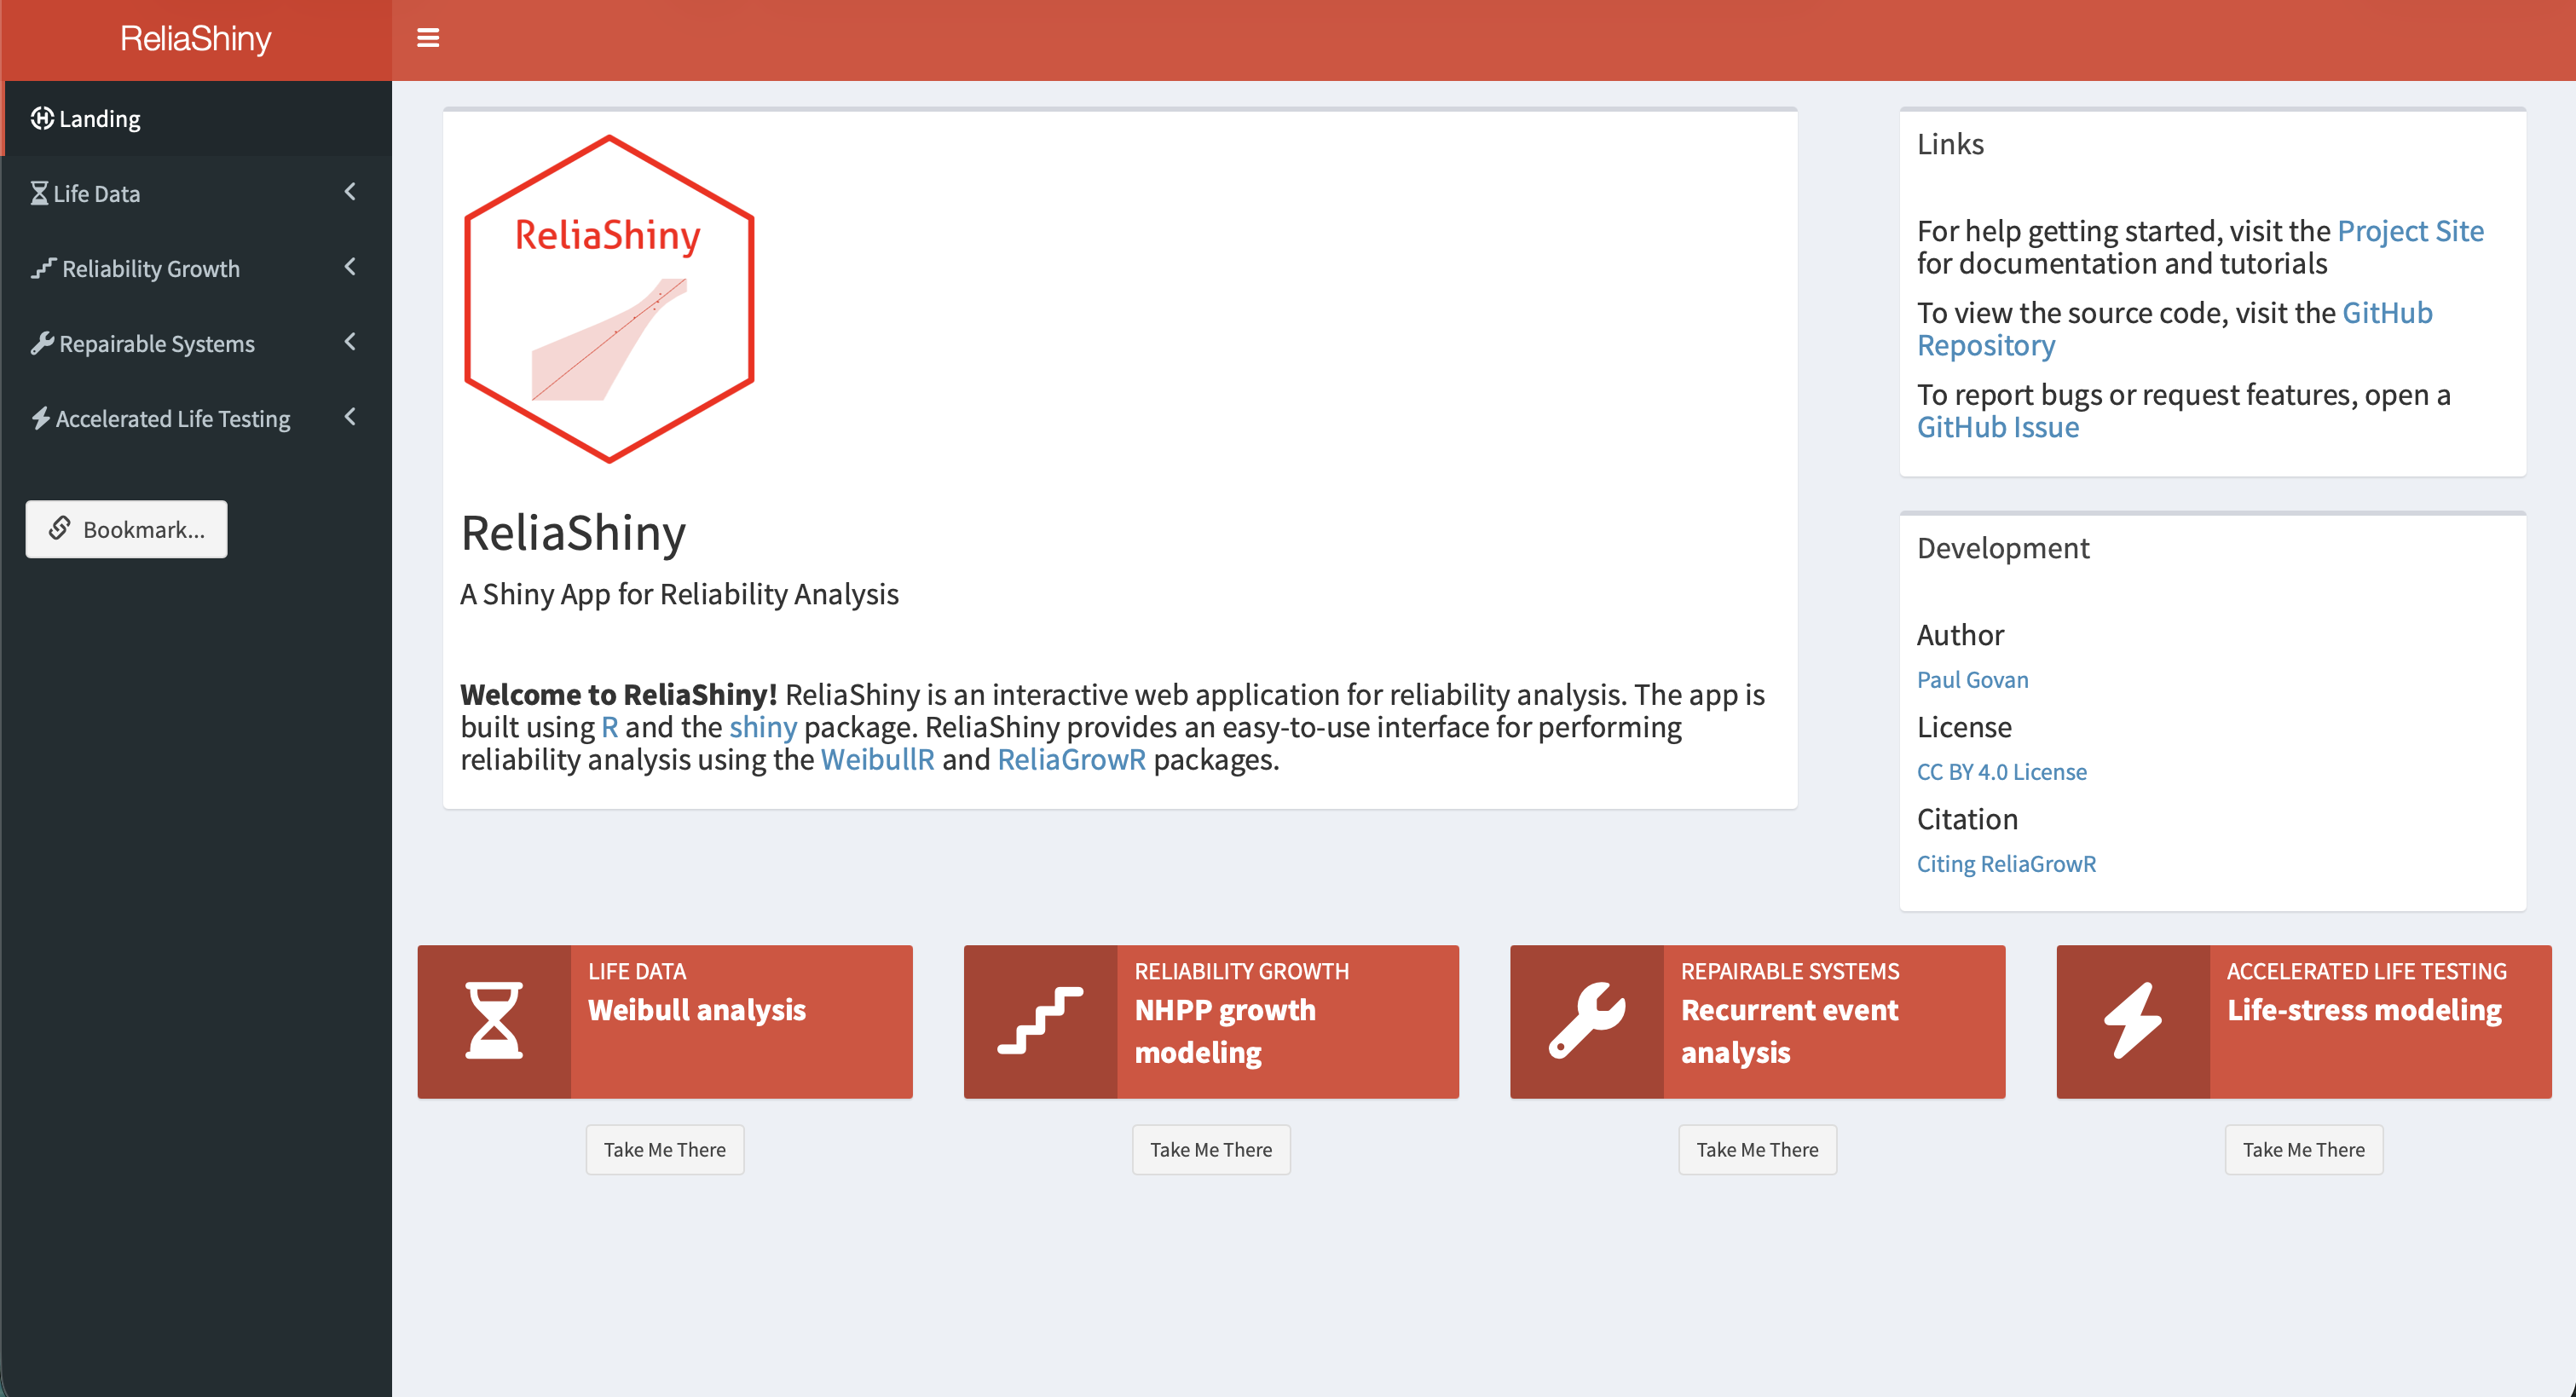
\includegraphics[width=1\linewidth,height=\textheight,keepaspectratio,alt={ReliaShiny web app with a left sidebar listing modules: Life Data Analysis, Reliability Growth, Accelerated Life Testing, and Repairable Systems.}]{images/Landing.png}

}

\caption{ReliaShiny landing page showing the sidebar module list.}

\end{figure}%

{\def\LTcaptype{none} % do not increment counter
\begin{longtable}[]{@{}
  >{\raggedright\arraybackslash}p{(\linewidth - 4\tabcolsep) * \real{0.3333}}
  >{\raggedright\arraybackslash}p{(\linewidth - 4\tabcolsep) * \real{0.3333}}
  >{\raggedright\arraybackslash}p{(\linewidth - 4\tabcolsep) * \real{0.3333}}@{}}
\toprule\noalign{}
\begin{minipage}[b]{\linewidth}\raggedright
Module
\end{minipage} & \begin{minipage}[b]{\linewidth}\raggedright
Corresponding chapter
\end{minipage} & \begin{minipage}[b]{\linewidth}\raggedright
Key capabilities
\end{minipage} \\
\midrule\noalign{}
\endhead
\bottomrule\noalign{}
\endlastfoot
\textbf{Life Data Analysis} & Chapter~\ref{sec-lda} & 2-parameter,
3-parameter Weibull, Weibayes; MRR and MLE; right-censored data \\
\textbf{Reliability Growth} & Chapter~\ref{sec-rt} & Duane and
Crow-AMSAA model fitting; piecewise NHPP \\
\textbf{Accelerated Life Testing} & Chapter~\ref{sec-alt} & Arrhenius
and Power Law models; relationship plots \\
\textbf{Repairable Systems} & Chapter~\ref{sec-rs} & Power Law Process
(NHPP); MCF; fleet exposure \\
\end{longtable}
}

Each module follows the same three-step workflow:

\begin{enumerate}
\def\labelenumi{\arabic{enumi}.}
\tightlist
\item
  \textbf{Input}: enter or upload your data using form fields, tables,
  or file uploads.
\item
  \textbf{Analyze}: click \textbf{Run} to fit the model.
\item
  \textbf{Output}: view plots, parameter estimates, and summary
  statistics; download results.
\end{enumerate}

\section{Module Walkthroughs}\label{module-walkthroughs}

\subsection{Life Data Analysis Module}\label{life-data-analysis-module}

The LDA module fits Weibull models and generates probability and contour
plots. The app includes a preloaded \textbf{Time-to-Failure} dataset so
you can explore the workflow immediately without uploading data.

\begin{figure}[H]

{\centering 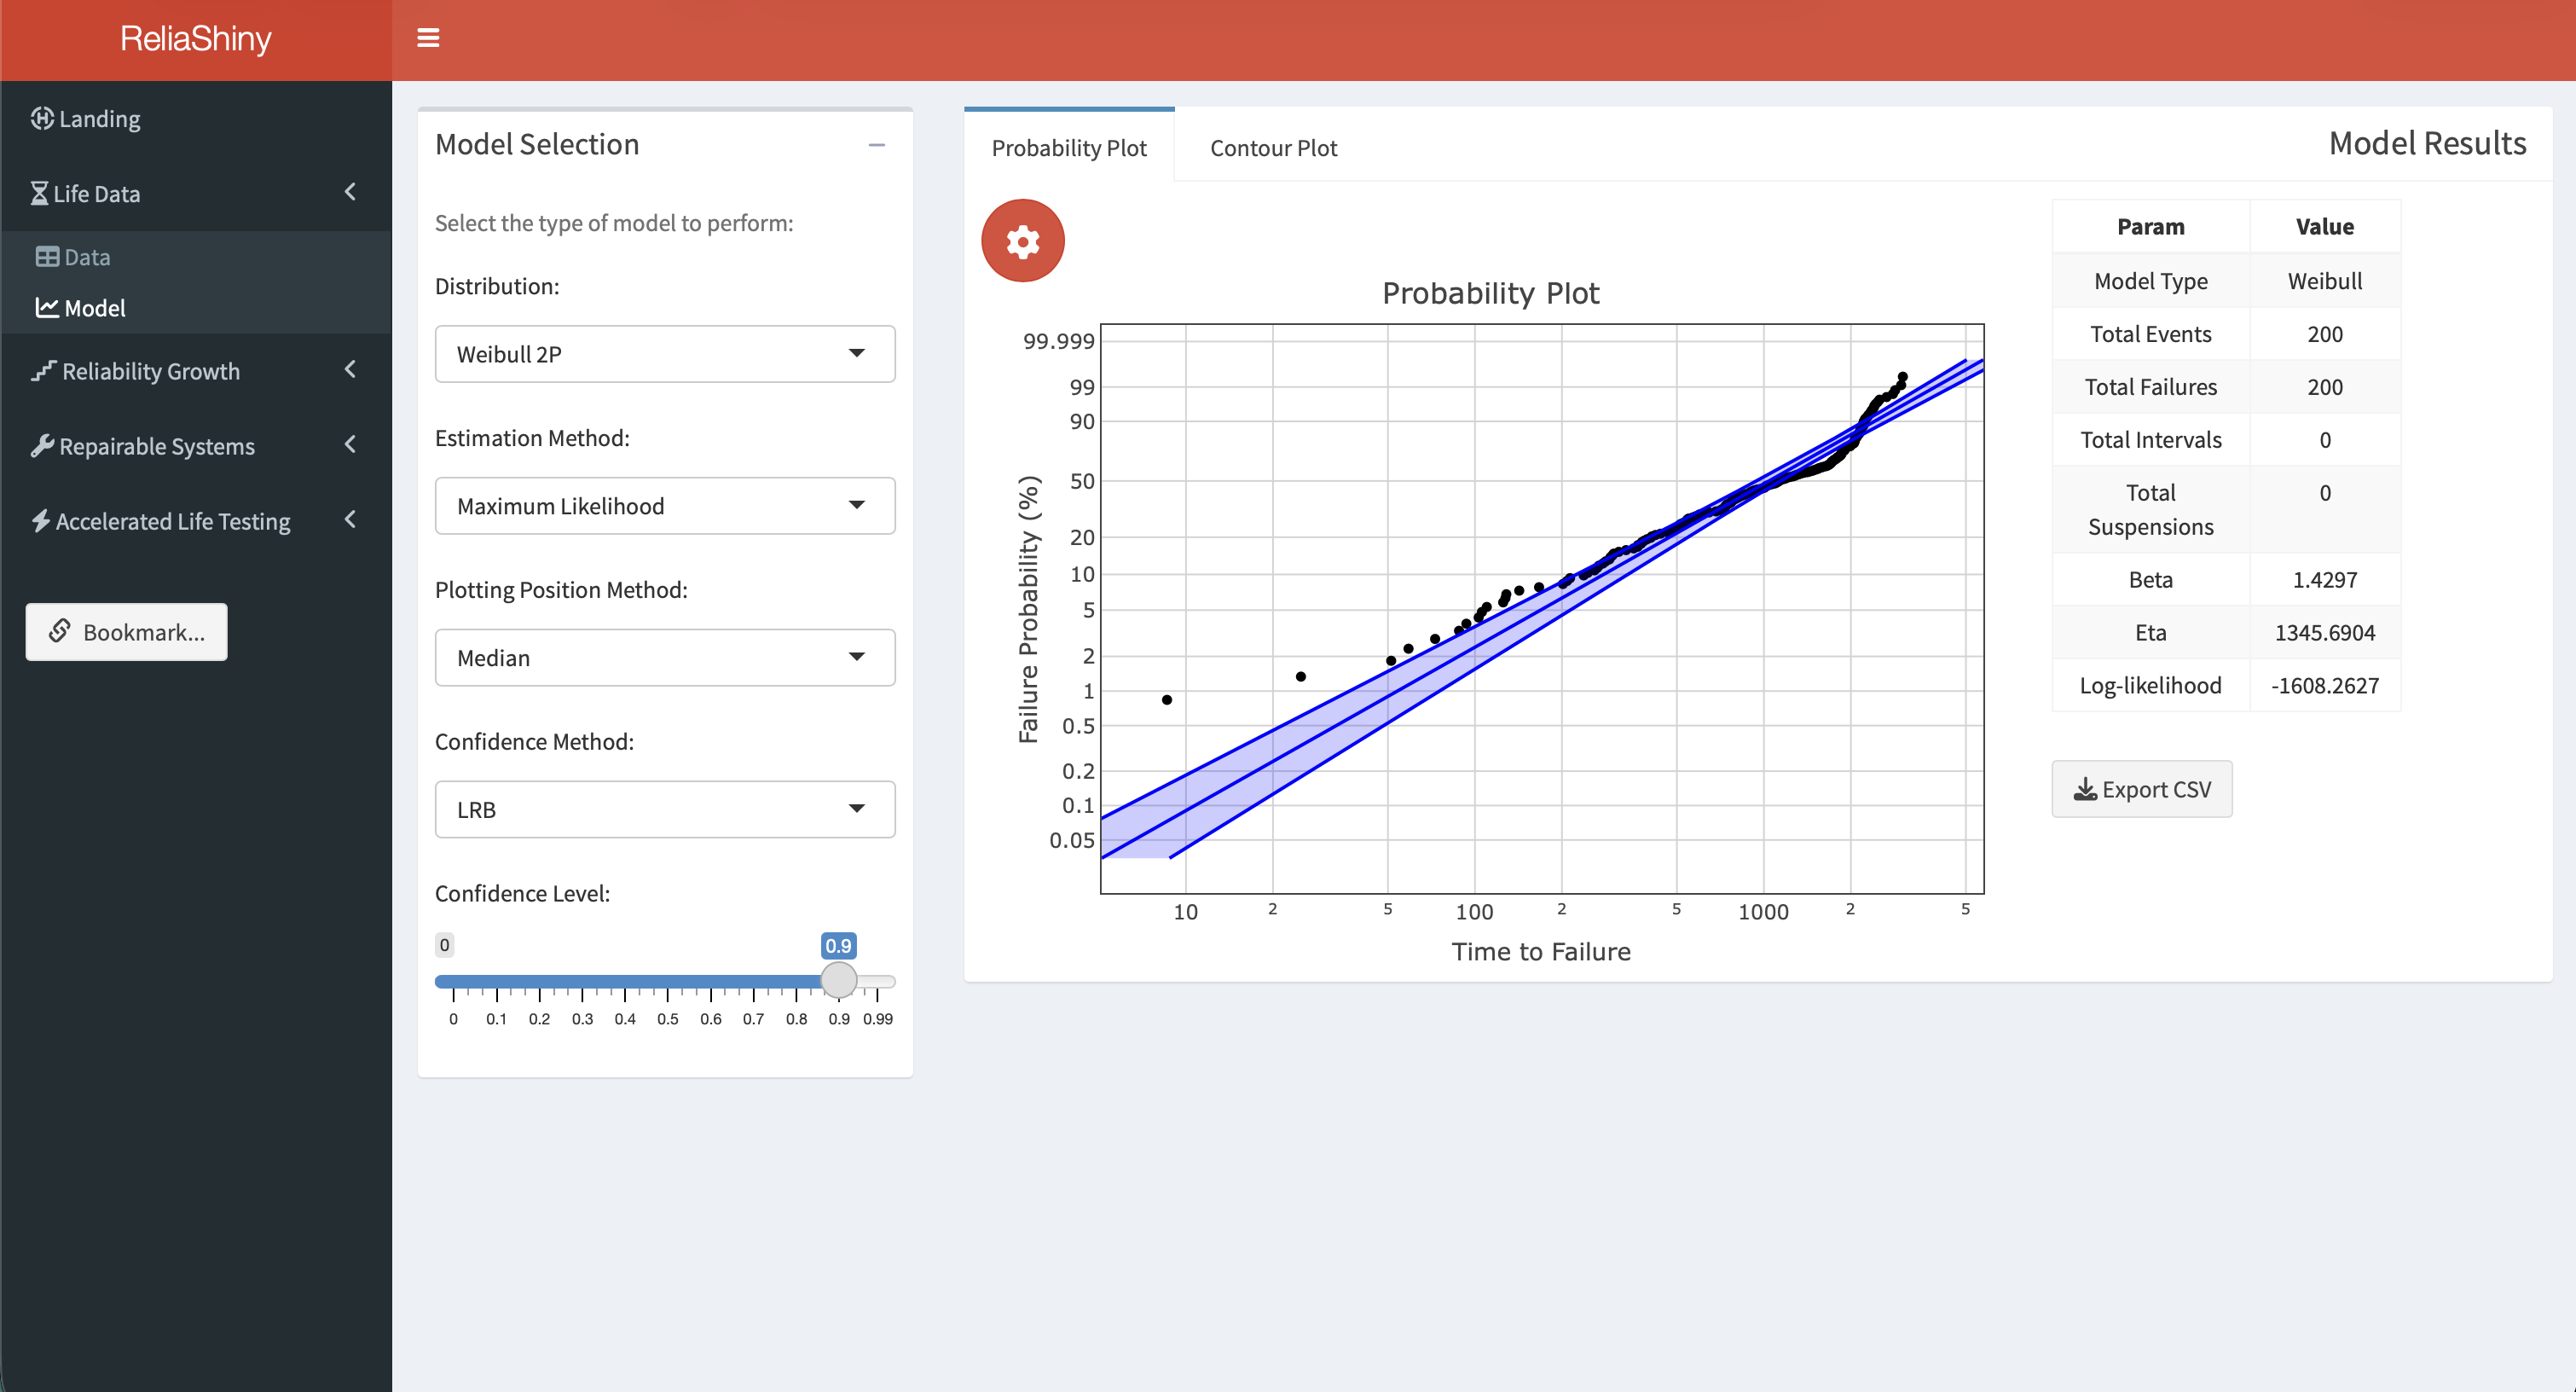
\includegraphics[width=1\linewidth,height=\textheight,keepaspectratio,alt={ReliaShiny Life Data Analysis module with a Weibull probability plot in the main panel and parameter estimates in the sidebar.}]{images/ProbPlot.png}

}

\caption{LDA module showing a fitted Weibull probability plot.}

\end{figure}%

\textbf{Workflow:}

\begin{enumerate}
\def\labelenumi{\arabic{enumi}.}
\tightlist
\item
  Select the \emph{Life Data Analysis} tab in the sidebar.
\item
  Navigate to the \textbf{Data} sub-menu. The preloaded
  \emph{Time-to-Failure} dataset is already loaded; explore additional
  options for data arrangement or upload your own CSV with columns
  \texttt{time} and \texttt{event} (1 = failure, 0 = suspension).
\item
  Navigate to the \textbf{Model} sub-menu. Select the distribution
  (2-parameter Weibull by default) and estimation method (MRR or MLE).
\item
  Click \textbf{Fit Model}. The \textbf{Probability Plot} appears in the
  main panel, with \(\hat{\beta}\), \(\hat{\eta}\), and the
  Anderson-Darling statistic.
\item
  Switch to the \textbf{Contour Plot} tab for an interactive likelihood
  ratio contour showing the joint confidence region for \(\hat{\beta}\)
  and \(\hat{\eta}\).
\item
  Click \textbf{Download Plot} to save the current chart as a PNG.
\end{enumerate}

\textbf{CSV format for upload:}

\begin{verbatim}
time,event
30,1
49,1
82,1
90,1
96,1
100,0
45,0
10,0
\end{verbatim}

A \texttt{0} in the \texttt{event} column marks a suspension
(right-censored observation).

See the
\href{https://paulgovan.github.io/ReliaShiny/articles/LDA.html}{Life
Data Analysis article} for a full walkthrough.

\subsection{Reliability Growth Module}\label{reliability-growth-module}

The Reliability Growth module fits Crow-AMSAA and Duane reliability
growth models. The app includes a preloaded \textbf{Simple Data} dataset
for immediate exploration.

\begin{figure}[H]

{\centering 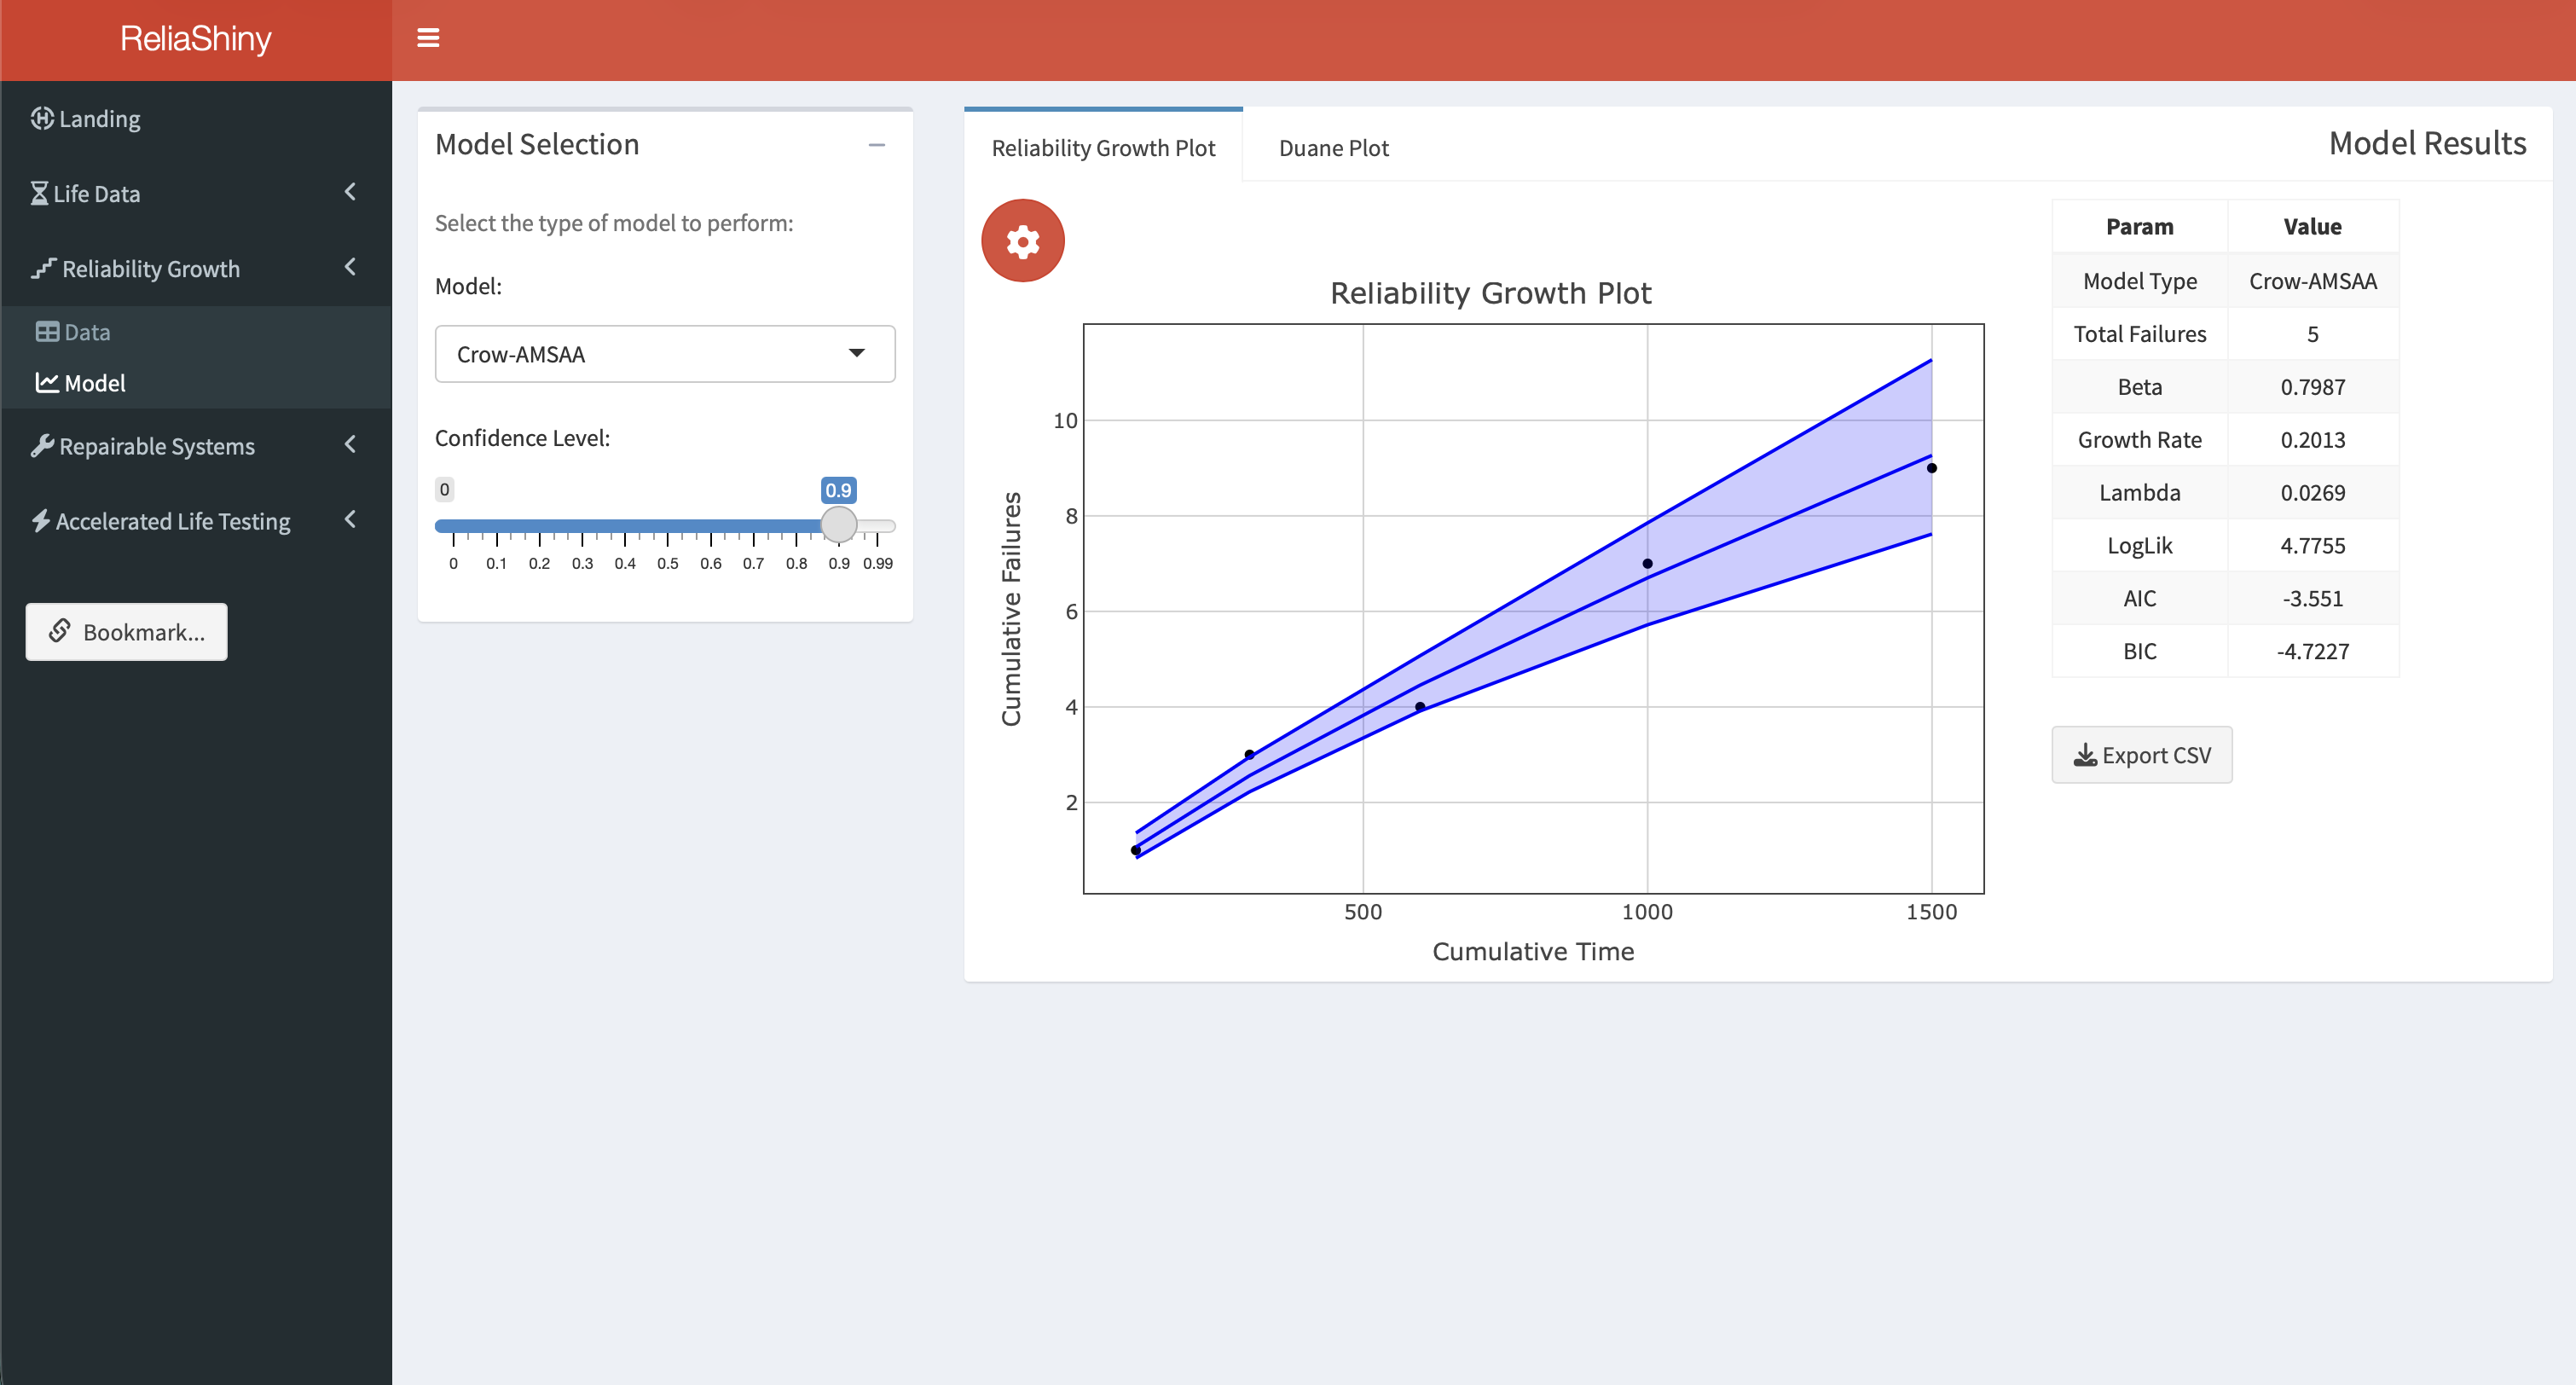
\includegraphics[width=1\linewidth,height=\textheight,keepaspectratio,alt={ReliaShiny Reliability Growth module displaying a Crow-AMSAA cumulative failures plot with fitted model curve.}]{images/GrowthPlot.png}

}

\caption{Reliability Growth module showing a fitted Crow-AMSAA
cumulative failures plot.}

\end{figure}%

\textbf{Workflow:}

\begin{enumerate}
\def\labelenumi{\arabic{enumi}.}
\tightlist
\item
  Select \emph{Reliability Growth} in the sidebar.
\item
  Navigate to the \textbf{Data} sub-menu. The preloaded \emph{Simple
  Data} dataset is loaded; designate the \textbf{failures} column as the
  failure indicator, or upload your own data.
\item
  Navigate to the \textbf{Model} sub-menu.
\item
  Click \textbf{Fit}. The \textbf{Reliability Growth Plot} (Crow-AMSAA
  cumulative failures) appears with the fitted curve and
  \(\hat{\beta}\).
\item
  Switch to the \textbf{Duane Plot} tab to view the log-log cumulative
  MTBF plot for the same data.
\end{enumerate}

See the
\href{https://paulgovan.github.io/ReliaShiny/articles/RGA.html}{Reliability
Growth Analysis article} for a full walkthrough.

\subsection{Accelerated Life Testing
Module}\label{accelerated-life-testing-module}

The ALT module fits Arrhenius and Power Law acceleration models using
the \texttt{WeibullR.ALT} package (see Chapter~\ref{sec-alt}). The app
includes the preloaded \textbf{Nelson Data} dataset.

\begin{figure}[H]

{\centering 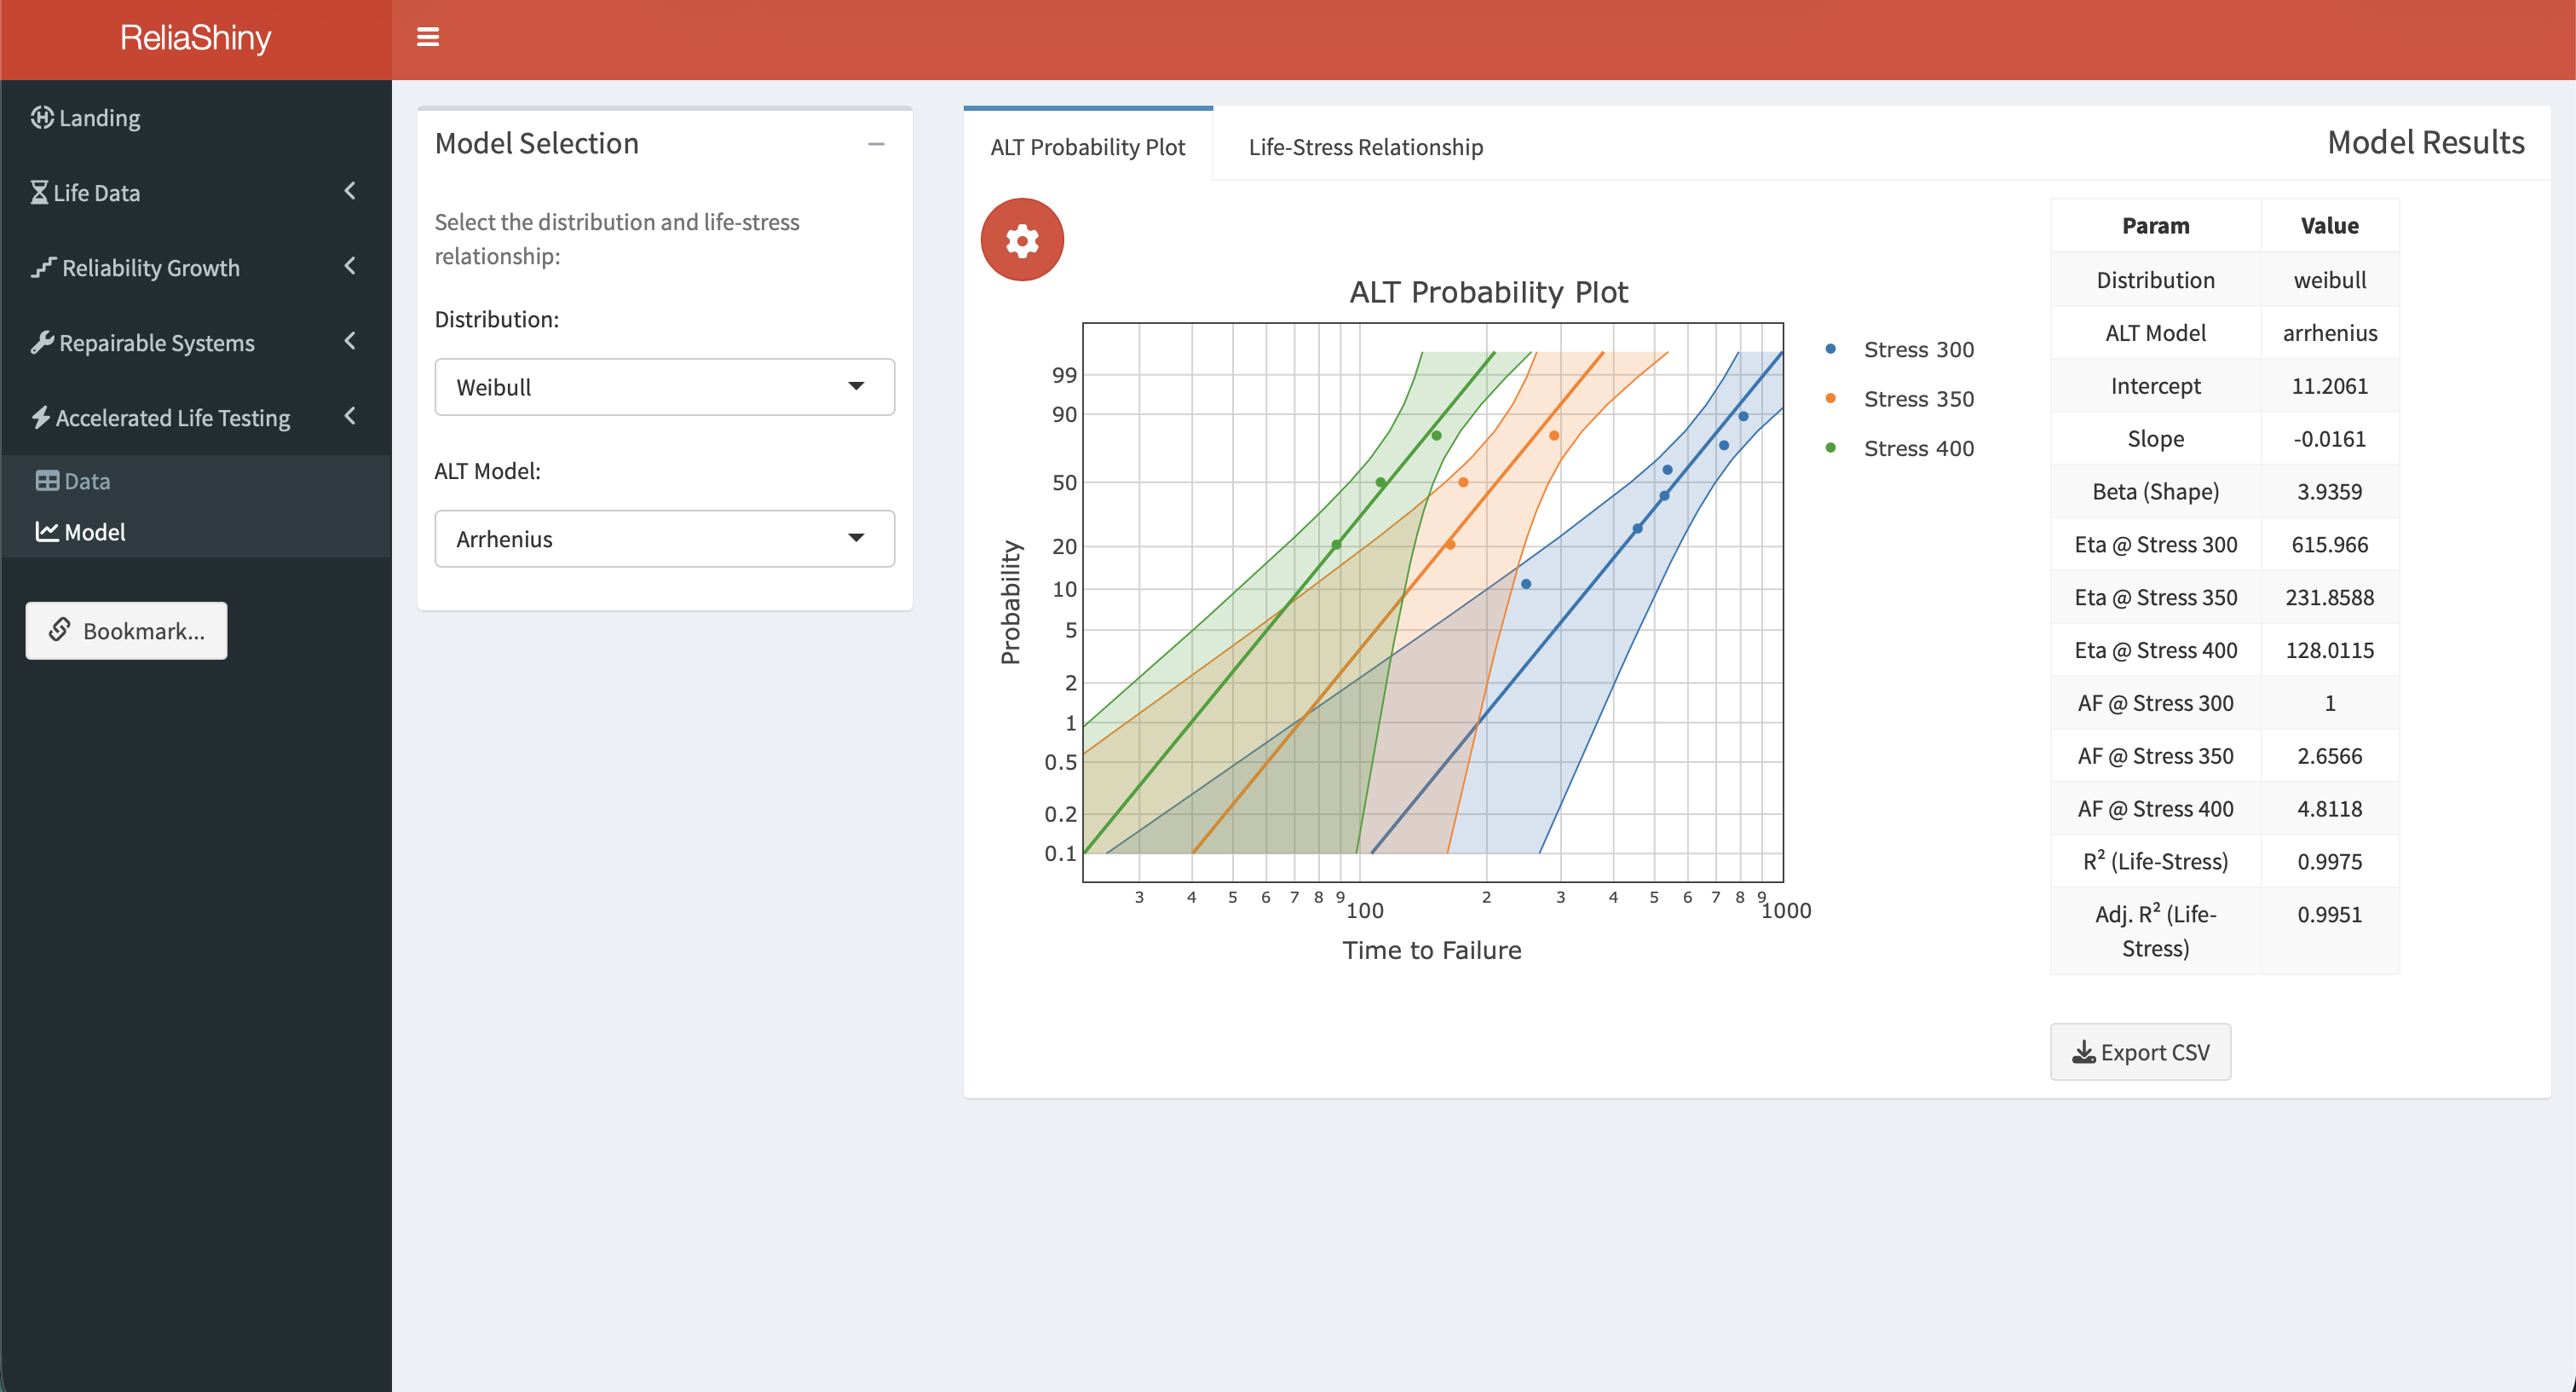
\includegraphics[width=1\linewidth,height=\textheight,keepaspectratio,alt={ReliaShiny Accelerated Life Testing module showing an ALT probability plot with stress-level curves and a life-stress relationship plot.}]{images/ALTPlot.png}

}

\caption{ALT module showing a probability plot and life-stress
relationship.}

\end{figure}%

\textbf{Workflow:}

\begin{enumerate}
\def\labelenumi{\arabic{enumi}.}
\tightlist
\item
  Select \emph{Accelerated Life Testing} in the sidebar.
\item
  Navigate to the \textbf{Data} sub-menu. The preloaded \emph{Nelson
  Data} is already loaded. Map the columns: select the \textbf{Stress
  Level}, \textbf{Time to Failure}, and \textbf{Event Indicator} columns
  from the dropdowns.
\item
  Navigate to the \textbf{Model} sub-menu. Choose the acceleration model
  (\textbf{Arrhenius} for temperature, \textbf{Power Law} for
  voltage/mechanical stress) and distribution (Weibull or Lognormal).
\item
  Click \textbf{Fit ALT Model}. The \textbf{ALT Probability Plot}
  appears, with one curve per stress level.
\item
  Switch to the \textbf{Life-Stress Relationship} tab to view how
  predicted life varies across the stress range, with percentile lines
  (P10, P63.2, P90).
\end{enumerate}

See the
\href{https://paulgovan.github.io/ReliaShiny/articles/ALT.html}{Accelerated
Life Testing article} for a full walkthrough.

\subsection{Repairable Systems Module}\label{repairable-systems-module}

The Repairable Systems module fits the Power Law Process (Crow-AMSAA)
and computes the MCF and exposure for fleet data. The app includes a
preloaded \textbf{Simple Data Set}.

\begin{figure}[H]

{\centering 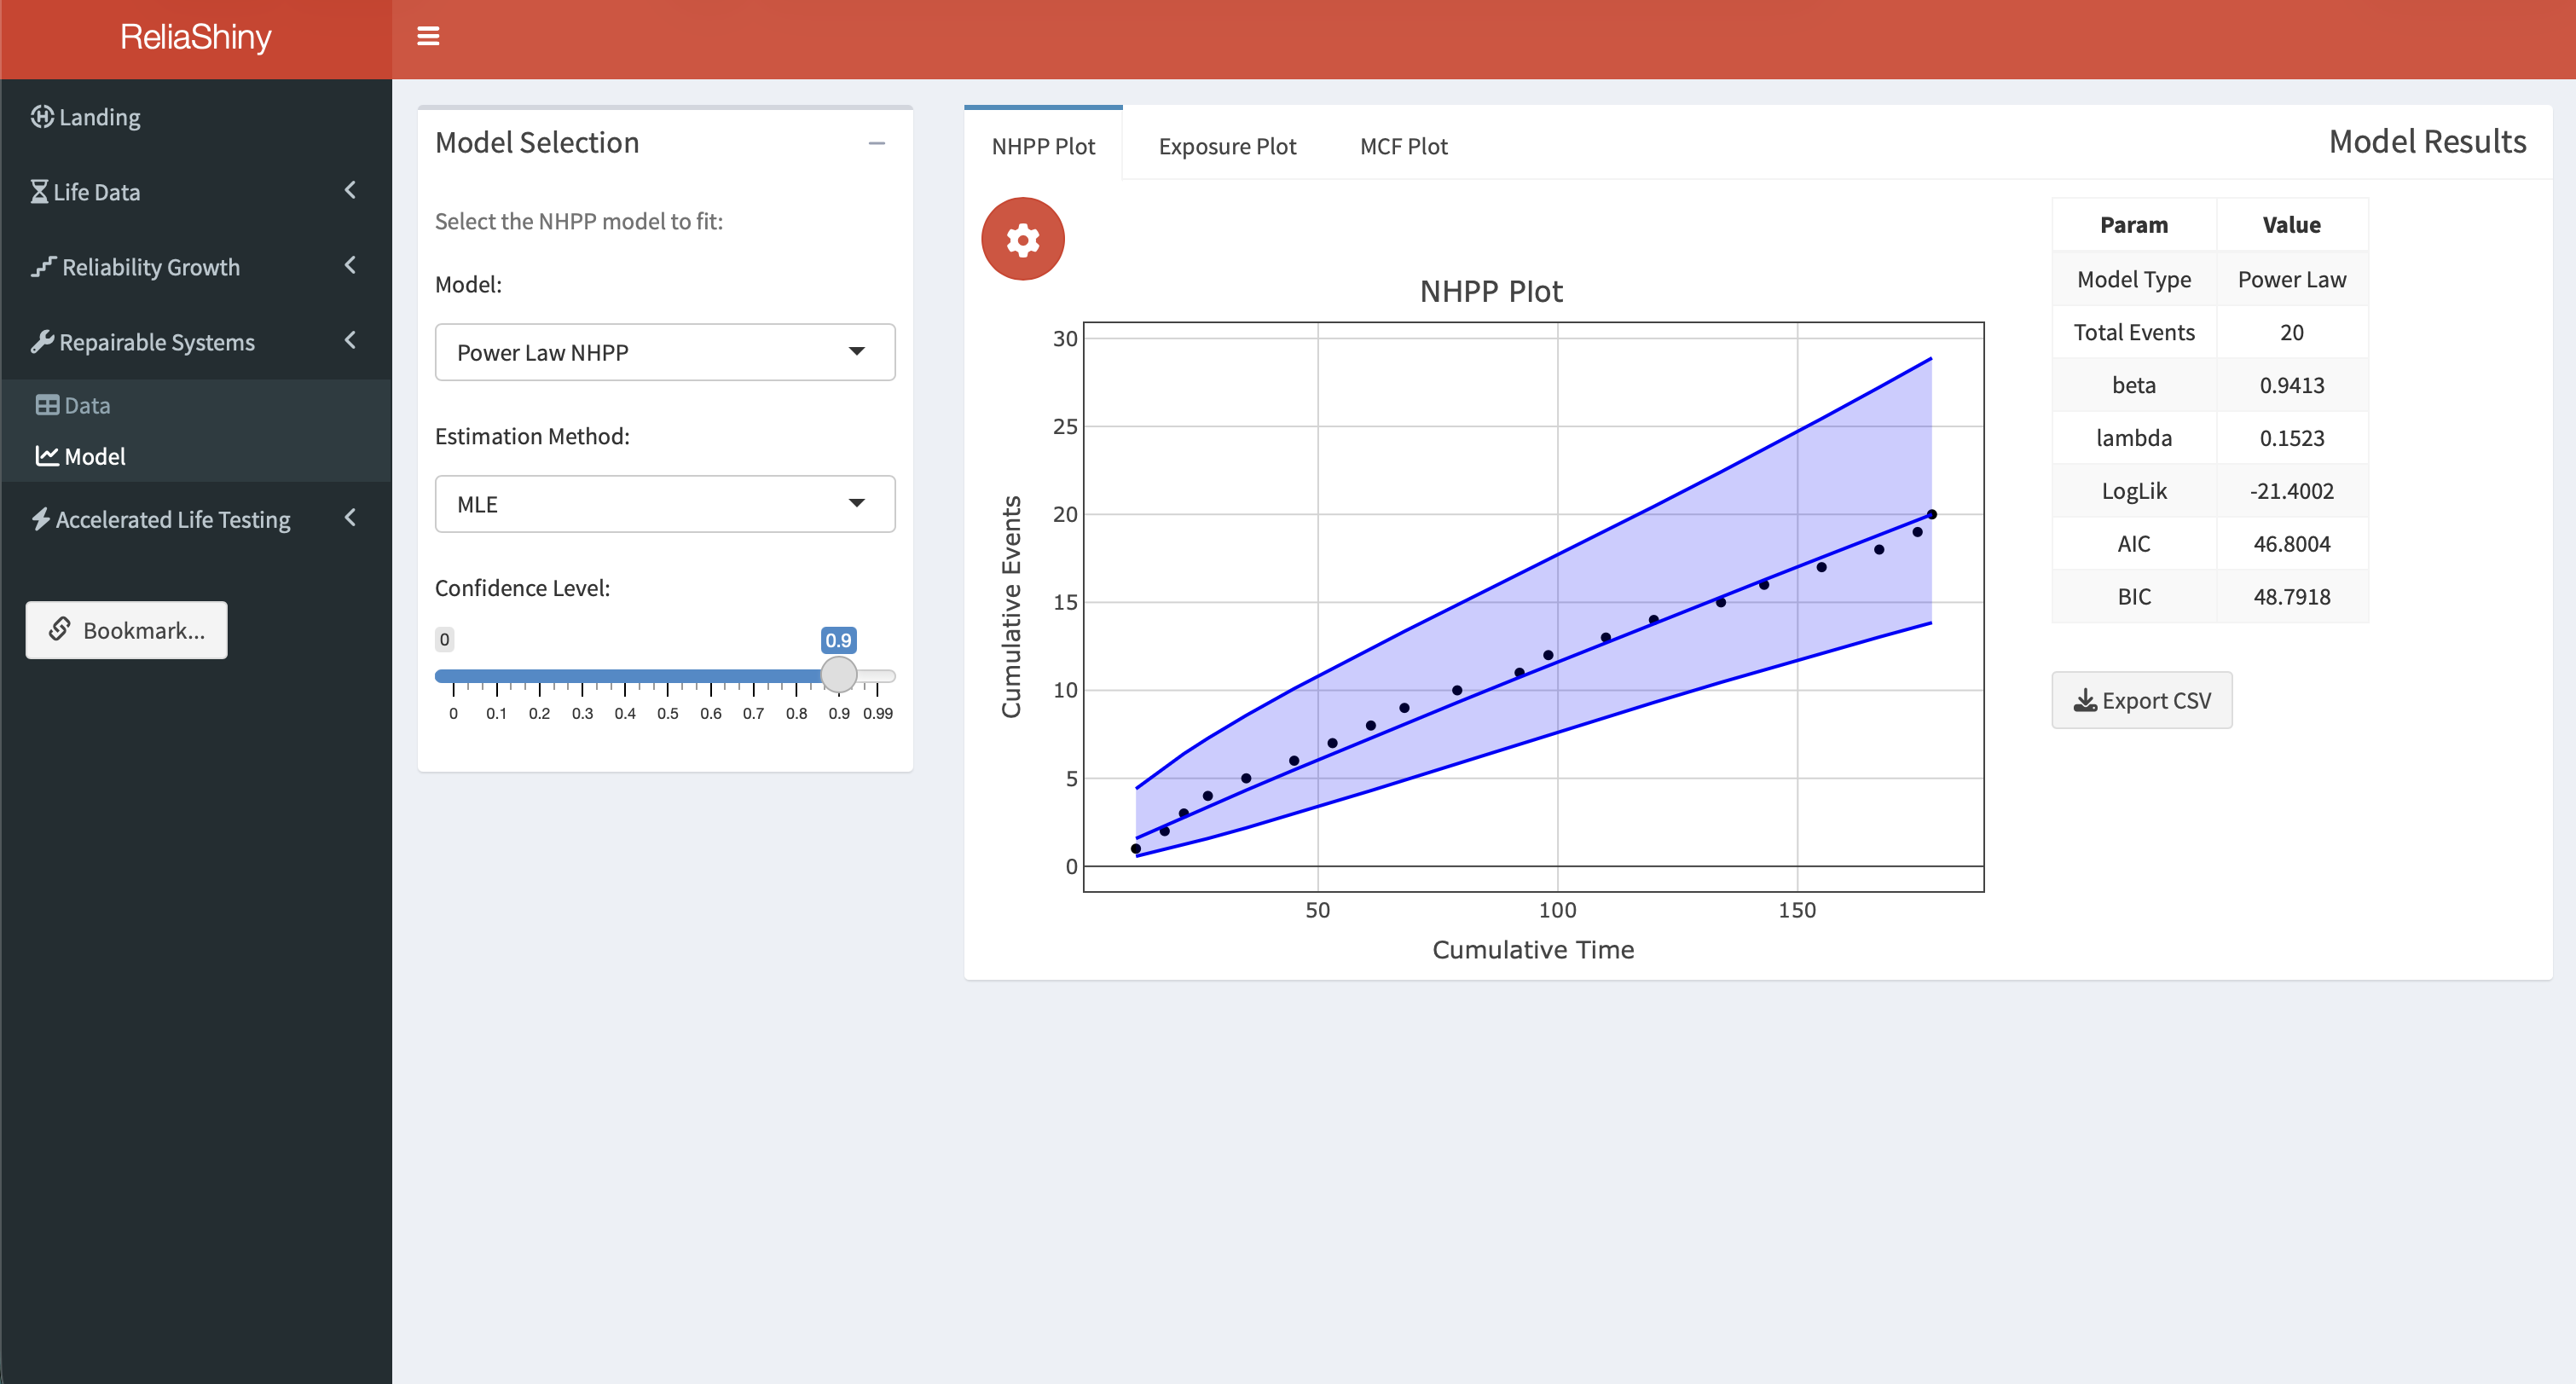
\includegraphics[width=1\linewidth,height=\textheight,keepaspectratio,alt={ReliaShiny Repairable Systems module displaying an MCF cumulative failures curve with confidence bounds for a fleet of systems.}]{images/RepairablePlot.png}

}

\caption{Repairable Systems module showing a Mean Cumulative Function
plot.}

\end{figure}%

\textbf{Workflow:}

\begin{enumerate}
\def\labelenumi{\arabic{enumi}.}
\tightlist
\item
  Select \emph{Repairable Systems} in the sidebar.
\item
  Navigate to the \textbf{Data} sub-menu. The preloaded \emph{Simple
  Data Set} is loaded; map the \textbf{System ID}, \textbf{Event Time},
  and \textbf{Event Indicator} columns, or upload your own fleet data
  with columns \texttt{id}, \texttt{time}, and \texttt{event}.
\item
  Navigate to the \textbf{Model} sub-menu.
\item
  Click \textbf{Analyze}. Three plots are produced:

  \begin{itemize}
  \tightlist
  \item
    \textbf{NHPP Plot}: Crow-AMSAA Power Law fit with cumulative
    failures curve and \(\hat{\beta}\), \(\hat{\lambda}\).
  \item
    \textbf{Exposure Plot}: fleet-level event rate as a function of
    operating time.
  \item
    \textbf{MCF Plot}: non-parametric Mean Cumulative Function with
    confidence bounds.
  \end{itemize}
\end{enumerate}

\textbf{Example CSV format:}

\begin{verbatim}
id,time,event
1,310,1
1,850,1
1,1620,1
2,420,1
2,1050,1
2,3000,0
\end{verbatim}

The last row for system 2 (\texttt{event\ =\ 0}) indicates that system 2
was observed until hour 3,000 without a third failure.

See the
\href{https://paulgovan.github.io/ReliaShiny/articles/RS.html}{Repairable
Systems Analysis article} for a full walkthrough.

\section{Data Upload Tips}\label{data-upload-tips}

\begin{itemize}
\tightlist
\item
  \textbf{CSV files}: core column names (\texttt{time}, \texttt{event},
  \texttt{id}, \texttt{qty}) are case-sensitive and must be
  \textbf{lowercase}. Stress column names (e.g., \texttt{TempC},
  \texttt{Voltage}) may use any valid R name; they are selected in the
  app's dropdown.
\item
  \textbf{Missing values}: rows with \texttt{NA} in the \texttt{time}
  column are automatically excluded.
\item
  \textbf{Large datasets}: the app handles datasets up to
  \textasciitilde10,000 rows without performance issues.
\item
  \textbf{Units}: ReliaShiny is unit-agnostic; use hours, years, cycles,
  or any consistent unit. Label your outputs accordingly.
\end{itemize}

\section{Downloading Results}\label{downloading-results}

Every module provides download buttons for:

\begin{itemize}
\tightlist
\item
  \textbf{Plot PNG}: the current chart at screen resolution.
\item
  \textbf{Results CSV}: parameter estimates and summary statistics in
  tabular form.
\item
  \textbf{Report HTML}: a self-contained report combining the inputs,
  plot, and results (available in LDA and RT modules).
\end{itemize}

\section{When to Use ReliaShiny vs Scripted
R}\label{when-to-use-reliashiny-vs-scripted-r}

{\def\LTcaptype{none} % do not increment counter
\begin{longtable}[]{@{}lcc@{}}
\toprule\noalign{}
Situation & ReliaShiny & Scripted R \\
\midrule\noalign{}
\endhead
\bottomrule\noalign{}
\endlastfoot
Quick one-off analysis & ✅ & \\
Teaching / demonstration & ✅ & \\
Sharing with non-R users & ✅ & \\
Automating repeated analyses & & ✅ \\
Custom plots and formatting & & ✅ \\
Reproducible research / version control & & ✅ \\
Embedding results in a Quarto book & & ✅ \\
Large batch processing & & ✅ \\
\end{longtable}
}

ReliaShiny excels at rapid exploration, prototyping, and sharing results
with stakeholders who do not use R. For production workflows, automated
pipelines, and fully reproducible analyses, scripted R with the
underlying packages (WeibullR, ReliaGrowR, WeibullR.ALT) gives more
control.

\section{Getting Help}\label{getting-help-1}

Within the app, click the \textbf{?} icon on any panel for a tooltip
explaining the inputs and outputs for that module.

From R:

\begin{Shaded}
\begin{Highlighting}[]
\FunctionTok{help}\NormalTok{(}\AttributeTok{package =} \StringTok{"ReliaShiny"}\NormalTok{)}
\end{Highlighting}
\end{Shaded}

Additional resources:

\begin{itemize}
\tightlist
\item
  CRAN page: \url{https://CRAN.R-project.org/package=ReliaShiny}
\item
  Articles and walkthroughs:
  \url{https://paulgovan.github.io/ReliaShiny/}
\end{itemize}

\section{Summary}\label{summary-7}

ReliaShiny provides a point-and-click interface to the ReliaLearnR
analysis ecosystem, covering life data analysis, reliability growth,
accelerated life testing, and repairable systems, with no R coding
required. Install it with \texttt{install.packages("ReliaShiny")} and
launch it with \texttt{ReliaShiny()}. Use it for rapid exploration,
stakeholder demonstrations, and sharing results; switch to scripted R
for reproducibility, automation, and custom outputs.

\bookmarksetup{startatroot}

\chapter{AI-Assisted Reliability Analysis with MCP}\label{sec-mcp}

\section{Introduction}\label{introduction-8}

All of the analyses in this book require writing R code or navigating a
Shiny app. \textbf{Model Context Protocol (MCP)} opens a third path:
letting an AI assistant call your R functions directly during a
conversation, so you can describe what you want in plain language and
the AI runs the analysis, interprets the results, and generates the
plots.

MCP is an open standard that defines how an AI assistant discovers and
calls external tools --- in the same way a web browser calls REST APIs.
Reliability workflows are a natural fit: fitting a growth model,
predicting future failures, computing a fleet MCF, and saving an
interactive plot are all discrete, well-defined operations that map
cleanly to MCP tools.

This chapter shows how to expose \texttt{ReliaGrowR} (Govan 2024) and
\texttt{ReliaPlotR} (Govan 2023a) as an MCP server so that Claude
Desktop, Claude Code, or any other MCP-compatible client can run
reliability analyses on demand.

\section{Prerequisites}\label{prerequisites}

Install the MCP infrastructure packages. \texttt{ellmer} (Wickham and
Cheng 2025) provides the \texttt{tool()} constructor; \texttt{mcptools}
(Posit PBC 2025) provides the server transport:

\begin{Shaded}
\begin{Highlighting}[]
\FunctionTok{install.packages}\NormalTok{(}\FunctionTok{c}\NormalTok{(}\StringTok{"ellmer"}\NormalTok{, }\StringTok{"mcptools"}\NormalTok{))}
\end{Highlighting}
\end{Shaded}

Ensure the reliability packages are also installed:

\begin{Shaded}
\begin{Highlighting}[]
\FunctionTok{install.packages}\NormalTok{(}\FunctionTok{c}\NormalTok{(}\StringTok{"ReliaGrowR"}\NormalTok{, }\StringTok{"ReliaPlotR"}\NormalTok{, }\StringTok{"htmlwidgets"}\NormalTok{))}
\end{Highlighting}
\end{Shaded}

\section{MCP Tools for ReliaGrowR}\label{mcp-tools-for-reliagrowr}

The \texttt{reliagrow\_mcp\_tools()} function below returns a named list
of \texttt{ellmer::tool()} objects. Each tool is a thin wrapper: it
accepts plain-text inputs (times and failures as comma-separated
strings), calls the underlying \texttt{ReliaGrowR} function, extracts
the key scalar results, and returns a plain list that the AI receives as
JSON.

\begin{Shaded}
\begin{Highlighting}[]
\FunctionTok{library}\NormalTok{(ellmer)}
\FunctionTok{library}\NormalTok{(ReliaGrowR)}

\NormalTok{reliagrow\_mcp\_tools }\OtherTok{\textless{}{-}} \ControlFlowTok{function}\NormalTok{() \{}

\NormalTok{  parse\_vec }\OtherTok{\textless{}{-}} \ControlFlowTok{function}\NormalTok{(x) }\FunctionTok{as.numeric}\NormalTok{(}\FunctionTok{strsplit}\NormalTok{(}\FunctionTok{trimws}\NormalTok{(x), }\StringTok{"}\SpecialCharTok{\textbackslash{}\textbackslash{}}\StringTok{s*,}\SpecialCharTok{\textbackslash{}\textbackslash{}}\StringTok{s*"}\NormalTok{)[[}\DecValTok{1}\NormalTok{]])}

  \FunctionTok{list}\NormalTok{(}

    \AttributeTok{fit\_duane =} \FunctionTok{tool}\NormalTok{(}
      \AttributeTok{.name        =} \StringTok{"fit\_duane"}\NormalTok{,}
      \AttributeTok{.description =} \StringTok{"Fit a Duane reliability growth model to cumulative failure data.}
\StringTok{                      Returns the growth slope (beta), scale parameter (K), and}
\StringTok{                      cumulative MTBF at the last observation."}\NormalTok{,}
      \AttributeTok{times    =} \FunctionTok{type\_string}\NormalTok{(}\StringTok{"Comma{-}separated cumulative times (e.g. \textquotesingle{}100,200,300\textquotesingle{})"}\NormalTok{),}
      \AttributeTok{failures =} \FunctionTok{type\_string}\NormalTok{(}\StringTok{"Comma{-}separated cumulative failure counts (e.g. \textquotesingle{}1,2,1\textquotesingle{})"}\NormalTok{),}
      \ControlFlowTok{function}\NormalTok{(times, failures) \{}
\NormalTok{        t }\OtherTok{\textless{}{-}} \FunctionTok{parse\_vec}\NormalTok{(times)}
\NormalTok{        f }\OtherTok{\textless{}{-}} \FunctionTok{parse\_vec}\NormalTok{(failures)}
\NormalTok{        fit }\OtherTok{\textless{}{-}} \FunctionTok{duane}\NormalTok{(t, f)}
        \FunctionTok{list}\NormalTok{(}
          \AttributeTok{beta  =} \FunctionTok{round}\NormalTok{(fit}\SpecialCharTok{$}\NormalTok{beta, }\DecValTok{4}\NormalTok{),}
          \AttributeTok{K     =} \FunctionTok{round}\NormalTok{(fit}\SpecialCharTok{$}\NormalTok{K, }\DecValTok{4}\NormalTok{),}
          \AttributeTok{cmtbf =} \FunctionTok{round}\NormalTok{(fit}\SpecialCharTok{$}\NormalTok{K }\SpecialCharTok{*} \FunctionTok{max}\NormalTok{(t)}\SpecialCharTok{\^{}}\NormalTok{(fit}\SpecialCharTok{$}\NormalTok{beta }\SpecialCharTok{{-}} \DecValTok{1}\NormalTok{), }\DecValTok{2}\NormalTok{)}
\NormalTok{        )}
\NormalTok{      \}}
\NormalTok{    ),}

    \AttributeTok{fit\_crow\_amsaa =} \FunctionTok{tool}\NormalTok{(}
      \AttributeTok{.name        =} \StringTok{"fit\_crow\_amsaa"}\NormalTok{,}
      \AttributeTok{.description =} \StringTok{"Fit a Crow{-}AMSAA (NHPP Power Law) reliability growth model.}
\StringTok{                      Returns beta (shape) and lambda (scale). Beta \textless{} 1 means}
\StringTok{                      reliability is improving; beta \textgreater{} 1 means worsening."}\NormalTok{,}
      \AttributeTok{times    =} \FunctionTok{type\_string}\NormalTok{(}\StringTok{"Comma{-}separated cumulative times"}\NormalTok{),}
      \AttributeTok{failures =} \FunctionTok{type\_string}\NormalTok{(}\StringTok{"Comma{-}separated cumulative failure counts"}\NormalTok{),}
      \ControlFlowTok{function}\NormalTok{(times, failures) \{}
\NormalTok{        t }\OtherTok{\textless{}{-}} \FunctionTok{parse\_vec}\NormalTok{(times)}
\NormalTok{        f }\OtherTok{\textless{}{-}} \FunctionTok{parse\_vec}\NormalTok{(failures)}
\NormalTok{        fit }\OtherTok{\textless{}{-}} \FunctionTok{rga}\NormalTok{(t, f, }\AttributeTok{model\_type =} \StringTok{"Crow{-}AMSAA"}\NormalTok{)}
        \FunctionTok{list}\NormalTok{(}
          \AttributeTok{beta   =} \FunctionTok{round}\NormalTok{(fit}\SpecialCharTok{$}\NormalTok{beta, }\DecValTok{4}\NormalTok{),}
          \AttributeTok{lambda =} \FunctionTok{round}\NormalTok{(fit}\SpecialCharTok{$}\NormalTok{lambda, }\DecValTok{6}\NormalTok{)}
\NormalTok{        )}
\NormalTok{      \}}
\NormalTok{    ),}

    \AttributeTok{fit\_piecewise\_nhpp =} \FunctionTok{tool}\NormalTok{(}
      \AttributeTok{.name        =} \StringTok{"fit\_piecewise\_nhpp"}\NormalTok{,}
      \AttributeTok{.description =} \StringTok{"Fit a piecewise Crow{-}AMSAA model with an optional known breakpoint.}
\StringTok{                      If no breakpoint is supplied, the change point is detected automatically.}
\StringTok{                      Returns per{-}segment beta and lambda values."}\NormalTok{,}
      \AttributeTok{times     =} \FunctionTok{type\_string}\NormalTok{(}\StringTok{"Comma{-}separated cumulative times"}\NormalTok{),}
      \AttributeTok{failures  =} \FunctionTok{type\_string}\NormalTok{(}\StringTok{"Comma{-}separated cumulative failure counts"}\NormalTok{),}
      \AttributeTok{breakpoint =} \FunctionTok{type\_string}\NormalTok{(}\StringTok{"Optional breakpoint time, or empty string for auto{-}detection"}\NormalTok{),}
      \ControlFlowTok{function}\NormalTok{(times, failures, }\AttributeTok{breakpoint =} \StringTok{""}\NormalTok{) \{}
\NormalTok{        t  }\OtherTok{\textless{}{-}} \FunctionTok{parse\_vec}\NormalTok{(times)}
\NormalTok{        f  }\OtherTok{\textless{}{-}} \FunctionTok{parse\_vec}\NormalTok{(failures)}
\NormalTok{        bp }\OtherTok{\textless{}{-}} \ControlFlowTok{if}\NormalTok{ (}\FunctionTok{nchar}\NormalTok{(}\FunctionTok{trimws}\NormalTok{(breakpoint)) }\SpecialCharTok{==} \DecValTok{0}\NormalTok{) }\ConstantTok{NULL} \ControlFlowTok{else} \FunctionTok{as.numeric}\NormalTok{(breakpoint)}
\NormalTok{        fit }\OtherTok{\textless{}{-}} \ControlFlowTok{if}\NormalTok{ (}\FunctionTok{is.null}\NormalTok{(bp)) \{}
          \FunctionTok{rga}\NormalTok{(t, f, }\AttributeTok{model\_type =} \StringTok{"Piecewise NHPP"}\NormalTok{)}
\NormalTok{        \} }\ControlFlowTok{else}\NormalTok{ \{}
          \FunctionTok{rga}\NormalTok{(t, f, }\AttributeTok{model\_type =} \StringTok{"Piecewise NHPP"}\NormalTok{, }\AttributeTok{breaks =}\NormalTok{ bp)}
\NormalTok{        \}}
        \FunctionTok{list}\NormalTok{(}
          \AttributeTok{segments   =} \FunctionTok{length}\NormalTok{(fit}\SpecialCharTok{$}\NormalTok{beta),}
          \AttributeTok{beta       =} \FunctionTok{round}\NormalTok{(fit}\SpecialCharTok{$}\NormalTok{beta, }\DecValTok{4}\NormalTok{),}
          \AttributeTok{lambda     =} \FunctionTok{round}\NormalTok{(fit}\SpecialCharTok{$}\NormalTok{lambda, }\DecValTok{6}\NormalTok{),}
          \AttributeTok{breakpoints =}\NormalTok{ fit}\SpecialCharTok{$}\NormalTok{breaks}
\NormalTok{        )}
\NormalTok{      \}}
\NormalTok{    ),}

    \AttributeTok{predict\_growth =} \FunctionTok{tool}\NormalTok{(}
      \AttributeTok{.name        =} \StringTok{"predict\_growth"}\NormalTok{,}
      \AttributeTok{.description =} \StringTok{"Predict cumulative failures at future times from a fitted Crow{-}AMSAA model."}\NormalTok{,}
      \AttributeTok{times      =} \FunctionTok{type\_string}\NormalTok{(}\StringTok{"Historical cumulative times used to fit the model"}\NormalTok{),}
      \AttributeTok{failures   =} \FunctionTok{type\_string}\NormalTok{(}\StringTok{"Historical cumulative failure counts"}\NormalTok{),}
      \AttributeTok{pred\_times =} \FunctionTok{type\_string}\NormalTok{(}\StringTok{"Future times to predict at (comma{-}separated)"}\NormalTok{),}
      \ControlFlowTok{function}\NormalTok{(times, failures, pred\_times) \{}
\NormalTok{        t  }\OtherTok{\textless{}{-}} \FunctionTok{parse\_vec}\NormalTok{(times)}
\NormalTok{        f  }\OtherTok{\textless{}{-}} \FunctionTok{parse\_vec}\NormalTok{(failures)}
\NormalTok{        pt }\OtherTok{\textless{}{-}} \FunctionTok{parse\_vec}\NormalTok{(pred\_times)}
\NormalTok{        fit  }\OtherTok{\textless{}{-}} \FunctionTok{rga}\NormalTok{(t, f)}
\NormalTok{        pred }\OtherTok{\textless{}{-}} \FunctionTok{predict\_rga}\NormalTok{(fit, }\AttributeTok{times =}\NormalTok{ pt)}
        \FunctionTok{data.frame}\NormalTok{(}
          \AttributeTok{time               =}\NormalTok{ pt,}
          \AttributeTok{predicted\_failures =} \FunctionTok{round}\NormalTok{(pred}\SpecialCharTok{$}\NormalTok{predicted, }\DecValTok{2}\NormalTok{),}
          \AttributeTok{lower\_95           =} \FunctionTok{round}\NormalTok{(pred}\SpecialCharTok{$}\NormalTok{lower, }\DecValTok{2}\NormalTok{),}
          \AttributeTok{upper\_95           =} \FunctionTok{round}\NormalTok{(pred}\SpecialCharTok{$}\NormalTok{upper, }\DecValTok{2}\NormalTok{)}
\NormalTok{        )}
\NormalTok{      \}}
\NormalTok{    ),}

    \AttributeTok{fit\_nhpp =} \FunctionTok{tool}\NormalTok{(}
      \AttributeTok{.name        =} \StringTok{"fit\_nhpp"}\NormalTok{,}
      \AttributeTok{.description =} \StringTok{"Fit a Crow{-}AMSAA Non{-}Homogeneous Poisson Process (NHPP) to}
\StringTok{                      repairable systems fleet failure times. Returns beta and lambda."}\NormalTok{,}
      \AttributeTok{failure\_times =} \FunctionTok{type\_string}\NormalTok{(}\StringTok{"Comma{-}separated failure times across all systems (pooled)"}\NormalTok{),}
      \ControlFlowTok{function}\NormalTok{(failure\_times) \{}
\NormalTok{        ft  }\OtherTok{\textless{}{-}} \FunctionTok{parse\_vec}\NormalTok{(failure\_times)}
\NormalTok{        fit }\OtherTok{\textless{}{-}} \FunctionTok{nhpp}\NormalTok{(}\AttributeTok{time =}\NormalTok{ ft, }\AttributeTok{event =} \FunctionTok{rep}\NormalTok{(}\DecValTok{1}\NormalTok{L, }\FunctionTok{length}\NormalTok{(ft)))}
        \FunctionTok{list}\NormalTok{(}
          \AttributeTok{beta   =} \FunctionTok{round}\NormalTok{(fit}\SpecialCharTok{$}\NormalTok{beta, }\DecValTok{4}\NormalTok{),}
          \AttributeTok{lambda =} \FunctionTok{round}\NormalTok{(fit}\SpecialCharTok{$}\NormalTok{lambda, }\DecValTok{6}\NormalTok{)}
\NormalTok{        )}
\NormalTok{      \}}
\NormalTok{    ),}

    \AttributeTok{compute\_mcf =} \FunctionTok{tool}\NormalTok{(}
      \AttributeTok{.name        =} \StringTok{"compute\_mcf"}\NormalTok{,}
      \AttributeTok{.description =} \StringTok{"Compute the non{-}parametric Mean Cumulative Function (MCF) for a fleet.}
\StringTok{                      Provide system IDs, event times, event indicators (1=failure, 0=censored),}
\StringTok{                      and end times. Returns the MCF table."}\NormalTok{,}
      \AttributeTok{ids        =} \FunctionTok{type\_string}\NormalTok{(}\StringTok{"Comma{-}separated system IDs (e.g. \textquotesingle{}1,1,1,2,2,2\textquotesingle{})"}\NormalTok{),}
      \AttributeTok{times      =} \FunctionTok{type\_string}\NormalTok{(}\StringTok{"Comma{-}separated event times"}\NormalTok{),}
      \AttributeTok{events     =} \FunctionTok{type\_string}\NormalTok{(}\StringTok{"Comma{-}separated event indicators (1=failure, 0=censored)"}\NormalTok{),}
      \AttributeTok{end\_times  =} \FunctionTok{type\_string}\NormalTok{(}\StringTok{"Comma{-}separated end{-}of{-}observation times, one per unique system"}\NormalTok{),}
      \ControlFlowTok{function}\NormalTok{(ids, times, events, end\_times) \{}
\NormalTok{        id  }\OtherTok{\textless{}{-}} \FunctionTok{parse\_vec}\NormalTok{(ids)}
\NormalTok{        t   }\OtherTok{\textless{}{-}} \FunctionTok{parse\_vec}\NormalTok{(times)}
\NormalTok{        ev  }\OtherTok{\textless{}{-}} \FunctionTok{as.integer}\NormalTok{(}\FunctionTok{parse\_vec}\NormalTok{(events))}
\NormalTok{        et  }\OtherTok{\textless{}{-}} \FunctionTok{parse\_vec}\NormalTok{(end\_times)}
\NormalTok{        uid }\OtherTok{\textless{}{-}} \FunctionTok{sort}\NormalTok{(}\FunctionTok{unique}\NormalTok{(id))}
\NormalTok{        end }\OtherTok{\textless{}{-}} \FunctionTok{setNames}\NormalTok{(et, }\FunctionTok{as.character}\NormalTok{(uid))}
\NormalTok{        result }\OtherTok{\textless{}{-}} \FunctionTok{mcf}\NormalTok{(}\AttributeTok{id =}\NormalTok{ id, }\AttributeTok{time =}\NormalTok{ t, }\AttributeTok{event =}\NormalTok{ ev, }\AttributeTok{end\_time =}\NormalTok{ end)}
\NormalTok{        df }\OtherTok{\textless{}{-}} \FunctionTok{as.data.frame}\NormalTok{(result)}
\NormalTok{        df[, }\FunctionTok{sapply}\NormalTok{(df, is.numeric)] }\OtherTok{\textless{}{-}} \FunctionTok{round}\NormalTok{(df[, }\FunctionTok{sapply}\NormalTok{(df, is.numeric)], }\DecValTok{4}\NormalTok{)}
\NormalTok{        df}
\NormalTok{      \}}
\NormalTok{    ),}

    \AttributeTok{plan\_rdt =} \FunctionTok{tool}\NormalTok{(}
      \AttributeTok{.name        =} \StringTok{"plan\_rdt"}\NormalTok{,}
      \AttributeTok{.description =} \StringTok{"Plan a Reliability Demonstration Test (RDT). Calculates the required}
\StringTok{                      test time to demonstrate a reliability target at a given confidence level."}\NormalTok{,}
      \AttributeTok{target       =} \FunctionTok{type\_number}\NormalTok{(}\StringTok{"Target reliability (e.g. 0.90 for 90\%)"}\NormalTok{),}
      \AttributeTok{mission\_time =} \FunctionTok{type\_number}\NormalTok{(}\StringTok{"Mission time in hours (or any consistent unit)"}\NormalTok{),}
      \AttributeTok{conf\_level   =} \FunctionTok{type\_number}\NormalTok{(}\StringTok{"Confidence level (e.g. 0.80 for 80\%)"}\NormalTok{),}
      \AttributeTok{beta         =} \FunctionTok{type\_number}\NormalTok{(}\StringTok{"Assumed Weibull shape parameter"}\NormalTok{),}
      \AttributeTok{n            =} \FunctionTok{type\_integer}\NormalTok{(}\StringTok{"Number of test units"}\NormalTok{),}
      \ControlFlowTok{function}\NormalTok{(target, mission\_time, conf\_level, beta, n) \{}
\NormalTok{        plan }\OtherTok{\textless{}{-}} \FunctionTok{rdt}\NormalTok{(}
          \AttributeTok{target       =}\NormalTok{ target,}
          \AttributeTok{mission\_time =}\NormalTok{ mission\_time,}
          \AttributeTok{conf\_level   =}\NormalTok{ conf\_level,}
          \AttributeTok{beta         =}\NormalTok{ beta,}
          \AttributeTok{n            =}\NormalTok{ n}
\NormalTok{        )}
        \FunctionTok{list}\NormalTok{(}
          \AttributeTok{required\_test\_time =} \FunctionTok{round}\NormalTok{(plan}\SpecialCharTok{$}\NormalTok{test\_time, }\DecValTok{1}\NormalTok{),}
          \AttributeTok{target\_reliability =}\NormalTok{ target,}
          \AttributeTok{mission\_time       =}\NormalTok{ mission\_time,}
          \AttributeTok{confidence\_level   =}\NormalTok{ conf\_level,}
          \AttributeTok{sample\_size        =}\NormalTok{ n}
\NormalTok{        )}
\NormalTok{      \}}
\NormalTok{    )}

\NormalTok{  )}
\NormalTok{\}}
\end{Highlighting}
\end{Shaded}

\begin{tcolorbox}[enhanced jigsaw, arc=.35mm, bottomrule=.15mm, bottomtitle=1mm, breakable, colback=white, colbacktitle=quarto-callout-note-color!10!white, colframe=quarto-callout-note-color-frame, coltitle=black, left=2mm, leftrule=.75mm, opacityback=0, opacitybacktitle=0.6, rightrule=.15mm, title=\textcolor{quarto-callout-note-color}{\faInfo}\hspace{0.5em}{What happens inside each tool}, titlerule=0mm, toprule=.15mm, toptitle=1mm]

Each \texttt{tool()} call takes a \texttt{.name}, a
\texttt{.description} that the AI reads to decide when to call the tool,
named argument descriptors (\texttt{type\_string()},
\texttt{type\_number()}, etc.), and a handler function. The handler does
the real work and returns a plain list or data frame --- no raw R
objects. The AI sees the returned value as structured JSON.

\end{tcolorbox}

\section{MCP Tools for ReliaPlotR}\label{mcp-tools-for-reliaplotr}

The \texttt{reliaplotr\_mcp\_tools()} function wraps the four main
\texttt{ReliaGrowR}-backed plot functions. Because \texttt{plotly}
widgets cannot be sent through a text protocol, each tool saves a
self-contained HTML file and returns its path. The AI then reports the
path to the user.

\begin{Shaded}
\begin{Highlighting}[]
\FunctionTok{library}\NormalTok{(ellmer)}
\FunctionTok{library}\NormalTok{(ReliaGrowR)}
\FunctionTok{library}\NormalTok{(ReliaPlotR)}
\FunctionTok{library}\NormalTok{(htmlwidgets)}

\NormalTok{reliaplotr\_mcp\_tools }\OtherTok{\textless{}{-}} \ControlFlowTok{function}\NormalTok{() \{}

\NormalTok{  parse\_vec }\OtherTok{\textless{}{-}} \ControlFlowTok{function}\NormalTok{(x) }\FunctionTok{as.numeric}\NormalTok{(}\FunctionTok{strsplit}\NormalTok{(}\FunctionTok{trimws}\NormalTok{(x), }\StringTok{"}\SpecialCharTok{\textbackslash{}\textbackslash{}}\StringTok{s*,}\SpecialCharTok{\textbackslash{}\textbackslash{}}\StringTok{s*"}\NormalTok{)[[}\DecValTok{1}\NormalTok{]])}

\NormalTok{  save\_plot }\OtherTok{\textless{}{-}} \ControlFlowTok{function}\NormalTok{(widget, prefix) \{}
\NormalTok{    outpath }\OtherTok{\textless{}{-}} \FunctionTok{tempfile}\NormalTok{(}\AttributeTok{pattern =}\NormalTok{ prefix, }\AttributeTok{fileext =} \StringTok{".html"}\NormalTok{)}
\NormalTok{    htmlwidgets}\SpecialCharTok{::}\FunctionTok{saveWidget}\NormalTok{(widget, }\AttributeTok{file =}\NormalTok{ outpath, }\AttributeTok{selfcontained =} \ConstantTok{TRUE}\NormalTok{)}
    \FunctionTok{list}\NormalTok{(}\AttributeTok{path =}\NormalTok{ outpath)}
\NormalTok{  \}}

  \FunctionTok{list}\NormalTok{(}

    \AttributeTok{plot\_duane =} \FunctionTok{tool}\NormalTok{(}
      \AttributeTok{.name        =} \StringTok{"plot\_duane"}\NormalTok{,}
      \AttributeTok{.description =} \StringTok{"Fit a Duane model and save an interactive Duane plot as a}
\StringTok{                      self{-}contained HTML file. Returns the file path."}\NormalTok{,}
      \AttributeTok{times    =} \FunctionTok{type\_string}\NormalTok{(}\StringTok{"Comma{-}separated cumulative times"}\NormalTok{),}
      \AttributeTok{failures =} \FunctionTok{type\_string}\NormalTok{(}\StringTok{"Comma{-}separated cumulative failure counts"}\NormalTok{),}
      \AttributeTok{title    =} \FunctionTok{type\_string}\NormalTok{(}\StringTok{"Optional plot title"}\NormalTok{),}
      \ControlFlowTok{function}\NormalTok{(times, failures, }\AttributeTok{title =} \StringTok{"Duane Reliability Growth"}\NormalTok{) \{}
\NormalTok{        t   }\OtherTok{\textless{}{-}} \FunctionTok{parse\_vec}\NormalTok{(times)}
\NormalTok{        f   }\OtherTok{\textless{}{-}} \FunctionTok{parse\_vec}\NormalTok{(failures)}
\NormalTok{        fit }\OtherTok{\textless{}{-}} \FunctionTok{duane}\NormalTok{(t, f)}
\NormalTok{        p   }\OtherTok{\textless{}{-}} \FunctionTok{plotly\_duane}\NormalTok{(fit, }\AttributeTok{main =}\NormalTok{ title,}
                            \AttributeTok{xlab =} \StringTok{"Cumulative Time"}\NormalTok{,}
                            \AttributeTok{ylab =} \StringTok{"Cumulative MTBF"}\NormalTok{)}
        \FunctionTok{save\_plot}\NormalTok{(p, }\StringTok{"duane\_"}\NormalTok{)}
\NormalTok{      \}}
\NormalTok{    ),}

    \AttributeTok{plot\_crow\_amsaa =} \FunctionTok{tool}\NormalTok{(}
      \AttributeTok{.name        =} \StringTok{"plot\_crow\_amsaa"}\NormalTok{,}
      \AttributeTok{.description =} \StringTok{"Fit a Crow{-}AMSAA model and save an interactive cumulative}
\StringTok{                      failures plot as a self{-}contained HTML file. Returns the file path."}\NormalTok{,}
      \AttributeTok{times    =} \FunctionTok{type\_string}\NormalTok{(}\StringTok{"Comma{-}separated cumulative times"}\NormalTok{),}
      \AttributeTok{failures =} \FunctionTok{type\_string}\NormalTok{(}\StringTok{"Comma{-}separated cumulative failure counts"}\NormalTok{),}
      \AttributeTok{title    =} \FunctionTok{type\_string}\NormalTok{(}\StringTok{"Optional plot title"}\NormalTok{),}
      \ControlFlowTok{function}\NormalTok{(times, failures, }\AttributeTok{title =} \StringTok{"Crow{-}AMSAA Reliability Growth"}\NormalTok{) \{}
\NormalTok{        t   }\OtherTok{\textless{}{-}} \FunctionTok{parse\_vec}\NormalTok{(times)}
\NormalTok{        f   }\OtherTok{\textless{}{-}} \FunctionTok{parse\_vec}\NormalTok{(failures)}
\NormalTok{        fit }\OtherTok{\textless{}{-}} \FunctionTok{rga}\NormalTok{(t, f)}
\NormalTok{        p   }\OtherTok{\textless{}{-}} \FunctionTok{plotly\_rga}\NormalTok{(fit, }\AttributeTok{main =}\NormalTok{ title,}
                          \AttributeTok{xlab =} \StringTok{"Cumulative Time"}\NormalTok{,}
                          \AttributeTok{ylab =} \StringTok{"Cumulative Failures"}\NormalTok{)}
        \FunctionTok{save\_plot}\NormalTok{(p, }\StringTok{"rga\_"}\NormalTok{)}
\NormalTok{      \}}
\NormalTok{    ),}

    \AttributeTok{plot\_nhpp =} \FunctionTok{tool}\NormalTok{(}
      \AttributeTok{.name        =} \StringTok{"plot\_nhpp"}\NormalTok{,}
      \AttributeTok{.description =} \StringTok{"Fit a Crow{-}AMSAA NHPP to repairable system failure times and}
\StringTok{                      save an interactive plot as a self{-}contained HTML file."}\NormalTok{,}
      \AttributeTok{failure\_times =} \FunctionTok{type\_string}\NormalTok{(}\StringTok{"Comma{-}separated pooled failure times"}\NormalTok{),}
      \AttributeTok{title         =} \FunctionTok{type\_string}\NormalTok{(}\StringTok{"Optional plot title"}\NormalTok{),}
      \ControlFlowTok{function}\NormalTok{(failure\_times, }\AttributeTok{title =} \StringTok{"Crow{-}AMSAA NHPP"}\NormalTok{) \{}
\NormalTok{        ft  }\OtherTok{\textless{}{-}} \FunctionTok{parse\_vec}\NormalTok{(failure\_times)}
\NormalTok{        fit }\OtherTok{\textless{}{-}} \FunctionTok{nhpp}\NormalTok{(}\AttributeTok{time =}\NormalTok{ ft, }\AttributeTok{event =} \FunctionTok{rep}\NormalTok{(}\DecValTok{1}\NormalTok{L, }\FunctionTok{length}\NormalTok{(ft)))}
\NormalTok{        p   }\OtherTok{\textless{}{-}} \FunctionTok{plotly\_nhpp}\NormalTok{(fit, }\AttributeTok{main =}\NormalTok{ title,}
                           \AttributeTok{xlab =} \StringTok{"Operating Hours"}\NormalTok{,}
                           \AttributeTok{ylab =} \StringTok{"Cumulative Failures"}\NormalTok{)}
        \FunctionTok{save\_plot}\NormalTok{(p, }\StringTok{"nhpp\_"}\NormalTok{)}
\NormalTok{      \}}
\NormalTok{    ),}

    \AttributeTok{plot\_mcf =} \FunctionTok{tool}\NormalTok{(}
      \AttributeTok{.name        =} \StringTok{"plot\_mcf"}\NormalTok{,}
      \AttributeTok{.description =} \StringTok{"Compute the non{-}parametric MCF for a fleet and save an interactive}
\StringTok{                      plot as a self{-}contained HTML file."}\NormalTok{,}
      \AttributeTok{ids       =} \FunctionTok{type\_string}\NormalTok{(}\StringTok{"Comma{-}separated system IDs"}\NormalTok{),}
      \AttributeTok{times     =} \FunctionTok{type\_string}\NormalTok{(}\StringTok{"Comma{-}separated event times"}\NormalTok{),}
      \AttributeTok{events    =} \FunctionTok{type\_string}\NormalTok{(}\StringTok{"Comma{-}separated event indicators (1=failure, 0=censored)"}\NormalTok{),}
      \AttributeTok{end\_times =} \FunctionTok{type\_string}\NormalTok{(}\StringTok{"Comma{-}separated end{-}of{-}observation times, one per system"}\NormalTok{),}
      \AttributeTok{title     =} \FunctionTok{type\_string}\NormalTok{(}\StringTok{"Optional plot title"}\NormalTok{),}
      \ControlFlowTok{function}\NormalTok{(ids, times, events, end\_times, }\AttributeTok{title =} \StringTok{"Mean Cumulative Function"}\NormalTok{) \{}
\NormalTok{        id  }\OtherTok{\textless{}{-}} \FunctionTok{parse\_vec}\NormalTok{(ids)}
\NormalTok{        t   }\OtherTok{\textless{}{-}} \FunctionTok{parse\_vec}\NormalTok{(times)}
\NormalTok{        ev  }\OtherTok{\textless{}{-}} \FunctionTok{as.integer}\NormalTok{(}\FunctionTok{parse\_vec}\NormalTok{(events))}
\NormalTok{        et  }\OtherTok{\textless{}{-}} \FunctionTok{parse\_vec}\NormalTok{(end\_times)}
\NormalTok{        uid }\OtherTok{\textless{}{-}} \FunctionTok{sort}\NormalTok{(}\FunctionTok{unique}\NormalTok{(id))}
\NormalTok{        end }\OtherTok{\textless{}{-}} \FunctionTok{setNames}\NormalTok{(et, }\FunctionTok{as.character}\NormalTok{(uid))}
\NormalTok{        result }\OtherTok{\textless{}{-}} \FunctionTok{mcf}\NormalTok{(}\AttributeTok{id =}\NormalTok{ id, }\AttributeTok{time =}\NormalTok{ t, }\AttributeTok{event =}\NormalTok{ ev, }\AttributeTok{end\_time =}\NormalTok{ end)}
\NormalTok{        p }\OtherTok{\textless{}{-}} \FunctionTok{plotly\_mcf}\NormalTok{(result, }\AttributeTok{main =}\NormalTok{ title,}
                        \AttributeTok{xlab =} \StringTok{"Operating Hours"}\NormalTok{,}
                        \AttributeTok{ylab =} \StringTok{"Expected Cumulative Failures per System"}\NormalTok{)}
        \FunctionTok{save\_plot}\NormalTok{(p, }\StringTok{"mcf\_"}\NormalTok{)}
\NormalTok{      \}}
\NormalTok{    )}

\NormalTok{  )}
\NormalTok{\}}
\end{Highlighting}
\end{Shaded}

\section{Launching the MCP Server}\label{launching-the-mcp-server}

Save the two tool-list functions and the launch call in a single script,
for example \texttt{mcp-server.R}:

\begin{Shaded}
\begin{Highlighting}[]
\CommentTok{\# mcp{-}server.R}
\FunctionTok{library}\NormalTok{(ReliaGrowR)}
\FunctionTok{library}\NormalTok{(ReliaPlotR)}
\FunctionTok{library}\NormalTok{(ellmer)}
\FunctionTok{library}\NormalTok{(mcptools)}
\FunctionTok{library}\NormalTok{(htmlwidgets)}

\CommentTok{\# {-}{-}{-} paste reliagrow\_mcp\_tools() and reliaplotr\_mcp\_tools() here, or source() them {-}{-}{-}}

\NormalTok{mcptools}\SpecialCharTok{::}\FunctionTok{mcp\_server}\NormalTok{(}
  \AttributeTok{tools =} \FunctionTok{c}\NormalTok{(}\FunctionTok{reliagrow\_mcp\_tools}\NormalTok{(), }\FunctionTok{reliaplotr\_mcp\_tools}\NormalTok{())}
\NormalTok{)}
\end{Highlighting}
\end{Shaded}

Running this script starts an MCP server on the standard-IO transport,
ready to accept tool calls from any connected client.

\section{Connecting to Claude
Desktop}\label{connecting-to-claude-desktop}

Claude Desktop reads its MCP server list from a JSON config file. On
macOS, open or create
\texttt{\textasciitilde{}/Library/Application\ Support/Claude/claude\_desktop\_config.json}
and add an entry for the reliability server:

\begin{Shaded}
\begin{Highlighting}[]
\FunctionTok{\{}
  \DataTypeTok{"mcpServers"}\FunctionTok{:} \FunctionTok{\{}
    \DataTypeTok{"reliagrow"}\FunctionTok{:} \FunctionTok{\{}
      \DataTypeTok{"command"}\FunctionTok{:} \StringTok{"Rscript"}\FunctionTok{,}
      \DataTypeTok{"args"}\FunctionTok{:} \OtherTok{[}\StringTok{"/absolute/path/to/mcp{-}server.R"}\OtherTok{]}
    \FunctionTok{\}}
  \FunctionTok{\}}
\FunctionTok{\}}
\end{Highlighting}
\end{Shaded}

Restart Claude Desktop. The ReliaGrowR and ReliaPlotR tools will appear
in the tool palette and Claude will call them automatically when
relevant.

\section{Connecting to Claude Code}\label{connecting-to-claude-code}

From the terminal, register the server with Claude Code using the
\texttt{claude\ mcp\ add} command:

\begin{Shaded}
\begin{Highlighting}[]
\ExtensionTok{claude}\NormalTok{ mcp add }\AttributeTok{{-}s}\NormalTok{ user reliagrow }\AttributeTok{{-}{-}}\NormalTok{ Rscript /absolute/path/to/mcp{-}server.R}
\end{Highlighting}
\end{Shaded}

Verify the server is registered:

\begin{Shaded}
\begin{Highlighting}[]
\ExtensionTok{claude}\NormalTok{ mcp list}
\end{Highlighting}
\end{Shaded}

From that point, any Claude Code session will have access to the
reliability tools.

\section{Example AI Conversations}\label{example-ai-conversations}

Once connected, you can have conversations like the following.

\textbf{Example 1 --- Crow-AMSAA fit and interpretation:}

\begin{quote}
\textbf{You:} I ran a reliability growth test. The cumulative times were
100, 200, 300, 400, 500 hours with 1, 2, 1, 3, 2 failures. Fit a
Crow-AMSAA model and tell me whether reliability is improving.

\textbf{Claude:} \emph{(calls \texttt{fit\_crow\_amsaa})} The fitted
model gives \textbf{β = 0.87} and \textbf{λ = 0.023}. Because β
\textless{} 1, cumulative failures are growing more slowly than linearly
--- reliability is \textbf{improving}. The system is responding well to
corrective actions during test.
\end{quote}

\textbf{Example 2 --- Forecasting and test-continuation decision:}

\begin{quote}
\textbf{You:} Using the same data, predict cumulative failures at 600,
800, and 1000 hours, and tell me whether I should continue testing.

\textbf{Claude:} \emph{(calls \texttt{predict\_growth})} At 600 hours:
\textbf{10.2 failures} (95\% CI: 8.1--12.7). At 800 hours: \textbf{12.9}
(CI: 10.1--16.5). At 1000 hours: \textbf{15.4} (CI: 11.8--20.1). The
growth trend is still active (β \textless{} 1). If your target is fewer
than 15 cumulative failures at 1000 hours, you are on track --- but the
upper confidence bound exceeds 15, so additional test time would tighten
that uncertainty.
\end{quote}

\textbf{Example 3 --- Interactive MCF plot for stakeholders:}

\begin{quote}
\textbf{You:} I have a fleet of 3 pumps. IDs: 1,1,1,2,2,3,3. Times:
310,850,1620,420,1050,580,1890. All events are failures. End times:
3000,3000,3000. Generate an MCF plot I can share with the maintenance
team.

\textbf{Claude:} \emph{(calls \texttt{plot\_mcf})} Done. The interactive
MCF plot has been saved to \texttt{/var/folders/.../mcf\_abc123.html}.
Open that file in any web browser to explore it --- hover over any point
to see the exact expected cumulative failures per system. The MCF is
concave upward across the fleet, indicating that failure rate is
increasing with age; a preventive maintenance interval may be warranted.
\end{quote}

\section{When to Use AI vs Scripted
R}\label{when-to-use-ai-vs-scripted-r}

{\def\LTcaptype{none} % do not increment counter
\begin{longtable}[]{@{}lcc@{}}
\toprule\noalign{}
Situation & AI + MCP & Scripted R \\
\midrule\noalign{}
\endhead
\bottomrule\noalign{}
\endlastfoot
Quick one-off fit during a conversation & ✅ & \\
Explaining results to non-R stakeholders & ✅ & \\
Iterating on model choice interactively & ✅ & \\
Automating repeated batch analyses & & ✅ \\
Reproducible research / version control & & ✅ \\
Full custom plot formatting & & ✅ \\
Embedding results in a Quarto report & & ✅ \\
Large datasets or performance-sensitive work & & ✅ \\
\end{longtable}
}

The AI + MCP path excels at conversational exploration --- where you
want to ask a question, get an answer in plain language, and then ask a
follow-up. Scripted R remains the right choice for production pipelines
and fully reproducible analyses.

\section{Getting Help}\label{getting-help-2}

\begin{Shaded}
\begin{Highlighting}[]
\FunctionTok{help}\NormalTok{(}\AttributeTok{package =} \StringTok{"ReliaGrowR"}\NormalTok{)}
\FunctionTok{help}\NormalTok{(}\AttributeTok{package =} \StringTok{"ReliaPlotR"}\NormalTok{)}
\end{Highlighting}
\end{Shaded}

\begin{itemize}
\tightlist
\item
  \texttt{mcptools} GitHub: \url{https://github.com/posit-dev/mcptools}
\item
  \texttt{ellmer} GitHub: \url{https://github.com/tidyverse/ellmer}
\item
  MCP specification: \url{https://modelcontextprotocol.io}
\end{itemize}

\section{Summary}\label{summary-8}

MCP lets an AI assistant call ReliaGrowR and ReliaPlotR functions
directly during a conversation. The \texttt{reliagrow\_mcp\_tools()}
function defines seven tools --- Duane fit, Crow-AMSAA fit, piecewise
NHPP, growth forecast, NHPP for repairable systems, MCF, and RDT
planning --- that each return plain JSON results. The
\texttt{reliaplotr\_mcp\_tools()} function adds four plot tools that
save self-contained interactive HTML files. Register the server with
Claude Desktop via \texttt{claude\_desktop\_config.json} or with Claude
Code via \texttt{claude\ mcp\ add}, then describe your data in plain
language and let the AI run the analysis.

\bookmarksetup{startatroot}

\chapter*{Appendix: R Quick Reference}\label{sec-appendix}
\addcontentsline{toc}{chapter}{Appendix: R Quick Reference}

\markboth{Appendix: R Quick Reference}{Appendix: R Quick Reference}

This appendix lists every R package and function used in this book,
organized by package, with the chapter(s) where each appears. Use it as
a lookup reference when you want to find the right function quickly
without having to search through the chapters.

Install all packages at once with:

\begin{Shaded}
\begin{Highlighting}[]
\FunctionTok{install.packages}\NormalTok{(}\FunctionTok{c}\NormalTok{(}
  \StringTok{"ReliaLearnR"}\NormalTok{,}
  \StringTok{"WeibullR"}\NormalTok{,}
  \StringTok{"WeibullR.ALT"}\NormalTok{,}
  \StringTok{"ReliaGrowR"}\NormalTok{,}
  \StringTok{"DiagrammeR"}\NormalTok{,}
  \StringTok{"ReliaPlotR"}\NormalTok{,}
  \StringTok{"ReliaShiny"}
\NormalTok{))}
\end{Highlighting}
\end{Shaded}

\begin{center}\rule{0.5\linewidth}{0.5pt}\end{center}

\section*{ReliaLearnR}\label{relialearnr}
\addcontentsline{toc}{section}{ReliaLearnR}

\markright{ReliaLearnR}

RAM (Reliability, Availability, and Maintainability) calculation
helpers. All five functions accept scalar or vector inputs and return a
single numeric scalar.

\begin{Shaded}
\begin{Highlighting}[]
\FunctionTok{install.packages}\NormalTok{(}\StringTok{"ReliaLearnR"}\NormalTok{)}
\FunctionTok{library}\NormalTok{(ReliaLearnR)}
\end{Highlighting}
\end{Shaded}

{\def\LTcaptype{none} % do not increment counter
\begin{longtable}[]{@{}
  >{\raggedright\arraybackslash}p{(\linewidth - 4\tabcolsep) * \real{0.3333}}
  >{\raggedright\arraybackslash}p{(\linewidth - 4\tabcolsep) * \real{0.3333}}
  >{\raggedright\arraybackslash}p{(\linewidth - 4\tabcolsep) * \real{0.3333}}@{}}
\toprule\noalign{}
\begin{minipage}[b]{\linewidth}\raggedright
Function
\end{minipage} & \begin{minipage}[b]{\linewidth}\raggedright
Description
\end{minipage} & \begin{minipage}[b]{\linewidth}\raggedright
Chapter
\end{minipage} \\
\midrule\noalign{}
\endhead
\bottomrule\noalign{}
\endlastfoot
\texttt{rel(outageTime,\ totalTime)} & Reliability:
\(1 - \text{outage} / \text{total}\) & Ch. 1 \\
\texttt{avail(unavailTime,\ totalTime)} & Availability:
\(1 - \text{unavailable} / \text{total}\) (failures + maintenance) & Ch.
1 \\
\texttt{mttf(failures,\ totalTime)} & Mean Time to Failure for
non-repairable items & Ch. 1 \\
\texttt{mtbf(failures,\ totalTime)} & Mean Time Between Failures for
repairable systems & Ch. 1 \\
\texttt{fr(failures,\ totalTime)} & Failure rate
\(\lambda = \text{failures} / \text{total time}\) & Ch. 1 \\
\end{longtable}
}

\textbf{Example usage:}

\begin{Shaded}
\begin{Highlighting}[]
\FunctionTok{library}\NormalTok{(ReliaLearnR)}

\FunctionTok{rel}\NormalTok{(}\AttributeTok{outageTime =} \DecValTok{10}\NormalTok{, }\AttributeTok{totalTime =} \DecValTok{5} \SpecialCharTok{*} \DecValTok{365}\NormalTok{)   }\CommentTok{\# reliability over 5 years}
\end{Highlighting}
\end{Shaded}

\begin{verbatim}
[1] 0.9945205
\end{verbatim}

\begin{Shaded}
\begin{Highlighting}[]
\FunctionTok{avail}\NormalTok{(}\AttributeTok{unavailTime =} \DecValTok{25}\NormalTok{, }\AttributeTok{totalTime =} \DecValTok{5} \SpecialCharTok{*} \DecValTok{365}\NormalTok{) }\CommentTok{\# availability with maintenance}
\end{Highlighting}
\end{Shaded}

\begin{verbatim}
[1] 0.9863014
\end{verbatim}

\begin{Shaded}
\begin{Highlighting}[]
\FunctionTok{mttf}\NormalTok{(}\AttributeTok{failures =} \DecValTok{5}\NormalTok{, }\AttributeTok{totalTime =} \DecValTok{100} \SpecialCharTok{*} \DecValTok{5}\NormalTok{)      }\CommentTok{\# MTTF for a fleet of 100 units}
\end{Highlighting}
\end{Shaded}

\begin{verbatim}
[1] 100
\end{verbatim}

\begin{Shaded}
\begin{Highlighting}[]
\FunctionTok{mtbf}\NormalTok{(}\AttributeTok{failures =} \DecValTok{5}\NormalTok{, }\AttributeTok{totalTime =} \DecValTok{45000}\NormalTok{)        }\CommentTok{\# MTBF for a repairable machine}
\end{Highlighting}
\end{Shaded}

\begin{verbatim}
[1] 9000
\end{verbatim}

\begin{Shaded}
\begin{Highlighting}[]
\FunctionTok{fr}\NormalTok{(}\AttributeTok{failures =} \DecValTok{75}\NormalTok{, }\AttributeTok{totalTime =} \DecValTok{100} \SpecialCharTok{*} \DecValTok{5000}\NormalTok{)    }\CommentTok{\# failure rate (failures per hour)}
\end{Highlighting}
\end{Shaded}

\begin{verbatim}
[1] 0.00015
\end{verbatim}

\begin{center}\rule{0.5\linewidth}{0.5pt}\end{center}

\section*{WeibullR}\label{weibullr-1}
\addcontentsline{toc}{section}{WeibullR}

\markright{WeibullR}

Life data analysis: Weibull probability plotting, distribution fitting,
and confidence bounds.

\begin{Shaded}
\begin{Highlighting}[]
\FunctionTok{install.packages}\NormalTok{(}\StringTok{"WeibullR"}\NormalTok{)}
\FunctionTok{library}\NormalTok{(WeibullR)}
\end{Highlighting}
\end{Shaded}

{\def\LTcaptype{none} % do not increment counter
\begin{longtable}[]{@{}
  >{\raggedright\arraybackslash}p{(\linewidth - 4\tabcolsep) * \real{0.3333}}
  >{\raggedright\arraybackslash}p{(\linewidth - 4\tabcolsep) * \real{0.3333}}
  >{\raggedright\arraybackslash}p{(\linewidth - 4\tabcolsep) * \real{0.3333}}@{}}
\toprule\noalign{}
\begin{minipage}[b]{\linewidth}\raggedright
Function
\end{minipage} & \begin{minipage}[b]{\linewidth}\raggedright
Description
\end{minipage} & \begin{minipage}[b]{\linewidth}\raggedright
Chapter
\end{minipage} \\
\midrule\noalign{}
\endhead
\bottomrule\noalign{}
\endlastfoot
\texttt{wblr(...)} & Create a Weibull object from time/event data & Ch.
3, 7 \\
\texttt{wblr.fit(obj,\ ...)} & Fit a distribution (MLE or MRR) to a
\texttt{wblr} object & Ch. 3, 7 \\
\texttt{wblr.conf(obj,\ ...)} & Compute confidence bounds on a fitted
\texttt{wblr} object & Ch. 3, 7 \\
\texttt{MLEw2p(...)} & Fit a 2-parameter Weibull distribution via MLE
directly & Ch. 3 \\
\texttt{plot\_contour(obj)} & Static likelihood ratio contour plot & Ch.
3 \\
\end{longtable}
}

\textbf{Example usage:}

\begin{Shaded}
\begin{Highlighting}[]
\FunctionTok{library}\NormalTok{(WeibullR)}

\NormalTok{failures }\OtherTok{\textless{}{-}} \FunctionTok{c}\NormalTok{(}\DecValTok{500}\NormalTok{, }\DecValTok{1200}\NormalTok{, }\DecValTok{900}\NormalTok{, }\DecValTok{1500}\NormalTok{, }\DecValTok{750}\NormalTok{)}
\NormalTok{da }\OtherTok{\textless{}{-}} \FunctionTok{wblr}\NormalTok{(}\AttributeTok{x =}\NormalTok{ failures, }\AttributeTok{s =} \FunctionTok{c}\NormalTok{(}\DecValTok{2000}\NormalTok{, }\DecValTok{2000}\NormalTok{))  }\CommentTok{\# 2 suspensions}
\NormalTok{da }\OtherTok{\textless{}{-}} \FunctionTok{wblr.fit}\NormalTok{(da, }\AttributeTok{method.fit =} \StringTok{"mle"}\NormalTok{)}
\NormalTok{da }\OtherTok{\textless{}{-}} \FunctionTok{wblr.conf}\NormalTok{(da, }\AttributeTok{method.conf =} \StringTok{"lrb"}\NormalTok{)}
\FunctionTok{plot}\NormalTok{(da)}
\end{Highlighting}
\end{Shaded}

\begin{center}\rule{0.5\linewidth}{0.5pt}\end{center}

\section*{WeibullR.ALT}\label{weibullr.alt}
\addcontentsline{toc}{section}{WeibullR.ALT}

\markright{WeibullR.ALT}

Accelerated Life Testing (ALT): fit life-stress relationships such as
Arrhenius, Power Law, and Eyring to multi-stress datasets.

\begin{Shaded}
\begin{Highlighting}[]
\FunctionTok{install.packages}\NormalTok{(}\StringTok{"WeibullR.ALT"}\NormalTok{)}
\FunctionTok{library}\NormalTok{(WeibullR.ALT)}
\end{Highlighting}
\end{Shaded}

{\def\LTcaptype{none} % do not increment counter
\begin{longtable}[]{@{}
  >{\raggedright\arraybackslash}p{(\linewidth - 4\tabcolsep) * \real{0.3333}}
  >{\raggedright\arraybackslash}p{(\linewidth - 4\tabcolsep) * \real{0.3333}}
  >{\raggedright\arraybackslash}p{(\linewidth - 4\tabcolsep) * \real{0.3333}}@{}}
\toprule\noalign{}
\begin{minipage}[b]{\linewidth}\raggedright
Function
\end{minipage} & \begin{minipage}[b]{\linewidth}\raggedright
Description
\end{minipage} & \begin{minipage}[b]{\linewidth}\raggedright
Chapter
\end{minipage} \\
\midrule\noalign{}
\endhead
\bottomrule\noalign{}
\endlastfoot
\texttt{NelsonData(name)} & Load built-in Nelson ALT example datasets &
Ch. 5, 7 \\
\texttt{alt.data(...)} & Prepare an ALT data object from raw
time/event/stress data & Ch. 5, 7 \\
\texttt{alt.make(...)} & Create an ALT model object (specify
distribution and relationship) & Ch. 5, 7 \\
\texttt{alt.parallel(obj)} & Constrain Weibull slopes to be equal across
stress levels & Ch. 5, 7 \\
\texttt{alt.fit(obj,\ ...)} & Fit the life-stress relationship to the
ALT model & Ch. 5, 7 \\
\end{longtable}
}

\textbf{Example usage:}

\begin{Shaded}
\begin{Highlighting}[]
\FunctionTok{library}\NormalTok{(WeibullR.ALT)}

\NormalTok{nd }\OtherTok{\textless{}{-}} \FunctionTok{NelsonData}\NormalTok{(}\StringTok{"E2"}\NormalTok{)}
\NormalTok{da }\OtherTok{\textless{}{-}} \FunctionTok{alt.data}\NormalTok{(nd)}
\NormalTok{mo }\OtherTok{\textless{}{-}} \FunctionTok{alt.make}\NormalTok{(da, }\AttributeTok{distribution =} \StringTok{"Weibull"}\NormalTok{, }\AttributeTok{relationship =} \StringTok{"Arrhenius"}\NormalTok{)}
\NormalTok{mo }\OtherTok{\textless{}{-}} \FunctionTok{alt.parallel}\NormalTok{(mo)}
\NormalTok{mo }\OtherTok{\textless{}{-}} \FunctionTok{alt.fit}\NormalTok{(mo)}
\FunctionTok{plot}\NormalTok{(mo)}
\end{Highlighting}
\end{Shaded}

\begin{center}\rule{0.5\linewidth}{0.5pt}\end{center}

\section*{ReliaGrowR}\label{reliagrowr}
\addcontentsline{toc}{section}{ReliaGrowR}

\markright{ReliaGrowR}

Reliability growth testing and repairable systems analysis: Crow-AMSAA,
Duane, Power Law Process, and Mean Cumulative Function.

\begin{Shaded}
\begin{Highlighting}[]
\FunctionTok{install.packages}\NormalTok{(}\StringTok{"ReliaGrowR"}\NormalTok{)}
\FunctionTok{library}\NormalTok{(ReliaGrowR)}
\end{Highlighting}
\end{Shaded}

{\def\LTcaptype{none} % do not increment counter
\begin{longtable}[]{@{}
  >{\raggedright\arraybackslash}p{(\linewidth - 4\tabcolsep) * \real{0.3333}}
  >{\raggedright\arraybackslash}p{(\linewidth - 4\tabcolsep) * \real{0.3333}}
  >{\raggedright\arraybackslash}p{(\linewidth - 4\tabcolsep) * \real{0.3333}}@{}}
\toprule\noalign{}
\begin{minipage}[b]{\linewidth}\raggedright
Function
\end{minipage} & \begin{minipage}[b]{\linewidth}\raggedright
Description
\end{minipage} & \begin{minipage}[b]{\linewidth}\raggedright
Chapter
\end{minipage} \\
\midrule\noalign{}
\endhead
\bottomrule\noalign{}
\endlastfoot
\texttt{rdt(...)} & Plan a Reliability Demonstration Test & Ch. 4 \\
\texttt{rga(times,\ ...)} & Fit a Crow-AMSAA (NHPP Power Law)
reliability growth model & Ch. 4, 7 \\
\texttt{predict\_rga(obj,\ ...)} & Forecast cumulative failures from a
\texttt{rga} object & Ch. 4 \\
\texttt{duane(times,\ ...)} & Fit a Duane reliability growth model & Ch.
4, 7 \\
\texttt{nhpp(...)} & Fit a Power Law Process to repairable systems data
& Ch. 6, 7 \\
\texttt{mcf(...)} & Estimate the Mean Cumulative Function (Nelson-Aalen)
& Ch. 6, 7 \\
\texttt{exposure(...)} & Compute fleet exposure from multi-system event
data & Ch. 6, 7 \\
\end{longtable}
}

\textbf{Example usage:}

\begin{Shaded}
\begin{Highlighting}[]
\FunctionTok{library}\NormalTok{(ReliaGrowR)}

\CommentTok{\# Reliability growth}
\NormalTok{times }\OtherTok{\textless{}{-}} \FunctionTok{c}\NormalTok{(}\FloatTok{9.2}\NormalTok{, }\DecValTok{25}\NormalTok{, }\FloatTok{61.5}\NormalTok{, }\DecValTok{260}\NormalTok{, }\DecValTok{300}\NormalTok{, }\DecValTok{710}\NormalTok{, }\DecValTok{916}\NormalTok{, }\DecValTok{1010}\NormalTok{, }\DecValTok{1220}\NormalTok{)}
\NormalTok{rga\_fit }\OtherTok{\textless{}{-}} \FunctionTok{rga}\NormalTok{(times, }\AttributeTok{T =} \DecValTok{1500}\NormalTok{)}
\FunctionTok{plot}\NormalTok{(rga\_fit)}

\CommentTok{\# Repairable systems}
\NormalTok{events }\OtherTok{\textless{}{-}} \FunctionTok{data.frame}\NormalTok{(}\AttributeTok{id =} \FunctionTok{c}\NormalTok{(}\DecValTok{1}\NormalTok{,}\DecValTok{1}\NormalTok{,}\DecValTok{1}\NormalTok{,}\DecValTok{2}\NormalTok{,}\DecValTok{2}\NormalTok{), }\AttributeTok{time =} \FunctionTok{c}\NormalTok{(}\DecValTok{100}\NormalTok{,}\DecValTok{300}\NormalTok{,}\DecValTok{500}\NormalTok{,}\DecValTok{200}\NormalTok{,}\DecValTok{450}\NormalTok{))}
\NormalTok{mcf\_fit }\OtherTok{\textless{}{-}} \FunctionTok{mcf}\NormalTok{(events)}
\FunctionTok{plot}\NormalTok{(mcf\_fit)}
\end{Highlighting}
\end{Shaded}

\begin{center}\rule{0.5\linewidth}{0.5pt}\end{center}

\section*{DiagrammeR}\label{diagrammer}
\addcontentsline{toc}{section}{DiagrammeR}

\markright{DiagrammeR}

Graph and diagram visualisation: render Graphviz DOT diagrams for
reliability block diagrams and fault trees.

\begin{Shaded}
\begin{Highlighting}[]
\FunctionTok{install.packages}\NormalTok{(}\StringTok{"DiagrammeR"}\NormalTok{)}
\FunctionTok{library}\NormalTok{(DiagrammeR)}
\end{Highlighting}
\end{Shaded}

{\def\LTcaptype{none} % do not increment counter
\begin{longtable}[]{@{}
  >{\raggedright\arraybackslash}p{(\linewidth - 4\tabcolsep) * \real{0.3333}}
  >{\raggedright\arraybackslash}p{(\linewidth - 4\tabcolsep) * \real{0.3333}}
  >{\raggedright\arraybackslash}p{(\linewidth - 4\tabcolsep) * \real{0.3333}}@{}}
\toprule\noalign{}
\begin{minipage}[b]{\linewidth}\raggedright
Function
\end{minipage} & \begin{minipage}[b]{\linewidth}\raggedright
Description
\end{minipage} & \begin{minipage}[b]{\linewidth}\raggedright
Chapter
\end{minipage} \\
\midrule\noalign{}
\endhead
\bottomrule\noalign{}
\endlastfoot
\texttt{grViz(diagram)} & Render a Graphviz DOT string as an SVG diagram
& Ch. 2 \\
\end{longtable}
}

\textbf{Example usage:}

\begin{Shaded}
\begin{Highlighting}[]
\FunctionTok{library}\NormalTok{(DiagrammeR)}

\FunctionTok{grViz}\NormalTok{(}\StringTok{"}
\StringTok{  digraph series \{}
\StringTok{    rankdir = LR}
\StringTok{    node [shape = rectangle]}
\StringTok{    A {-}\textgreater{} B {-}\textgreater{} C}
\StringTok{  \}}
\StringTok{"}\NormalTok{)}
\end{Highlighting}
\end{Shaded}

\begin{center}\rule{0.5\linewidth}{0.5pt}\end{center}

\section*{ReliaPlotR}\label{reliaplotr}
\addcontentsline{toc}{section}{ReliaPlotR}

\markright{ReliaPlotR}

Interactive, plotly-based versions of every static plot produced by
WeibullR, WeibullR.ALT, and ReliaGrowR. Drop-in replacements that return
\texttt{plotly} objects embeddable in Quarto documents and Shiny apps.

\begin{Shaded}
\begin{Highlighting}[]
\FunctionTok{install.packages}\NormalTok{(}\StringTok{"ReliaPlotR"}\NormalTok{)}
\FunctionTok{library}\NormalTok{(ReliaPlotR)}
\end{Highlighting}
\end{Shaded}

{\def\LTcaptype{none} % do not increment counter
\begin{longtable}[]{@{}
  >{\raggedright\arraybackslash}p{(\linewidth - 4\tabcolsep) * \real{0.3333}}
  >{\raggedright\arraybackslash}p{(\linewidth - 4\tabcolsep) * \real{0.3333}}
  >{\raggedright\arraybackslash}p{(\linewidth - 4\tabcolsep) * \real{0.3333}}@{}}
\toprule\noalign{}
\begin{minipage}[b]{\linewidth}\raggedright
Function
\end{minipage} & \begin{minipage}[b]{\linewidth}\raggedright
Description
\end{minipage} & \begin{minipage}[b]{\linewidth}\raggedright
Chapter
\end{minipage} \\
\midrule\noalign{}
\endhead
\bottomrule\noalign{}
\endlastfoot
\texttt{plotly\_wblr(obj)} & Interactive Weibull probability plot & Ch.
7 \\
\texttt{plotly\_contour(obj)} & Interactive likelihood ratio contour
plot & Ch. 7 \\
\texttt{plotly\_duane(obj)} & Interactive Duane reliability growth plot
& Ch. 7 \\
\texttt{plotly\_rga(obj)} & Interactive Crow-AMSAA plot & Ch. 7 \\
\texttt{plotly\_alt(obj)} & Interactive ALT probability plot & Ch. 7 \\
\texttt{plotly\_rel(obj)} & Interactive life-stress relationship plot &
Ch. 7 \\
\texttt{plotly\_nhpp(obj)} & Interactive NHPP intensity (recurrence
rate) plot & Ch. 7 \\
\texttt{plotly\_mcf(obj)} & Interactive Mean Cumulative Function plot &
Ch. 7 \\
\texttt{plotly\_exposure(obj)} & Interactive fleet exposure plot & Ch.
7 \\
\end{longtable}
}

\textbf{Example usage:}

\begin{Shaded}
\begin{Highlighting}[]
\FunctionTok{library}\NormalTok{(ReliaPlotR)}
\FunctionTok{library}\NormalTok{(WeibullR)}

\NormalTok{da }\OtherTok{\textless{}{-}} \FunctionTok{wblr}\NormalTok{(}\AttributeTok{x =} \FunctionTok{c}\NormalTok{(}\DecValTok{500}\NormalTok{, }\DecValTok{1200}\NormalTok{, }\DecValTok{900}\NormalTok{, }\DecValTok{1500}\NormalTok{, }\DecValTok{750}\NormalTok{))}
\NormalTok{da }\OtherTok{\textless{}{-}} \FunctionTok{wblr.fit}\NormalTok{(da, }\AttributeTok{method.fit =} \StringTok{"mle"}\NormalTok{)}
\NormalTok{da }\OtherTok{\textless{}{-}} \FunctionTok{wblr.conf}\NormalTok{(da, }\AttributeTok{method.conf =} \StringTok{"lrb"}\NormalTok{)}
\FunctionTok{plotly\_wblr}\NormalTok{(da)   }\CommentTok{\# interactive version of plot(da)}
\end{Highlighting}
\end{Shaded}

\begin{center}\rule{0.5\linewidth}{0.5pt}\end{center}

\section*{ReliaShiny}\label{reliashiny}
\addcontentsline{toc}{section}{ReliaShiny}

\markright{ReliaShiny}

A point-and-click Shiny web application that wraps all of the above
analyses in a browser-based UI; no coding required. Modules cover RAM,
Life Data Analysis, Reliability Growth, ALT, Repairable Systems, and
RBD.

\begin{Shaded}
\begin{Highlighting}[]
\FunctionTok{install.packages}\NormalTok{(}\StringTok{"ReliaShiny"}\NormalTok{)}
\FunctionTok{library}\NormalTok{(ReliaShiny)}
\end{Highlighting}
\end{Shaded}

{\def\LTcaptype{none} % do not increment counter
\begin{longtable}[]{@{}
  >{\raggedright\arraybackslash}p{(\linewidth - 4\tabcolsep) * \real{0.3333}}
  >{\raggedright\arraybackslash}p{(\linewidth - 4\tabcolsep) * \real{0.3333}}
  >{\raggedright\arraybackslash}p{(\linewidth - 4\tabcolsep) * \real{0.3333}}@{}}
\toprule\noalign{}
\begin{minipage}[b]{\linewidth}\raggedright
Function
\end{minipage} & \begin{minipage}[b]{\linewidth}\raggedright
Description
\end{minipage} & \begin{minipage}[b]{\linewidth}\raggedright
Chapter
\end{minipage} \\
\midrule\noalign{}
\endhead
\bottomrule\noalign{}
\endlastfoot
\texttt{ReliaShiny()} & Launch the ReliaShiny web application in the
default browser & Ch. 8 \\
\end{longtable}
}

\textbf{Example usage:}

\begin{Shaded}
\begin{Highlighting}[]
\FunctionTok{library}\NormalTok{(ReliaShiny)}
\FunctionTok{ReliaShiny}\NormalTok{()}
\end{Highlighting}
\end{Shaded}

\bookmarksetup{startatroot}

\chapter*{Glossary and Formula Reference}\label{sec-glossary}
\addcontentsline{toc}{chapter}{Glossary and Formula Reference}

\markboth{Glossary and Formula Reference}{Glossary and Formula
Reference}

A quick-reference guide to the key symbols and formulas used throughout
this book. Each entry links back to the chapter where it is first
introduced. Symbols are listed in order of first introduction.

\section*{Key Symbols}\label{key-symbols}
\addcontentsline{toc}{section}{Key Symbols}

\markright{Key Symbols}

{\def\LTcaptype{none} % do not increment counter
\begin{longtable}[]{@{}
  >{\centering\arraybackslash}p{(\linewidth - 6\tabcolsep) * \real{0.3125}}
  >{\raggedright\arraybackslash}p{(\linewidth - 6\tabcolsep) * \real{0.1875}}
  >{\raggedright\arraybackslash}p{(\linewidth - 6\tabcolsep) * \real{0.1875}}
  >{\centering\arraybackslash}p{(\linewidth - 6\tabcolsep) * \real{0.3125}}@{}}
\toprule\noalign{}
\begin{minipage}[b]{\linewidth}\centering
Symbol
\end{minipage} & \begin{minipage}[b]{\linewidth}\raggedright
Name
\end{minipage} & \begin{minipage}[b]{\linewidth}\raggedright
Definition
\end{minipage} & \begin{minipage}[b]{\linewidth}\centering
First used
\end{minipage} \\
\midrule\noalign{}
\endhead
\bottomrule\noalign{}
\endlastfoot
\(\beta\) & Shape parameter & Controls whether the failure rate
increases, decreases, or stays constant over time &
Chapter~\ref{sec-ram} \\
\(\eta\) & Scale parameter (characteristic life) & Time at which
\(F(t) = 63.2\%\) for any \(\beta\) & Chapter~\ref{sec-lda} \\
\(\lambda\) & Failure rate & Failures per unit time (constant rate,
exponential model) & Chapter~\ref{sec-ram} \\
\(\rho(t)\) & Intensity / recurrence rate & Time-varying failure rate
for repairable systems & Chapter~\ref{sec-rs} \\
\(R(t)\) & Reliability function & Probability of survival to time \(t\)
& Chapter~\ref{sec-ram} \\
\(F(t)\) & Cumulative distribution function & Probability of failure by
time \(t\); \(F(t) = 1 - R(t)\) & Chapter~\ref{sec-lda} \\
MTTF & Mean Time To Failure & Expected life for non-repairable items &
Chapter~\ref{sec-ram} \\
MTBF & Mean Time Between Failures & Expected time between failures for
repairable systems & Chapter~\ref{sec-ram} \\
MTTR & Mean Time To Repair & Expected time to restore a failed system &
Chapter~\ref{sec-ram} \\
\(AF\) & Acceleration Factor & Ratio of life at use conditions to life
at elevated stress & Chapter~\ref{sec-alt} \\
\(E_a\) & Activation energy & Energy barrier for thermally activated
failure (eV) & Chapter~\ref{sec-alt} \\
\(k\) & Boltzmann constant & \(8.617 \times 10^{-5}\) eV/K &
Chapter~\ref{sec-alt} \\
\(n\) & Stress exponent & Sensitivity of life to non-thermal stress
(Power Law) & Chapter~\ref{sec-alt} \\
\(t_0\) & Failure-free period & Minimum time before any failure can
occur (3-parameter Weibull) & Chapter~\ref{sec-lda} \\
AD & Anderson-Darling statistic & Goodness-of-fit measure; lower values
indicate a better fit & Chapter~\ref{sec-lda} \\
MCF & Mean Cumulative Function & Expected cumulative failures per system
over time (non-parametric) & Chapter~\ref{sec-rs} \\
\(\beta_{\text{CCF}}\) & CCF beta-factor & Fraction of total failure
rate attributable to common cause failures & Chapter~\ref{sec-rbd} \\
\end{longtable}
}

\section*{Key Formulas}\label{key-formulas}
\addcontentsline{toc}{section}{Key Formulas}

\markright{Key Formulas}

\subsection*{\texorpdfstring{RAM
(Chapter~\ref{sec-ram})}{RAM (Chapter~)}}\label{ram-sec-ram}
\addcontentsline{toc}{subsection}{RAM (Chapter~\ref{sec-ram})}

\[R = 1 - \frac{\text{failed time}}{\text{total time}}\]

\[A = 1 - \frac{\text{unavailable time}}{\text{total time}} = \frac{\text{MTTF}}{\text{MTTF} + \text{MTTR}}\]

\[\lambda = \frac{\text{failures}}{\text{total time}}, \qquad \text{MTTF} = \frac{1}{\lambda}, \qquad \text{MTBF} = \frac{1}{\lambda}\]

\[R(t) = e^{-\lambda t} \qquad \text{(exponential model)}\]

\[B_n \text{ life}: \text{time } t \text{ such that } F(t) = n/100\]

\begin{center}\rule{0.5\linewidth}{0.5pt}\end{center}

\subsection*{\texorpdfstring{Weibull Distribution
(Chapter~\ref{sec-lda})}{Weibull Distribution (Chapter~)}}\label{weibull-distribution-sec-lda}
\addcontentsline{toc}{subsection}{Weibull Distribution
(Chapter~\ref{sec-lda})}

\[R(t) = \exp\!\left[-\left(\frac{t}{\eta}\right)^{\!\beta}\right], \qquad F(t) = 1 - R(t)\]

\[F(\eta) = 1 - e^{-1} \approx 63.2\% \quad \text{for any } \beta\]

3-parameter Weibull with failure-free period \(t_0\):

\[R(t) = \exp\!\left[-\left(\frac{t - t_0}{\eta}\right)^{\!\beta}\right]\]

\begin{center}\rule{0.5\linewidth}{0.5pt}\end{center}

\subsection*{\texorpdfstring{Reliability Block Diagrams
(Chapter~\ref{sec-rbd})}{Reliability Block Diagrams (Chapter~)}}\label{reliability-block-diagrams-sec-rbd}
\addcontentsline{toc}{subsection}{Reliability Block Diagrams
(Chapter~\ref{sec-rbd})}

\[R_{\text{series}} = \prod_{i=1}^{n} R_i\]

\[R_{\text{parallel}} = 1 - \prod_{i=1}^{n}(1 - R_i)\]

\[R_{\text{k-out-of-n}} = \sum_{i=k}^{n} \binom{n}{i} R^i (1-R)^{n-i}\]

Beta-factor CCF model:

\[\lambda_{\text{CCF}} = \beta_{\text{CCF}} \cdot \lambda_{\text{total}}, \qquad \lambda_{\text{ind}} = (1 - \beta_{\text{CCF}}) \cdot \lambda_{\text{total}}\]

\begin{center}\rule{0.5\linewidth}{0.5pt}\end{center}

\subsection*{\texorpdfstring{Accelerated Life Testing
(Chapter~\ref{sec-alt})}{Accelerated Life Testing (Chapter~)}}\label{accelerated-life-testing-sec-alt}
\addcontentsline{toc}{subsection}{Accelerated Life Testing
(Chapter~\ref{sec-alt})}

Arrhenius (temperature):

\[AF = \exp\!\left[\frac{E_a}{k}\left(\frac{1}{T_{\text{use}}} - \frac{1}{T_{\text{stress}}}\right)\right]\]

Power Law (non-thermal stress):

\[AF = \left(\frac{S_{\text{stress}}}{S_{\text{use}}}\right)^{n}\]

\[\text{Life}_{\text{use}} = AF \times \text{Life}_{\text{stress}}\]

\begin{center}\rule{0.5\linewidth}{0.5pt}\end{center}

\subsection*{\texorpdfstring{Reliability Growth Analysis
(Chapter~\ref{sec-rt})}{Reliability Growth Analysis (Chapter~)}}\label{reliability-growth-analysis-sec-rt}
\addcontentsline{toc}{subsection}{Reliability Growth Analysis
(Chapter~\ref{sec-rt})}

Duane cumulative MTBF (\(K\) = scale parameter estimated from data):

\[\text{CMTBF}(t) = K \cdot t^{\beta - 1}\]

Crow-AMSAA cumulative failures (\(\lambda_0\) = scale parameter;
\(\beta\) = shape parameter):

\[N(t) = \lambda_0 \cdot t^{\beta}\]

{\def\LTcaptype{none} % do not increment counter
\begin{longtable}[]{@{}cl@{}}
\toprule\noalign{}
\(\beta\) (Crow-AMSAA) & Meaning \\
\midrule\noalign{}
\endhead
\bottomrule\noalign{}
\endlastfoot
\(< 1\) & Failures decreasing, reliability improving \\
\(= 1\) & Constant rate, stable \\
\(> 1\) & Failures increasing, reliability worsening \\
\end{longtable}
}

\begin{tcolorbox}[enhanced jigsaw, arc=.35mm, bottomrule=.15mm, bottomtitle=1mm, breakable, colback=white, colbacktitle=quarto-callout-warning-color!10!white, colframe=quarto-callout-warning-color-frame, coltitle=black, left=2mm, leftrule=.75mm, opacityback=0, opacitybacktitle=0.6, rightrule=.15mm, title=\textcolor{quarto-callout-warning-color}{\faExclamationTriangle}\hspace{0.5em}{Warning}, titlerule=0mm, toprule=.15mm, toptitle=1mm]

\textbf{Note}: Crow-AMSAA \(\beta\) and Duane \(\beta\) have
\textbf{opposite} interpretations: Duane \(\beta > 1\) means
\emph{improving}, Crow-AMSAA \(\beta > 1\) means \emph{worsening}. See
Chapter~\ref{sec-rt} for details.

\end{tcolorbox}

\begin{center}\rule{0.5\linewidth}{0.5pt}\end{center}

\subsection*{\texorpdfstring{Repairable Systems
(Chapter~\ref{sec-rs})}{Repairable Systems (Chapter~)}}\label{repairable-systems-sec-rs}
\addcontentsline{toc}{subsection}{Repairable Systems
(Chapter~\ref{sec-rs})}

Power Law intensity (recurrence rate):

\[\rho(t) = \lambda \beta t^{\beta - 1}\]

Instantaneous MTBF at time \(t\):

\[\text{MTBF}(t) = \frac{1}{\rho(t)}\]

\protect\phantomsection\label{refs}
\begin{CSLReferences}{1}{1}
\bibitem[\citeproctext]{ref-Weibull}
Abernethy, Robert B. 2004. \emph{The New Weibull Handbook}. 5th ed. R.B.
Abernethy.

\bibitem[\citeproctext]{ref-Ascher1984}
Ascher, Harold, and Harry Feingold. 1984. \emph{Repairable Systems
Reliability}. Marcel Dekker.

\bibitem[\citeproctext]{ref-Billinton1992}
Billinton, Roy, and Ronald N. Allan. 1992. \emph{Reliability Evaluation
of Engineering Systems}. 2nd ed. Plenum Press.

\bibitem[\citeproctext]{ref-shiny}
Chang, Winston, Joe Cheng, JJ Allaire, et al. 2022. \emph{Shiny: Web
Application Framework for r}.
\url{https://doi.org/10.32614/CRAN.package.shiny}.

\bibitem[\citeproctext]{ref-Crow1975}
Crow, Larry H. 1975. \emph{Reliability Analysis for Complex, Repairable
Systems}. Army Material Systems Analysis Activity.
\url{https://apps.dtic.mil/sti/citations/ADA020296}.

\bibitem[\citeproctext]{ref-Duane1964}
Duane, J. T. 1964. {``Learning Curve Approach to Reliability
Monitoring.''} \emph{IEEE Transactions on Aerospace} 2: 563--66.
\url{https://doi.org/10.1109/TA.1964.4319640}.

\bibitem[\citeproctext]{ref-ReliaPlotR}
Govan, Paul. 2023a. \emph{ReliaPlotR: Interactive Reliability Analysis
Plots}. \url{https://doi.org/10.32614/CRAN.package.ReliaPlotR}.

\bibitem[\citeproctext]{ref-ReliaShiny}
Govan, Paul. 2023b. \emph{ReliaShiny: A 'Shiny' App for Reliability
Analysis}. \url{https://doi.org/10.32614/CRAN.package.ReliaShiny}.

\bibitem[\citeproctext]{ref-ReliaGrowR}
Govan, Paul. 2024. \emph{ReliaGrowR: Reliability Growth Analysis}.
\url{https://doi.org/10.32614/CRAN.package.ReliaGrowR}.

\bibitem[\citeproctext]{ref-Guo2010}
Guo, H., A. Mettas, G. Sarakakis, and P. Niu. 2010. {``Piecewise {NHPP}
Models with Maximum Likelihood Estimation for Repairable Systems.''}
\emph{2010 Proceedings -- Annual Reliability and Maintainability
Symposium (RAMS)}, 1--7.
\url{https://doi.org/10.1109/RAMS.2010.5448029}.

\bibitem[\citeproctext]{ref-Meeker1998}
Meeker, William Q., and Luis A. Escobar. 1998. \emph{Statistical Methods
for Reliability Data}. Wiley-Interscience.

\bibitem[\citeproctext]{ref-Nelson1990}
Nelson, Wayne. 1990. \emph{Accelerated Testing}. Wiley-Interscience.

\bibitem[\citeproctext]{ref-mcptools}
Posit PBC. 2025. \emph{Mcptools: Model Context Protocol Tools for r}.
\url{https://github.com/posit-dev/mcptools}.

\bibitem[\citeproctext]{ref-Silkworth2020}
Silkworth, David. 2020. {``{WeibullR}: An r Package for Weibull Analysis
for Reliability Engineers.''} \emph{10th International Symposium on Data
Science and Its Applications (ISDSA2019)}, 43--53.
\url{https://doi.org/10.35566/isdsa2019c3}.

\bibitem[\citeproctext]{ref-WeibullRalt}
Silkworth, David. 2022. \emph{WeibullR.ALT: Accelerated Life Testing
Using 'WeibullR'}.
\url{https://doi.org/10.32614/CRAN.package.WeibullR.ALT}.

\bibitem[\citeproctext]{ref-WeibullR}
Silkworth, David, and Jurgen Symynck. 2022. \emph{WeibullR: Weibull
Analysis for Reliability Engineering}.
\url{https://doi.org/10.32614/CRAN.package.WeibullR}.

\bibitem[\citeproctext]{ref-Vesely1981}
Vesely, W., F. Goldberg, N. Roberts, and D. Haasl. 1981. \emph{Fault
Tree Handbook}. NUREG-0492. US Nuclear Regulatory Commission.

\bibitem[\citeproctext]{ref-ellmer}
Wickham, Hadley, and Joe Cheng. 2025. \emph{Ellmer: Chat with Large
Language Models}. \url{https://github.com/tidyverse/ellmer}.

\end{CSLReferences}




\end{document}
